\documentclass[12pt]{article}
\usepackage[utf8]{inputenc}
\usepackage{graphicx}
\usepackage{amsmath}
\usepackage{geometry}
\usepackage{subcaption} % For side-by-side figures
\usepackage{hyperref} % For clickable links
\usepackage{titling}
\usepackage{array}
\usepackage{float}
\usepackage{caption}
\usepackage{booktabs}


\geometry{a4paper, margin=1in}

\title{
    \LARGE The impact of Adaptive Gradient and Momentum on Neural Network training performance.
}
\author{Pang (Jeff) Liu \\ \texttt{jeff.pang.liu@gmail.com}}
\date{October 9, 2025}



\begin{document}

\maketitle

% ========================
\section{Introduction}

The optimization of neural networks has been a fundamental challenge in deep learning since its inception. While the choice of network architecture and hyperparameters significantly impacts model performance, the optimization algorithm used during training plays an equally crucial role in determining convergence speed, final accuracy, and generalization capabilities. This study investigates the impact of adaptive gradient methods and momentum techniques on neural network training performance across different model architectures and datasets.

Traditional stochastic gradient descent (SGD) serves as the baseline optimization method, but its limitations in handling sparse gradients and slow convergence in certain loss landscapes have motivated the development of more sophisticated optimization algorithms. Two primary approaches have emerged to address these challenges: adaptive gradient methods that adjust learning rates per parameter based on historical gradient information, and momentum methods that incorporate velocity information to accelerate convergence and escape local minima.

Adaptive gradient methods, including AdaGrad and RMSProp, address the issue of sparse gradients by maintaining per-parameter learning rates that adapt based on the magnitude of historical gradients. These methods have shown significant improvements over standard SGD, particularly in scenarios with sparse or noisy gradients. Momentum methods, on the other hand, introduce a velocity term that accumulates gradient information over time, helping the optimizer navigate through flat regions and escape local minima more effectively.

The combination of these two approaches, exemplified by the Adam optimizer, has become widely adopted in modern deep learning practice. However, the relative effectiveness of these different optimization strategies can vary significantly depending on the specific task, model architecture, and dataset characteristics. Understanding these variations is crucial for practitioners to make informed decisions about optimization algorithm selection.

This study conducts a comprehensive empirical evaluation of six optimization algorithms: SGD (baseline), AdaGrad, RMSProp, Polyak momentum, Nesterov momentum, and Adam. We evaluate these methods across three different neural network architectures: a two-layer multilayer perceptron (MLP) on MNIST, a three-layer convolutional neural network (CNN) on CIFAR-10, and a VGG-13 deep CNN on CIFAR-10. This multi-faceted evaluation allows us to assess how optimization algorithm performance varies with model complexity and dataset characteristics.

The primary objectives of this study are: (1) to quantify the performance improvements achieved by adaptive gradient methods compared to standard SGD, (2) to evaluate the effectiveness of momentum techniques in accelerating convergence and improving final accuracy, (3) to assess the joint impact of adaptive gradients and momentum through the Adam optimizer, and (4) to provide practical insights for optimization algorithm selection based on model architecture and task characteristics.

Our experimental design includes systematic hyperparameter studies, particularly for momentum-based methods, to understand the sensitivity of these algorithms to their key parameters. We also conduct detailed convergence analysis to identify the specific advantages and limitations of each optimization approach across different training phases.

The findings from this study contribute to the understanding of optimization algorithm behavior in deep learning and provide empirical evidence to guide practitioners in selecting appropriate optimization strategies for their specific applications. The comprehensive evaluation across multiple architectures and datasets ensures that our conclusions are robust and applicable to a wide range of deep learning scenarios.


% ========================
\section{Background}

This section provides the theoretical foundation for the optimization algorithms evaluated in this study. We present the mathematical formulations and key concepts underlying each optimizer, organized by their fundamental approaches to gradient-based optimization.

\subsection{Stochastic Gradient Descent (SGD)}

Stochastic Gradient Descent serves as our baseline optimization method. Given a loss function $L(\theta)$ where $\theta$ represents the model parameters, SGD updates parameters using the following rule:

\begin{equation}
\theta_{t+1} = \theta_t - \alpha \nabla L(\theta_t)
\end{equation}

where $\alpha$ is the learning rate and $\nabla L(\theta_t)$ is the gradient of the loss function with respect to parameters at time step $t$. The key idea is to move in the direction of steepest descent, scaled by the learning rate.

\subsection{Adaptive Gradient Methods}

Adaptive gradient methods address the limitation of SGD's fixed learning rate by maintaining per-parameter learning rates that adapt based on historical gradient information.

\subsubsection{AdaGrad}

AdaGrad accumulates the squared gradients over time and uses this information to adapt the learning rate for each parameter:

\begin{align}
G_t &= G_{t-1} + g_t^2 \\
\theta_{t+1} &= \theta_t - \frac{\alpha}{\sqrt{G_t + \epsilon}} \odot g_t
\end{align}

where $g_t = \nabla L(\theta_t)$ is the gradient at time $t$, $G_t$ is the accumulated squared gradients, $\odot$ denotes element-wise multiplication, and $\epsilon$ is a small constant for numerical stability. The key idea is that parameters with large gradients get smaller learning rates, while parameters with small gradients get larger learning rates.

\subsubsection{RMSProp}

RMSProp addresses AdaGrad's issue of monotonically decreasing learning rates by using exponential moving averages instead of cumulative sums:

\begin{align}
v_t &= \beta v_{t-1} + (1-\beta) g_t^2 \\
\theta_{t+1} &= \theta_t - \frac{\alpha}{\sqrt{v_t + \epsilon}} \odot g_t
\end{align}

where $\beta$ is the decay rate (typically 0.9) and $v_t$ is the exponential moving average of squared gradients. The key idea is to give more weight to recent gradients while still maintaining some memory of past gradients.

\subsection{Momentum Methods}

Momentum methods incorporate velocity information to accelerate convergence and help escape local minima by accumulating gradient information over time.

\subsubsection{Polyak Momentum}

Polyak momentum (also known as classical momentum) maintains a velocity vector that accumulates gradients with exponential decay:

\begin{align}
v_t &= \mu v_{t-1} + g_t \\
\theta_{t+1} &= \theta_t - \alpha v_t
\end{align}

where $\mu$ is the momentum coefficient (typically 0.9) and $v_t$ is the velocity vector. The key idea is to accelerate convergence in consistent gradient directions and dampen oscillations in inconsistent directions.

\subsubsection{Nesterov Momentum}

Nesterov momentum is a variant that applies the momentum term before computing the gradient, providing a "look-ahead" mechanism:

\begin{align}
v_t &= \mu v_{t-1} + g_t(\theta_t - \alpha \mu v_{t-1}) \\
\theta_{t+1} &= \theta_t - \alpha v_t
\end{align}

The key idea is to compute the gradient at a predicted future position, allowing the optimizer to anticipate and correct for the momentum-induced overshooting.

\subsection{Combined Methods}

\subsubsection{Adam}

Adam combines the benefits of adaptive gradients and momentum by maintaining both first and second moment estimates:

\begin{align}
m_t &= \beta_1 m_{t-1} + (1-\beta_1) g_t \\
v_t &= \beta_2 v_{t-1} + (1-\beta_2) g_t^2 \\
\hat{m}_t &= \frac{m_t}{1-\beta_1^t} \\
\hat{v}_t &= \frac{v_t}{1-\beta_2^t} \\
\theta_{t+1} &= \theta_t - \frac{\alpha}{\sqrt{\hat{v}_t} + \epsilon} \odot \hat{m}_t
\end{align}

where $m_t$ and $v_t$ are the first and second moment estimates, $\beta_1$ and $\beta_2$ are exponential decay rates (typically 0.9 and 0.999), and $\hat{m}_t$ and $\hat{v}_t$ are bias-corrected estimates. The key idea is to combine the benefits of momentum (first moment) with adaptive learning rates (second moment) while correcting for initialization bias.

\subsection{Summary of Key Concepts}

Table \ref{tab:optimizer_summary} summarizes the key characteristics of each optimizer:

\begin{table}[H]
\centering
\caption{Summary of Optimization Algorithms}
\label{tab:optimizer_summary}
\begin{tabular}{|l|c|c|c|}
\hline
\textbf{Optimizer} & \textbf{Key Mechanism} & \textbf{Main Advantage} & \textbf{Typical Use Case} \\
\hline
SGD & Fixed learning rate & Simple, stable & Baseline comparison \\
\hline
AdaGrad & Per-parameter adaptive rates & Handles sparse gradients & Sparse data \\
\hline
RMSProp & Exponential moving average & Prevents learning rate decay & General purpose \\
\hline
Polyak & Momentum accumulation & Faster convergence & Smooth landscapes \\
\hline
Nesterov & Look-ahead momentum & Better convergence & Complex landscapes \\
\hline
Adam & Combined momentum + adaptive & Best of both worlds & General purpose \\
\hline
\end{tabular}
\end{table}




% ========================
\section{Experimental Setup}

%---------------------------
\subsection{Datasets and Splits}

The objective of this experiment is to analyze the impact of adaptive gradient and momentum on neural network training by exploring and comparing the performance of different DNN models on the MNIST and CIFAR-10 datasets.

We construct the following three models:
\begin{enumerate}
    \item A simple MLP for the MNIST task
    \item A simple CNN for the CIFAR-10 task
    \item A deep CNN architecture VGG-13 for the CIFAR-10 task
\end{enumerate}

The hyperparameter settings are:
\begin{itemize}
    \item \textbf{Learning Rate:} \texttt{1e-3}
    \item \textbf{Epochs:} 100
    \item \textbf{Batch Size:} 128
    \item \textbf{Random Seed:} 42 for reproducible data splitting and weight initialization.
\end{itemize}

For each dataset, the split configuration is:
\begin{table}[H]
\centering
\begin{tabular}{lcc}
\toprule
\textbf{Set} & \textbf{MNIST} & \textbf{CIFAR-10} \\
\midrule
\textbf{Total Original Train} & 60,000 & 50,000 \\
\textbf{Training Set (80\%)} & 48,000 & 40,000 \\
\textbf{Validation Set (20\%)} & 12,000 & 10,000 \\
\textbf{Test Set} & 10,000 & 10,000 \\
\bottomrule
\end{tabular}
\caption{Dataset split comparison between MNIST and CIFAR-10.}
\label{tab:dataset-split-vertical}
\end{table}

% -------------------------
\subsection{Model Architectures}

We evaluate the optimization algorithms across three distinct neural network architectures to assess their performance across different model complexities and architectural patterns.

\subsubsection{Two-Layer Multilayer Perceptron (MLP)}

The MLP architecture consists of two fully connected hidden layers with ReLU activation functions, designed for the MNIST digit classification task:

\begin{itemize}
    \item \textbf{Input Layer:} 784 neurons (28×28 flattened MNIST images)
    \item \textbf{Hidden Layer 1:} 1024 neurons with ReLU activation
    \item \textbf{Hidden Layer 2:} 1024 neurons with ReLU activation  
    \item \textbf{Output Layer:} 10 neurons (one for each digit class)
\end{itemize}

The total number of parameters is approximately 1.8M. This architecture serves as a baseline for comparing optimization algorithms on a relatively simple, fully connected network.

\subsubsection{Three-Layer Convolutional Neural Network (CNN)}

The CNN architecture follows the design described in the Adam paper, featuring three alternating stages of convolution and max pooling:

\begin{itemize}
    \item \textbf{Conv Layer 1:} 64 filters, 5×5 kernel, padding=2, ReLU activation
    \item \textbf{MaxPool 1:} 3×3 kernel, stride=2 (32×32 → 15×15)
    \item \textbf{Conv Layer 2:} 64 filters, 5×5 kernel, padding=2, ReLU activation
    \item \textbf{MaxPool 2:} 3×3 kernel, stride=2 (15×15 → 7×7)
    \item \textbf{Conv Layer 3:} 128 filters, 5×5 kernel, padding=2, ReLU activation
    \item \textbf{MaxPool 3:} 3×3 kernel, stride=2 (7×7 → 3×3)
    \item \textbf{Fully Connected:} 1000 neurons with ReLU activation
    \item \textbf{Output Layer:} 10 neurons for CIFAR-10 classes
\end{itemize}

The total number of parameters is approximately 1.2M. This architecture tests optimization performance on a moderate-complexity convolutional network.

\subsubsection{VGG-13 Deep Convolutional Network}

The VGG-13 architecture is a deep convolutional network based on the VGG family, adapted for CIFAR-10:

\begin{itemize}
    \item \textbf{Feature Extractor:} 13 convolutional layers with 3×3 kernels
    \item \textbf{Pooling Layers:} Max pooling with 2×2 kernels and stride=2
    \item \textbf{Adaptive Average Pooling:} Reduces spatial dimensions to 1×1
    \item \textbf{Classifier:} 512 neurons with ReLU and Dropout (0.5)
    \item \textbf{Output Layer:} 10 neurons for CIFAR-10 classes
\end{itemize}

The total number of parameters is approximately 9.2M. This deep architecture tests optimization performance on a complex, high-capacity network with many layers and parameters.

% -------------------------
\subsection{Hyperparameters}

All experiments use consistent hyperparameter settings to ensure fair comparison across optimization algorithms:

\begin{itemize}
    \item \textbf{Learning Rate:} 1e-3 (0.001) for all optimizers
    \item \textbf{Epochs:} 100 training epochs
    \item \textbf{Batch Size:} 128 samples per batch
    \item \textbf{Random Seed:} 42 for reproducible data splitting and weight initialization
    \item \textbf{Loss Function:} Cross-entropy loss for multi-class classification
    \item \textbf{Weight Initialization:} PyTorch default initialization
\end{itemize}

For momentum-based optimizers, we conduct additional experiments with different momentum values:
\begin{itemize}
    \item \textbf{Polyak Momentum:} 0.5, 0.7, 0.9, 0.95, 0.99
    \item \textbf{Nesterov Momentum:} 0.5, 0.7, 0.9, 0.95, 0.99
\end{itemize}

The standard momentum value of 0.9 is used for the main comparison experiments, while the extended range allows us to study the sensitivity of momentum-based methods to this critical hyperparameter.

% -------------------------
\subsection{Implementation Details}

The experimental framework is implemented in PyTorch with the following key components:

\subsubsection{Data Processing}
\begin{itemize}
    \item \textbf{MNIST:} Images normalized to [0,1] range using ToTensor() transform
    \item \textbf{CIFAR-10:} Images normalized to [0,1] range using ToTensor() transform
    \item \textbf{Data Augmentation:} None applied to maintain consistency across experiments
    \item \textbf{Data Loading:} PyTorch DataLoader with shuffle=True for training, shuffle=False for validation/test
\end{itemize}

\subsubsection{Training Infrastructure}
\begin{itemize}
    \item \textbf{Device:} CUDA GPU when available, CPU fallback
    \item \textbf{Checkpointing:} Model state saved after each epoch for resumability
    \item \textbf{Memory Management:} Gradient accumulation disabled, mixed precision not used
    \item \textbf{Reproducibility:} Deterministic operations where possible
\end{itemize}

\subsubsection{Optimizer Implementation}
All optimizers are implemented using PyTorch's built-in optimizer classes:
\begin{itemize}
    \item \textbf{SGD:} torch.optim.SGD with default parameters
    \item \textbf{AdaGrad:} torch.optim.Adagrad with default parameters
    \item \textbf{RMSProp:} torch.optim.RMSprop with default parameters
    \item \textbf{Polyak:} torch.optim.SGD with momentum parameter
    \item \textbf{Nesterov:} torch.optim.SGD with momentum and nesterov=True
    \item \textbf{Adam:} torch.optim.Adam with default parameters
\end{itemize}

% -------------------------
\subsection{Evaluation Metrics}

We track multiple metrics throughout training to comprehensively evaluate optimization algorithm performance:

\subsubsection{Training Metrics}
\begin{itemize}
    \item \textbf{Training Loss:} Cross-entropy loss on training set
    \item \textbf{Training Accuracy:} Classification accuracy on training set
    \item \textbf{Convergence Speed:} Number of epochs to reach target accuracy
    \item \textbf{Training Stability:} Variance in loss/accuracy across epochs
\end{itemize}

\subsubsection{Validation Metrics}
\begin{itemize}
    \item \textbf{Validation Loss:} Cross-entropy loss on validation set
    \item \textbf{Validation Accuracy:} Classification accuracy on validation set
    \item \textbf{Generalization Gap:} Difference between training and validation accuracy
\end{itemize}

\subsubsection{Final Performance Metrics}
\begin{itemize}
    \item \textbf{Test Accuracy:} Final classification accuracy on held-out test set
    \item \textbf{Test Loss:} Final cross-entropy loss on test set
    \item \textbf{Training Time:} Total wall-clock time for 100 epochs
\end{itemize}

% -------------------------
\subsection{Reproducibility}

To ensure reproducibility and facilitate future research, we provide the following:

\subsubsection{Code Availability}
\begin{itemize}
    \item \textbf{GitHub Repository:} https://github.com/jeffliulab/CIFAR10
    \item \textbf{Complete Implementation:} All model architectures, training scripts, and evaluation code
    \item \textbf{Configuration Files:} Hyperparameter settings and experimental configurations
    \item \textbf{Checkpoint Files:} Saved model states for all experiments
\end{itemize}

\subsubsection{Experimental Protocol}
\begin{itemize}
    \item \textbf{Fixed Random Seeds:} All experiments use seed=42 for reproducibility
    \item \textbf{Deterministic Operations:} CUDA deterministic mode enabled where possible
    \item \textbf{Consistent Data Splits:} Same train/validation/test splits across all experiments
    \item \textbf{Documented Environment:} PyTorch version and system specifications recorded
\end{itemize}

\subsubsection{Statistical Analysis}
\begin{itemize}
    \item \textbf{Single Run Experiments:} Each configuration run once due to computational constraints
    \item \textbf{Consistent Evaluation:} Same test set used for all final accuracy measurements
    \item \textbf{Comprehensive Logging:} All metrics logged at epoch-level granularity
\end{itemize}



% ========================
\section{Impact on Different Optimization Methods}
\subsection{Adaptive Gradient}

\begin{figure}[htbp]
    \centering
    % MLP row
    \subfloat[MLP Training Loss on MNIST]{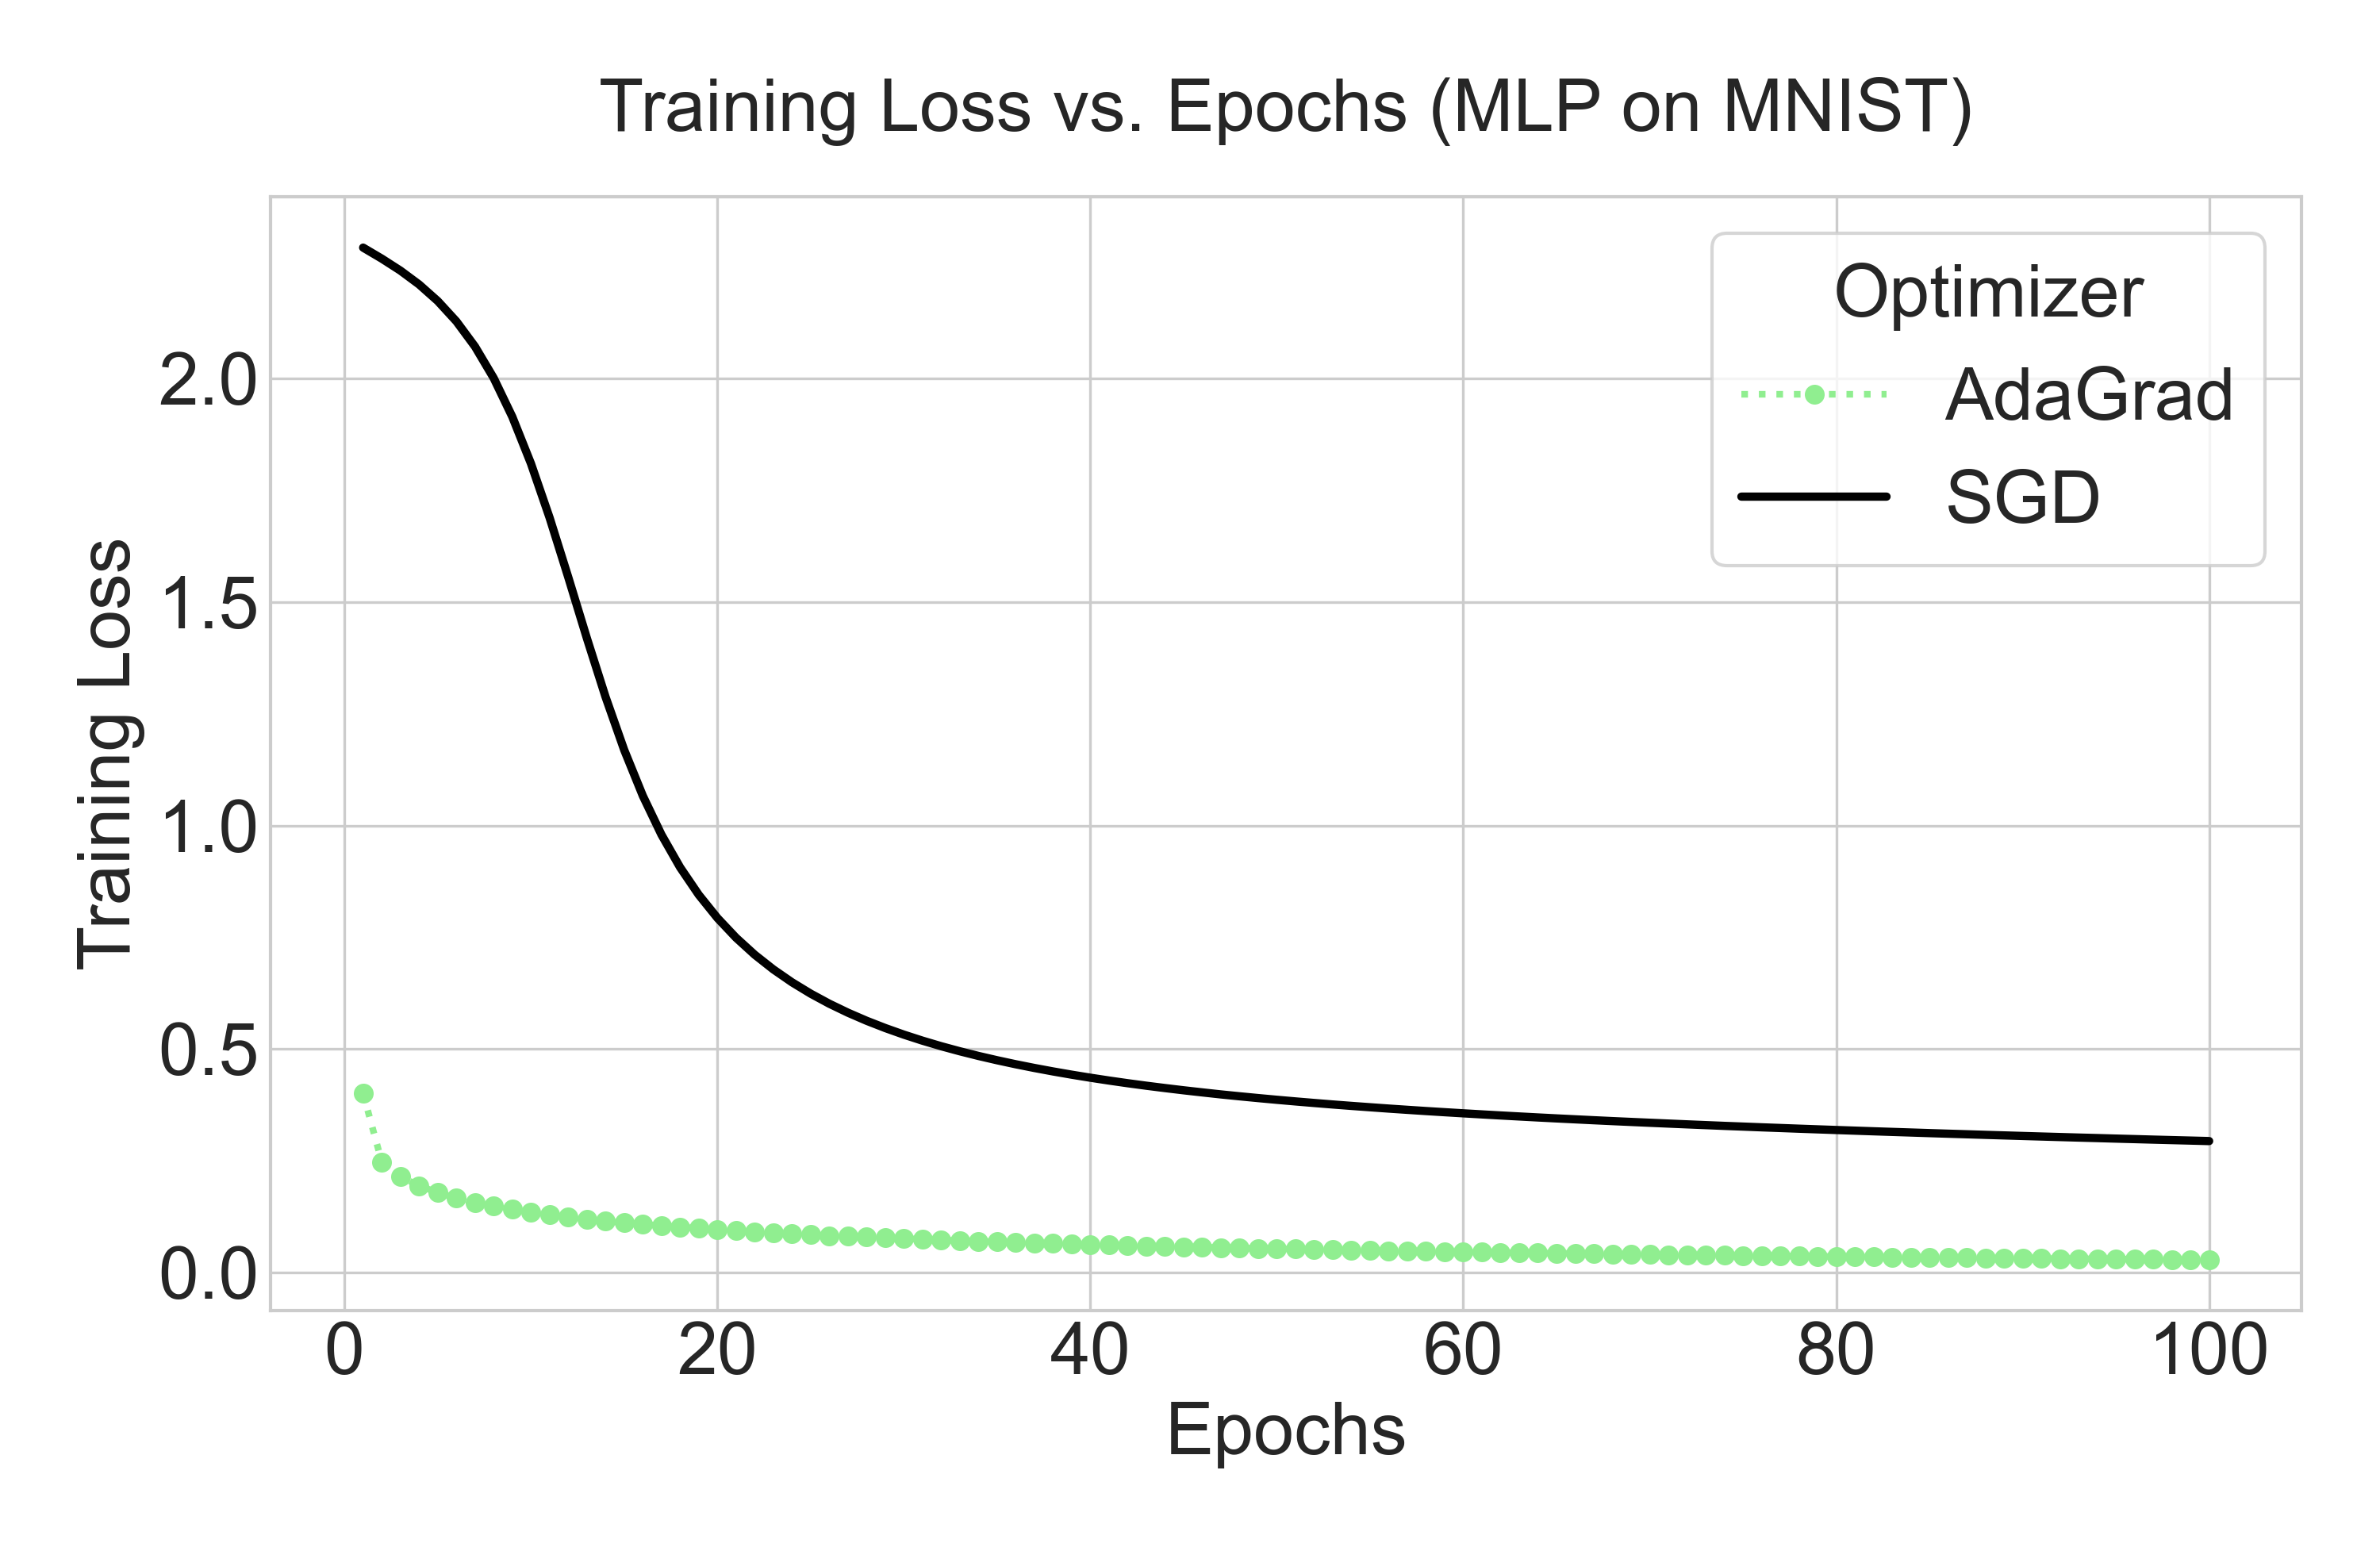
\includegraphics[width=0.48\textwidth]{Analysis_1_Impact_on_Adaptive_Gradient1_mnist_mlp_training_loss.png}} \quad
    \subfloat[MLP Validation Accuracy on MNIST]{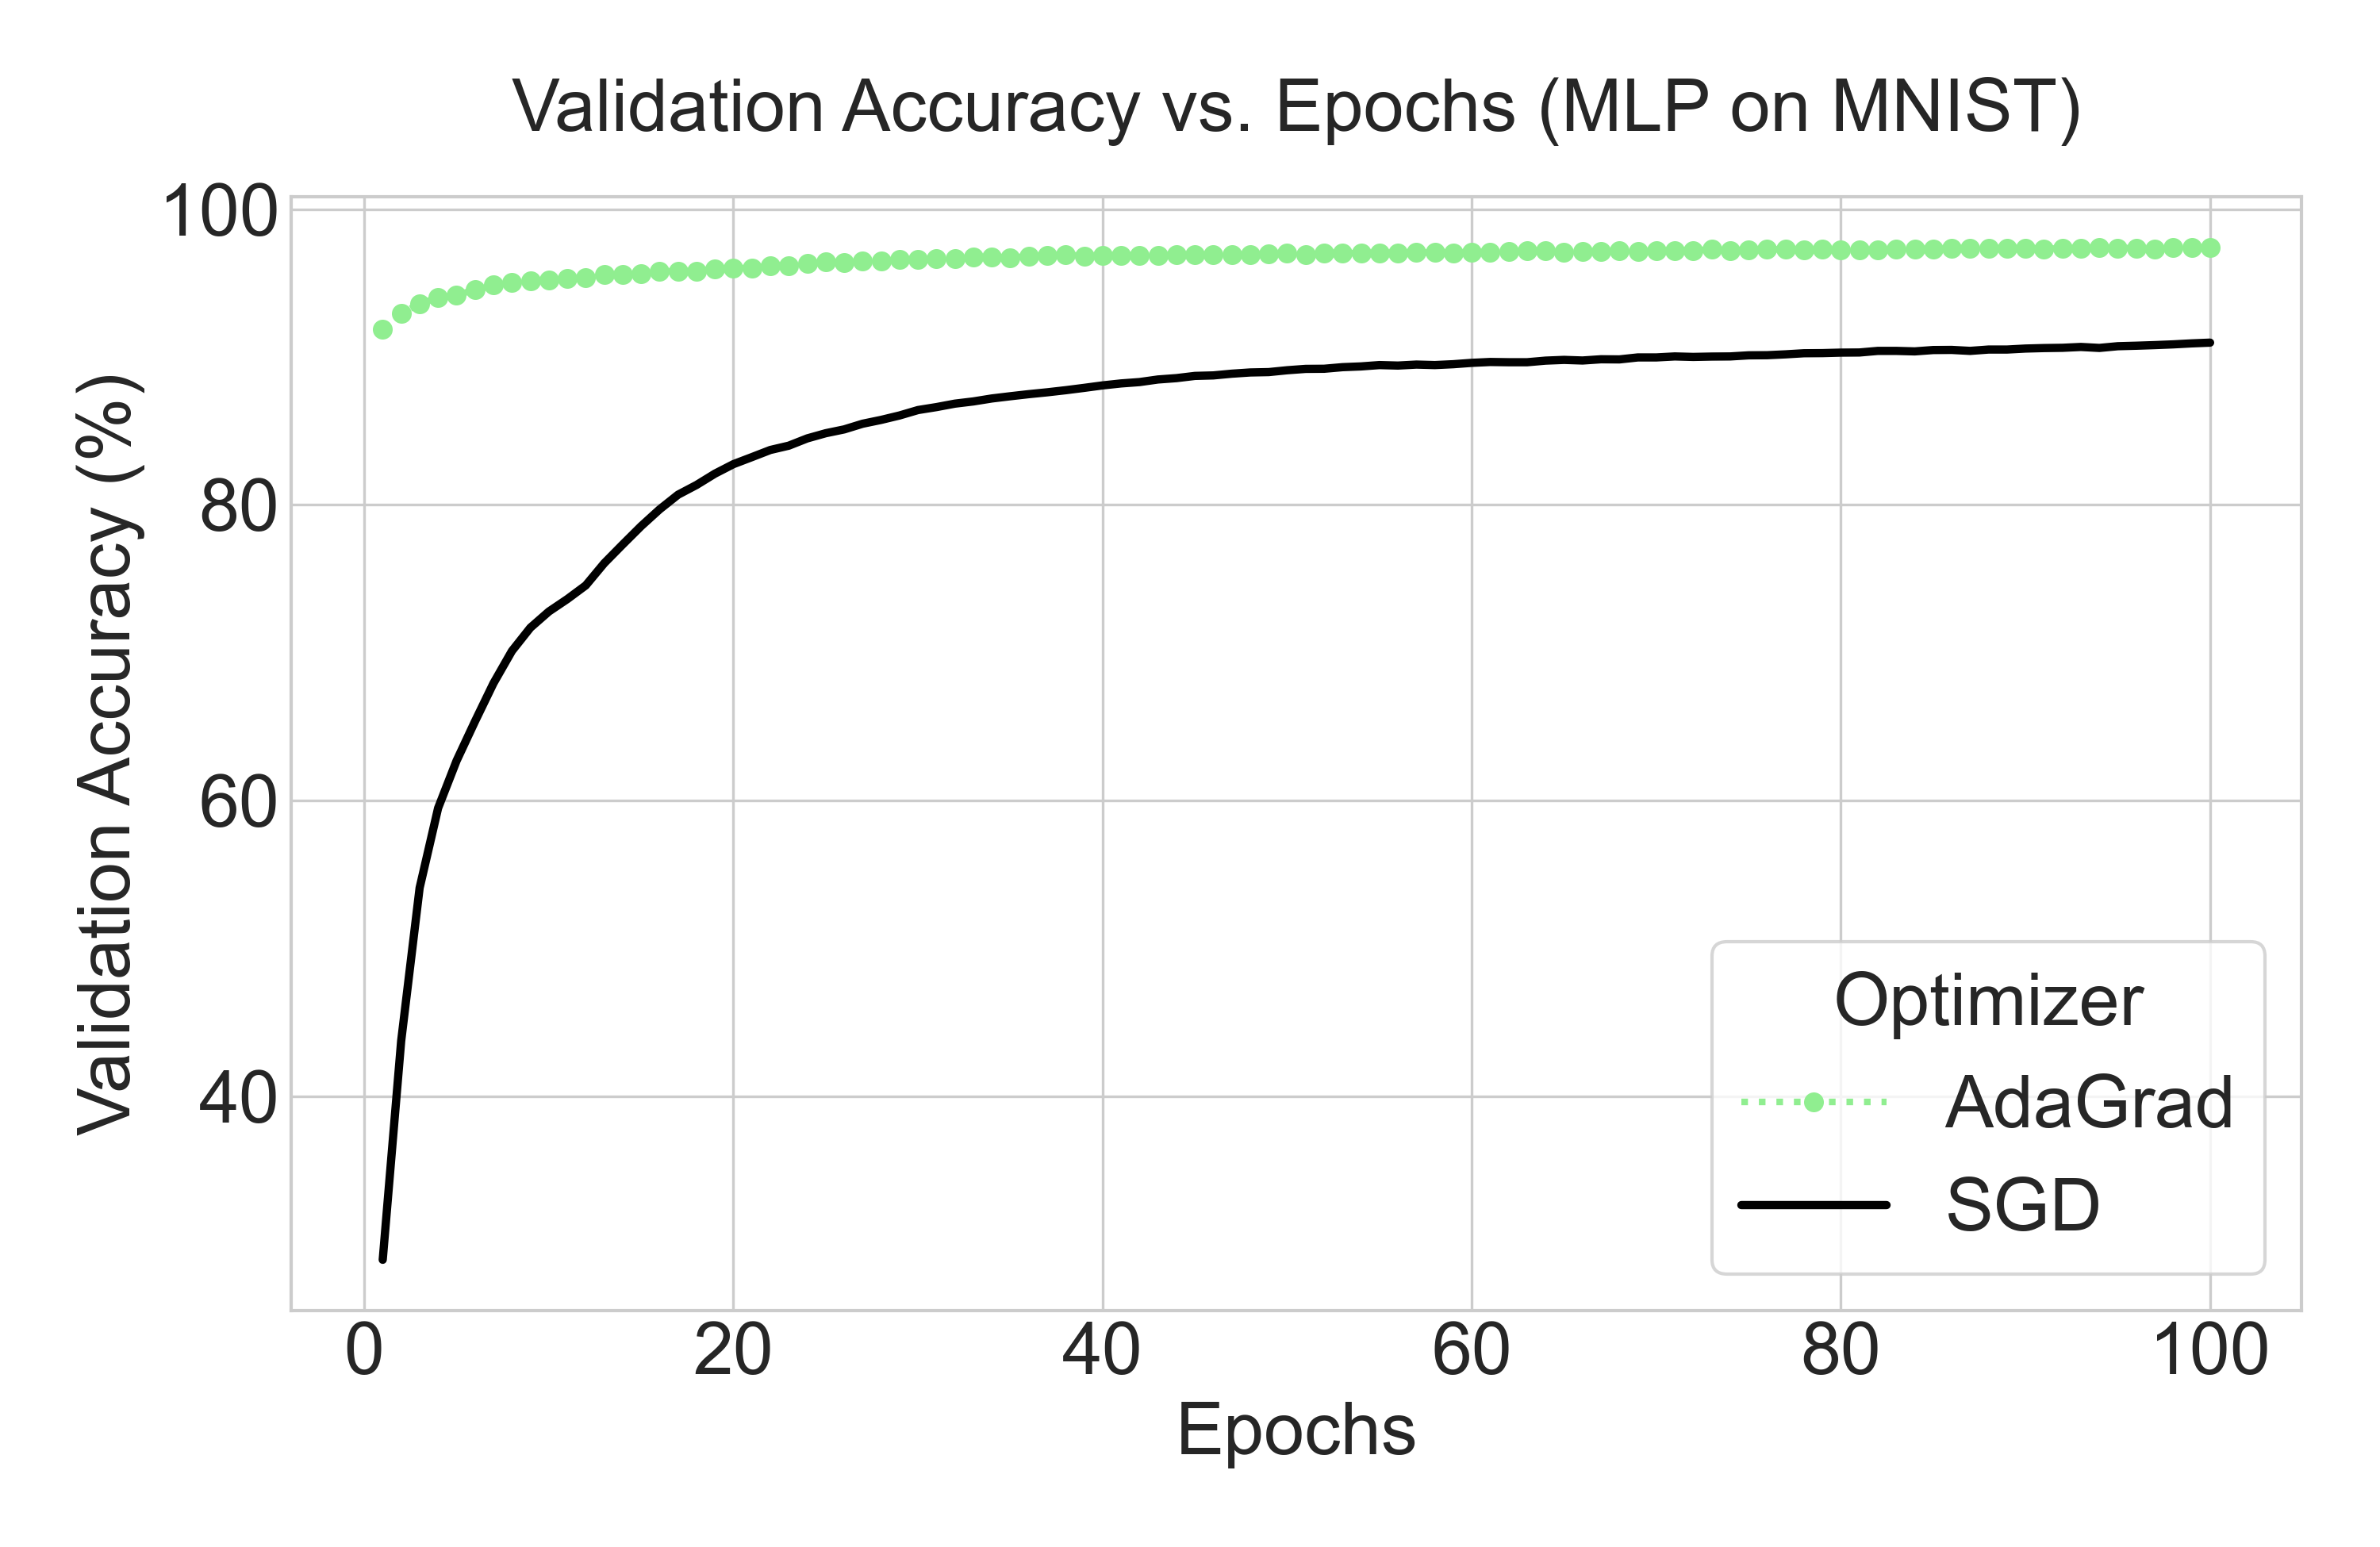
\includegraphics[width=0.48\textwidth]{Analysis_1_Impact_on_Adaptive_Gradient1_mnist_mlp_validation_accuracy.png}} \\
    % CNN row
    \subfloat[CNN Training Loss on CIFAR-10]{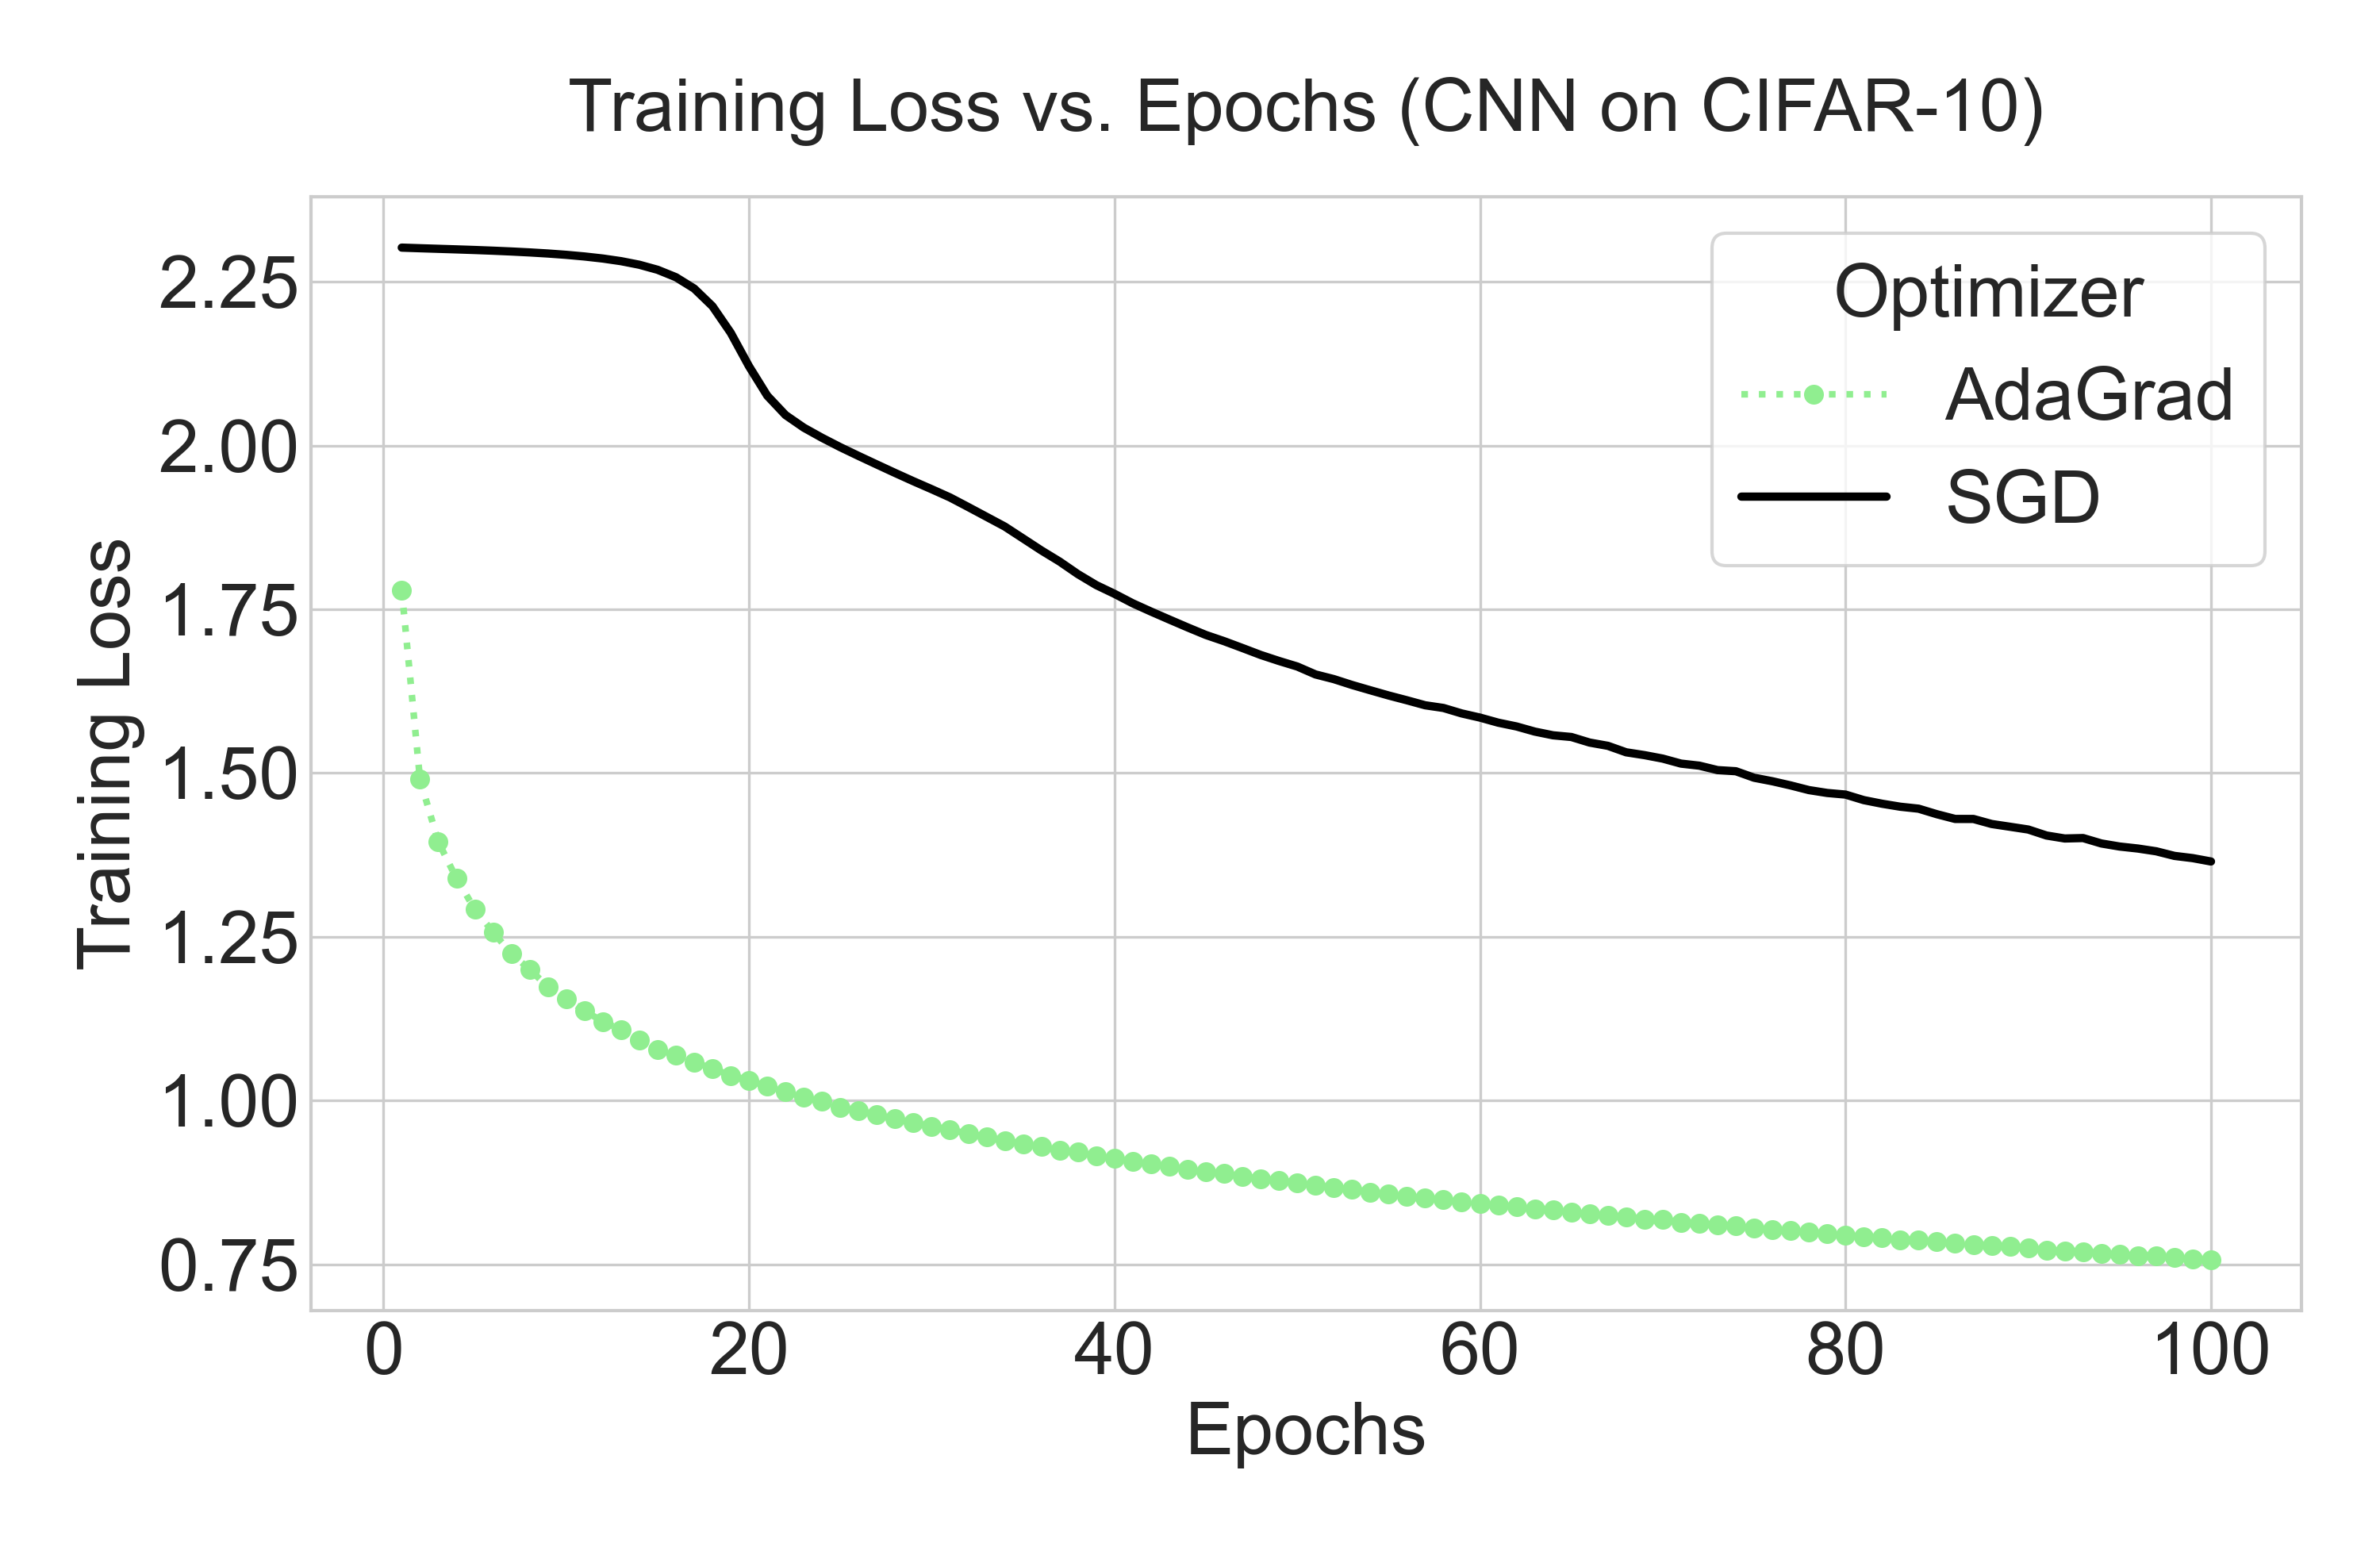
\includegraphics[width=0.48\textwidth]{Analysis_1_Impact_on_Adaptive_Gradient2_cifar10_cnn_training_loss.png}} \quad
    \subfloat[CNN Validation Accuracy on CIFAR-10]{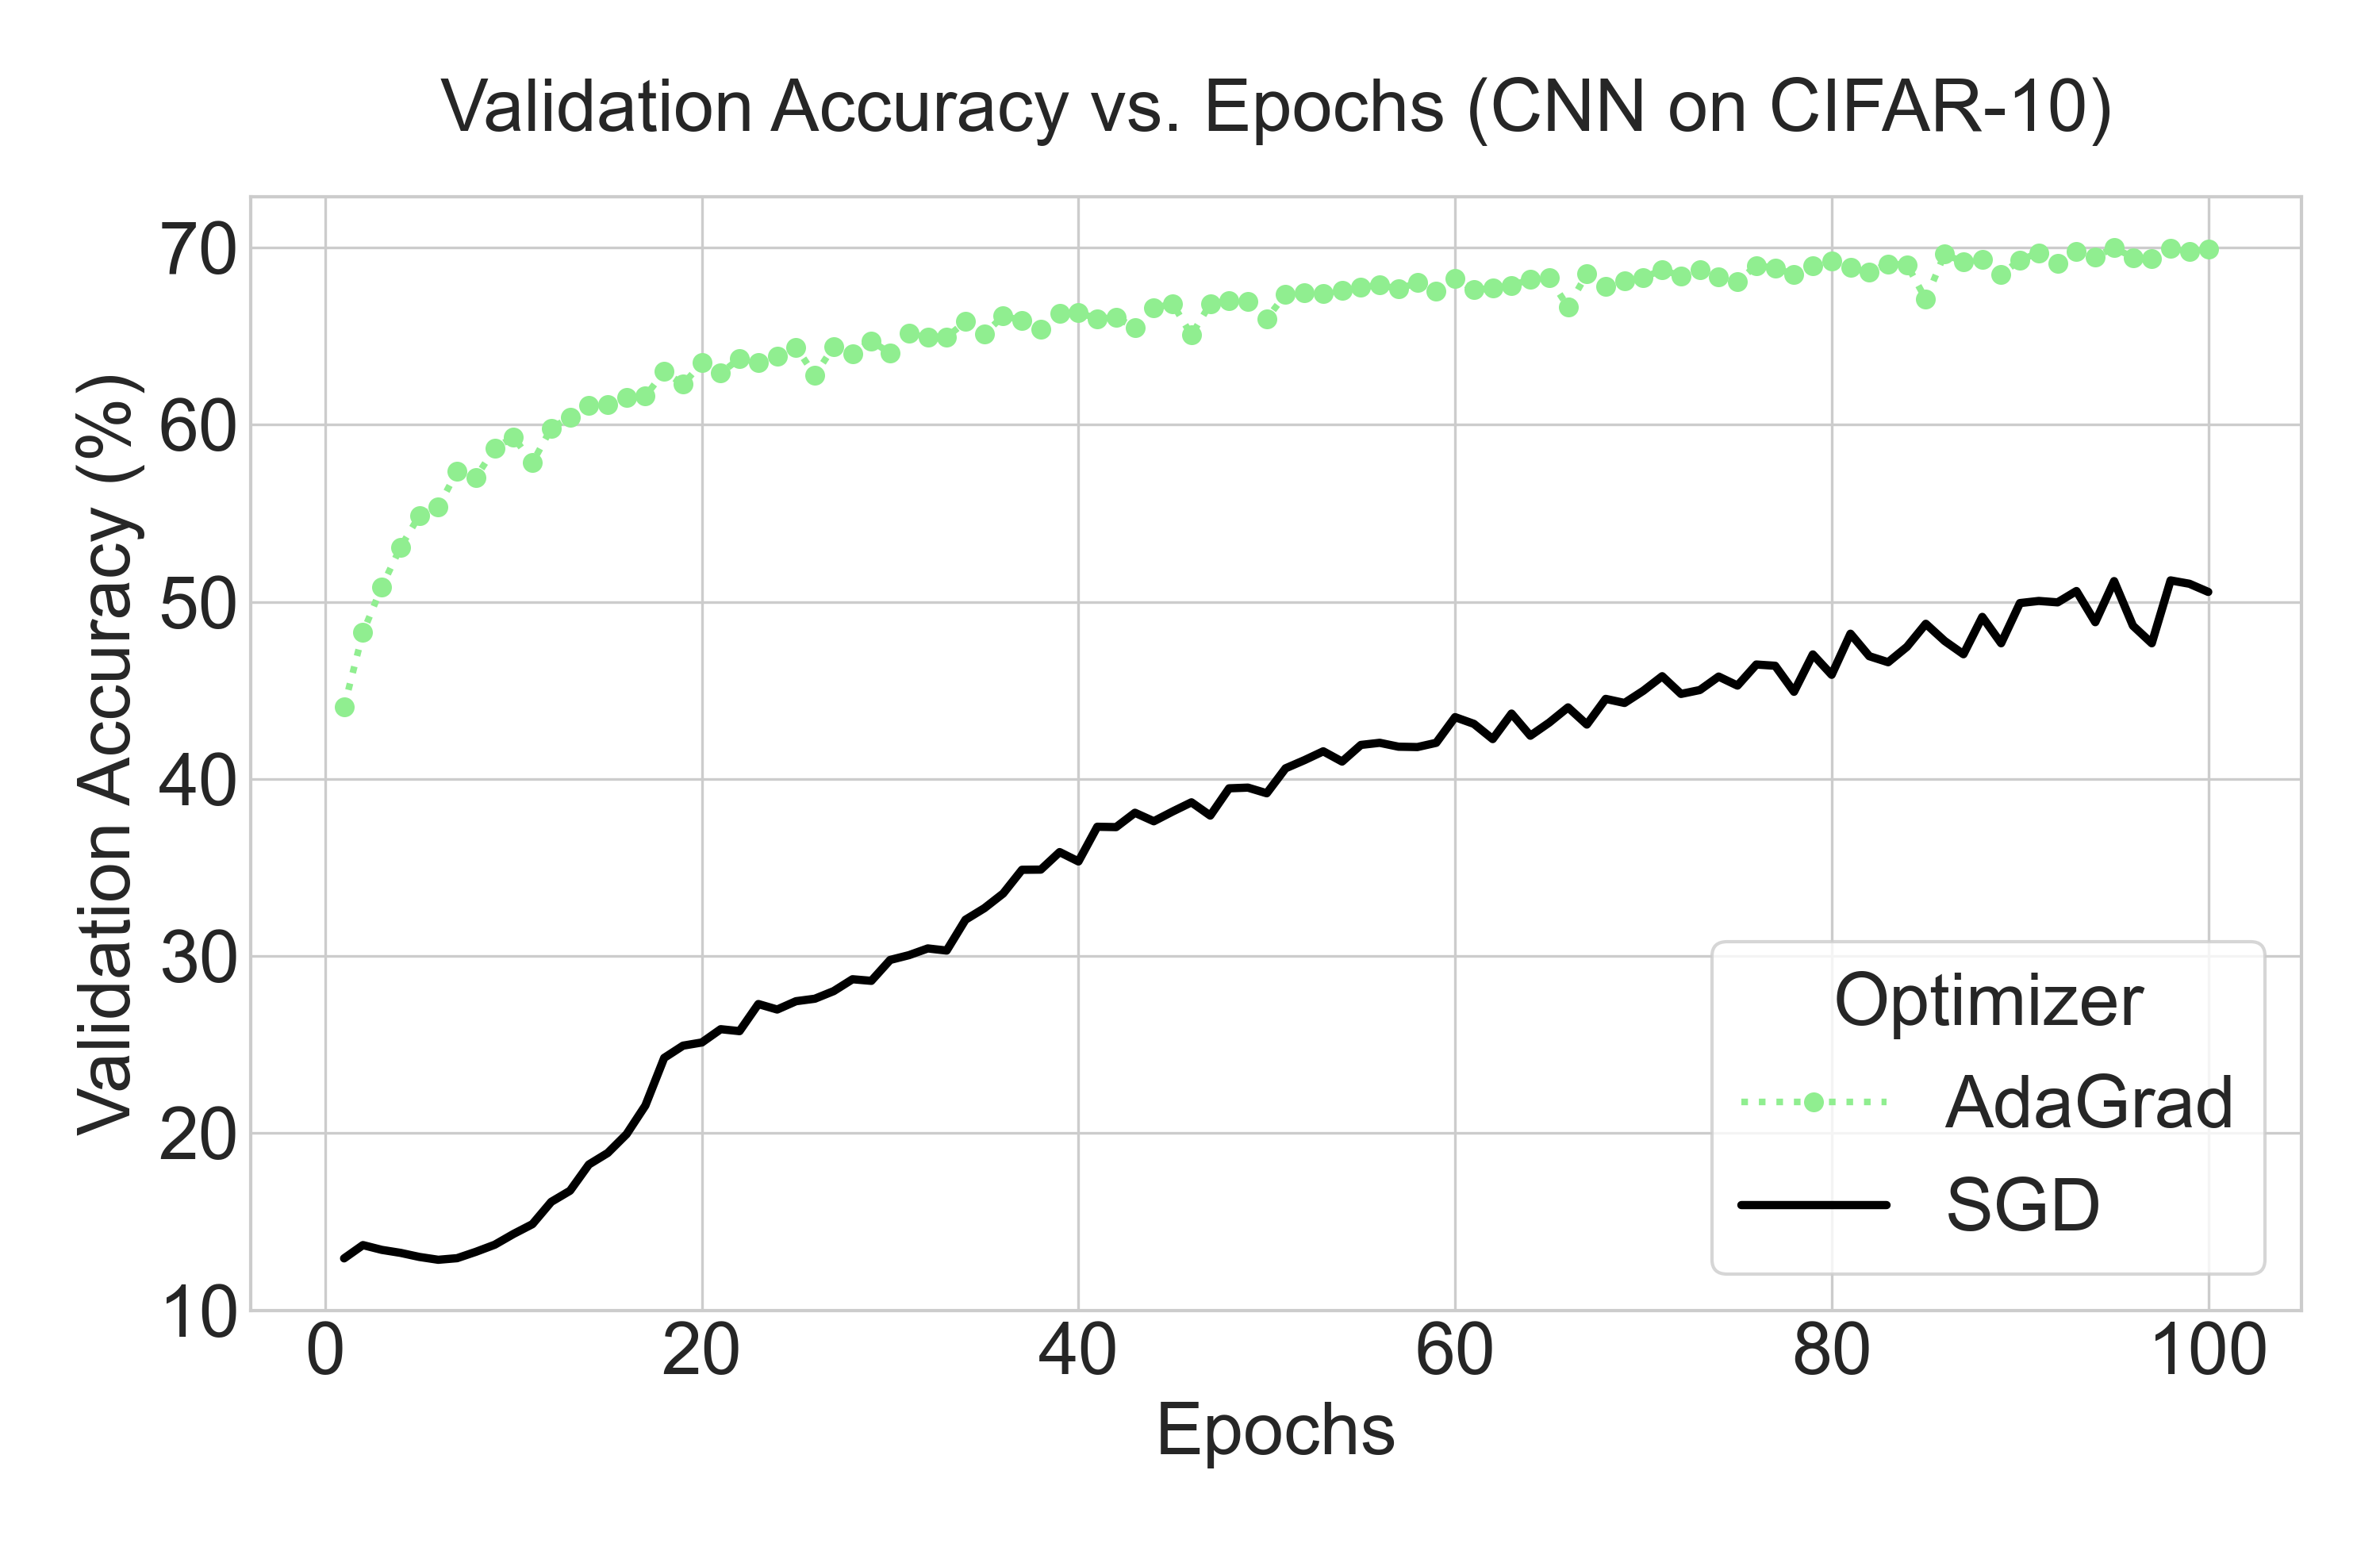
\includegraphics[width=0.48\textwidth]{Analysis_1_Impact_on_Adaptive_Gradient2_cifar10_cnn_validation_accuracy.png}} \\
    % VGG13 row
    \subfloat[VGG13 Training Loss on CIFAR-10]{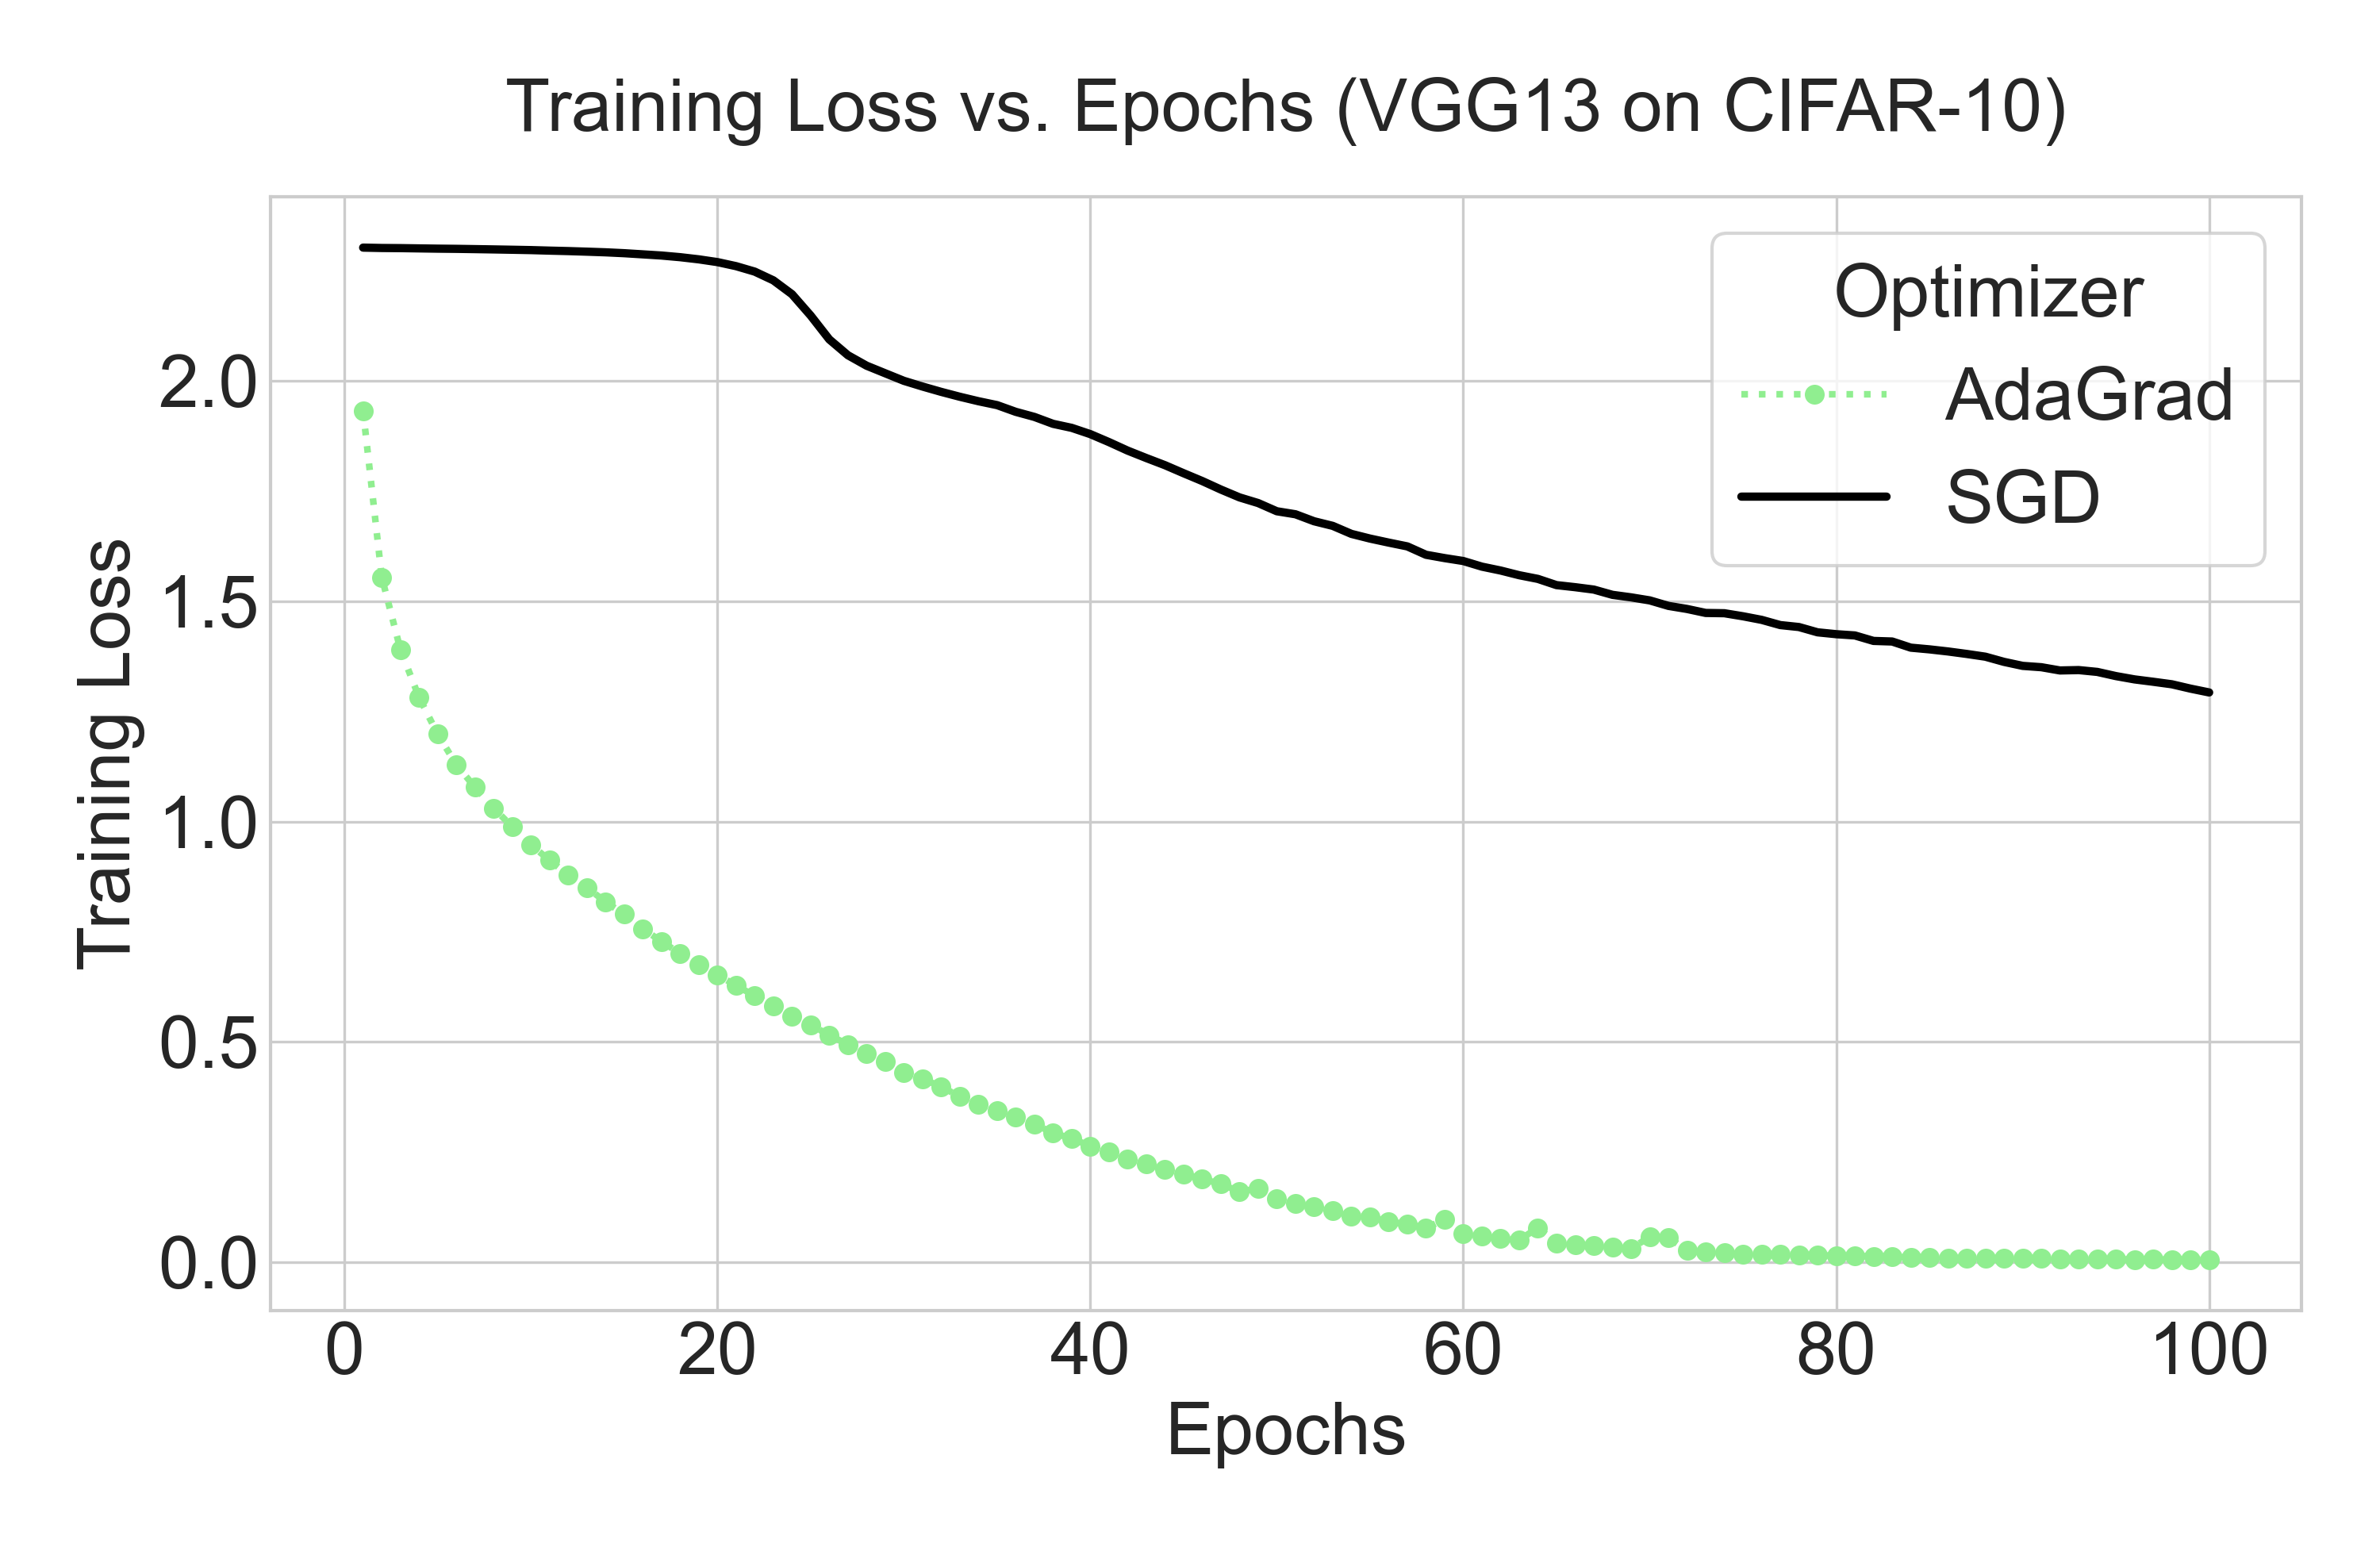
\includegraphics[width=0.48\textwidth]{Analysis_1_Impact_on_Adaptive_Gradient3_cifar_vgg13_training_loss.png}} \quad
    \subfloat[VGG13 Validation Accuracy on CIFAR-10]{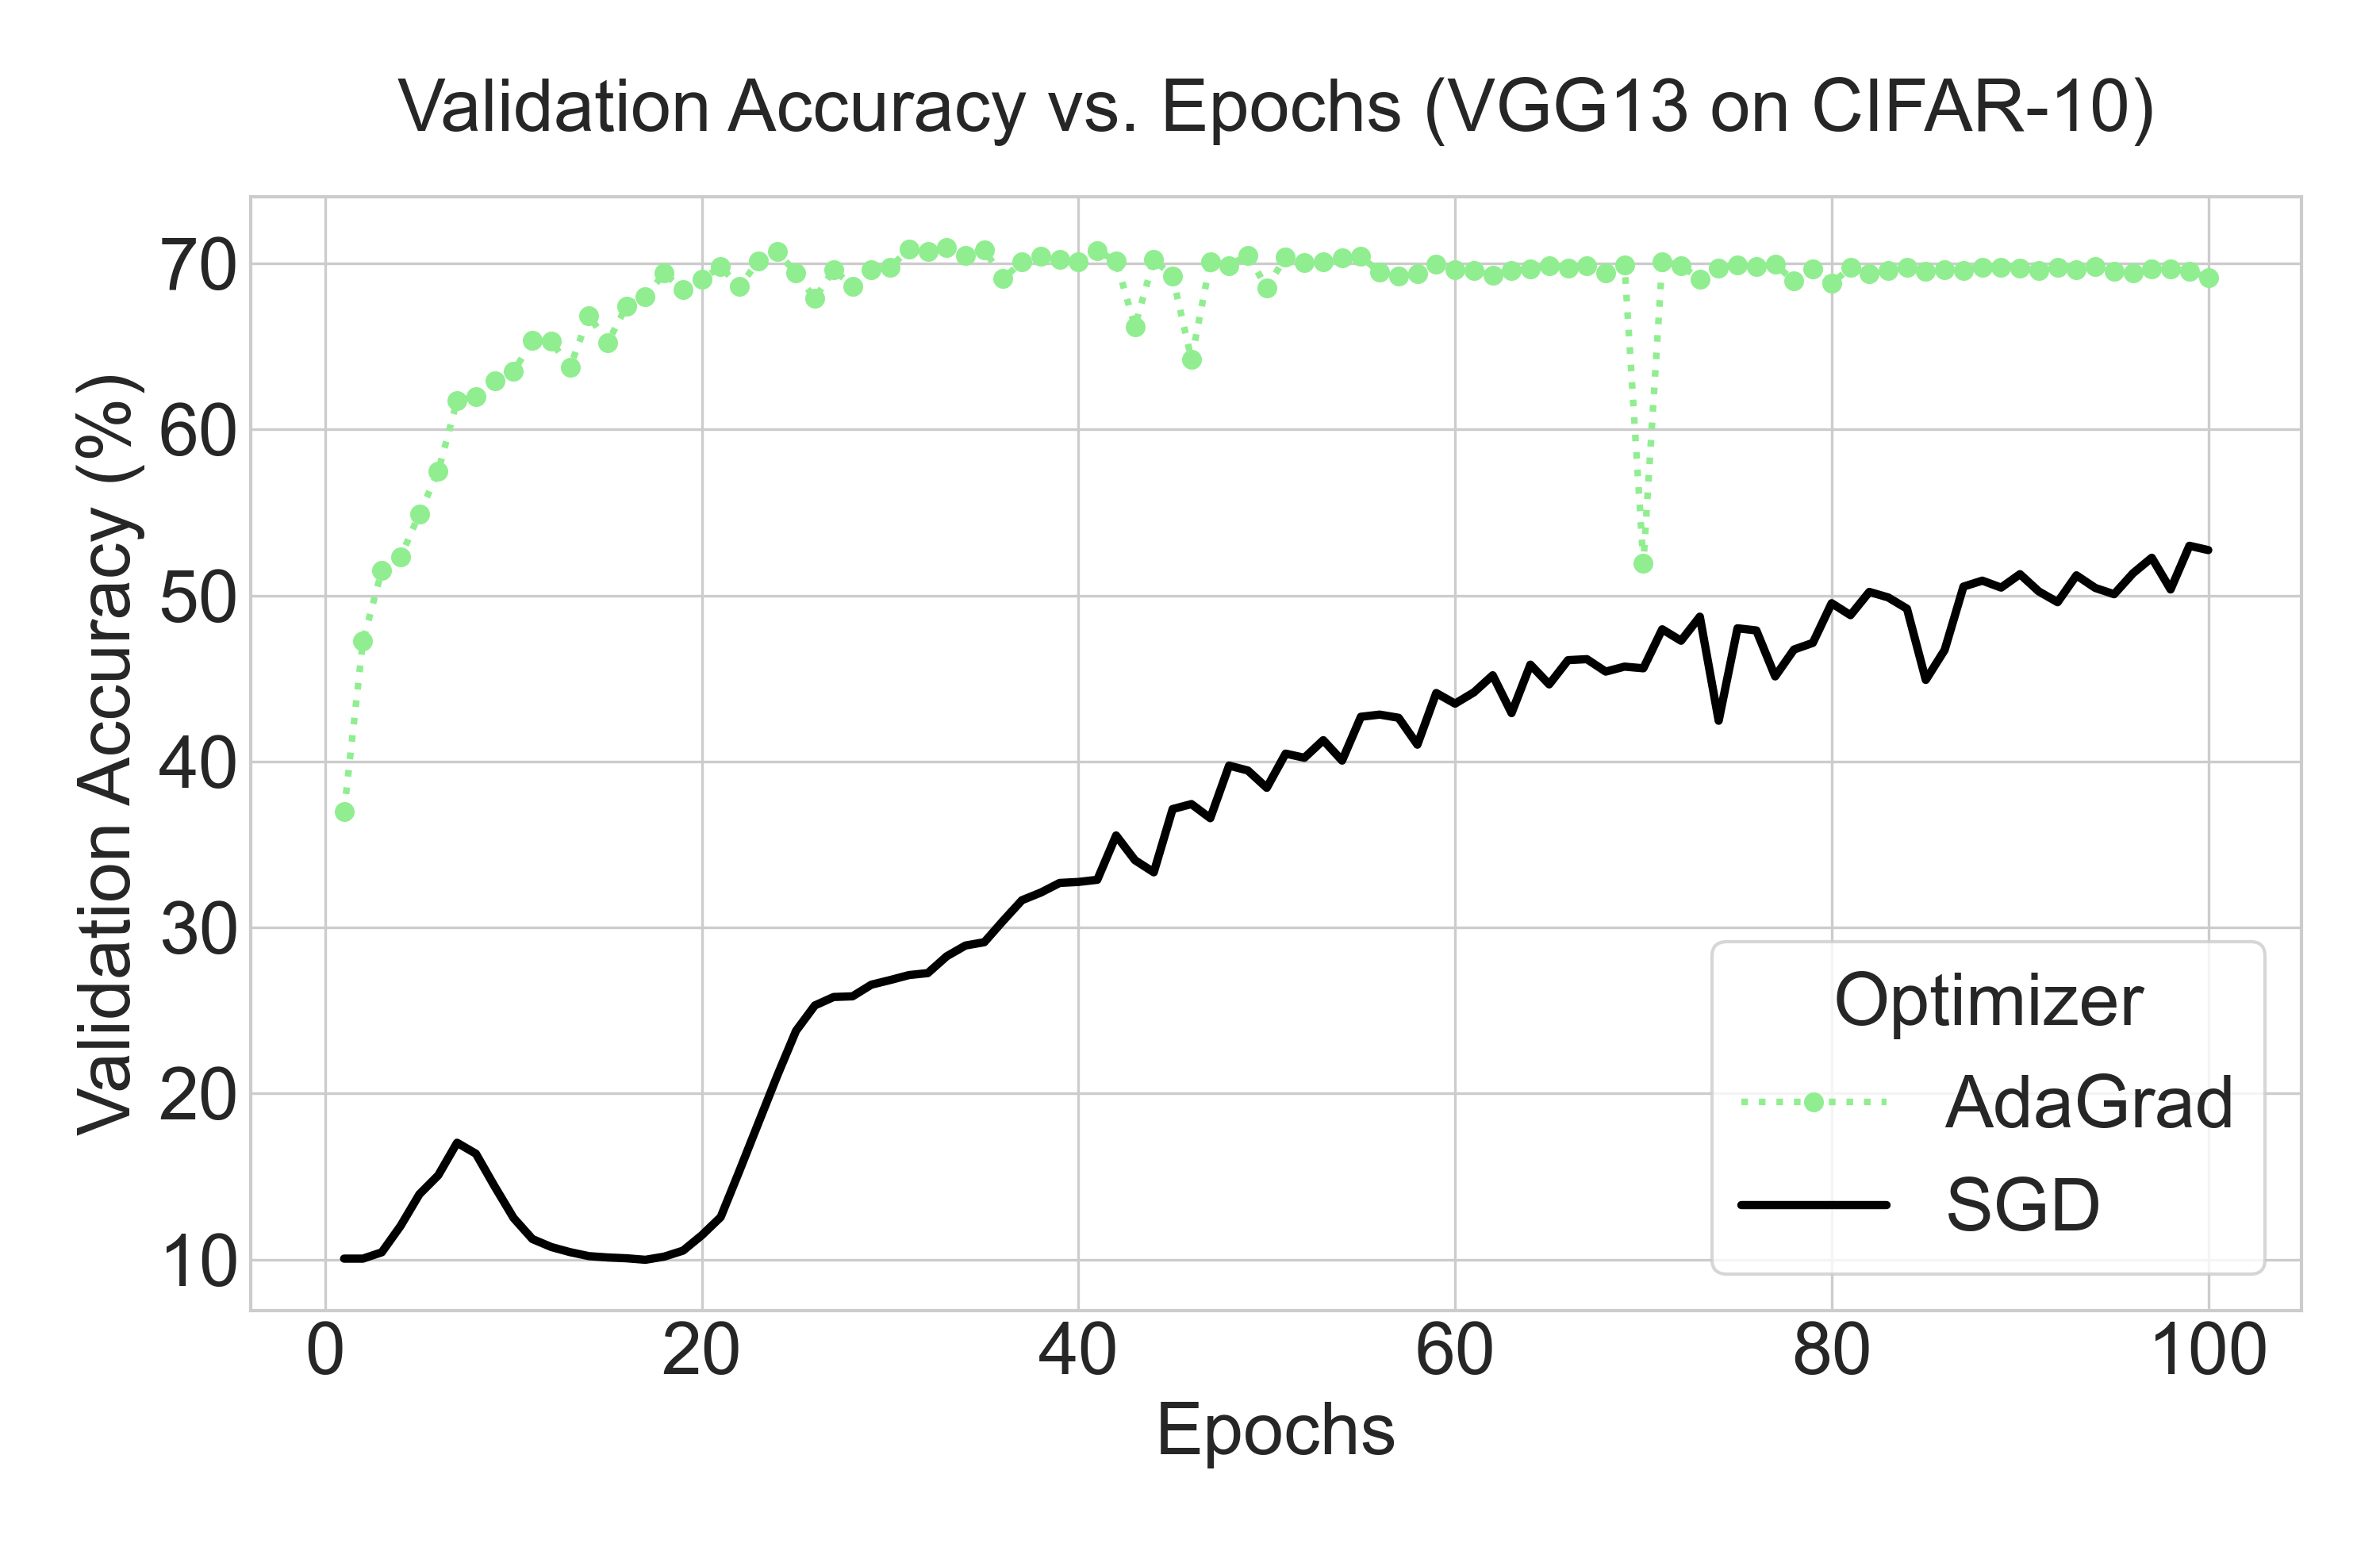
\includegraphics[width=0.48\textwidth]{Analysis_1_Impact_on_Adaptive_Gradient3_cifar_vgg13_validation_accuracy.png}}
    \caption{Impact of adaptive gradient: baseline method (SGD, black line) vs. baseline method with adpative gradient (AdaGrad, green line)}
    \label{fig:performance_comparison}
\end{figure}

The above figures show the training performance of the three models on the MNIST and CIFAR-10 datasets. 

The table below presents their final accuracy on the test set:


\begin{table}[H]
\centering
\caption{Final Test Accuracy (AdaGrad vs. SGD)}
\label{tab:final_accuracy_transposed}
\begin{tabular}{|l|c|c|c|}
\hline
        & MLP on MNIST & CNN on CIFAR-10 & VGG13 on CIFAR-10 \\ \hline
SGD     & 91.82\%      & 50.64\%         & 52.68\%           \\ \hline
AdaGrad & \textbf{97.77\%} & \textbf{69.98\%}  & \textbf{68.11\%}    \\ \hline
\end{tabular}
\end{table}

From the results of Experiment.1, we can see that AdaGrad performs significantly better than SGD.

From the training loss graphs, we can see that \textbf{AdaGrad shows a faster convergence speed in all three training runs.} At the beginning of training, the curves drop more steeply for AdaGrad, while SGD decreases more slowly. After 100 epochs, the final loss values of AdaGrad are significantly lower than those of SGD.

Compared to SGD, AdaGrad uses an adaptive learning rate. This allows AdaGrad to find a more suitable update step size during the early stages of training, leading to faster learning and convergence.

From the validation accuracy graphs, we can observe that AdaGrad reaches a higher accuracy level more quickly. Its curve is also smoother and shows less fluctuation than SGD. This demonstrates the advantage of AdaGrad’s adaptive learning rate, which not only speeds up training but also helps the model transition more smoothly in complex gradient regions. \textbf{Thus, AdaGrad has better training speed and training stability.}

Finally, from the test accuracy results, AdaGrad achieves higher accuracy across all three tasks. \textbf{The result confirms that AdaGrad has better generalization ability compared to SGD.}




%--------------------------------------------
\subsection{Exponential Moving Average}


\begin{figure}[htbp]
    \centering
    % MLP row
    \subfloat[MLP Loss on MNIST]{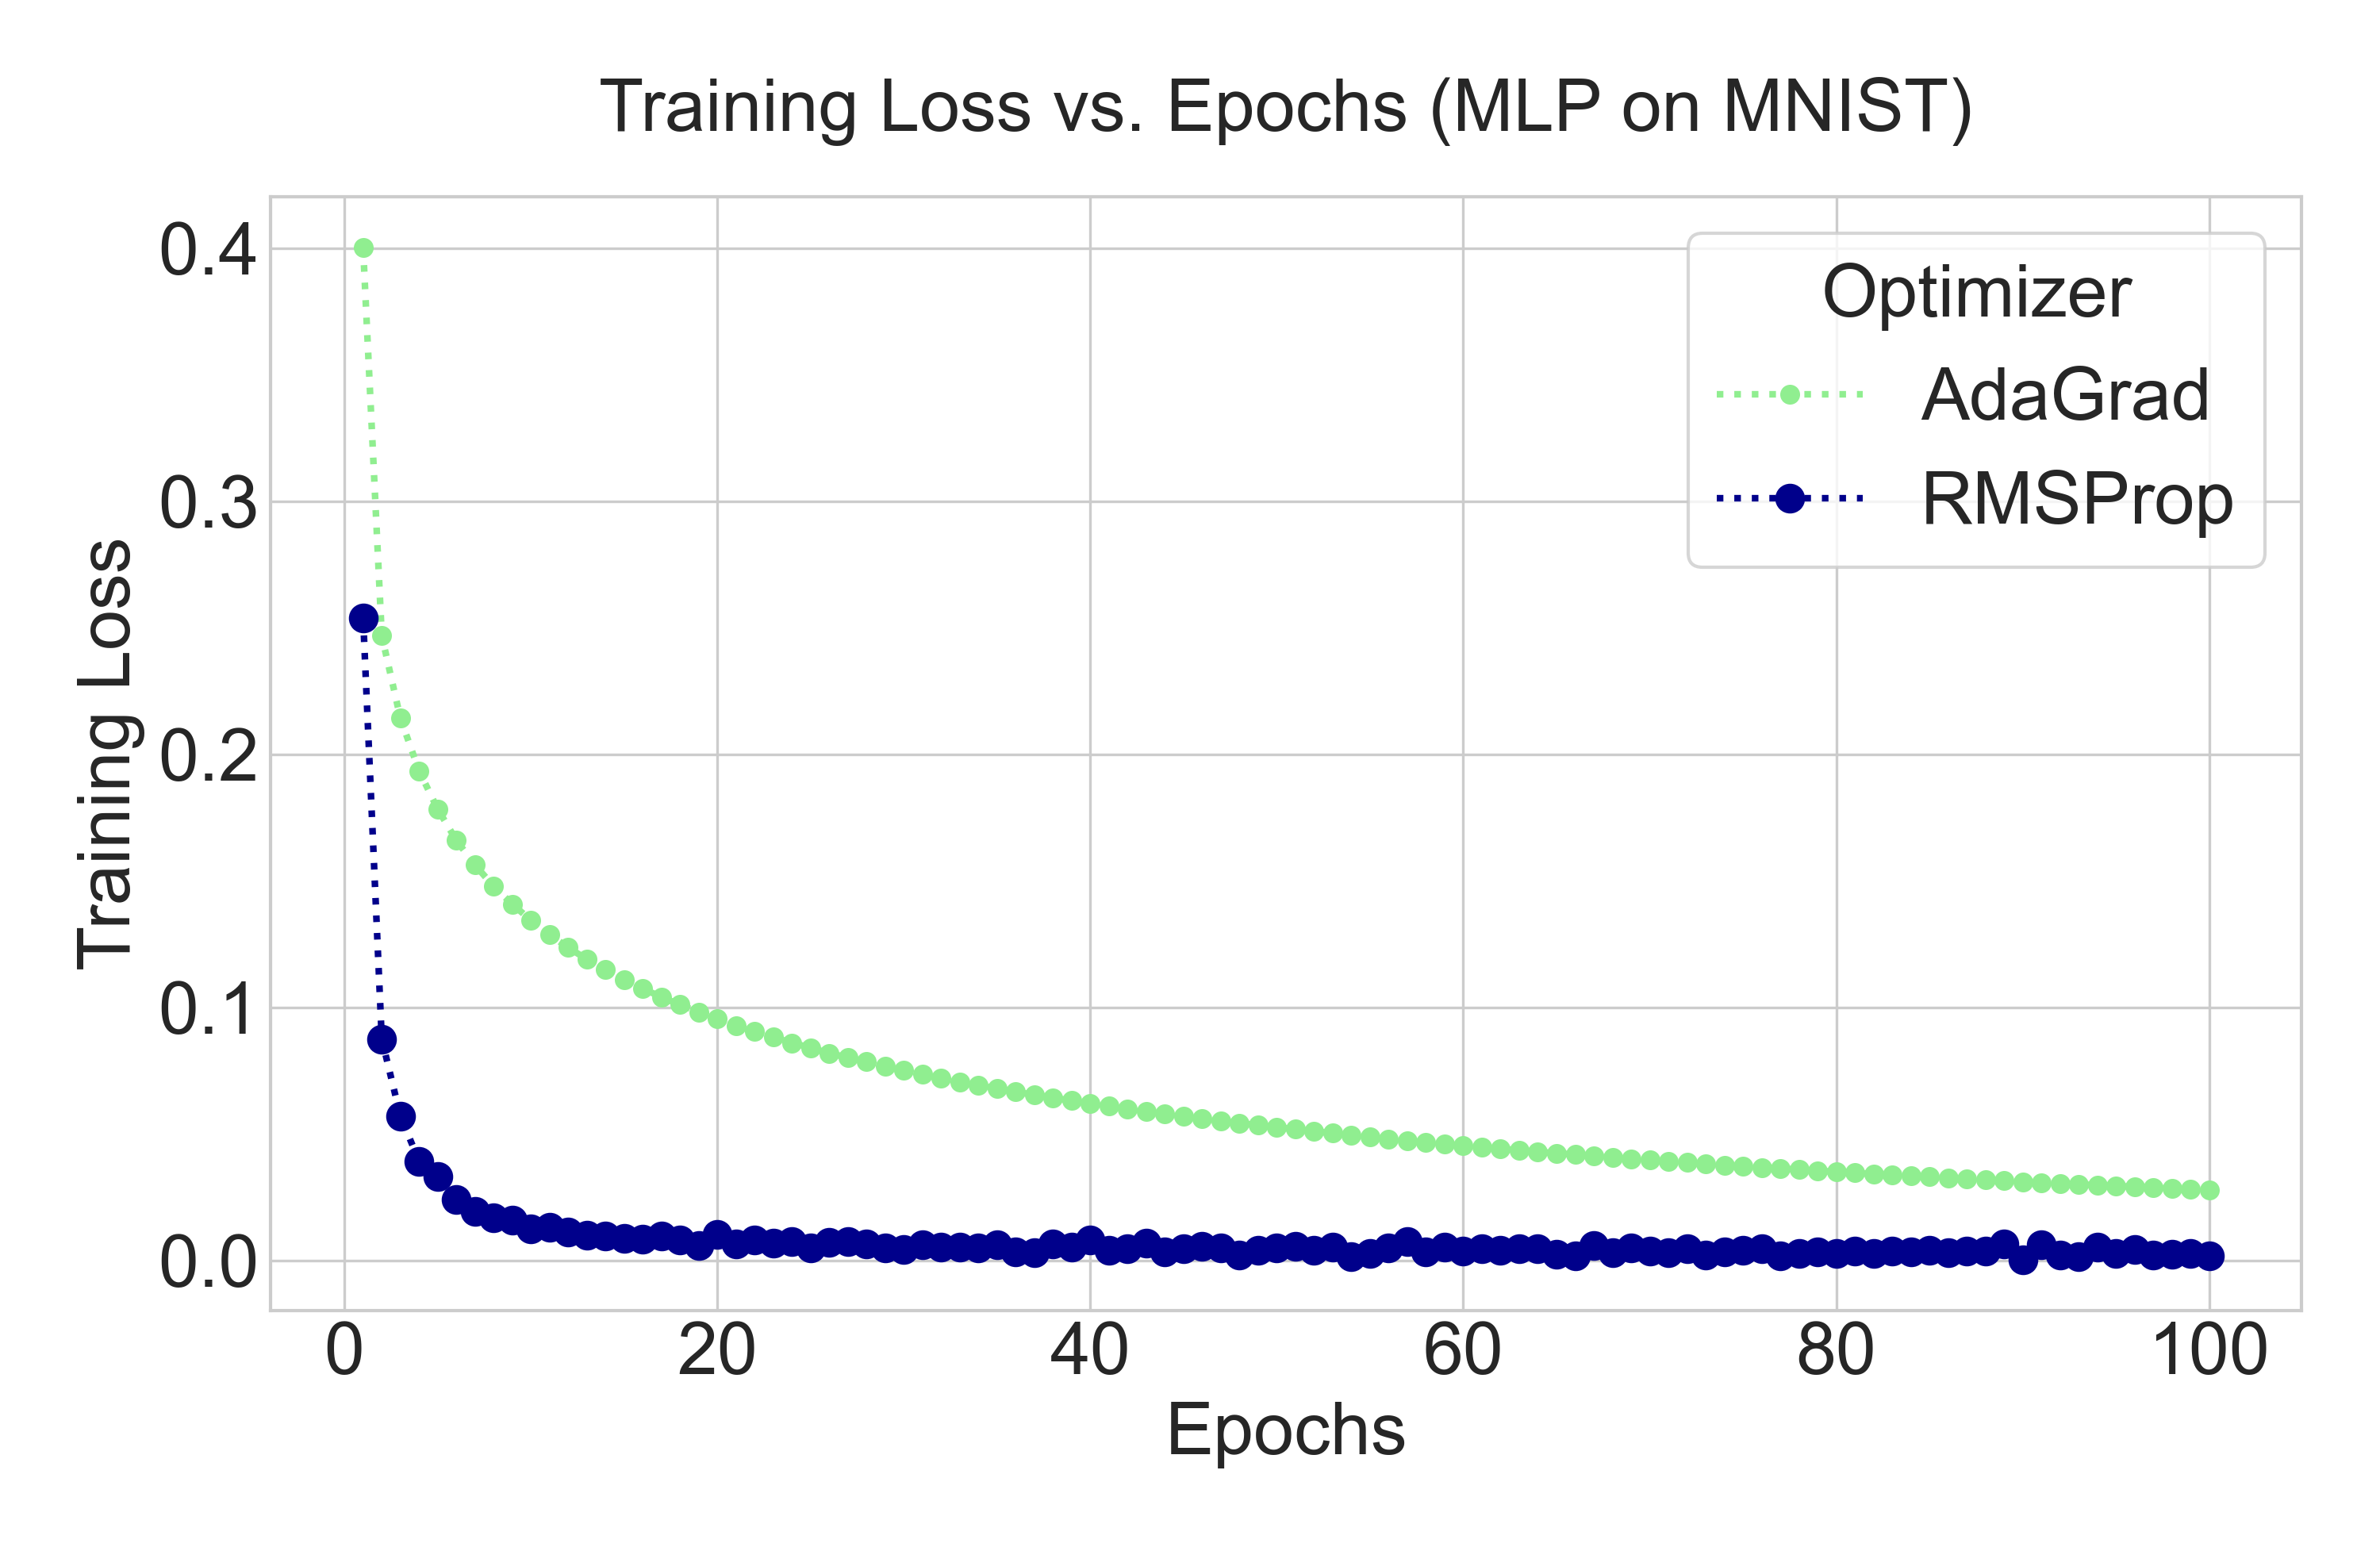
\includegraphics[width=0.48\textwidth]{Analysis_2_Impact_of_EMA1_mnist_mlp_training_loss.png}} \quad
    \subfloat[MLP Accuracy on MNIST]{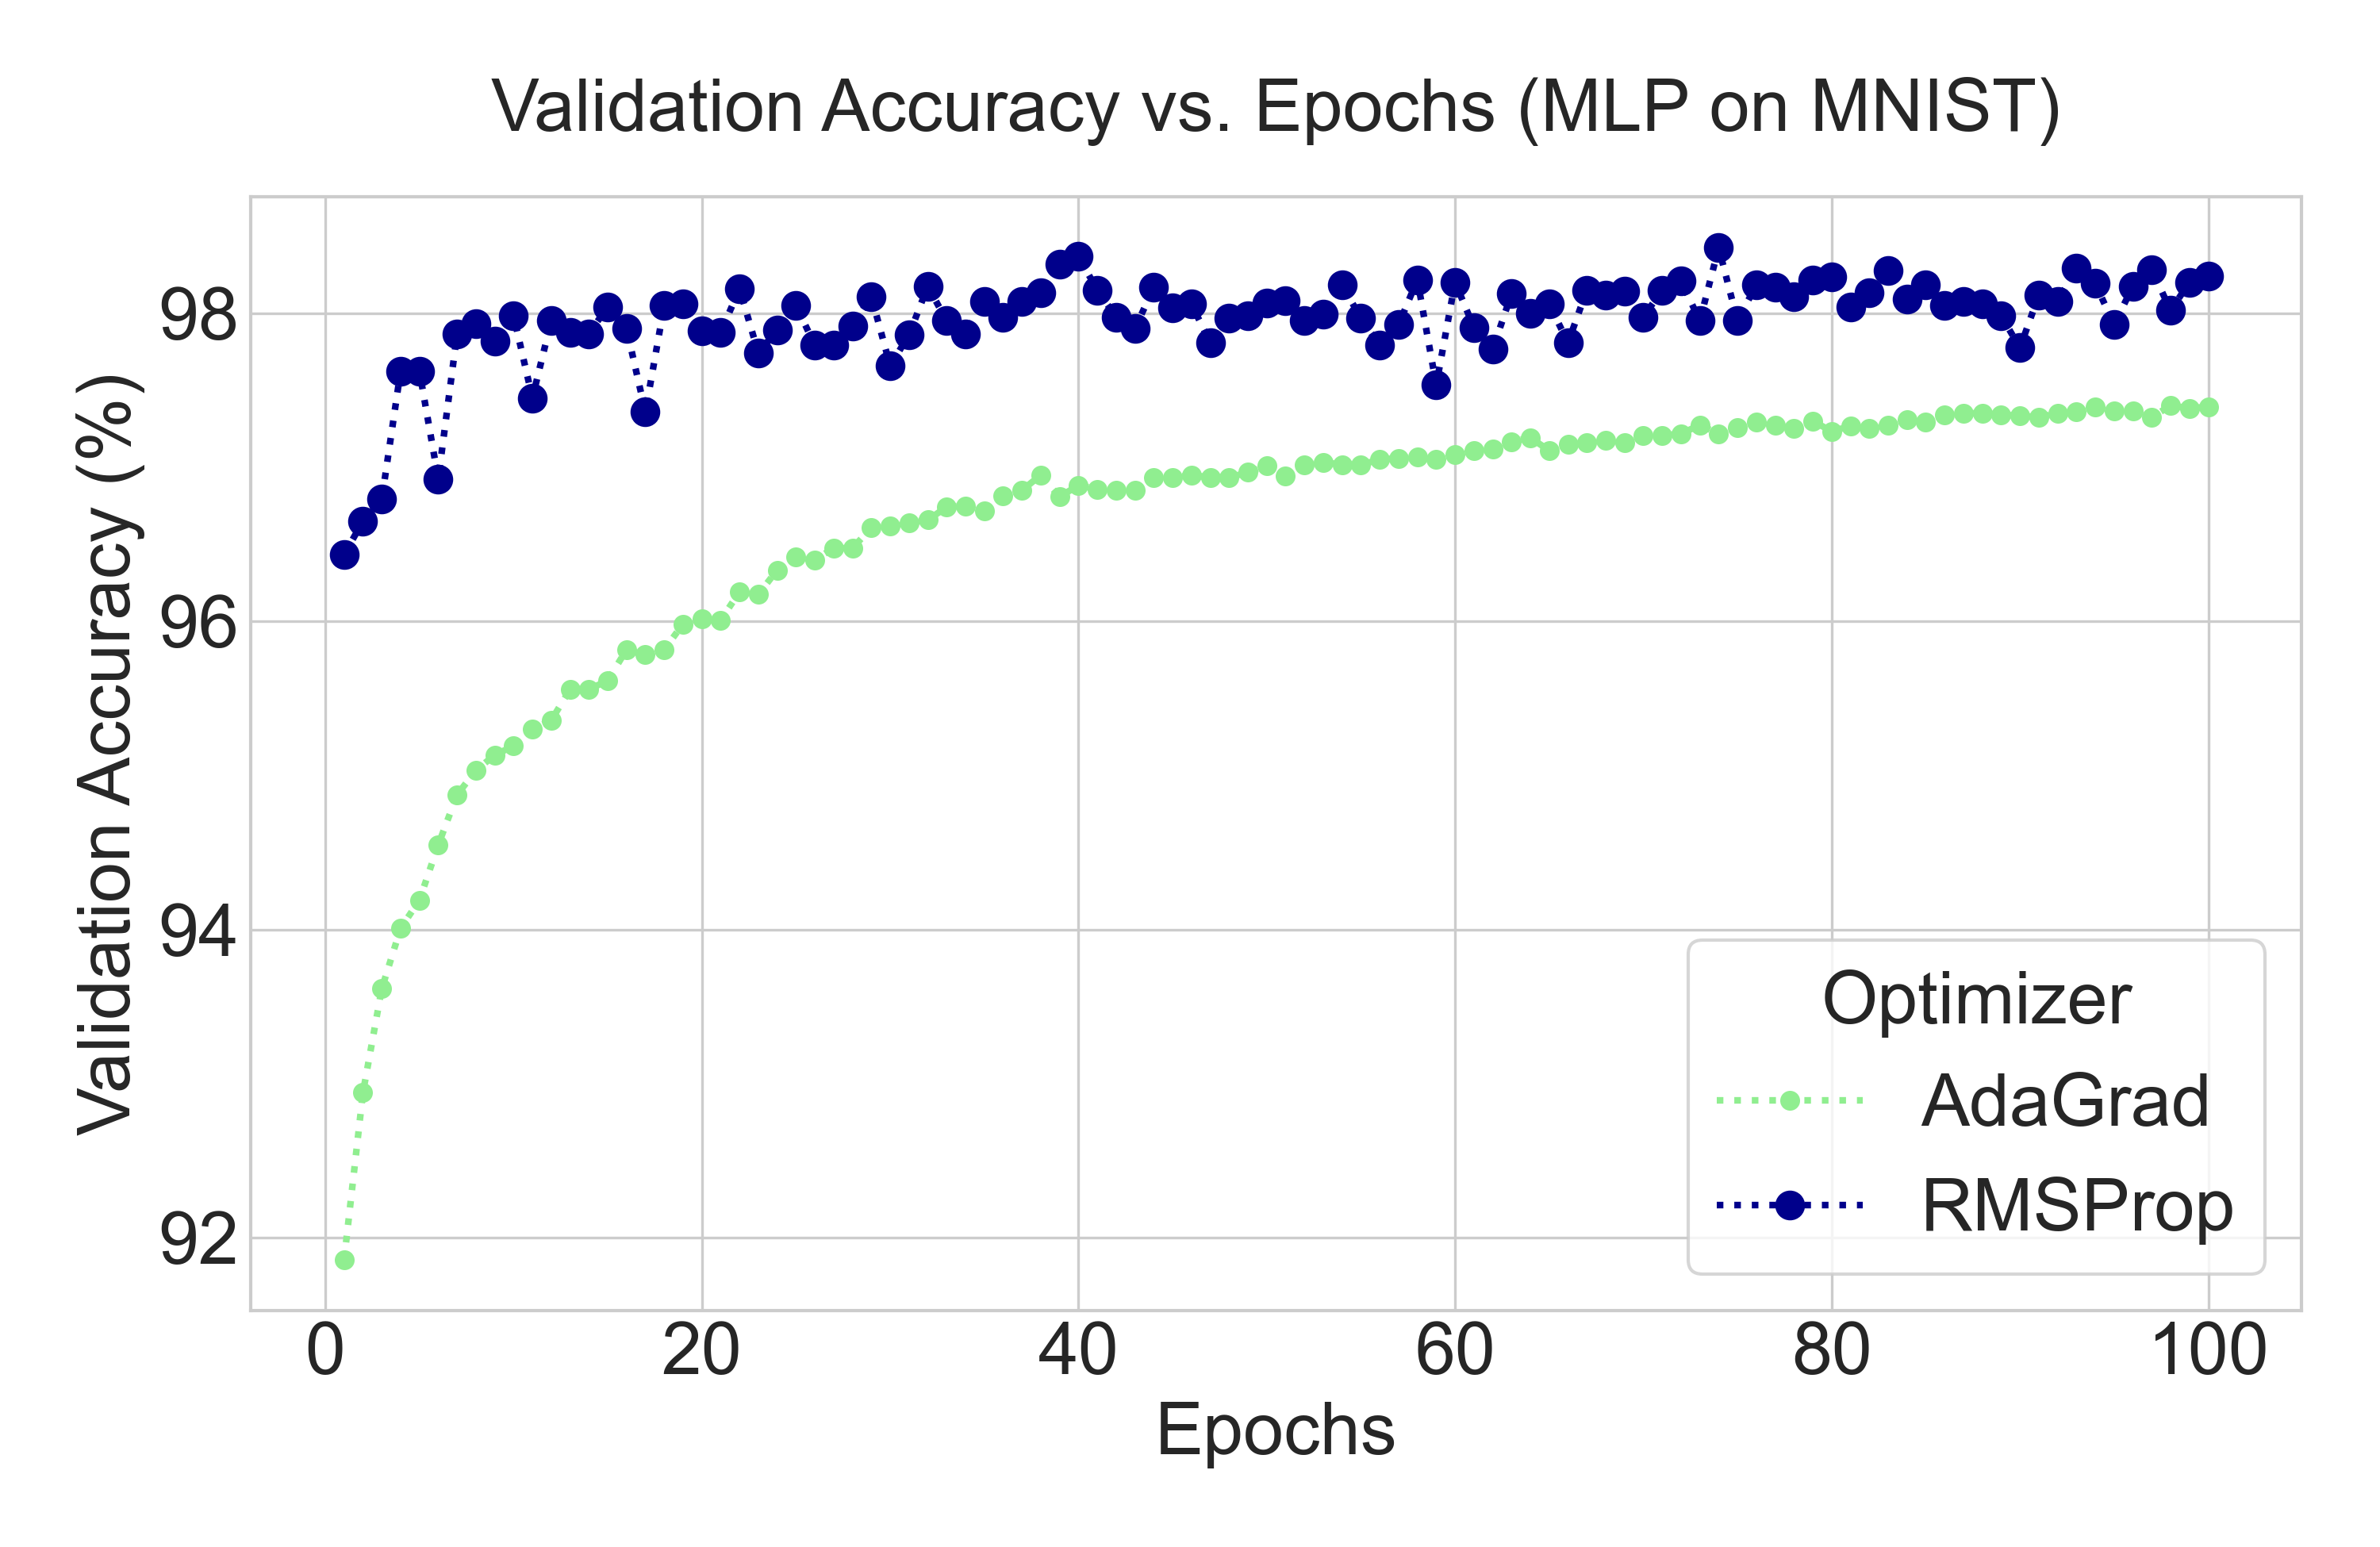
\includegraphics[width=0.48\textwidth]{Analysis_2_Impact_of_EMA1_mnist_mlp_validation_accuracy.png}} \\
    % CNN row
    \subfloat[CNN Loss on CIFAR-10]{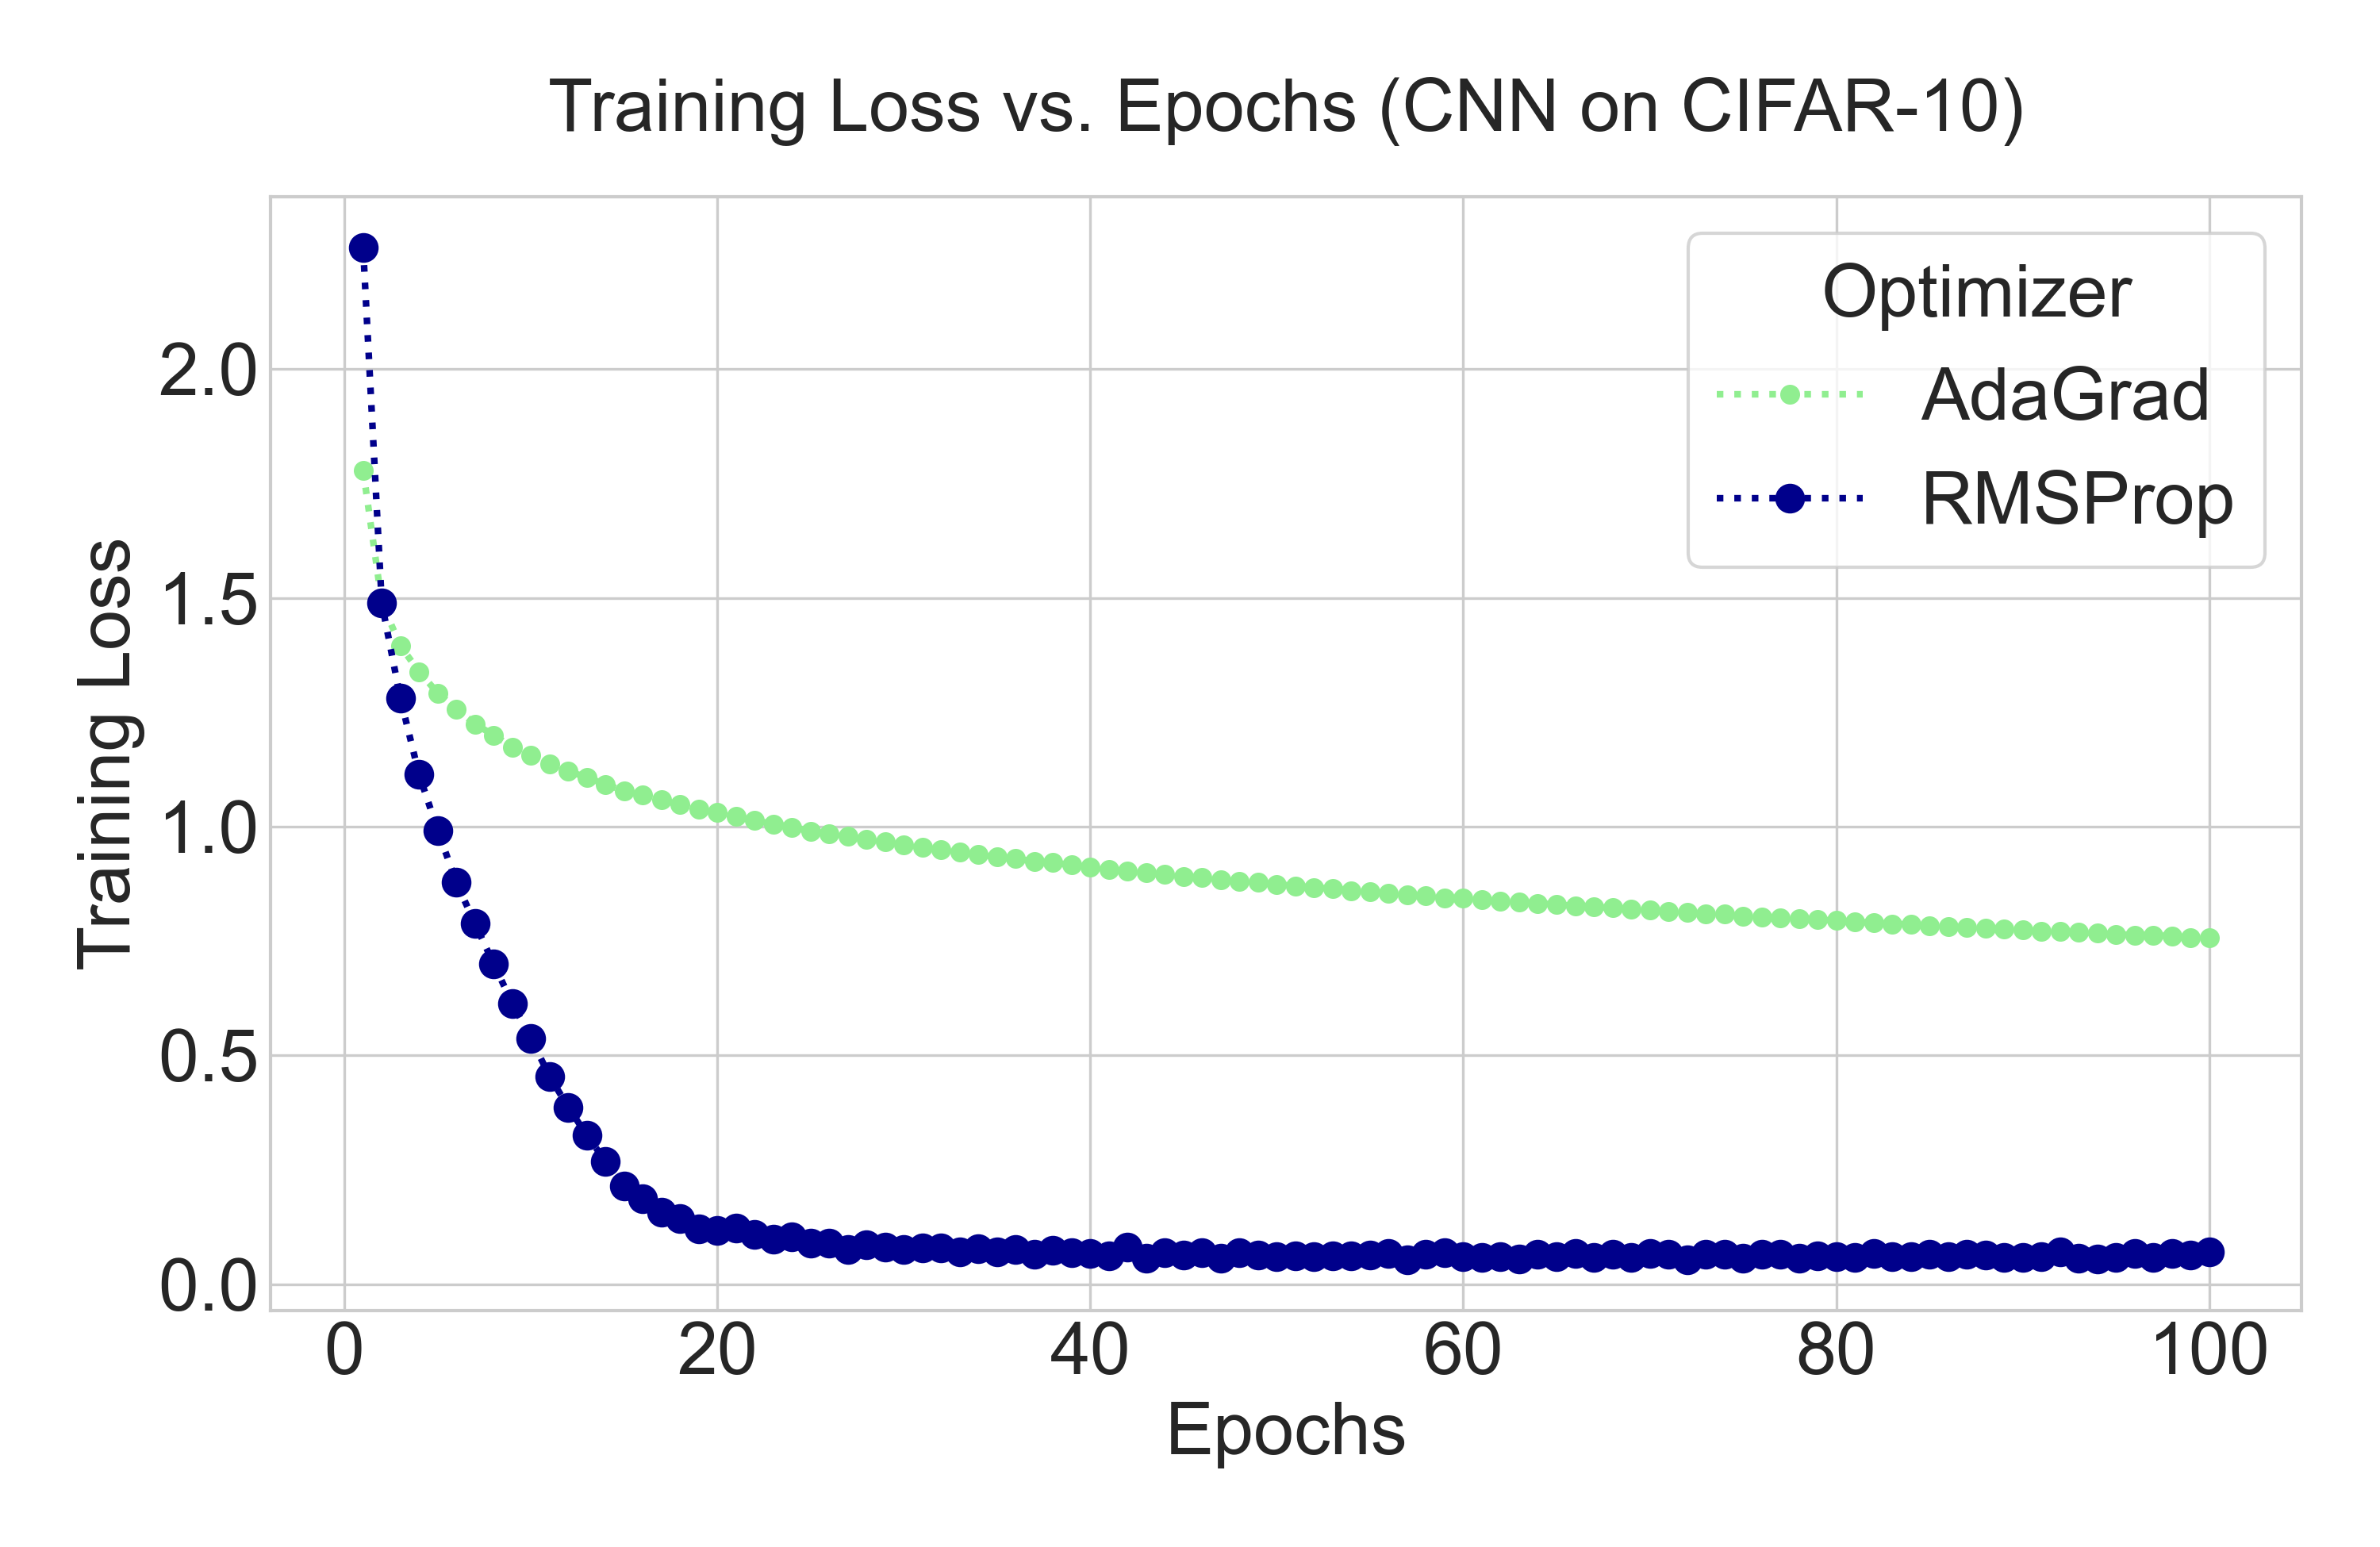
\includegraphics[width=0.48\textwidth]{Analysis_2_Impact_of_EMA2_cifar10_cnn_training_loss.png}} \quad
    \subfloat[CNN Accuracy on CIFAR-10]{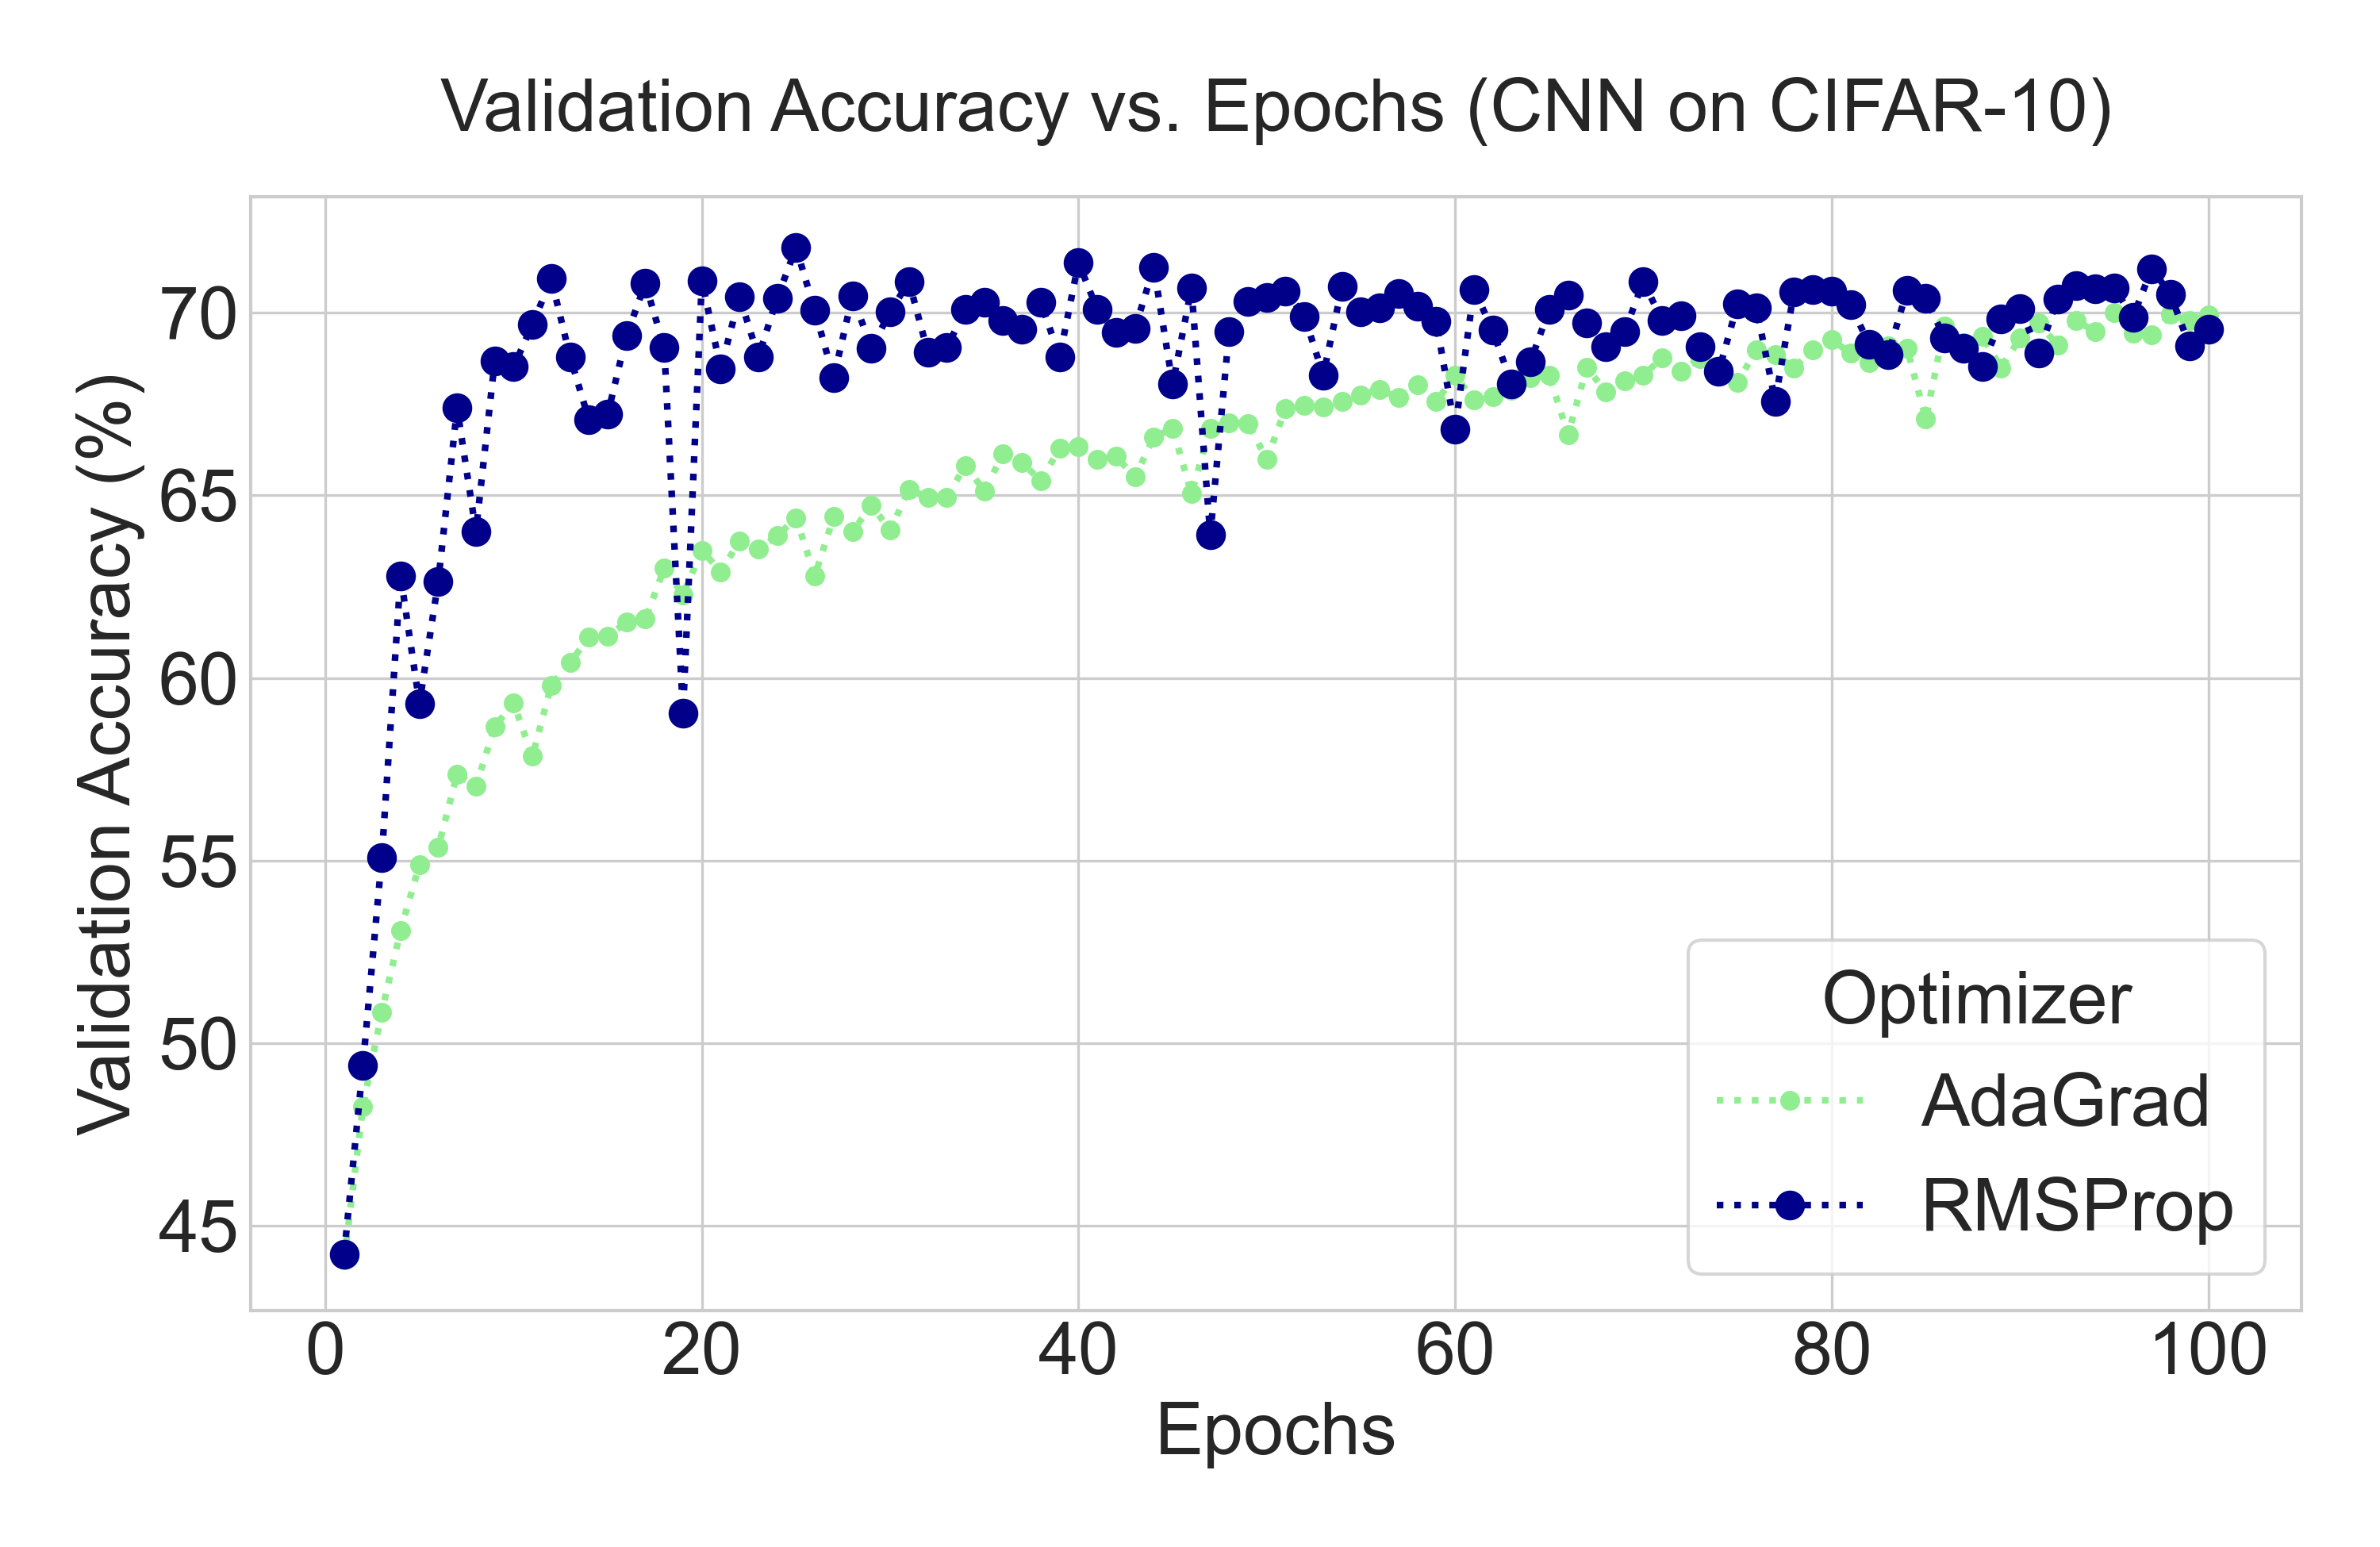
\includegraphics[width=0.48\textwidth]{Analysis_2_Impact_of_EMA2_cifar10_cnn_validation_accuracy.png}} \\
    % VGG13 row
    \subfloat[VGG13 Loss on CIFAR-10]{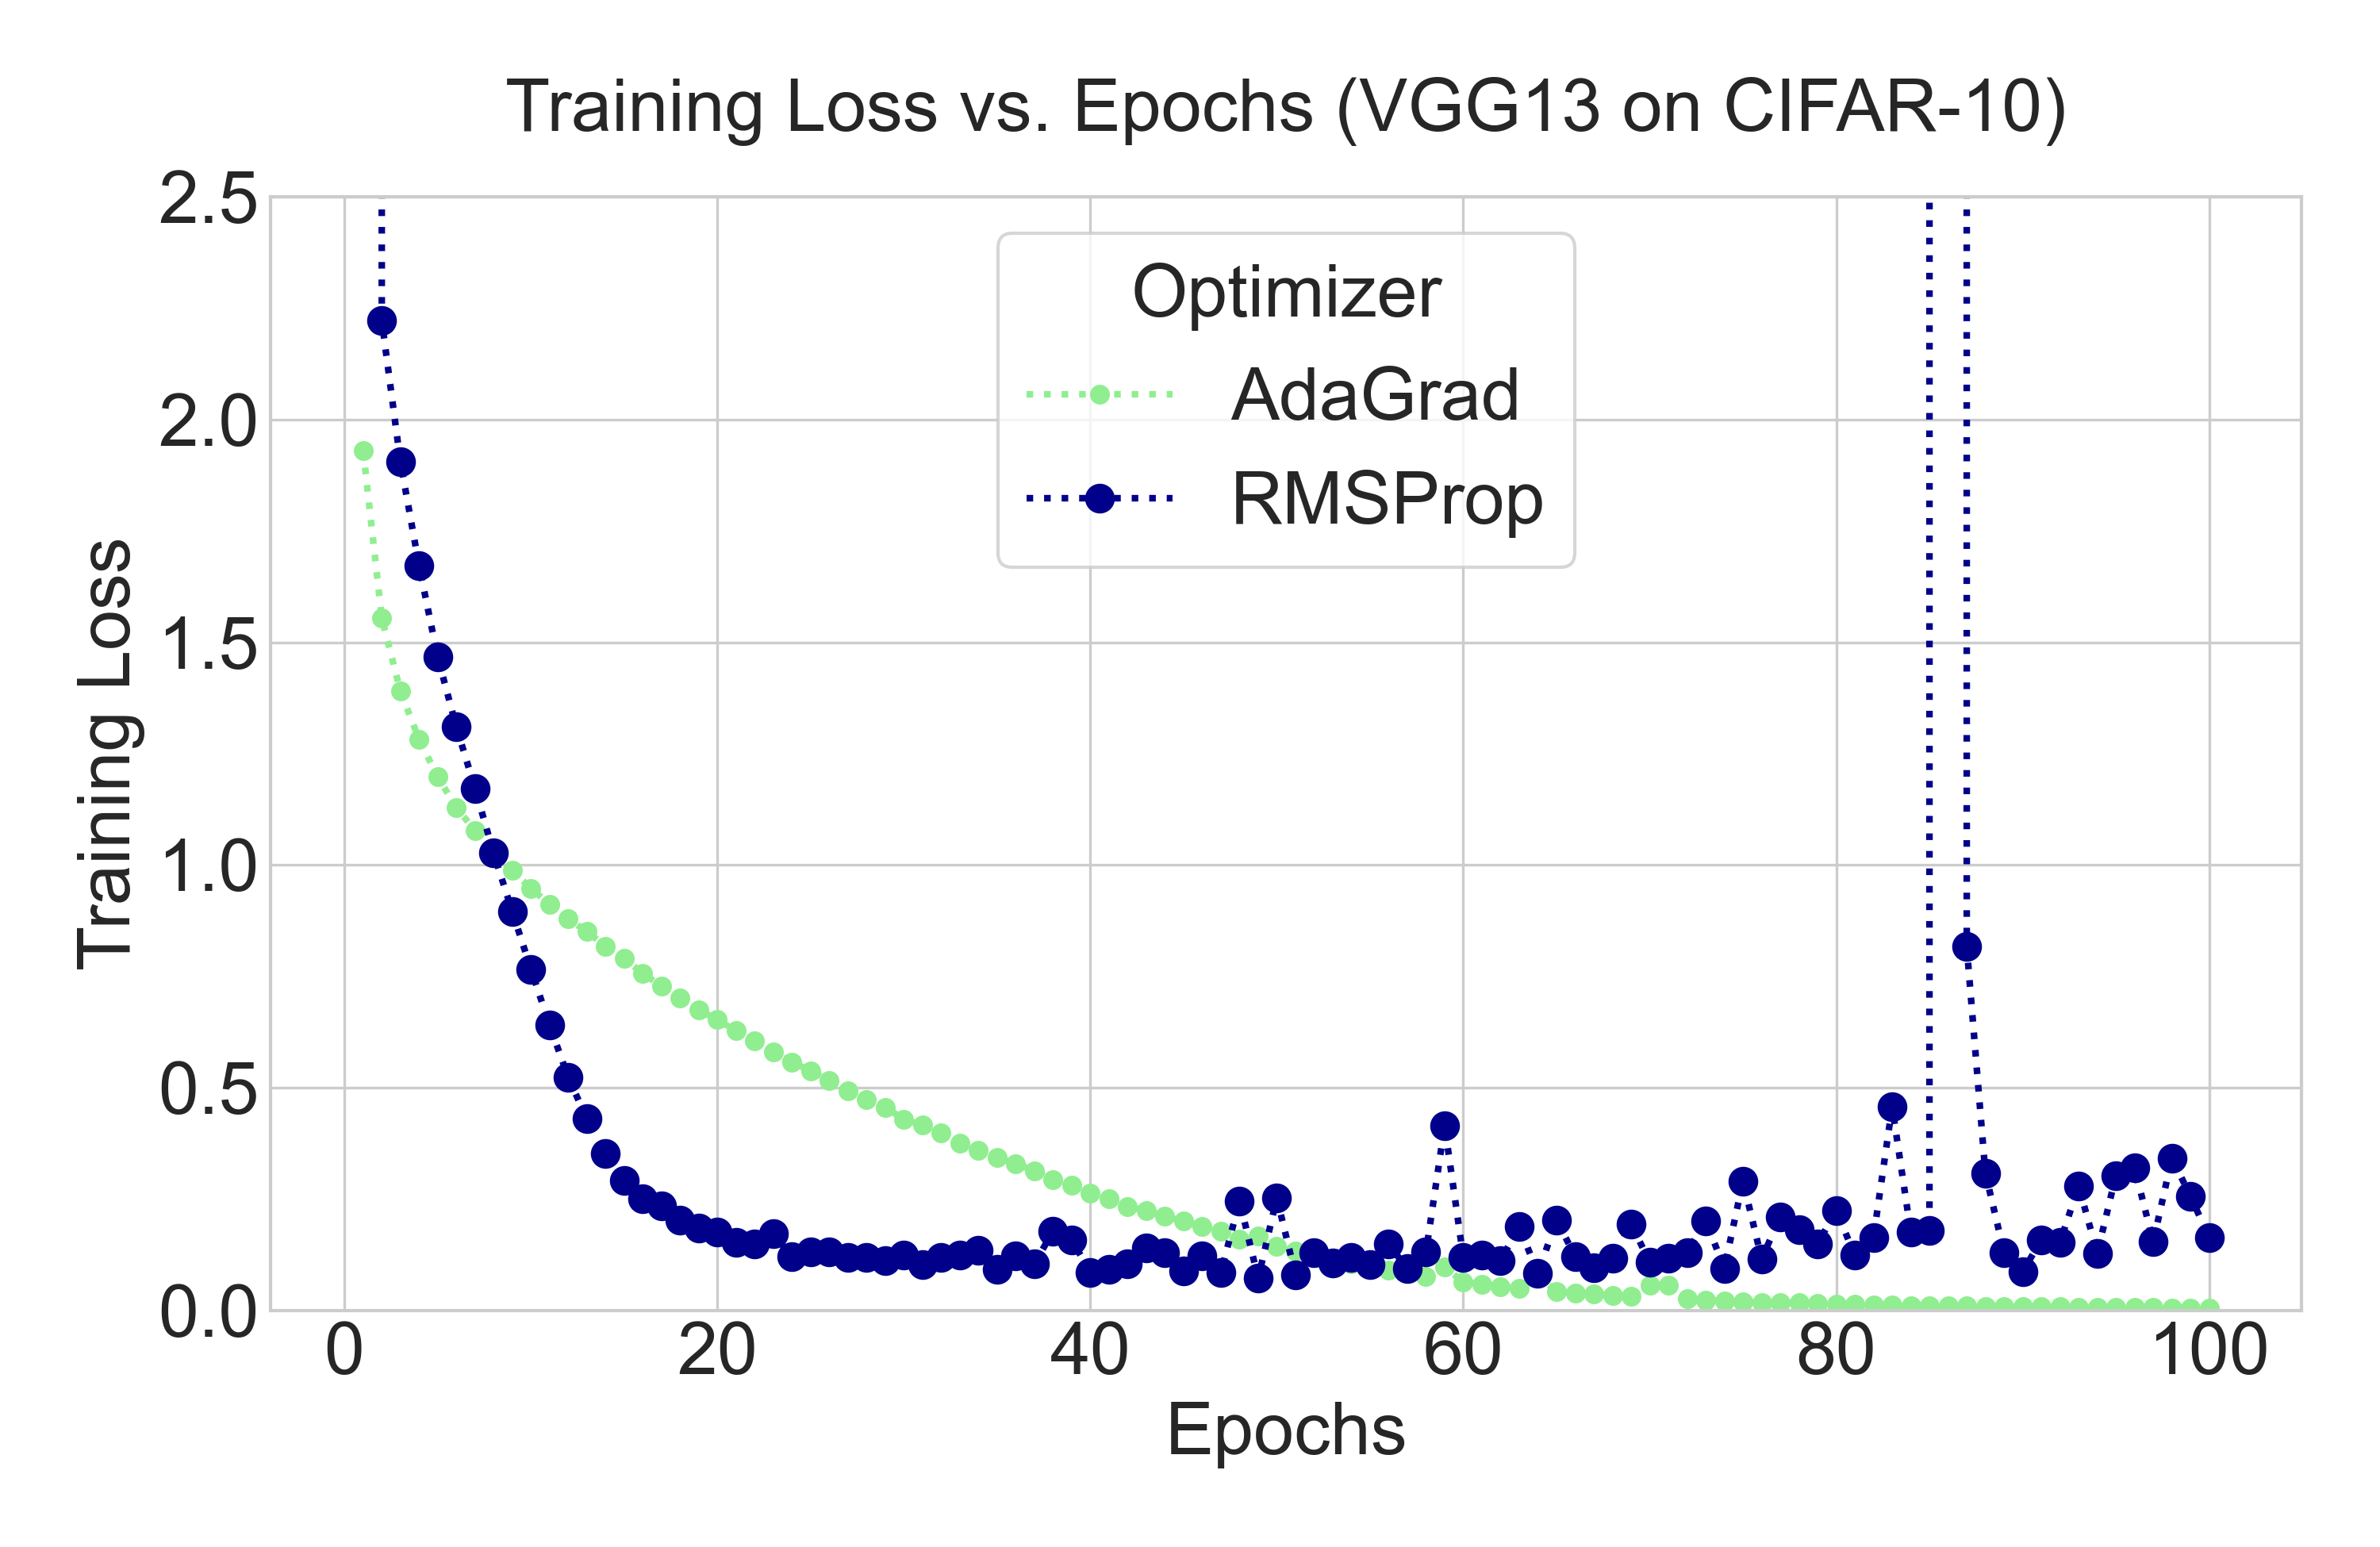
\includegraphics[width=0.48\textwidth]{Analysis_2_Impact_of_EMA3_cifar_vgg13_training_loss.png}} \quad
    \subfloat[VGG13 Accuracy on CIFAR-10]{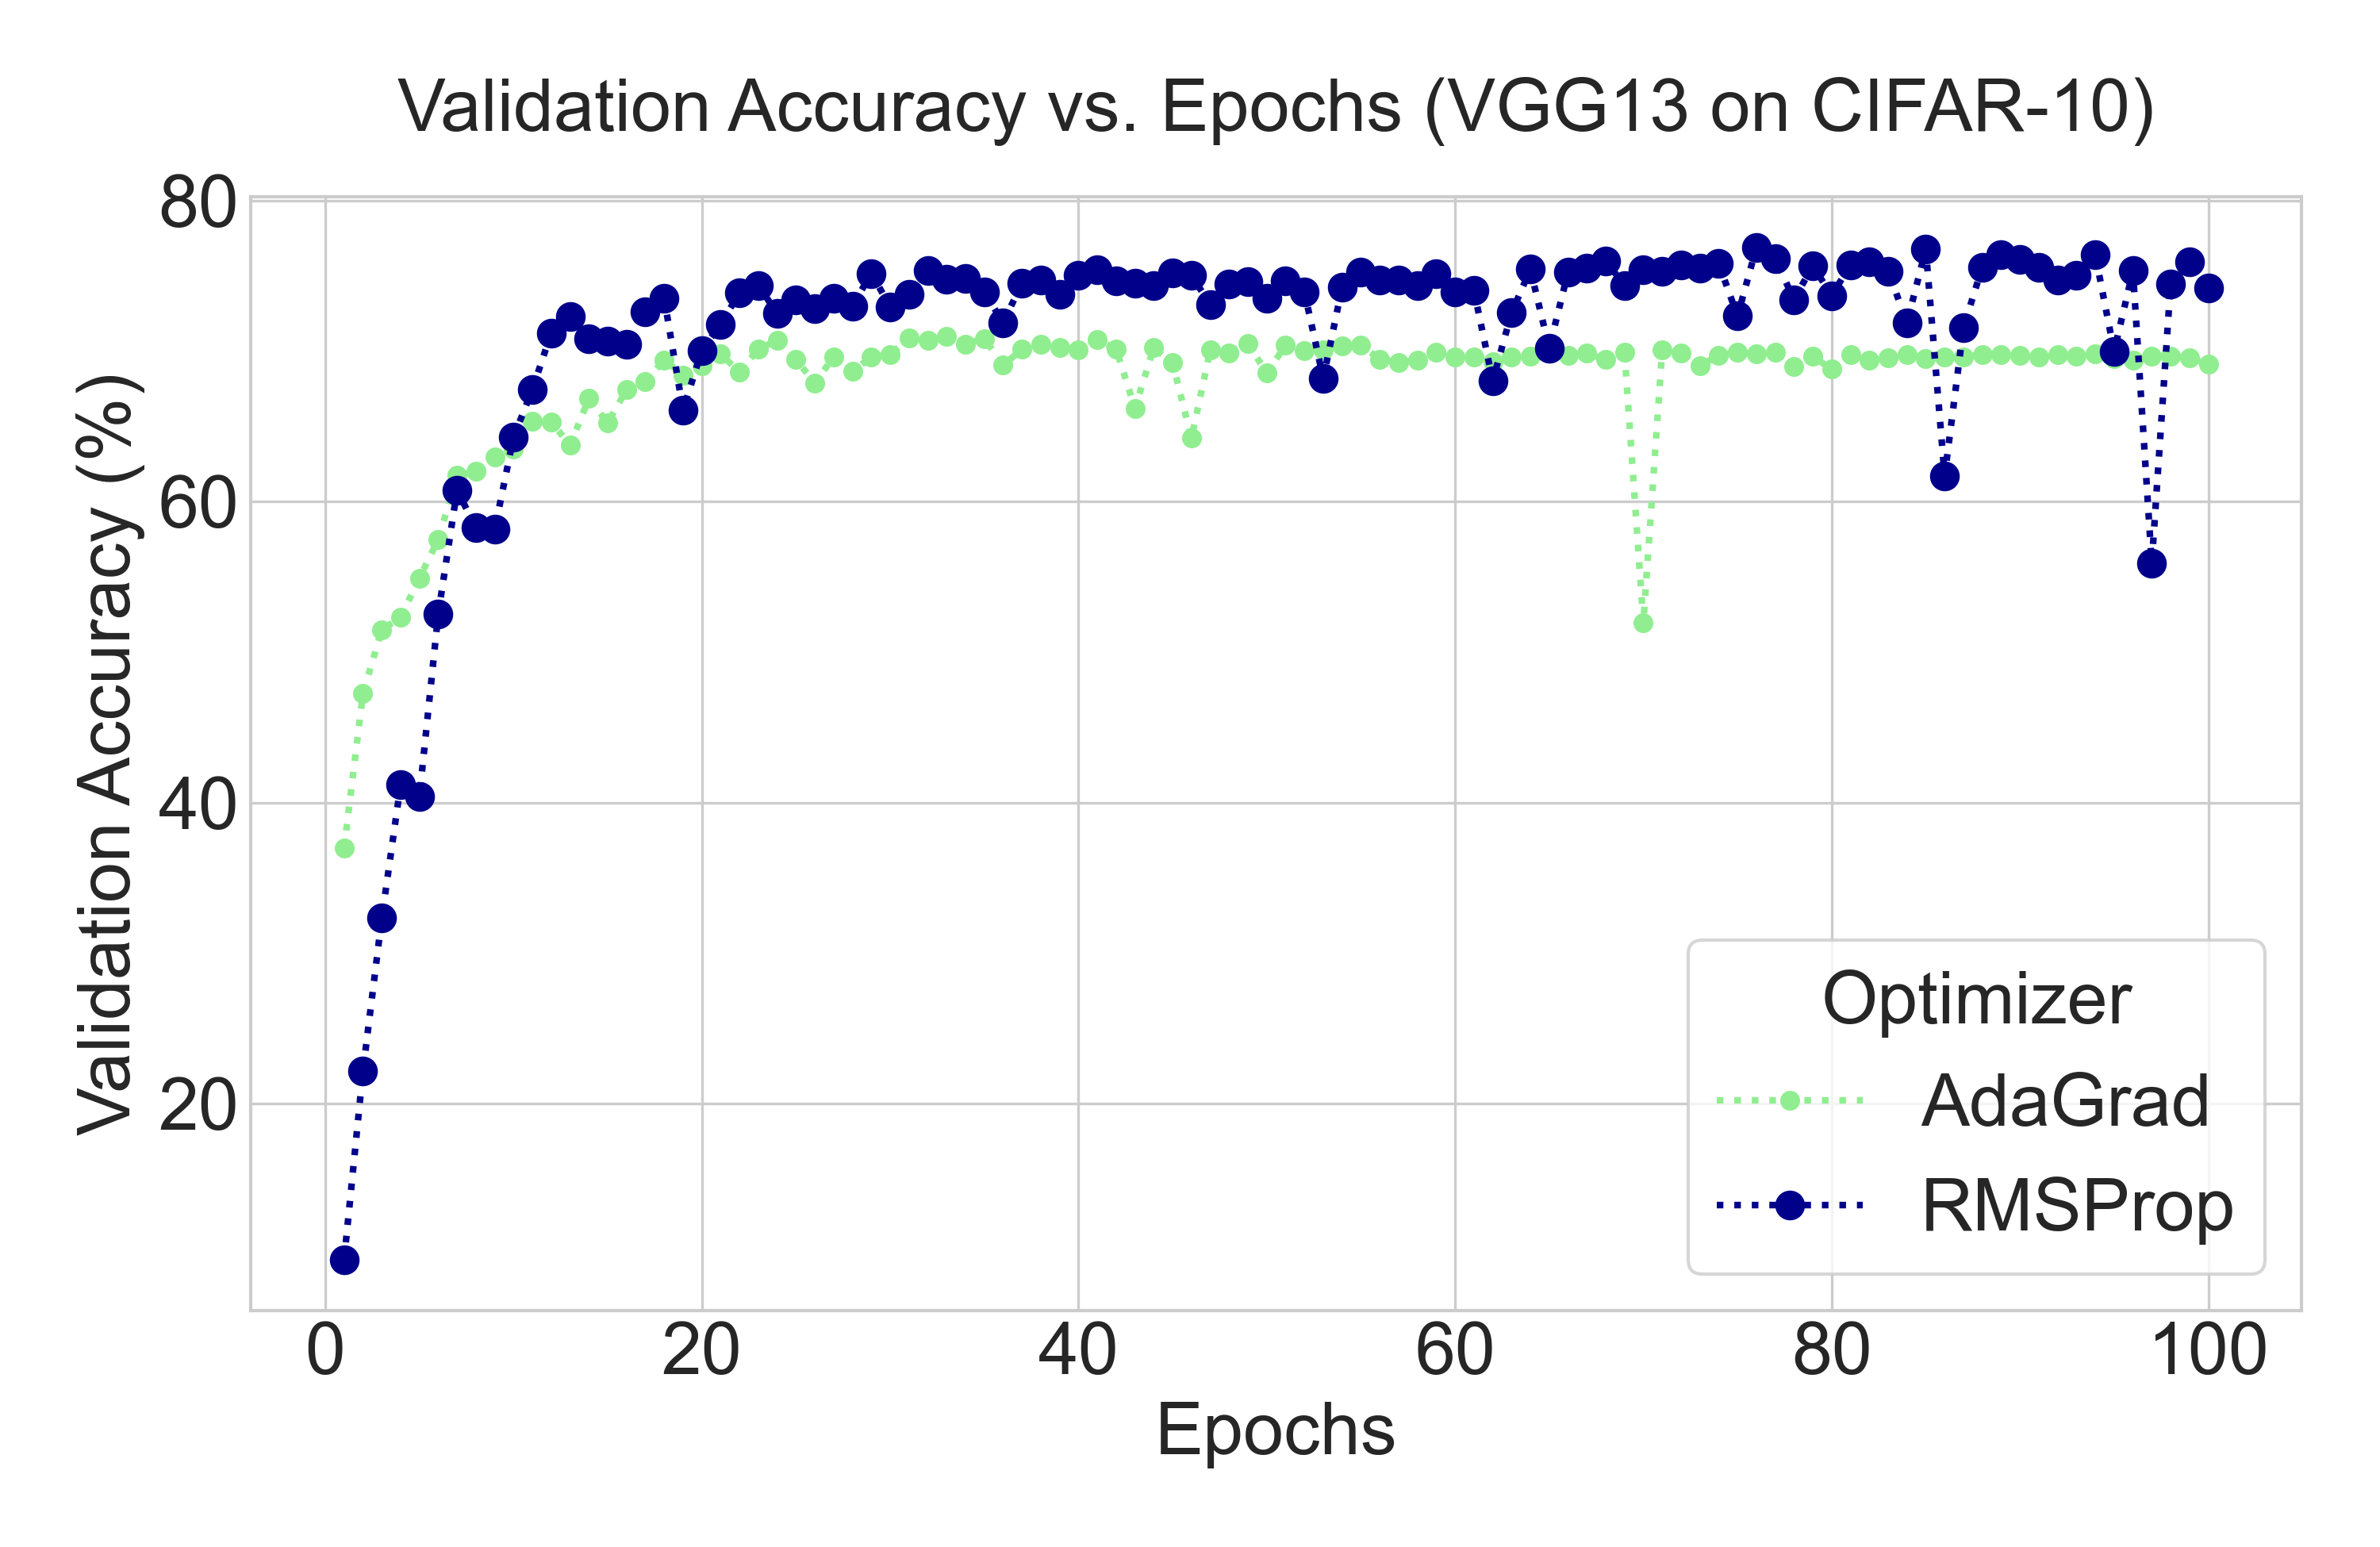
\includegraphics[width=0.48\textwidth]{Analysis_2_Impact_of_EMA3_cifar_vgg13_validation_accuracy.png}}
    \caption{Impact of exponential moving average: baseline method (AdaGrad, green line) vs. baseline method with exponential moving average (RMSProp, blue line)}
    \label{fig:comprehensive_comparison}
\end{figure}

\begin{table}[H]
\centering
\caption{Final Test Accuracy (RMSProp vs. AdaGrad)}
\label{tab:rmsprop_vs_adagrad}
\begin{tabular}{|l|c|c|c|}
\hline
        & MLP on MNIST & CNN on CIFAR-10 & VGG13 on CIFAR-10 \\ \hline
AdaGrad & 97.77\%      & \textbf{69.98\%}  & 68.11\%           \\ \hline
RMSProp & \textbf{98.29\%} & 68.65\%         & \textbf{73.61\%}    \\ \hline
\end{tabular}
\end{table}

From Experiment.2, we can generally observe that RMSProp performs better than AdaGrad overall. However, in the final test accuracy, AdaGrad performs slightly better in the CNN on CIFAR-10 experiment. RMSProp introduces an Exponential Moving Average, but in essence, both RMSProp and AdaGrad improve gradient descent through adaptive learning rates.

Looking at the training loss curves, \textbf{RMSProp shows a faster convergence speed.} During the first 0–20 epochs, the RMSProp curve drops more steeply. In terms of training speed, RMSProp reaches a stable accuracy within about 20 epochs, which means it converges faster.

From the graphs, we can also see that \textbf{RMSProp has much more fluctuation.} In Figures b, d, e, and f, the RMSProp curves oscillate more than those of AdaGrad. In Figure e, RMSProp even produces an almost infinitely large loss value. 

Both AdaGrad and RMSProp follow the idea of adaptive gradients, but their update methods differ. AdaGrad accumulates the squared gradients for each parameter over time, which acts as a form of long-term memory. RMSProp, on the other hand, reduces the influence of older gradients by using exponential decay. \textbf{This adjustment allows RMSProp to perform better in some cases but also makes it more sensitive to sudden large gradients.} Because RMSProp gives higher weight to recent gradients, it is more prone to extreme fluctuations. As seen in the plots, RMSProp shows near-infinite values, which do not occur in AdaGrad.

Overall, the difference in final accuracy between the two methods is small, with each performing better in different situations. \textbf{On the CIFAR-10 dataset, although AdaGrad performs better with a simple CNN, RMSProp achieves higher accuracy when using VGG13. This indicates that while RMSProp may experience occasional instability during training, it still demonstrates stronger generalization ability and better accuracy in more complex models.}


%--------------------------------------------
\subsection{Momentum}


\begin{figure}[htbp]
    \centering
    % MLP row
    \subfloat[MLP Loss on MNIST]{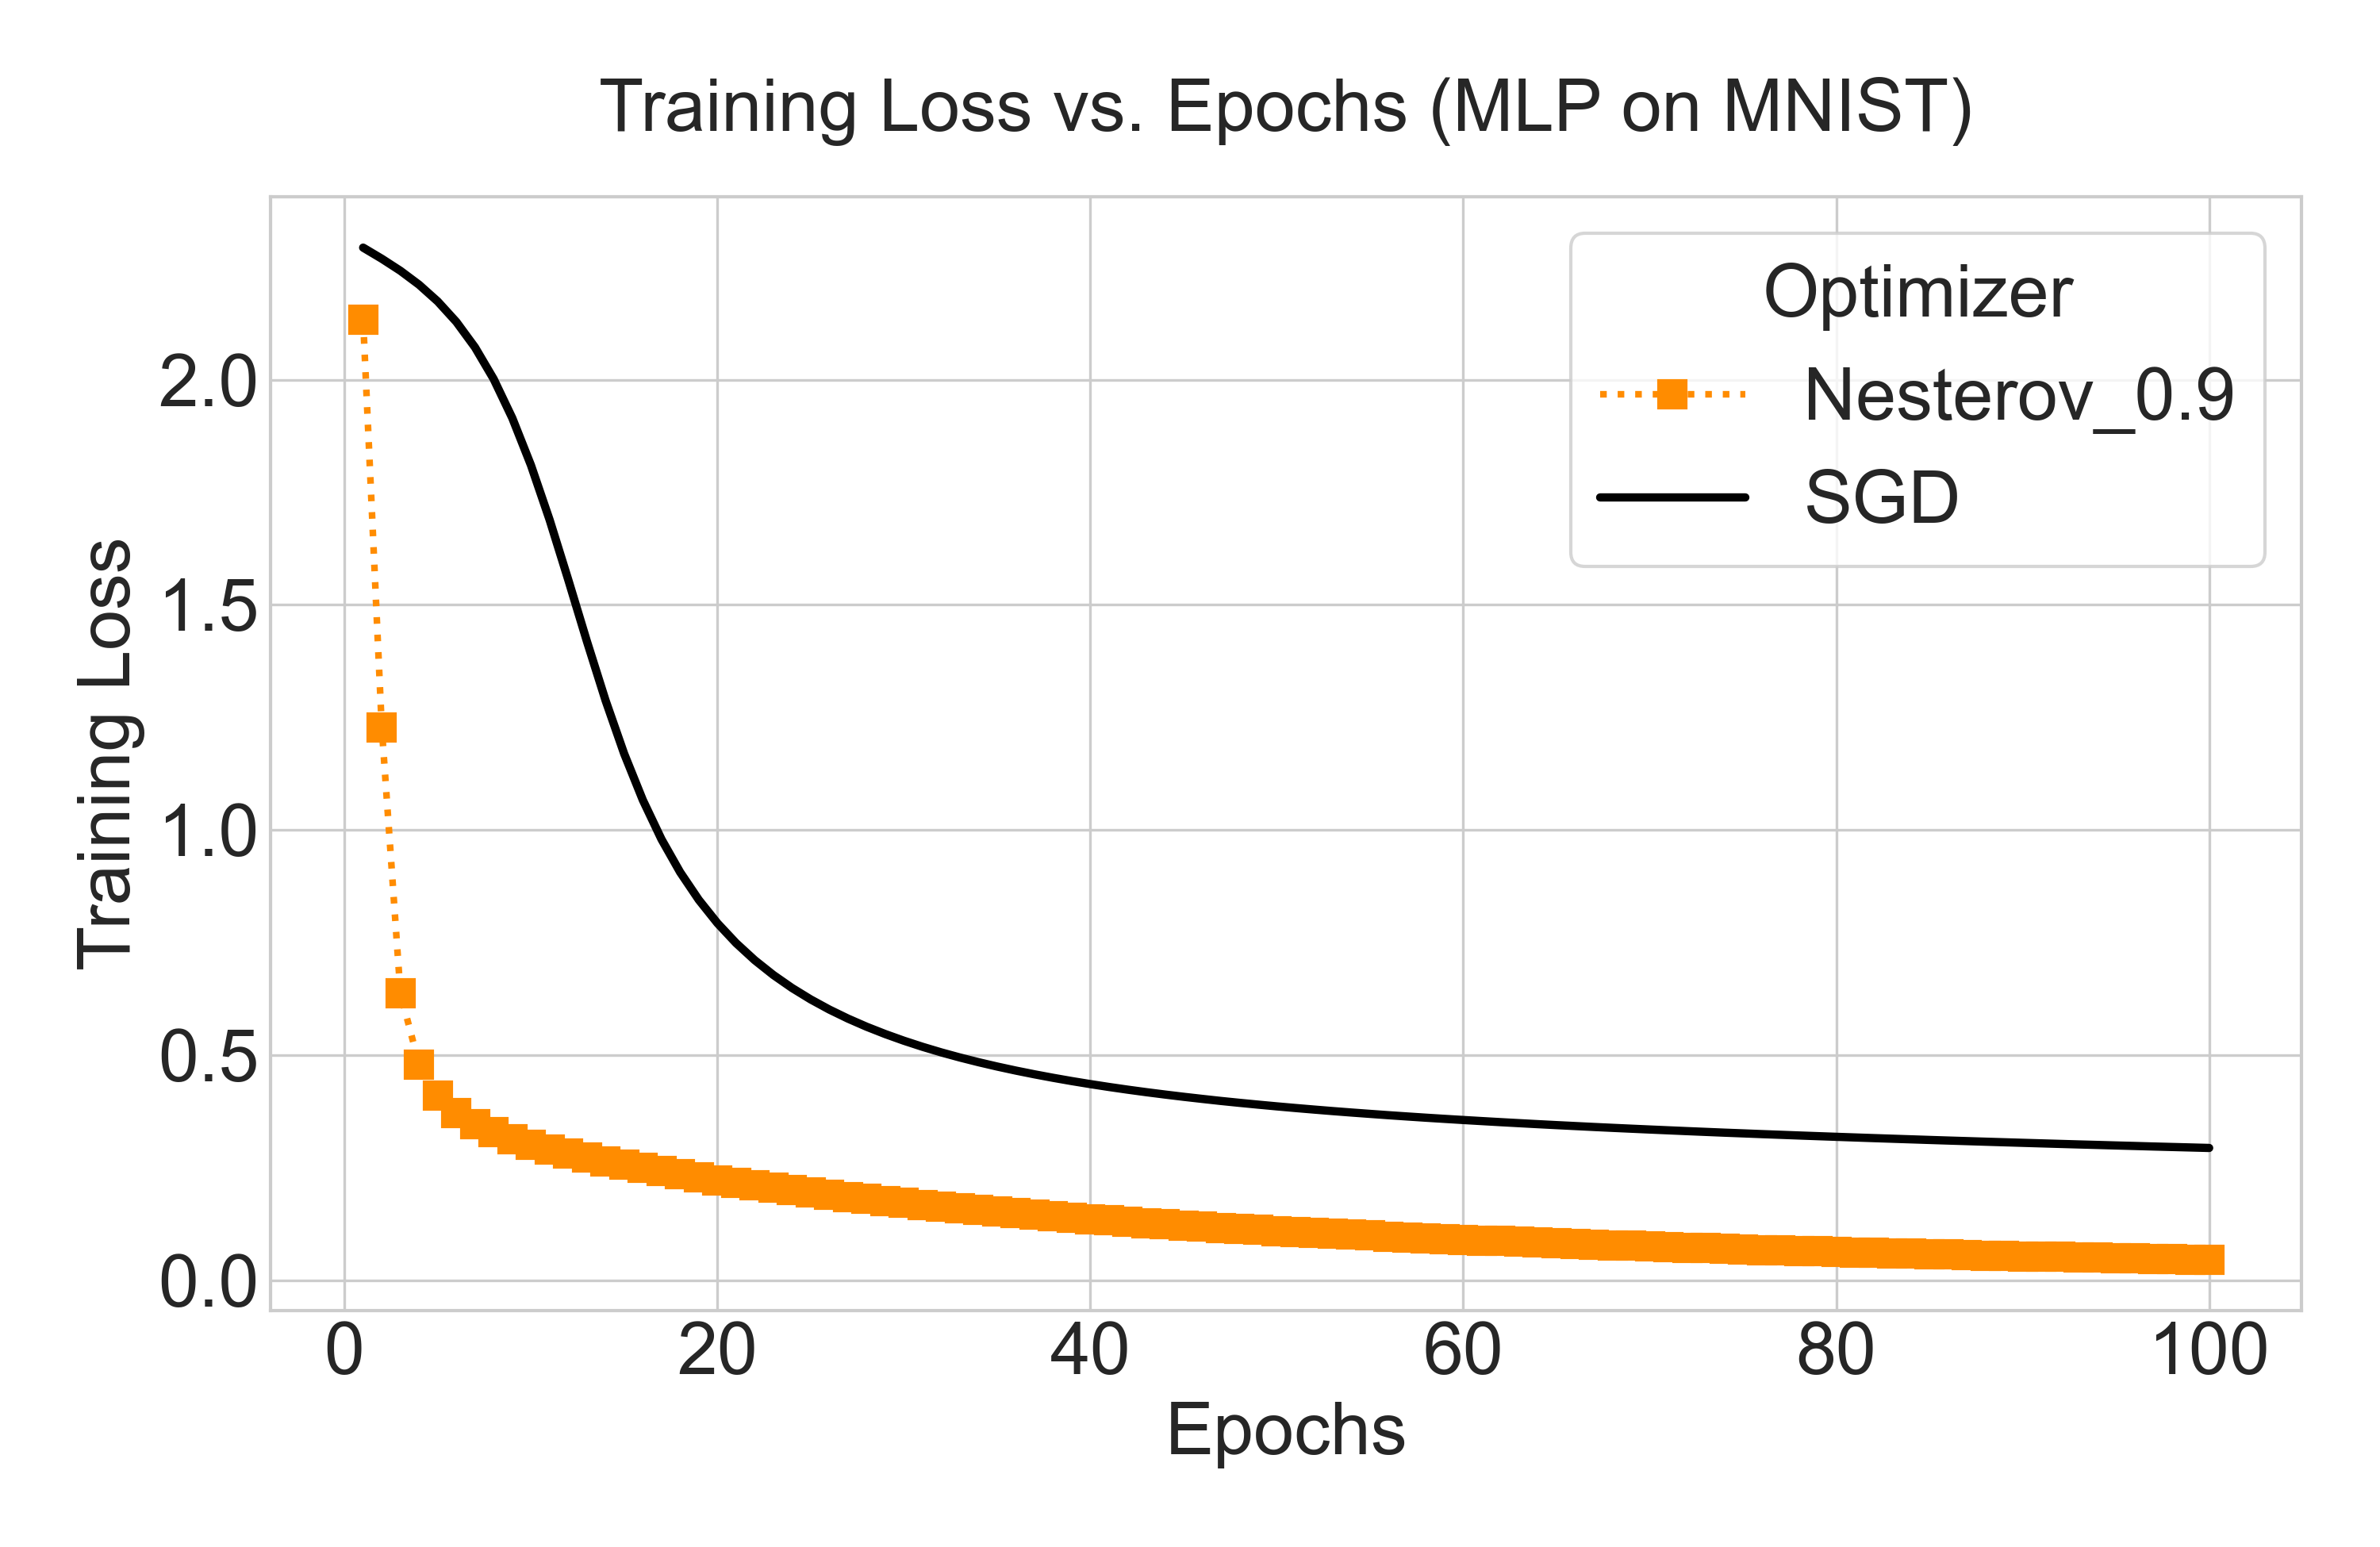
\includegraphics[width=0.48\textwidth]{Analysis_3_Impact_of_Momentum1_mnist_mlp_training_loss.png}} \quad
    \subfloat[MLP Accuracy on MNIST ]{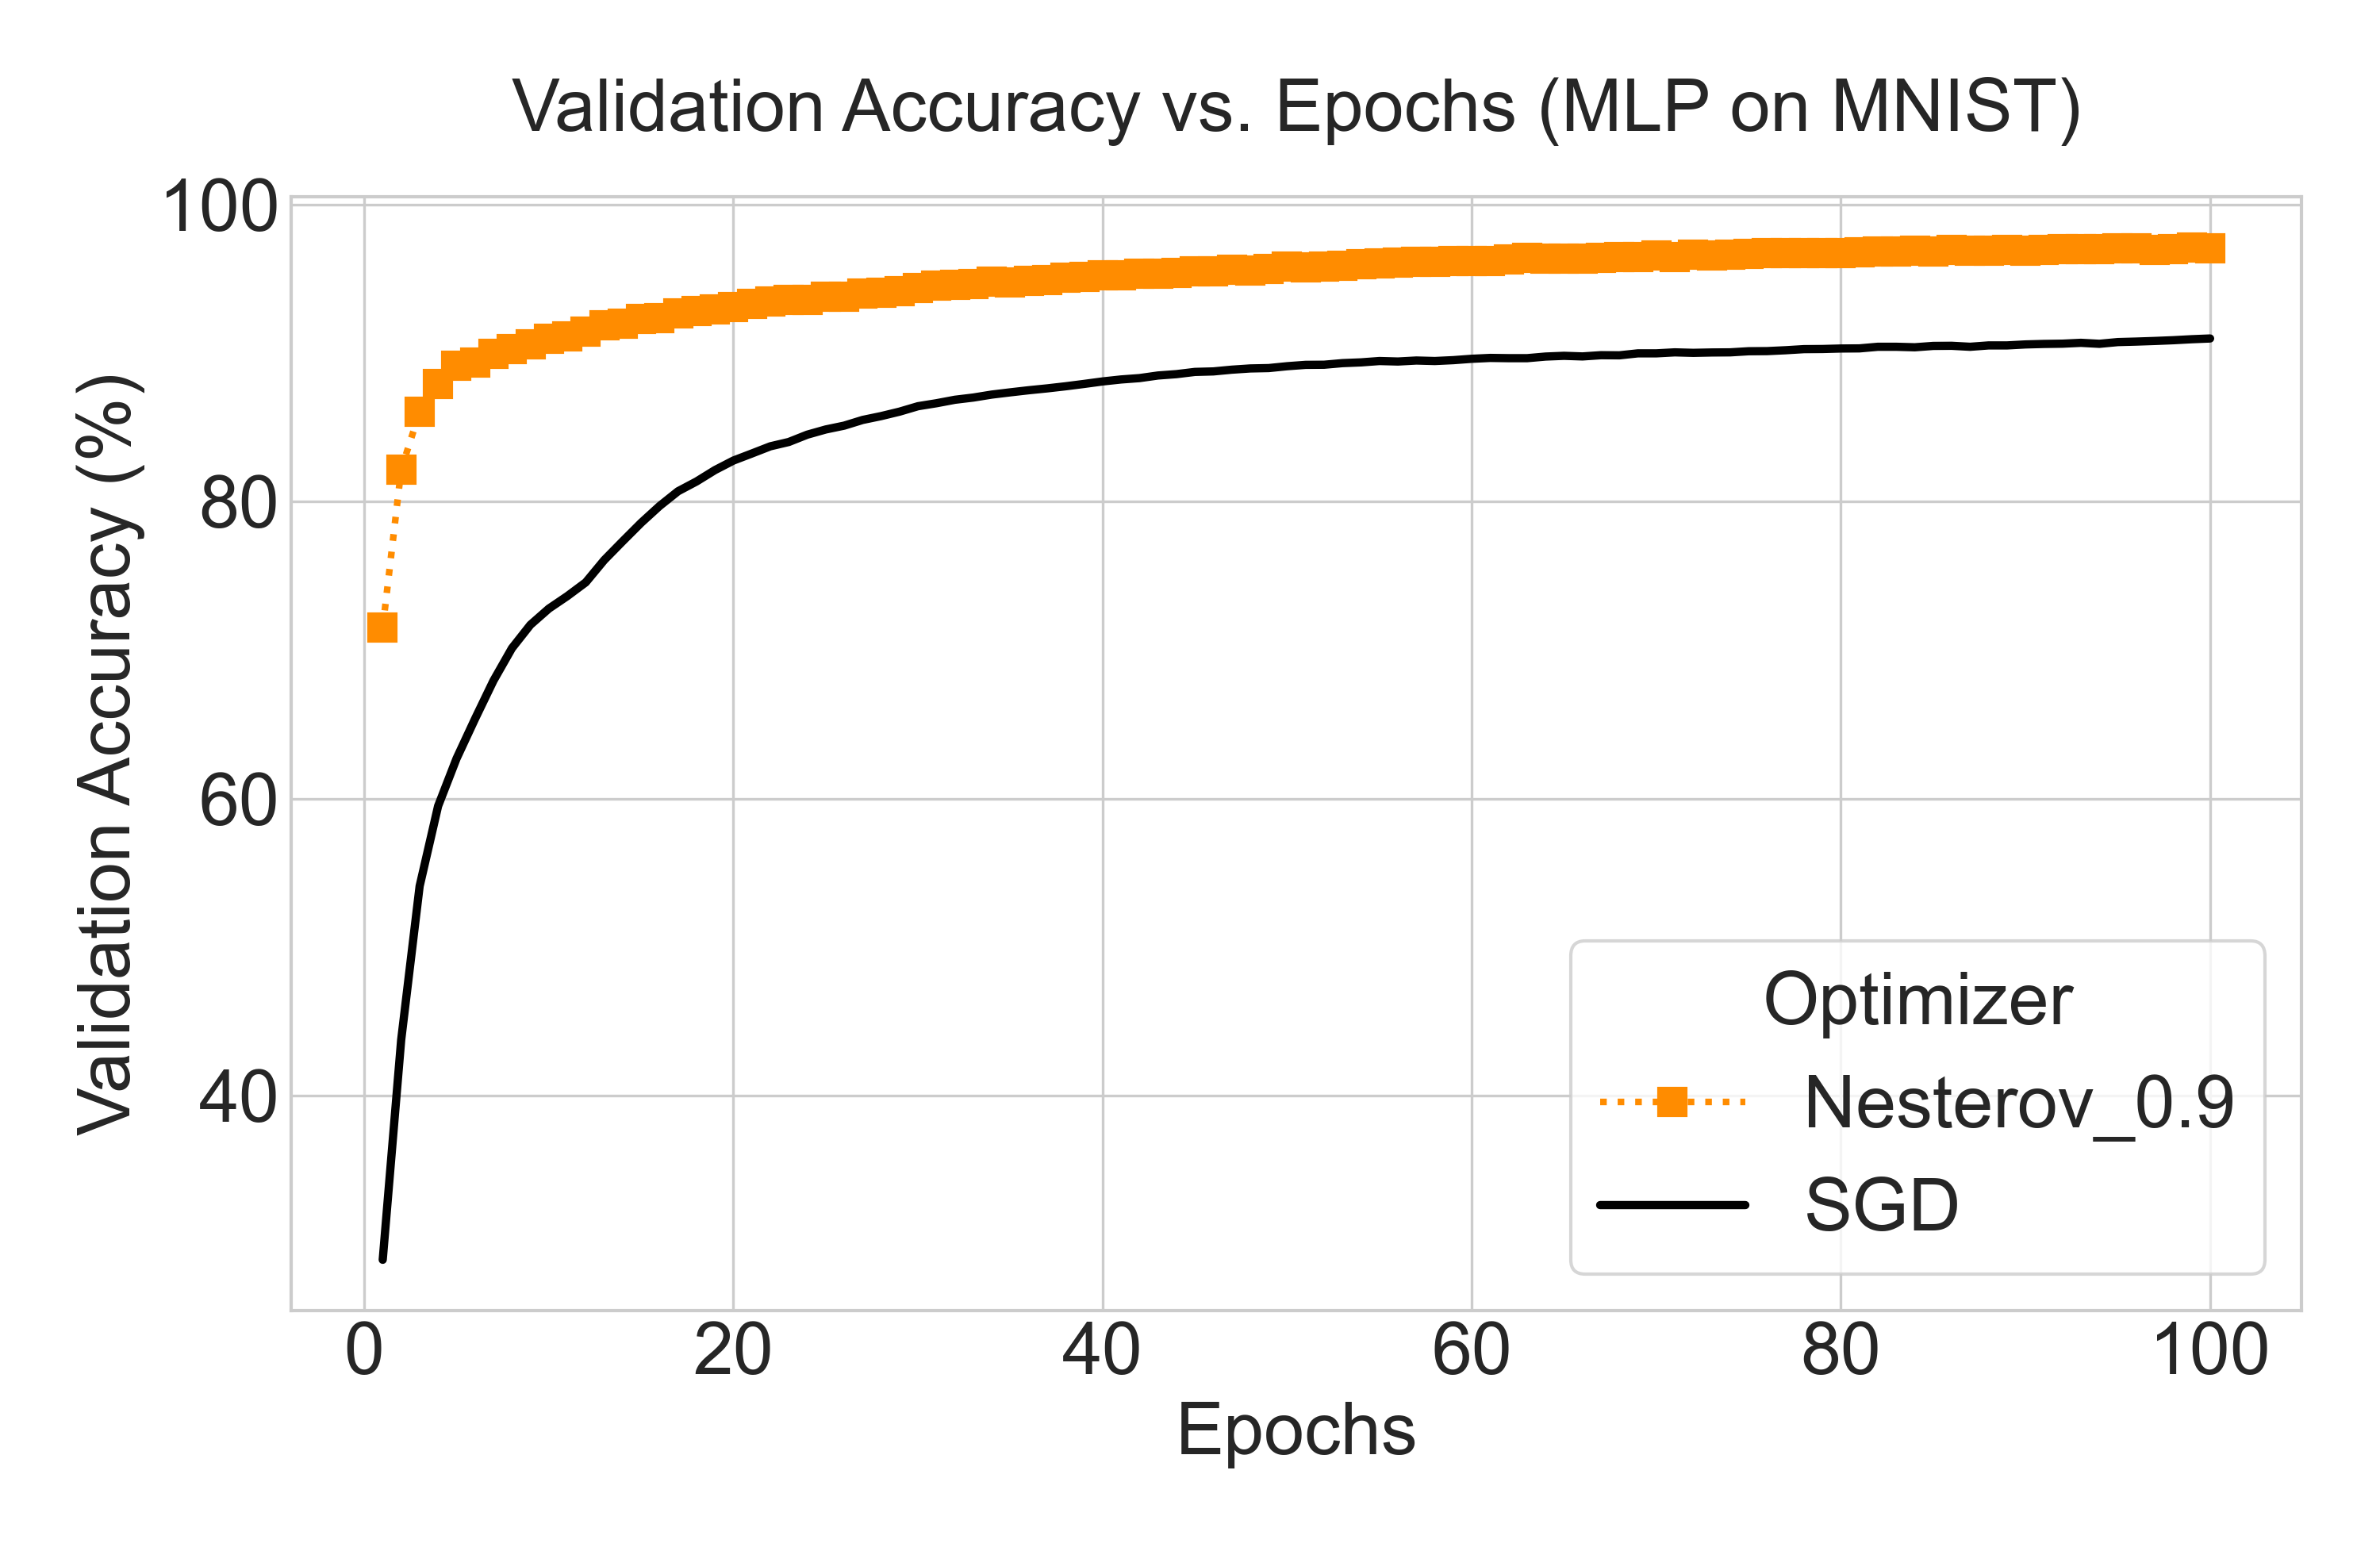
\includegraphics[width=0.48\textwidth]{Analysis_3_Impact_of_Momentum1_mnist_mlp_validation_accuracy.png}} \\
    % CNN row
    \subfloat[CNN Loss on CIFAR-10 ]{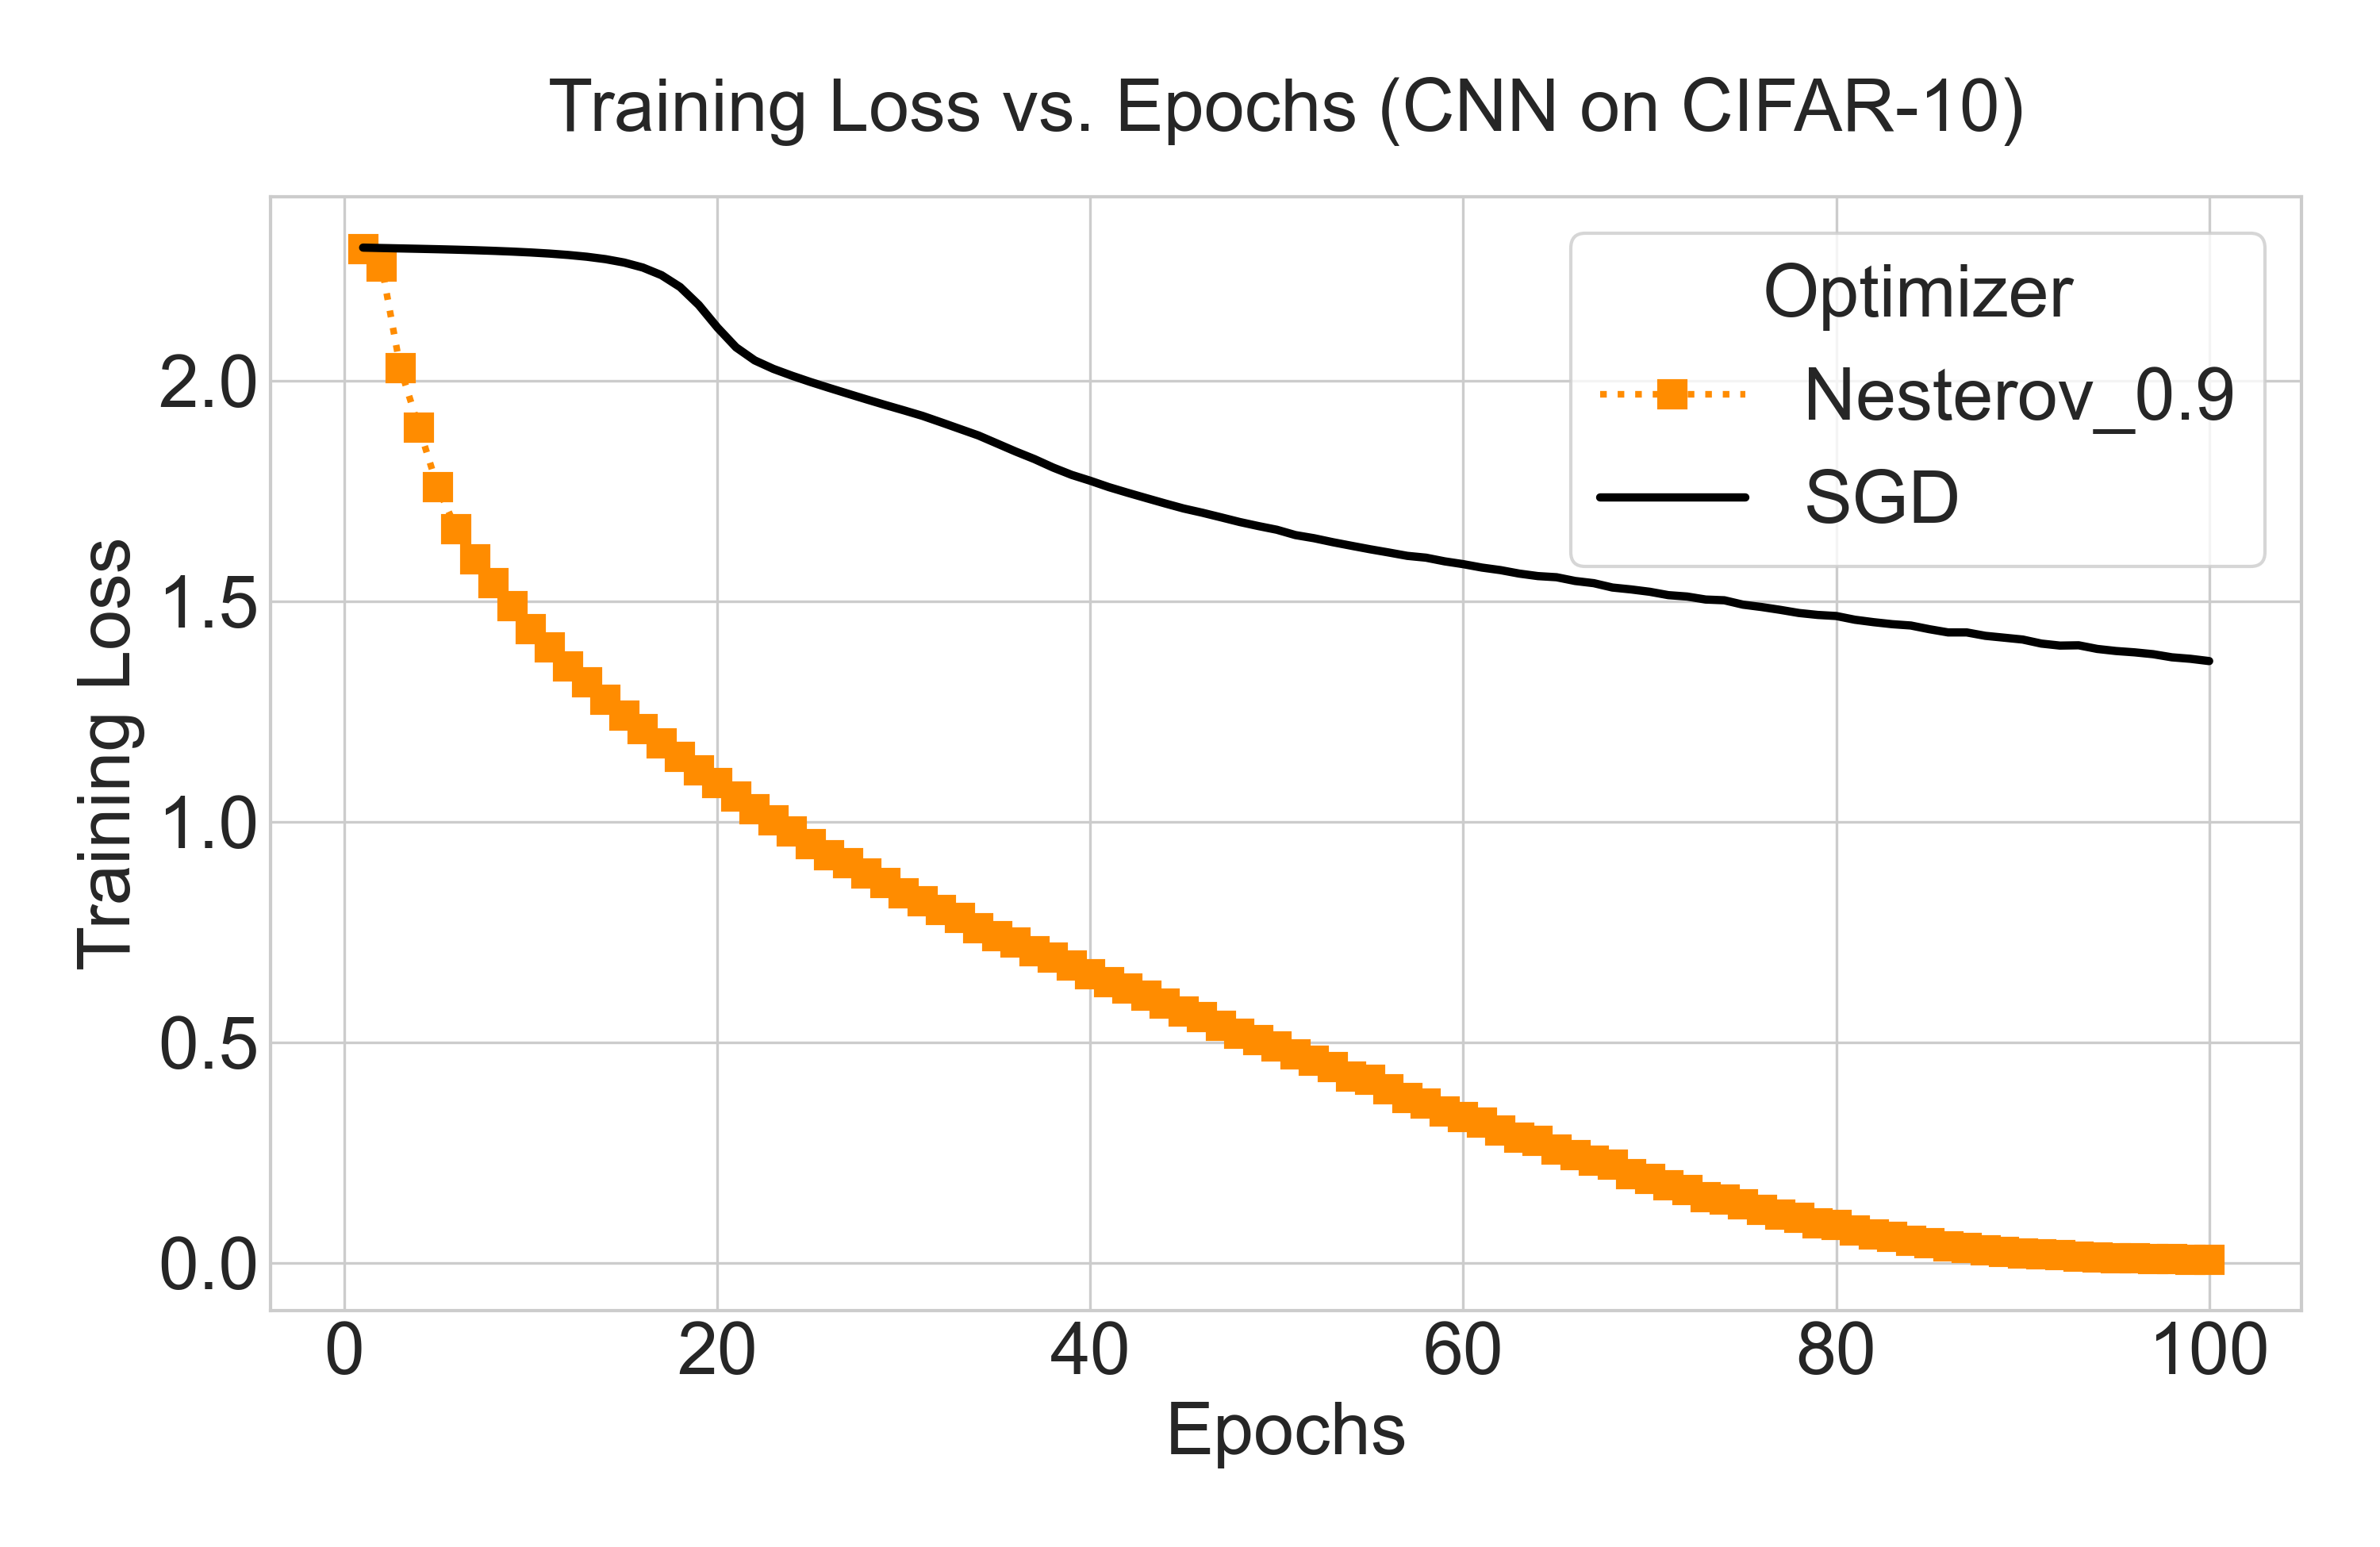
\includegraphics[width=0.48\textwidth]{Analysis_3_Impact_of_Momentum2_cifar10_cnn_training_loss.png}} \quad
    \subfloat[CNN Accuracy on CIFAR-10 ]{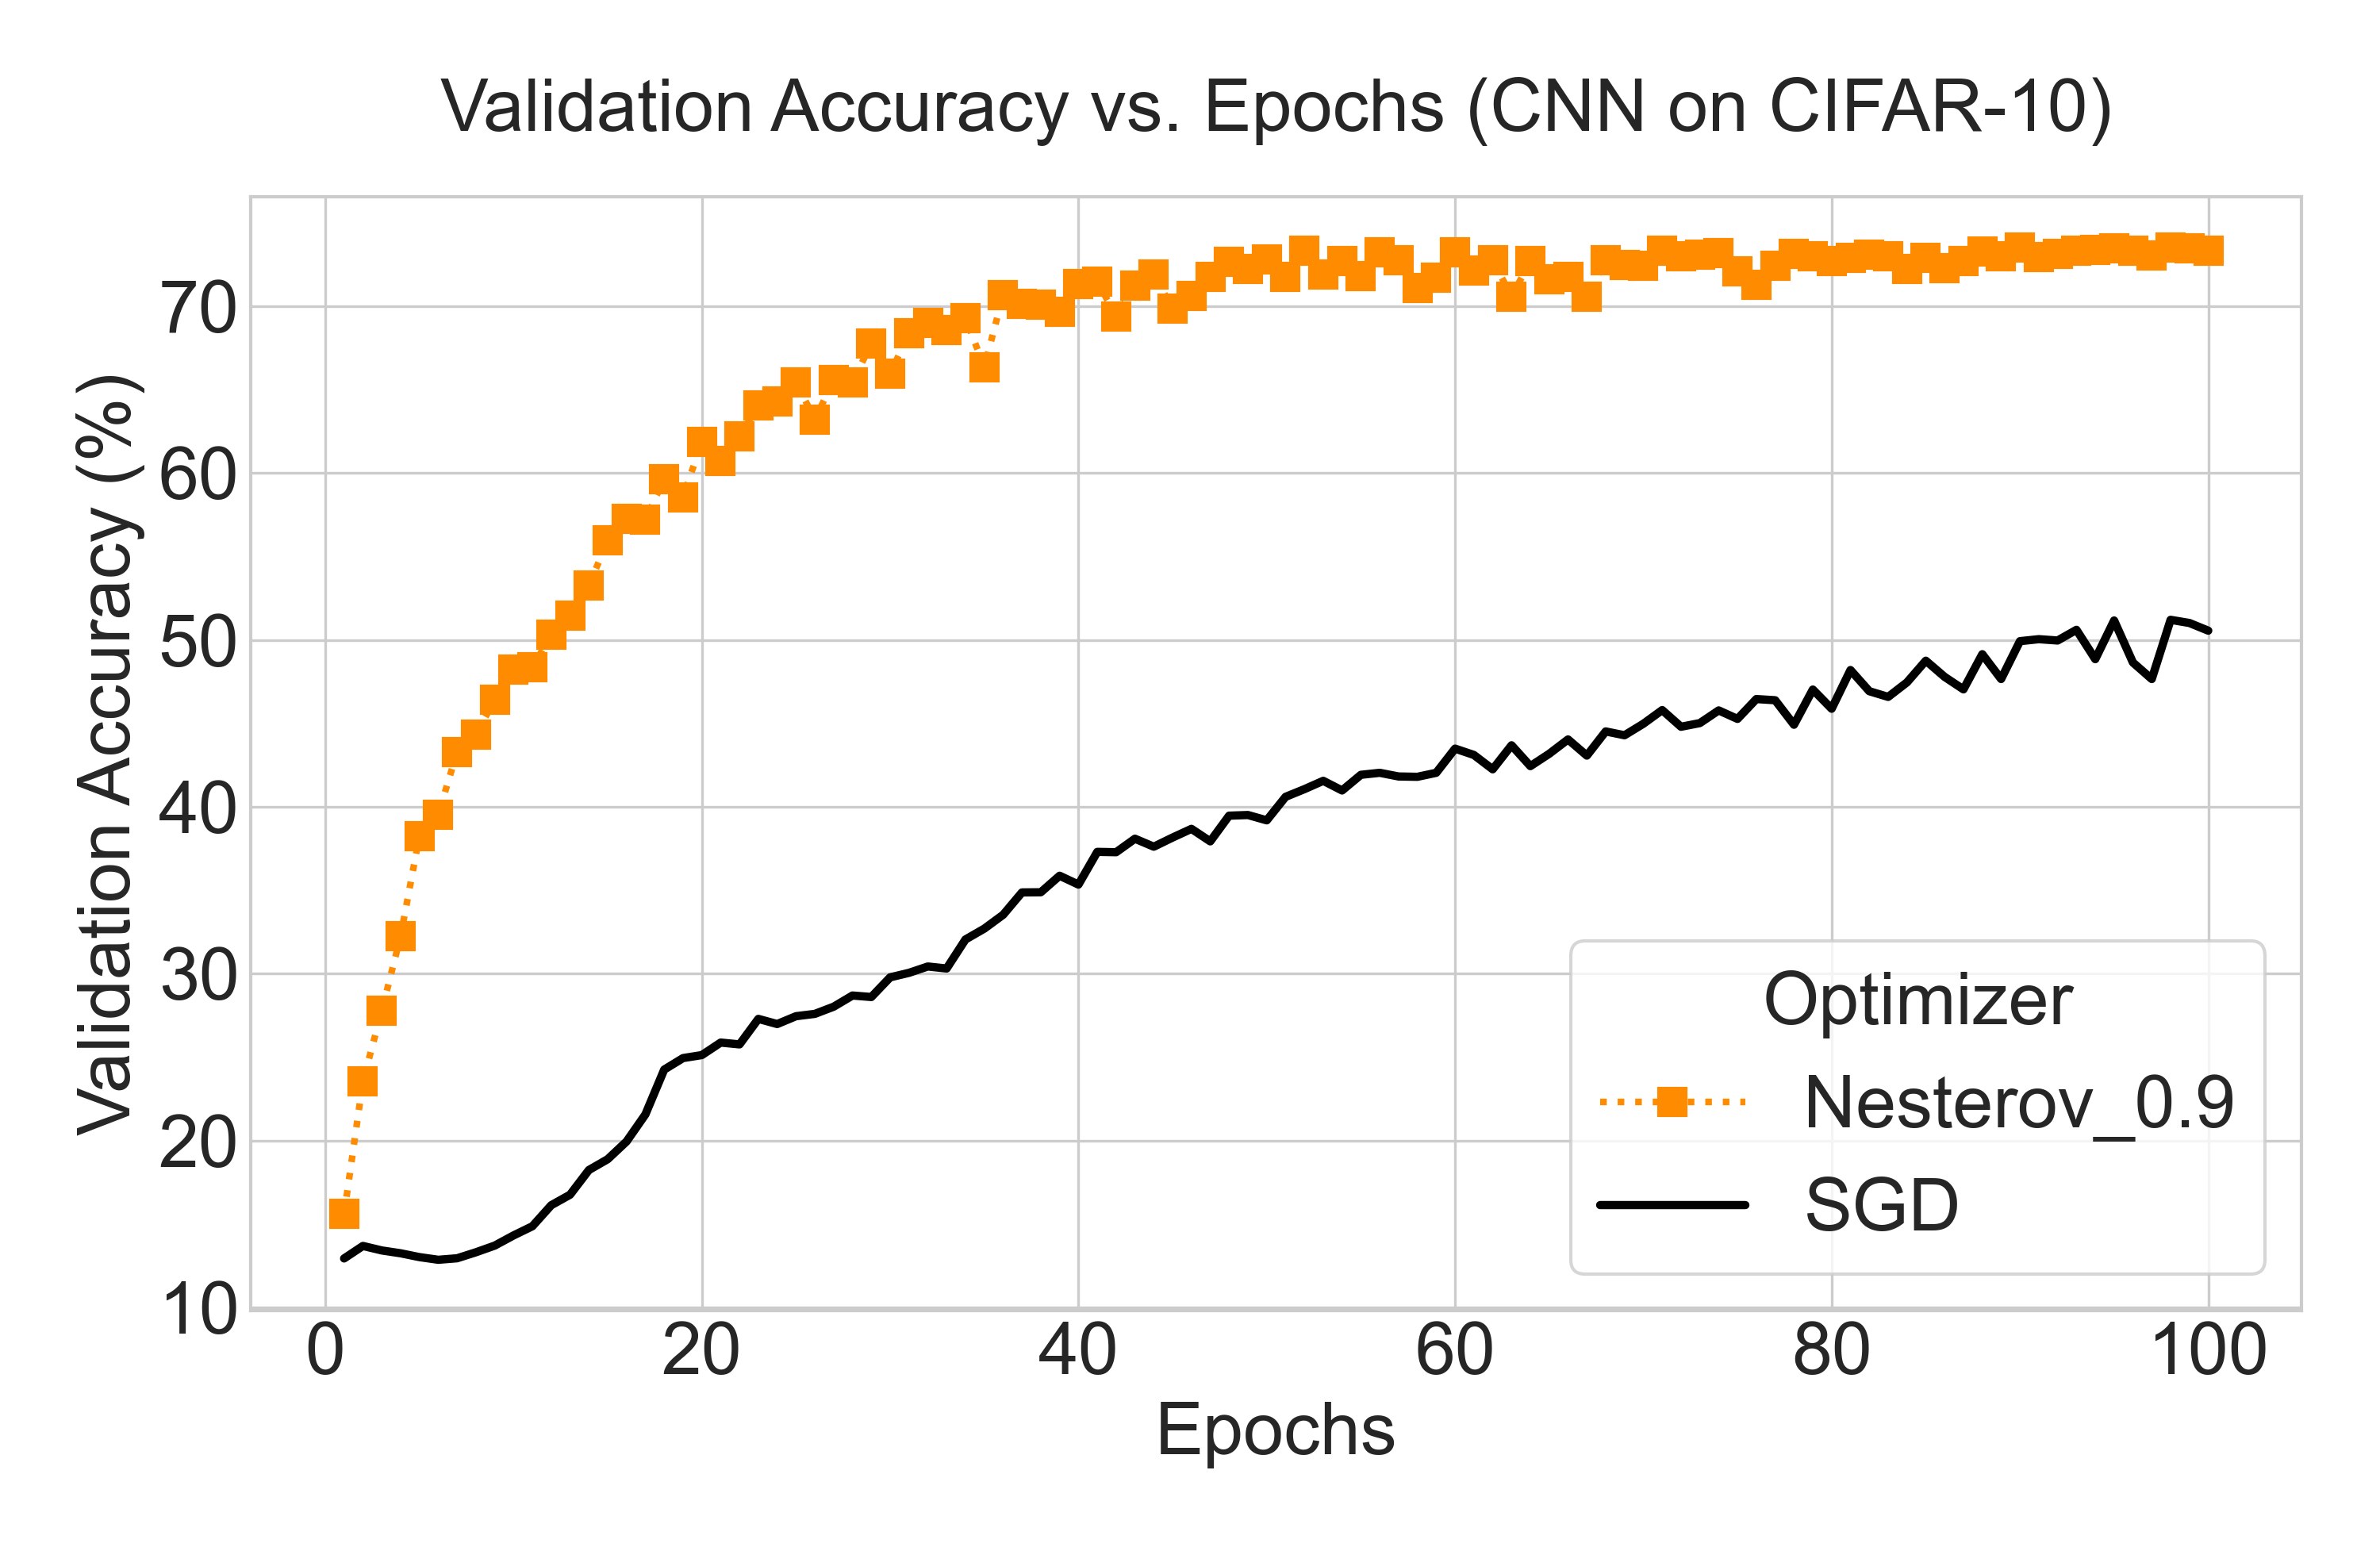
\includegraphics[width=0.48\textwidth]{Analysis_3_Impact_of_Momentum2_cifar10_cnn_validation_accuracy.png}} \\
    % VGG13 row
    \subfloat[VGG13 Loss on CIFAR-10]{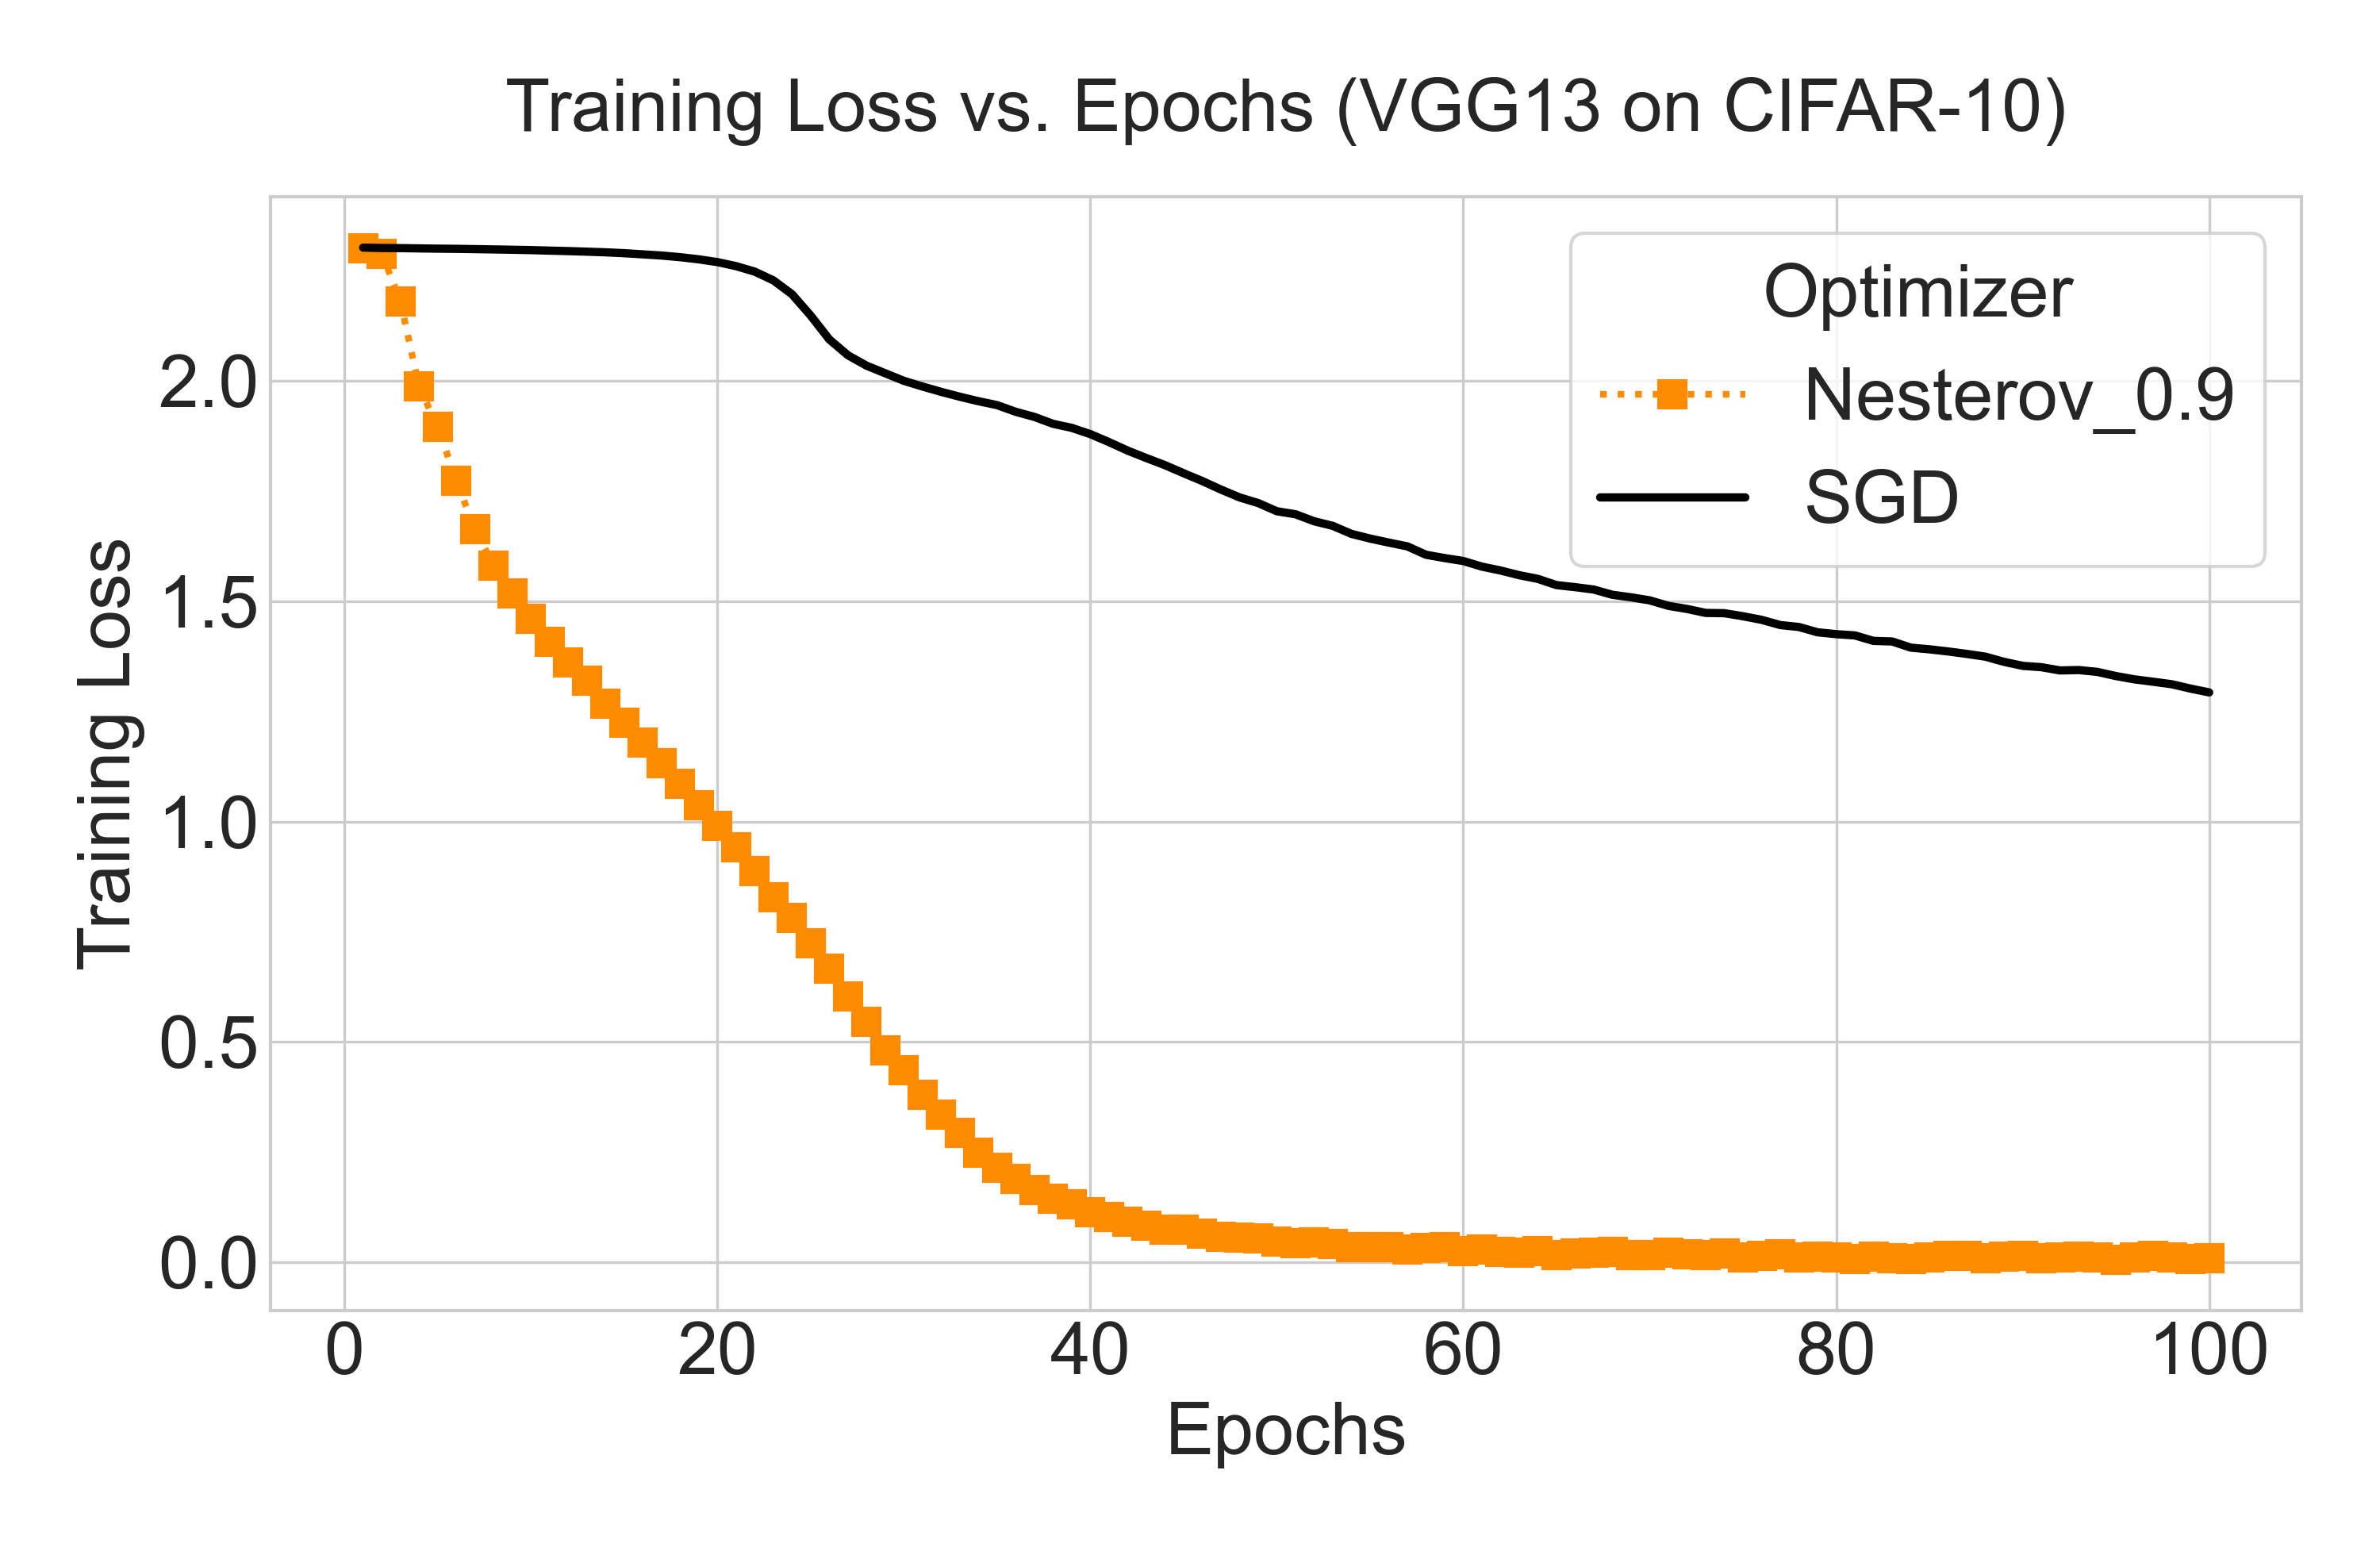
\includegraphics[width=0.48\textwidth]{Analysis_3_Impact_of_Momentum3_cifar_vgg13_training_loss.png}} \quad
    \subfloat[VGG13 Accuracy on CIFAR-10 ]{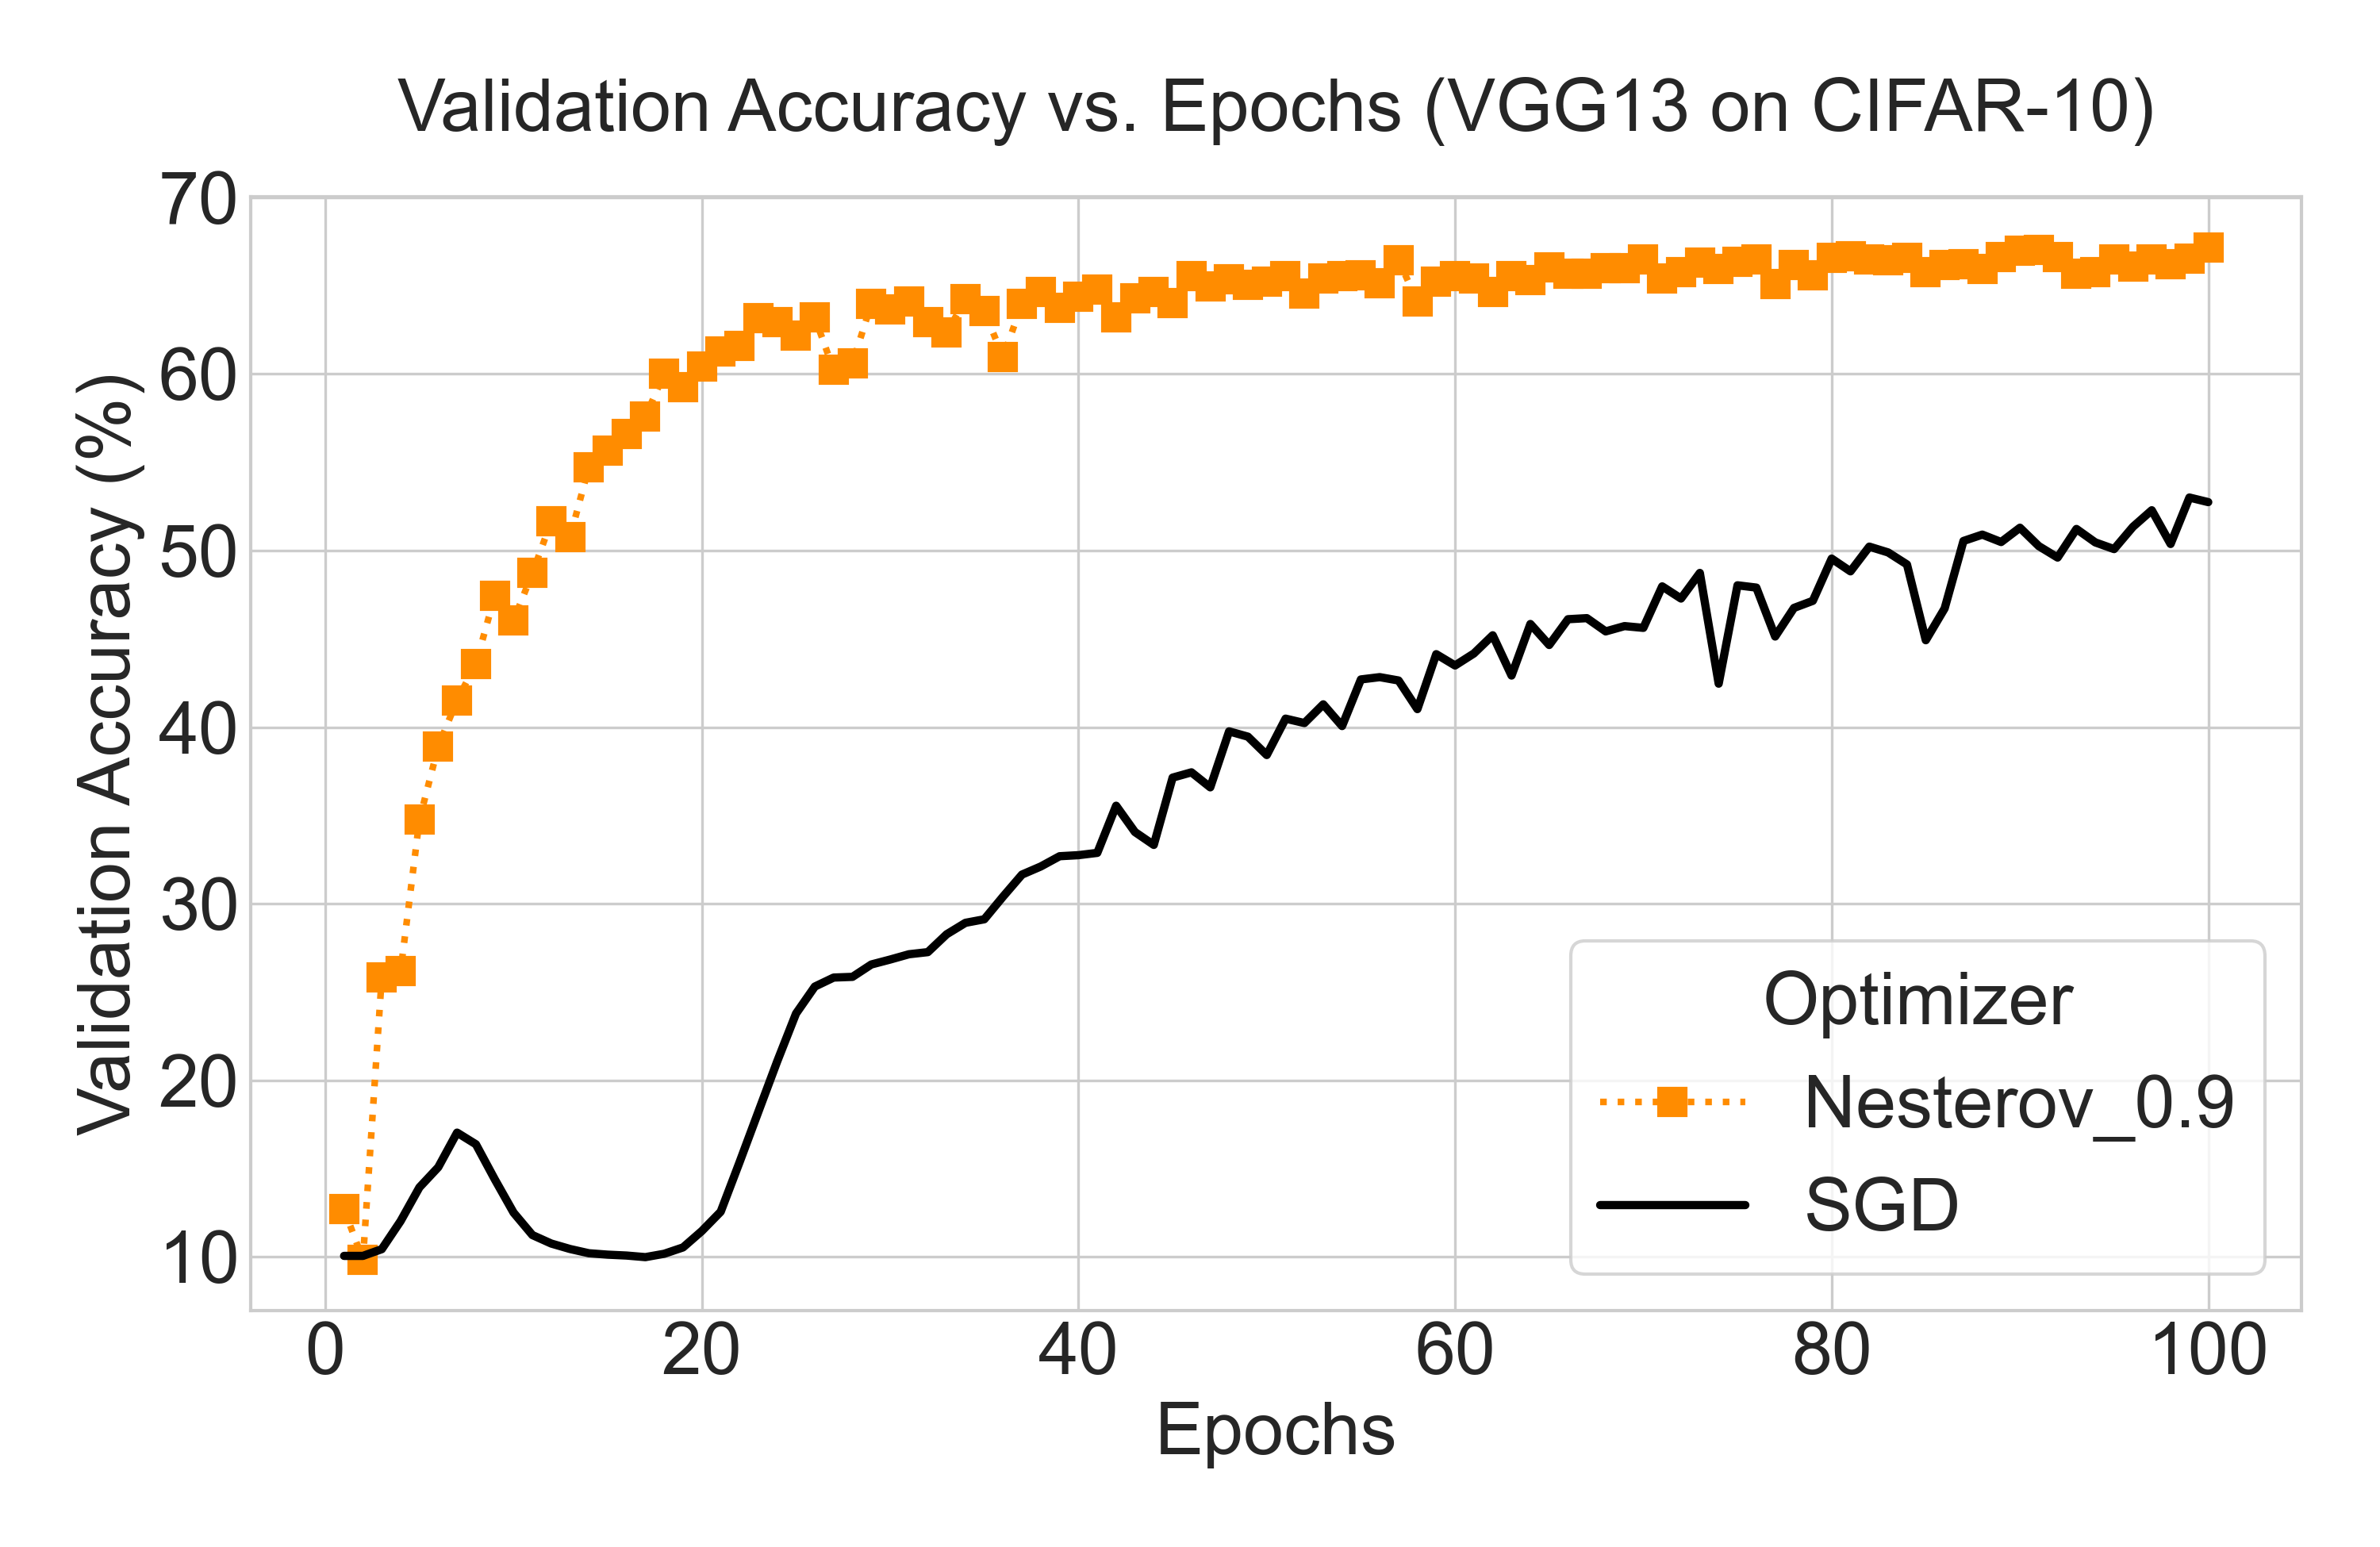
\includegraphics[width=0.48\textwidth]{Analysis_3_Impact_of_Momentum3_cifar_vgg13_validation_accuracy.png}}
    \caption{Impact of momentum: baseline method (SGD, black line) vs. baseline method with momentum (Nesterov, orange line)}
    \label{fig:momentum_study}
\end{figure}

Let's see the table:

\begin{table}[H]
\centering
\caption{Final Test Accuracy (Nesterov vs. SGD)}
\label{tab:nesterov_vs_sgd}
\begin{tabular}{|l|c|c|c|}
\hline
             & MLP on MNIST & CNN on CIFAR-10 & VGG13 on CIFAR-10 \\ \hline
Nesterov\_0.9 & \textbf{97.62\%} & \textbf{72.91\%}  & \textbf{66.02\%}    \\ \hline
SGD          & 91.82\%      & 50.64\%         & 52.68\%           \\ \hline
\end{tabular}
\end{table}


From the results of Experiment.3 and the final test accuracy, we can see that \textbf{the training performance with Nesterov momentum is significantly better than that of the baseline SGD.}

In the three training loss graphs, \textbf{Nesterov shows much steeper curves, indicating a faster convergence speed.}

In the three accuracy graphs, Nesterov also reaches a stable accuracy much more quickly, and the achieved accuracy is clearly higher than that of SGD.

We can also notice that in Figure 3.f, SGD experiences a sharp drop in accuracy between epochs 10–20, showing strong oscillations. This means \textbf{Nesterov is more stable than the baseline SGD.}

From a theoretical perspective, Nesterov momentum updates parameters by considering a predicted future position, allowing it to anticipate the upcoming gradient direction and make a better update. In contrast, standard SGD moves purely based on inertia without considering future gradients, which can cause it to oscillate repeatedly in regions with high curvature and become less stable.

In terms of final generalization performance, Nesterov clearly outperforms SGD. On the CNN task with CIFAR-10, Nesterov achieves almost 50 percent higher accuracy compared to SGD, demonstrating that \textbf{Nesterov has a much better accuracy and perform much better on generalization.}


%--------------------------------------------
\subsection{Joint Impact of Exponential Moving Average and Momentum (Adam)}

\begin{figure}[htbp]
    \centering
    % MLP row
    \subfloat[MLP Loss on MNIST]{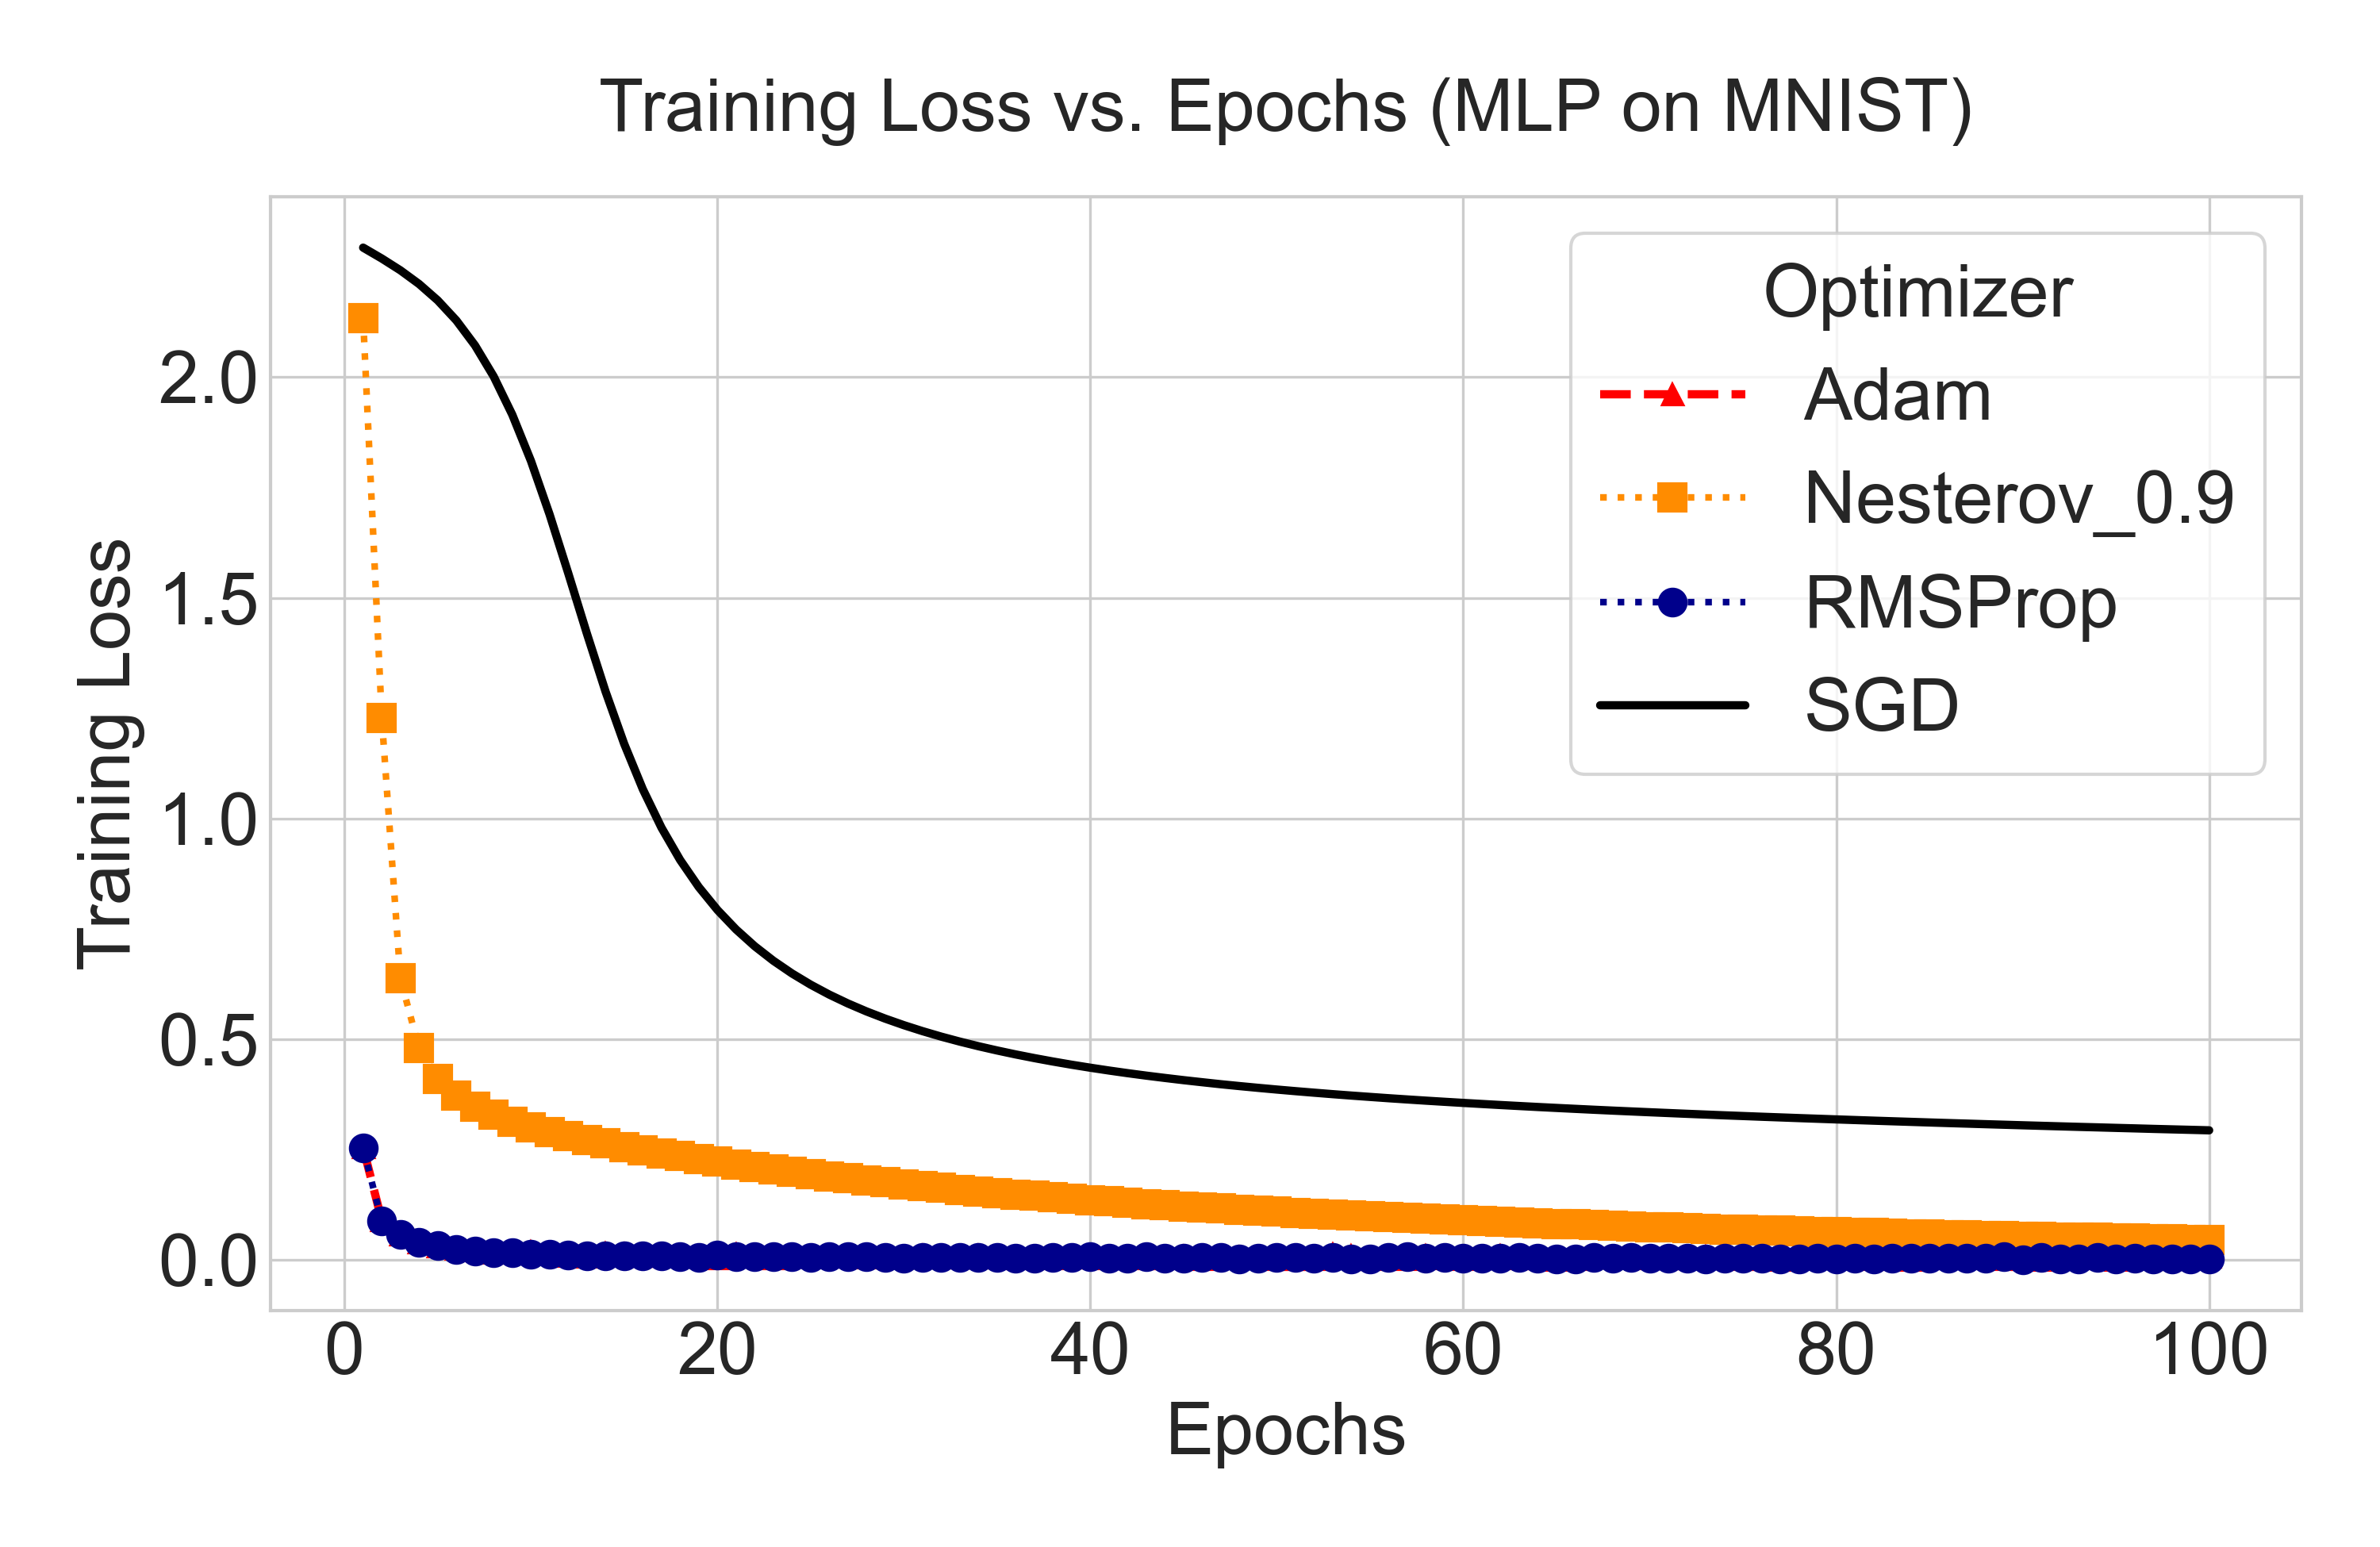
\includegraphics[width=0.48\textwidth]{Analysis_4_Joint_Impact1_mnist_mlp_training_loss.png}} \quad
    \subfloat[MLP Accuracy on MNIST]{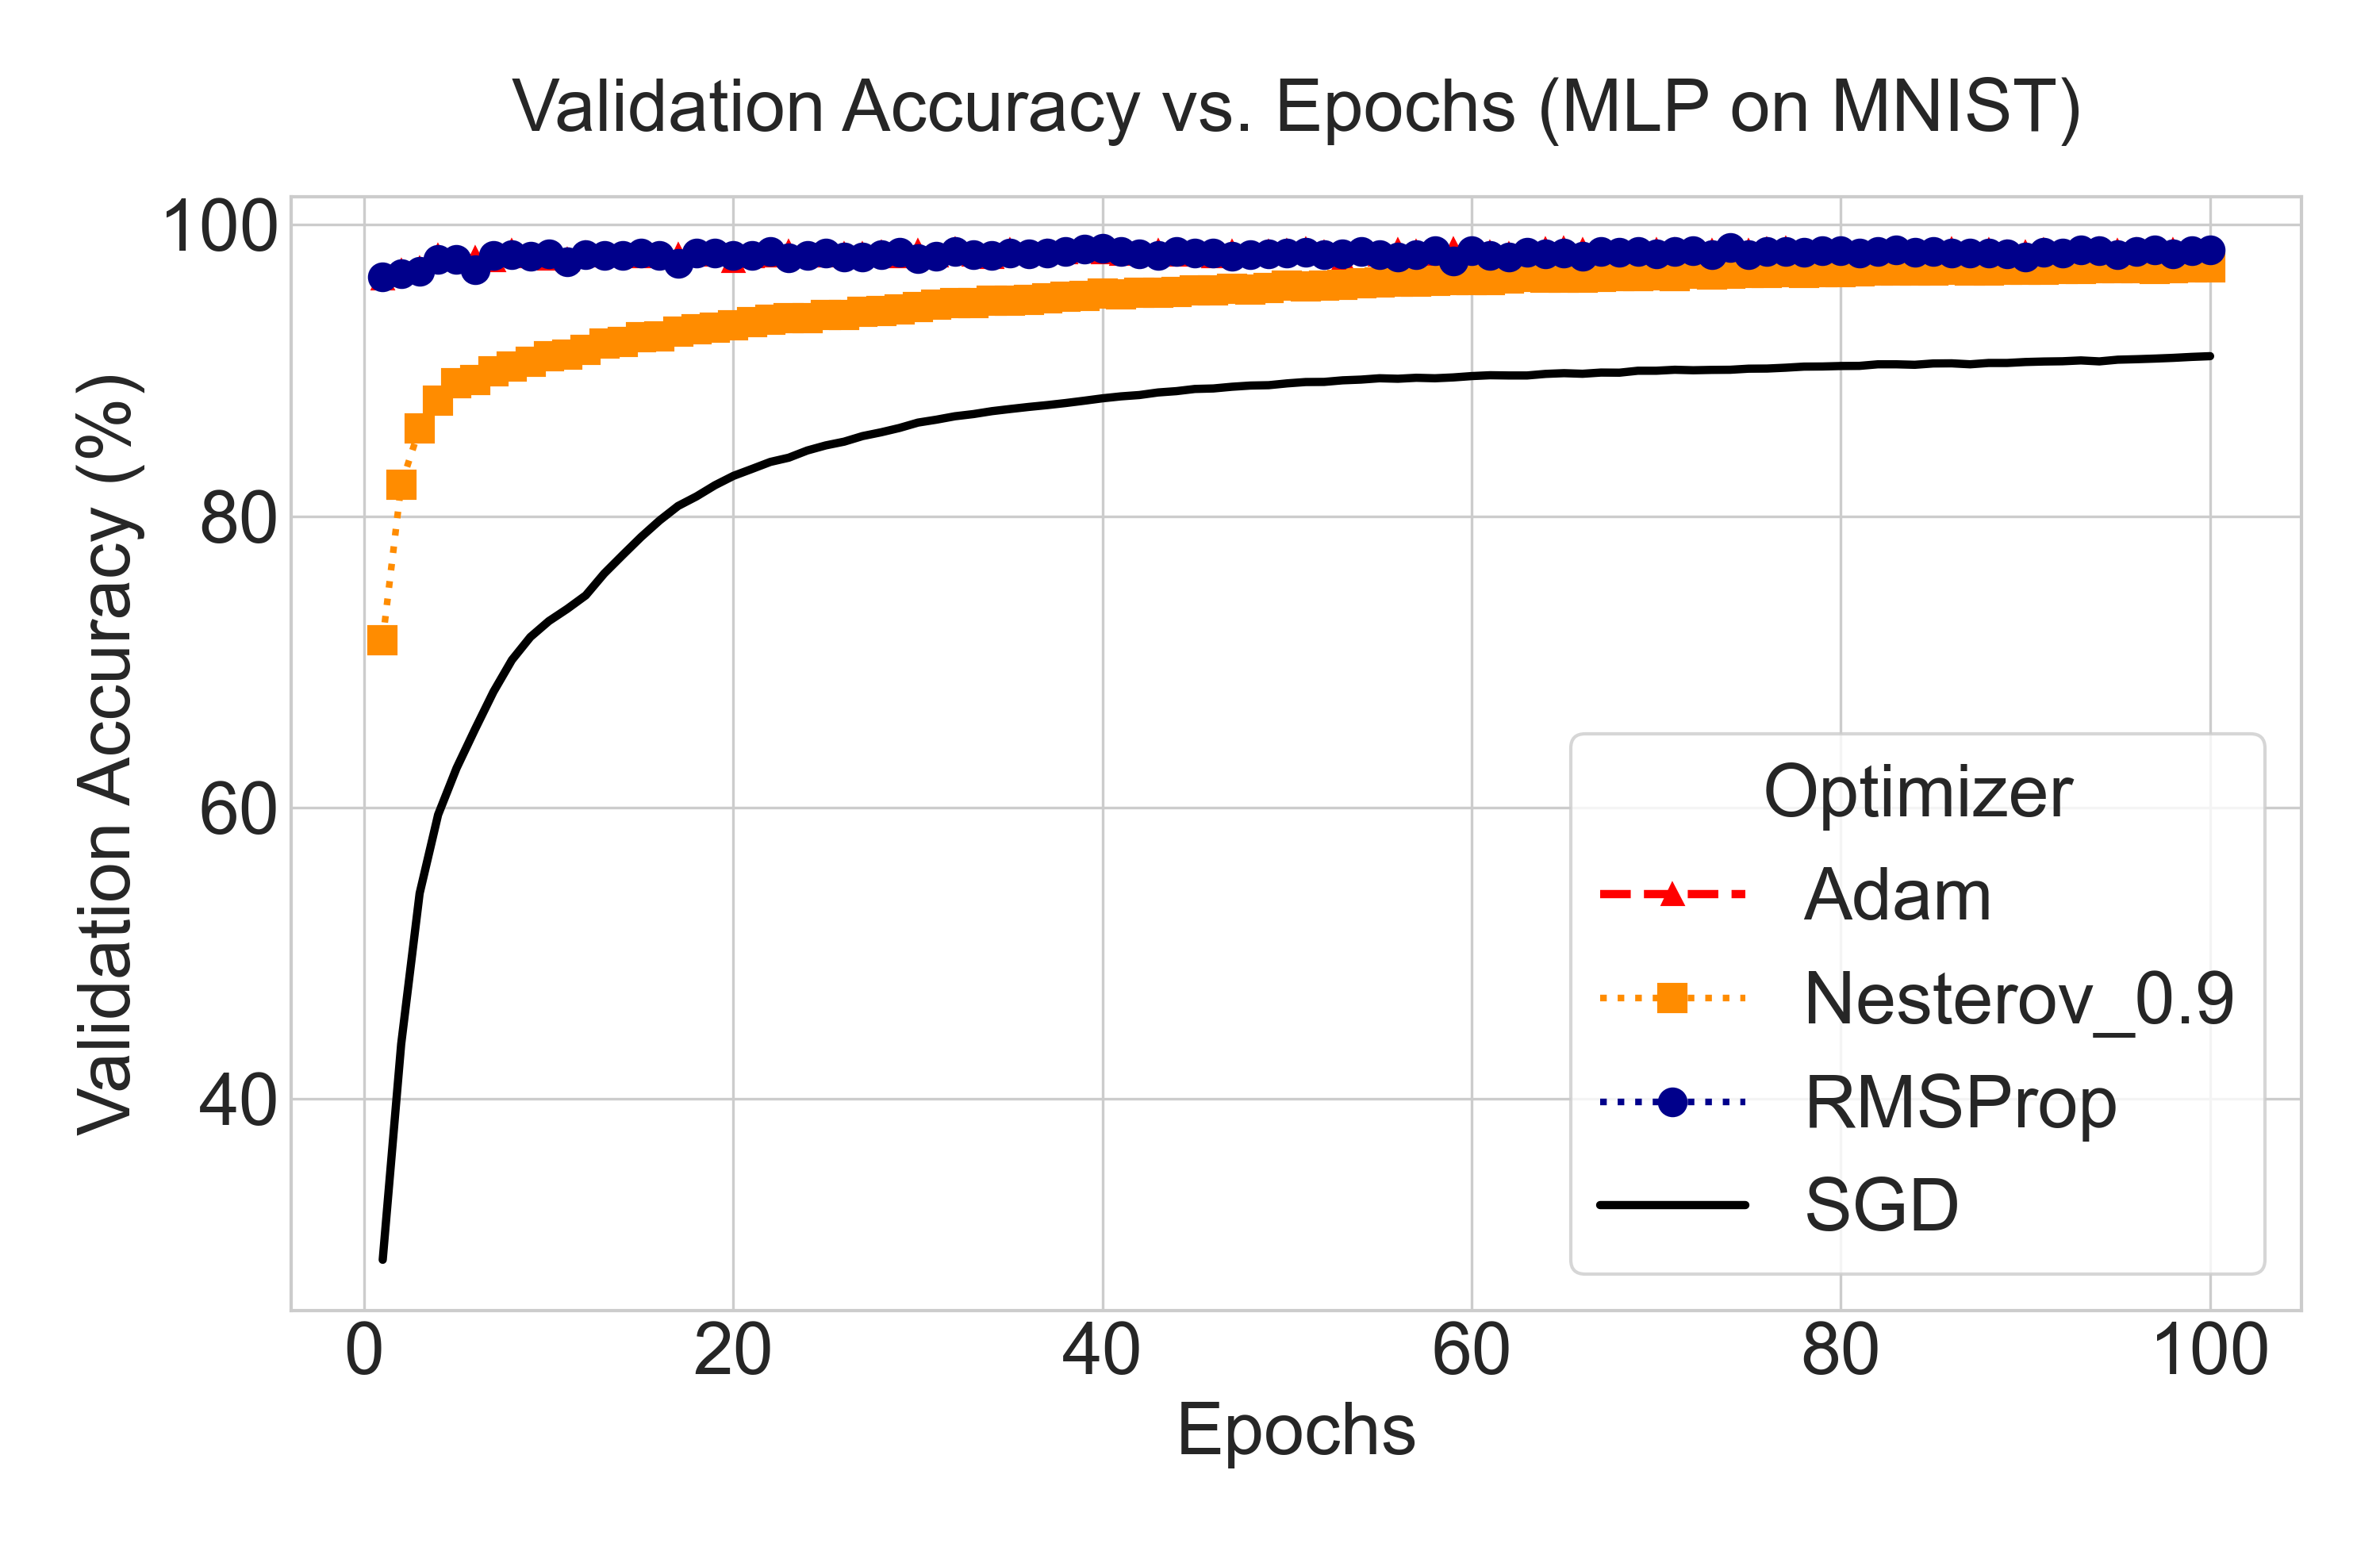
\includegraphics[width=0.48\textwidth]{Analysis_4_Joint_Impact1_mnist_mlp_validation_accuracy.png}} \\
    % CNN row
    \subfloat[CNN Loss on CIFAR-10]{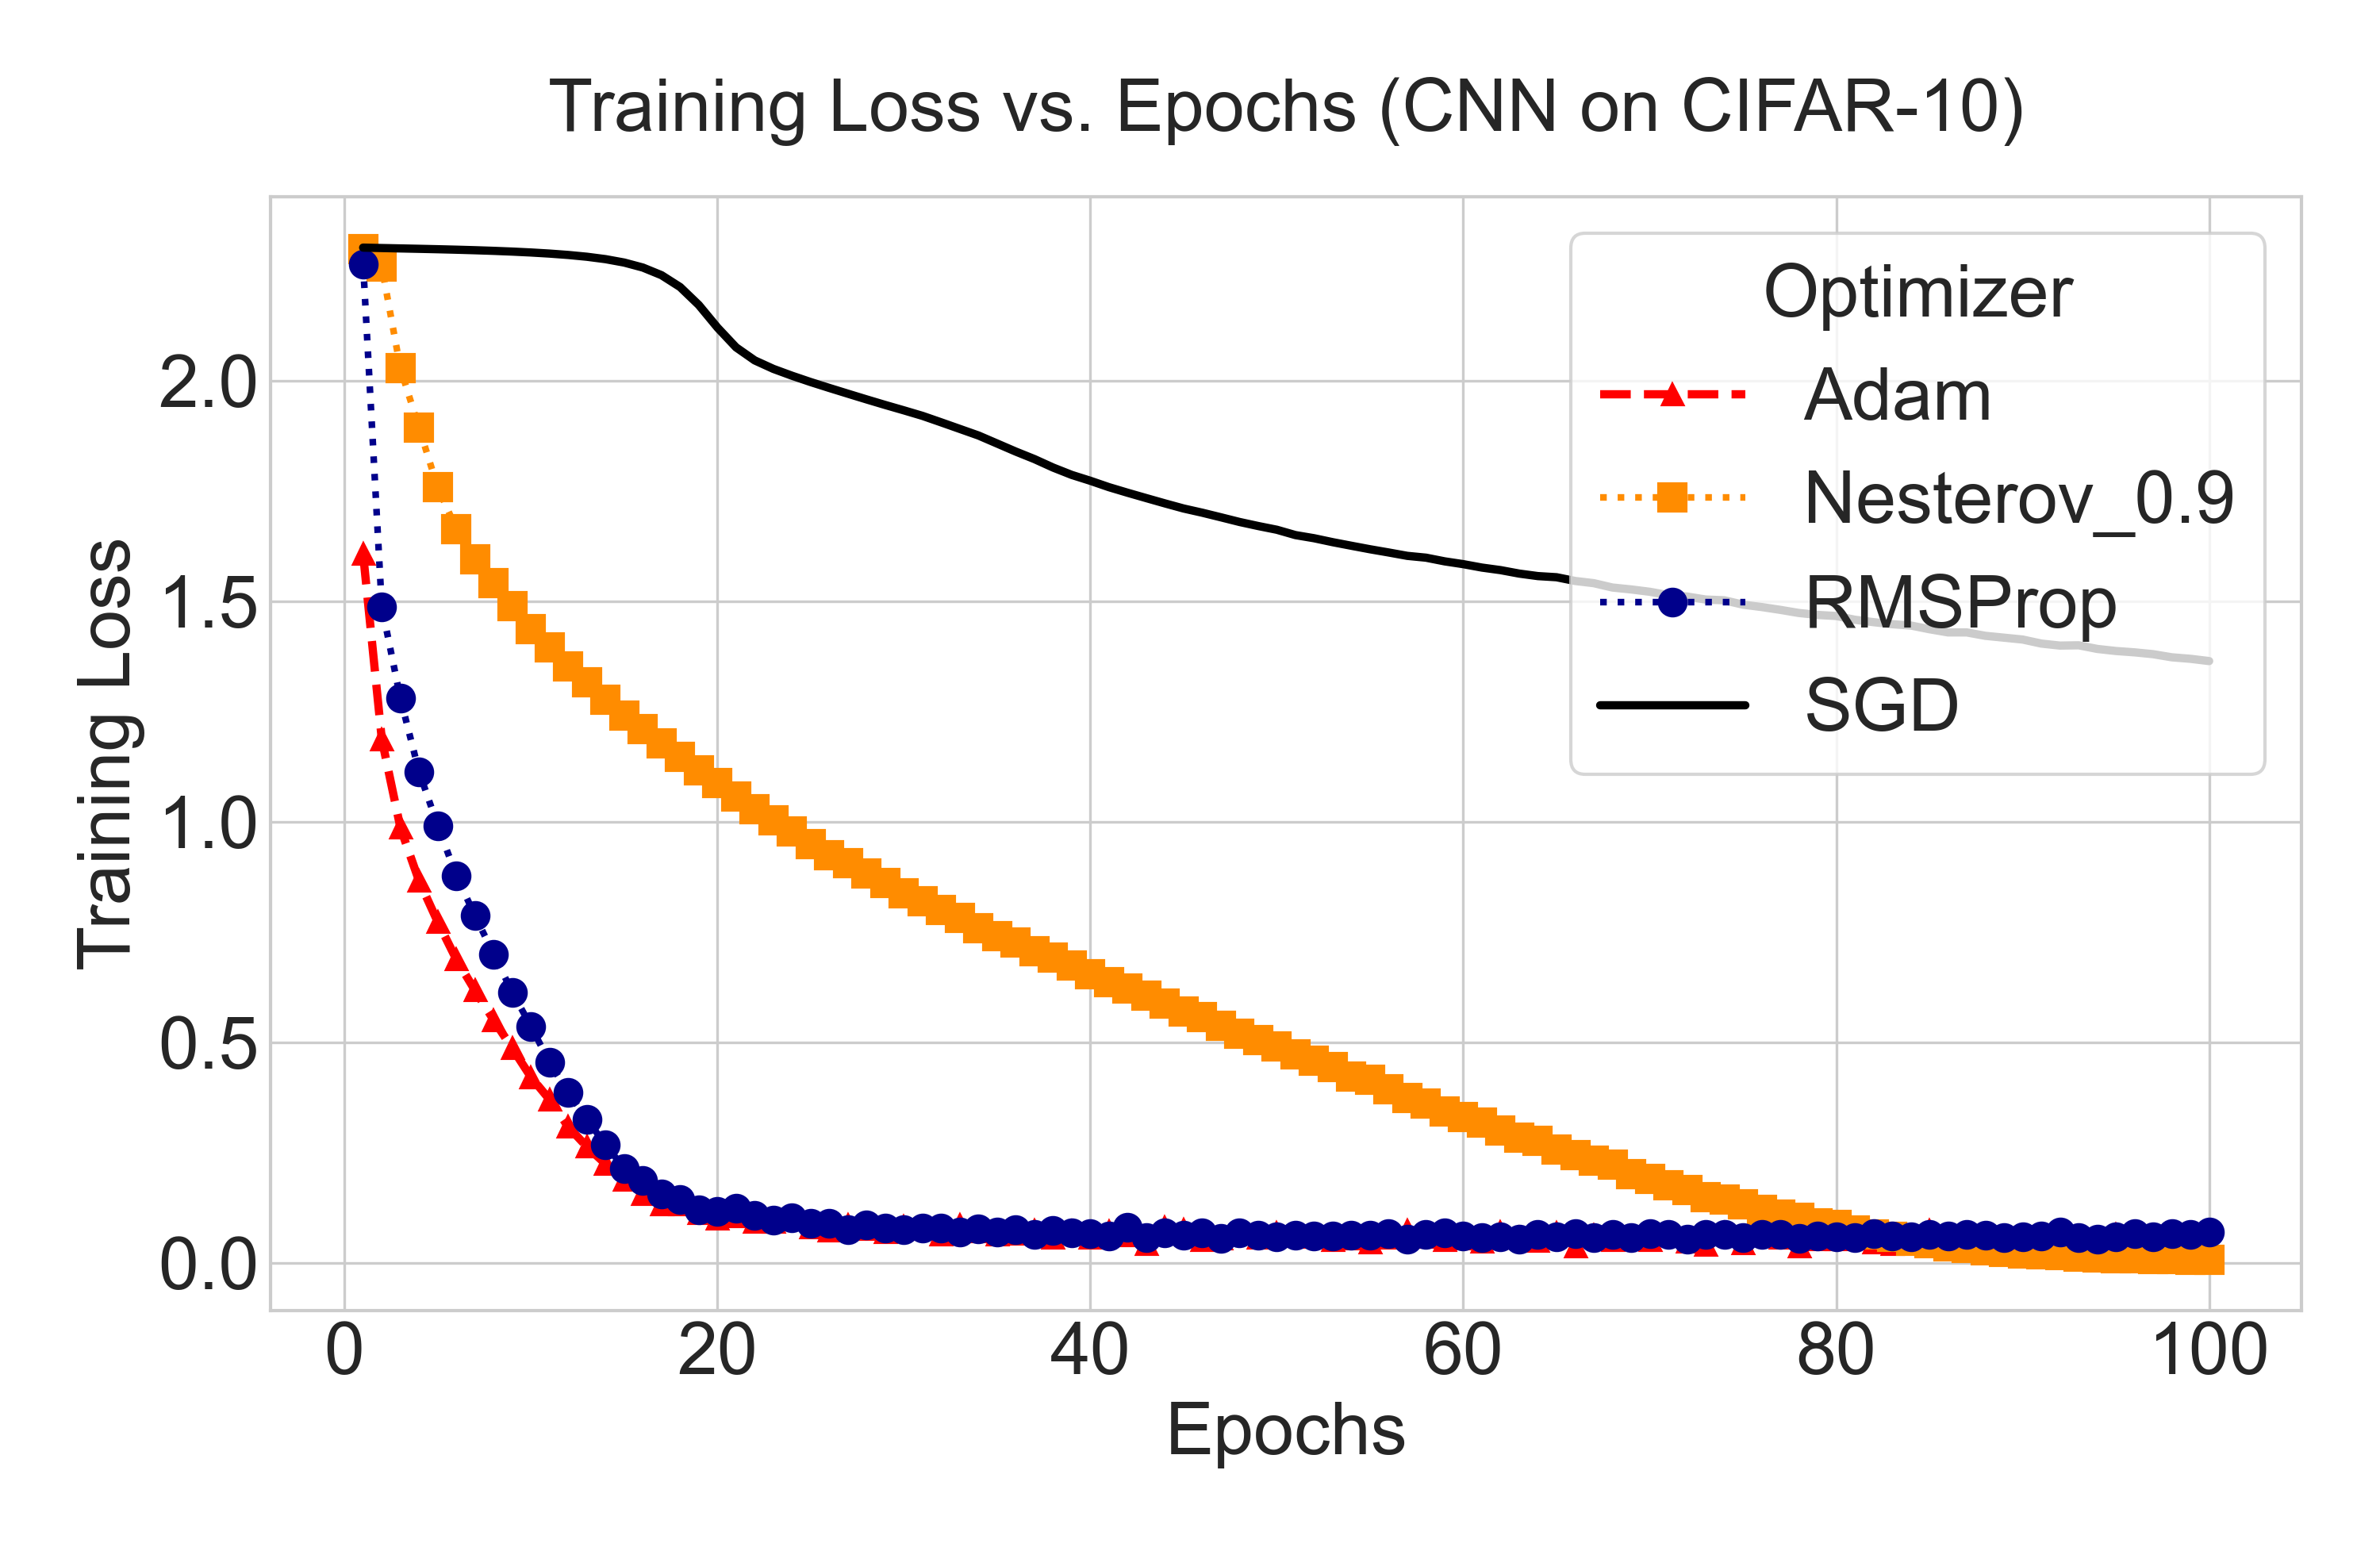
\includegraphics[width=0.48\textwidth]{Analysis_4_Joint_Impact2_cifar10_cnn_training_loss.png}} \quad
    \subfloat[CNN Accuracy on CIFAR-10]{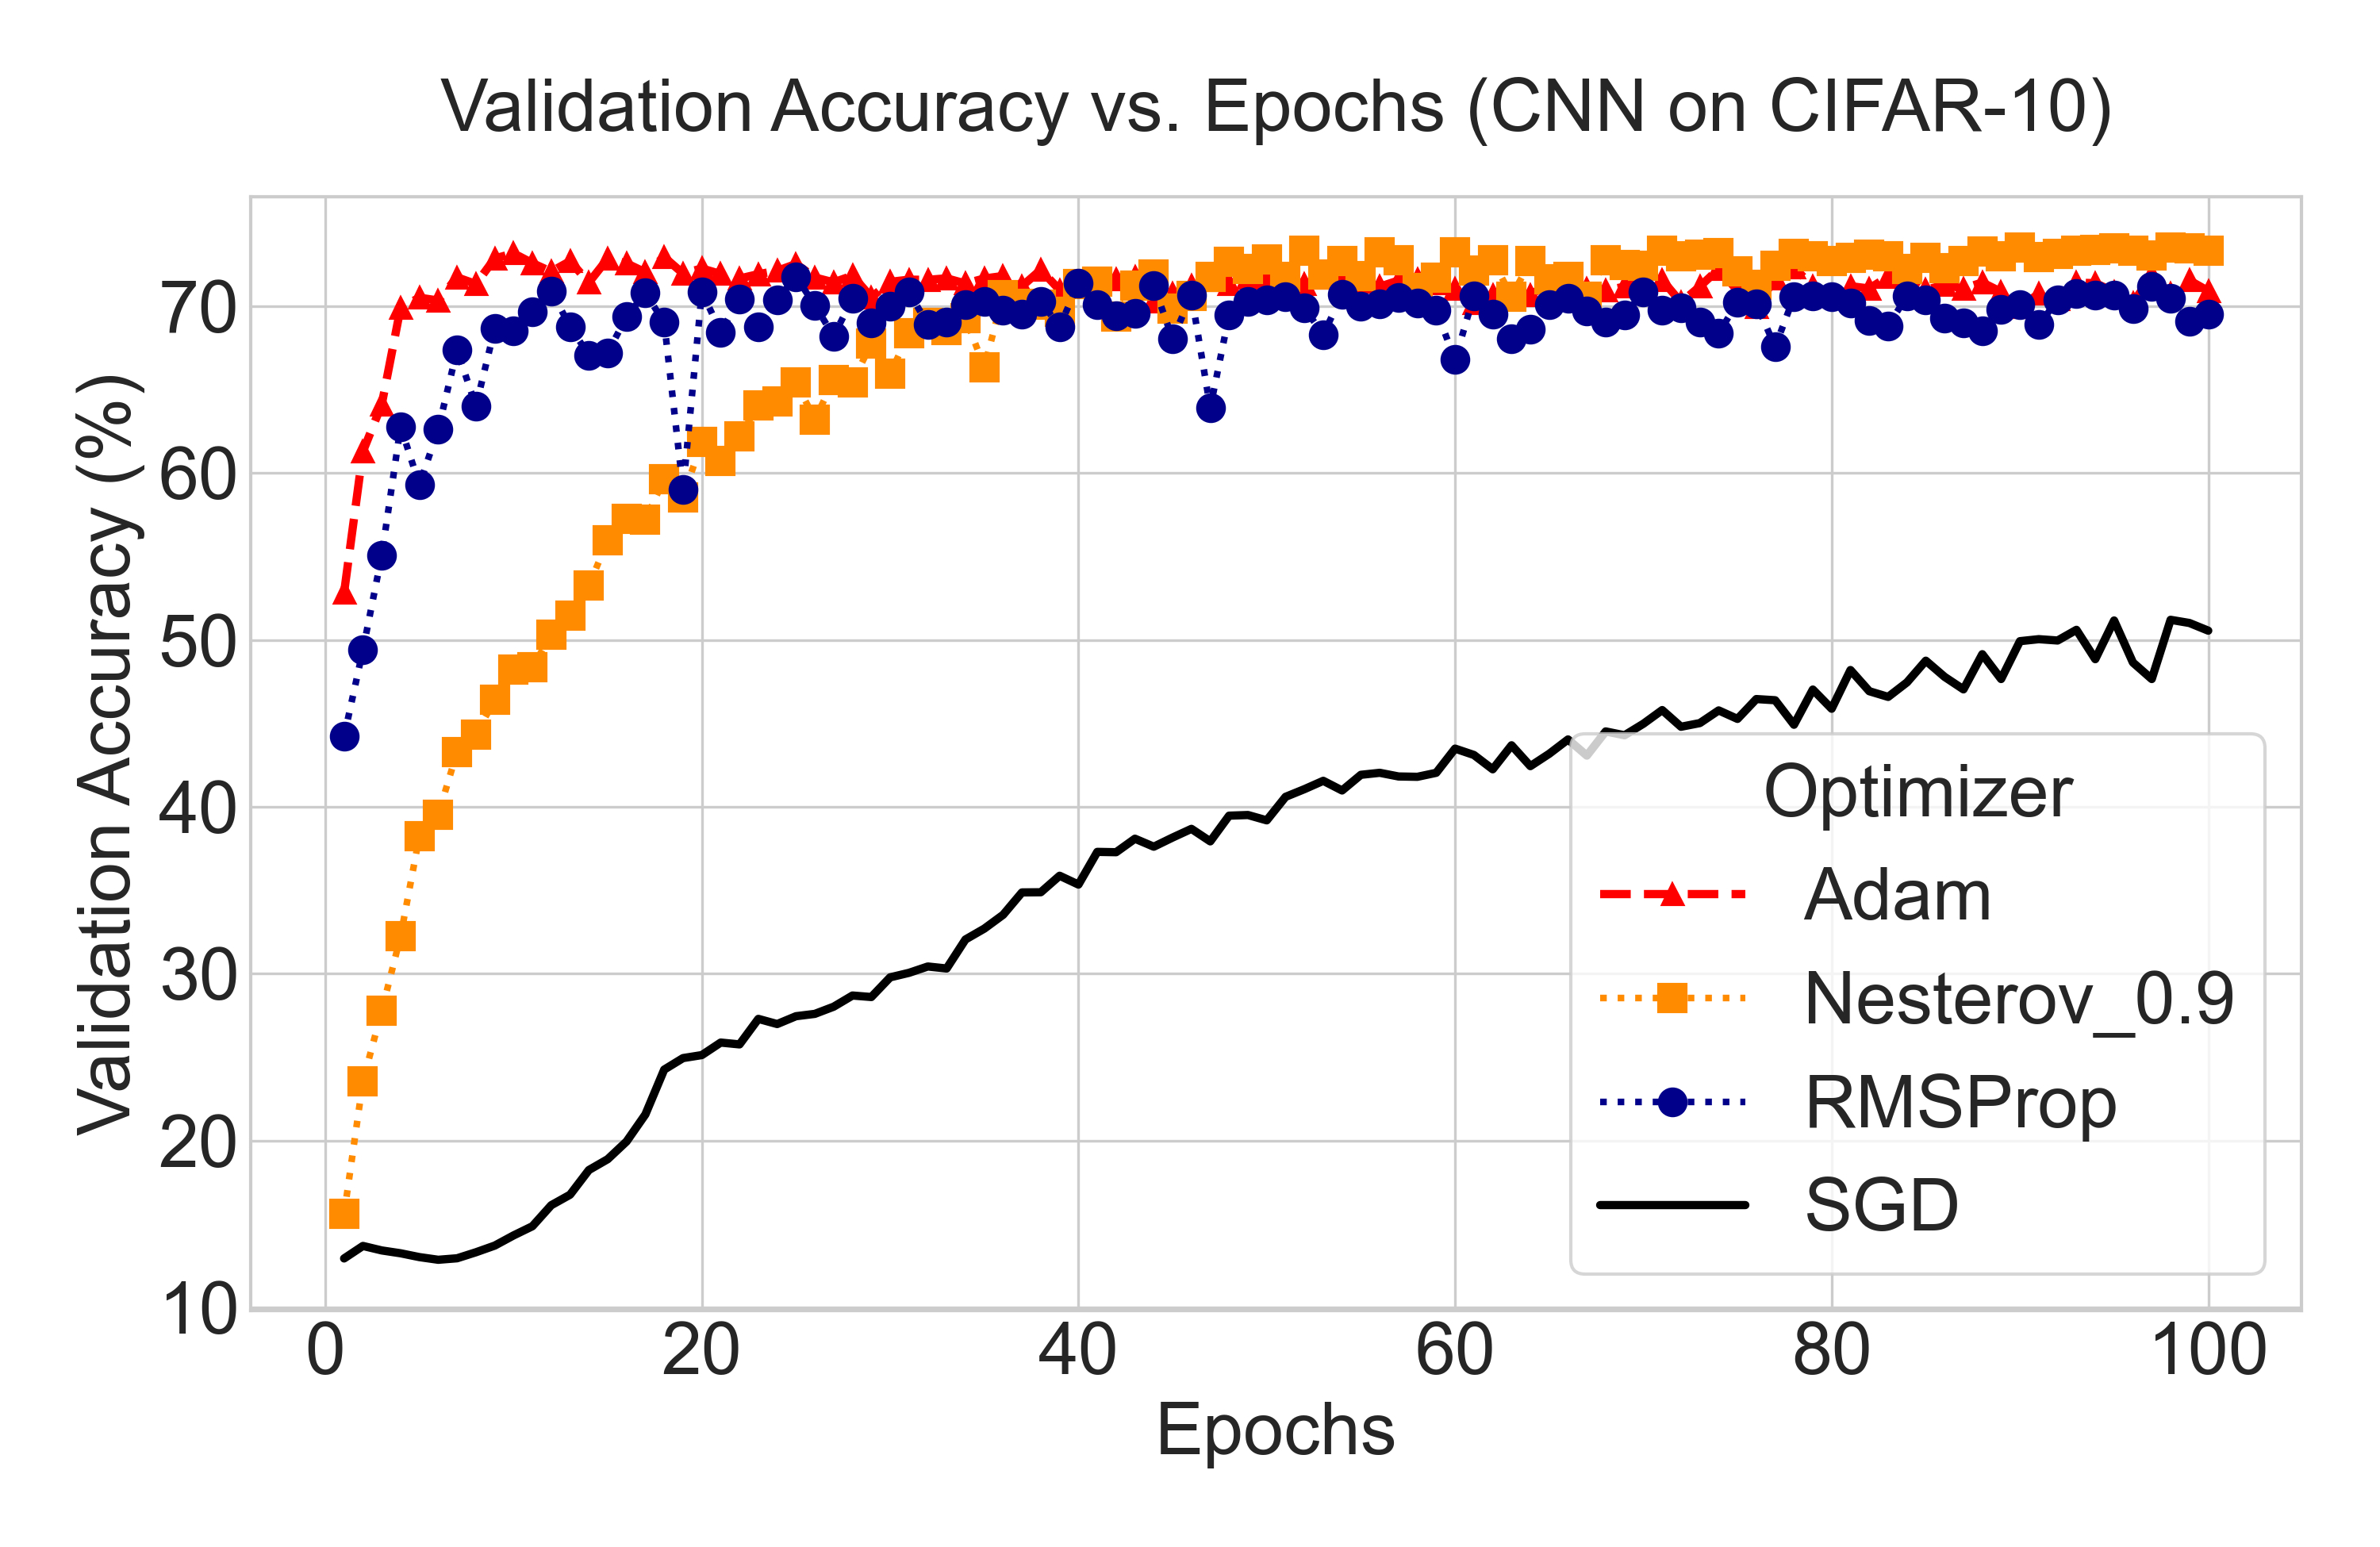
\includegraphics[width=0.48\textwidth]{Analysis_4_Joint_Impact2_cifar10_cnn_validation_accuracy.png}} \\
    % VGG13 row
    \subfloat[VGG13 Loss on CIFAR-10]{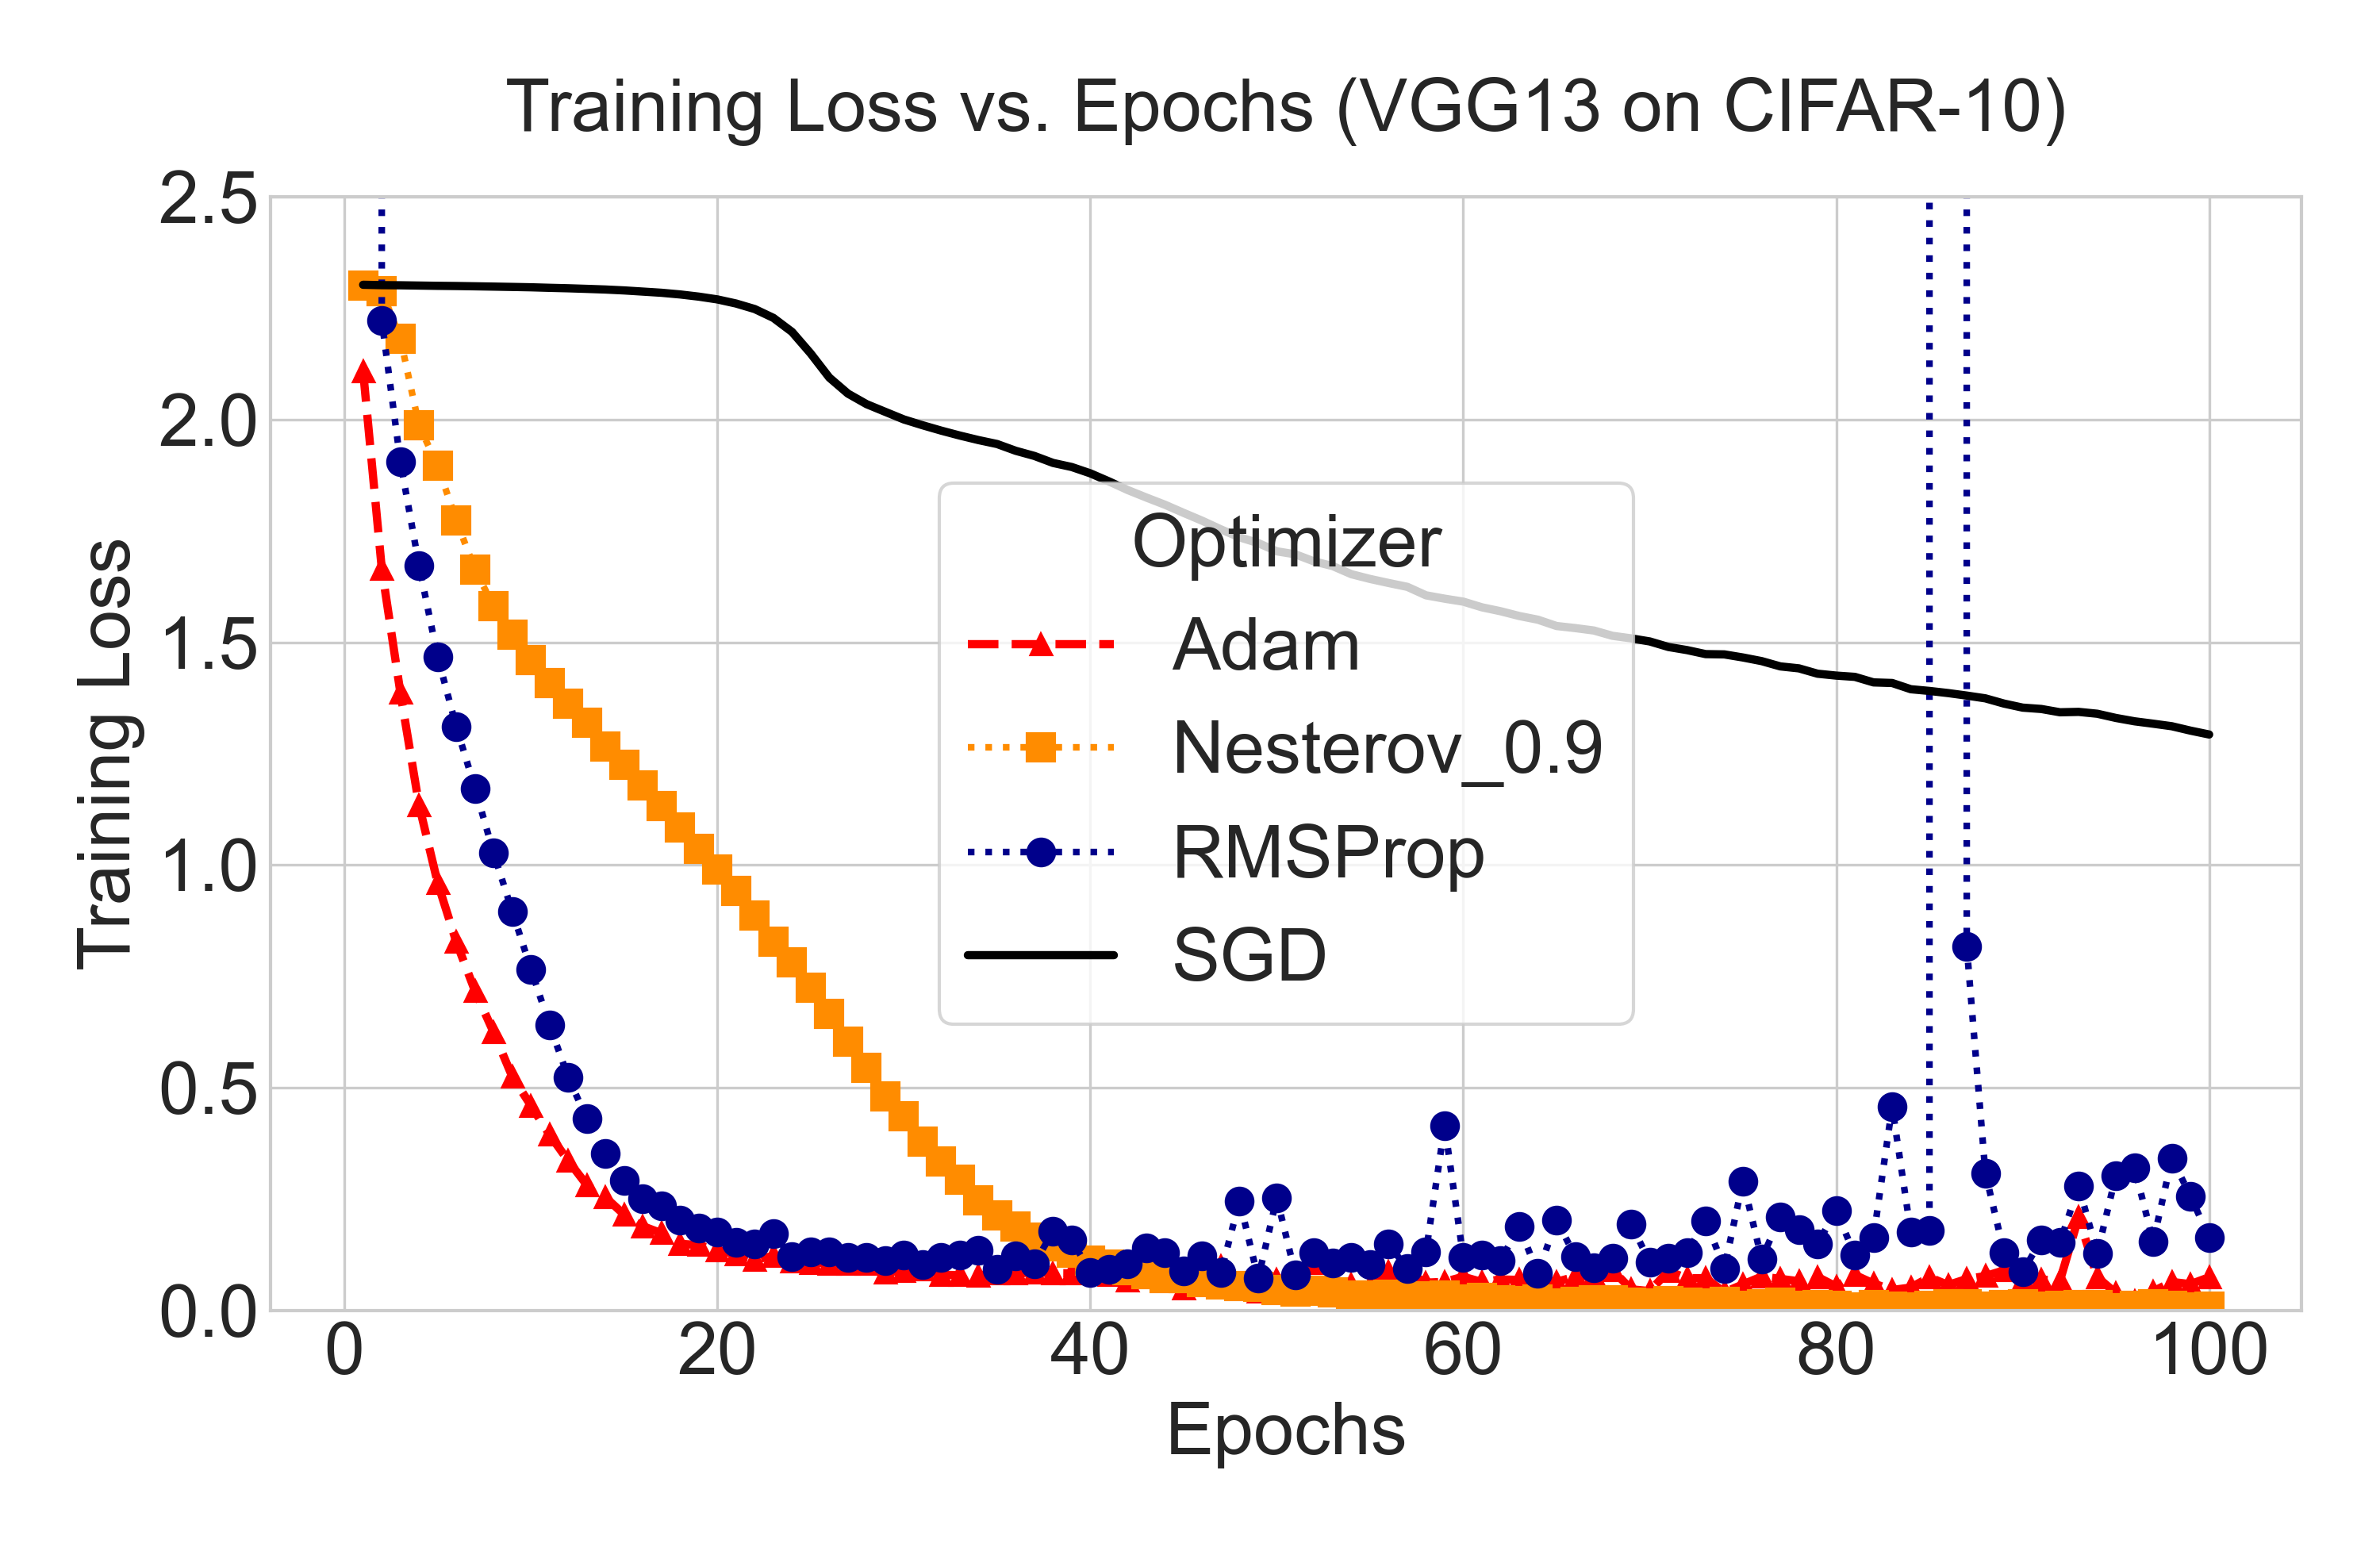
\includegraphics[width=0.48\textwidth]{Analysis_4_Joint_Impact3_cifar_vgg13_training_loss.png}} \quad
    \subfloat[VGG13 Accuracy on CIFAR-10]{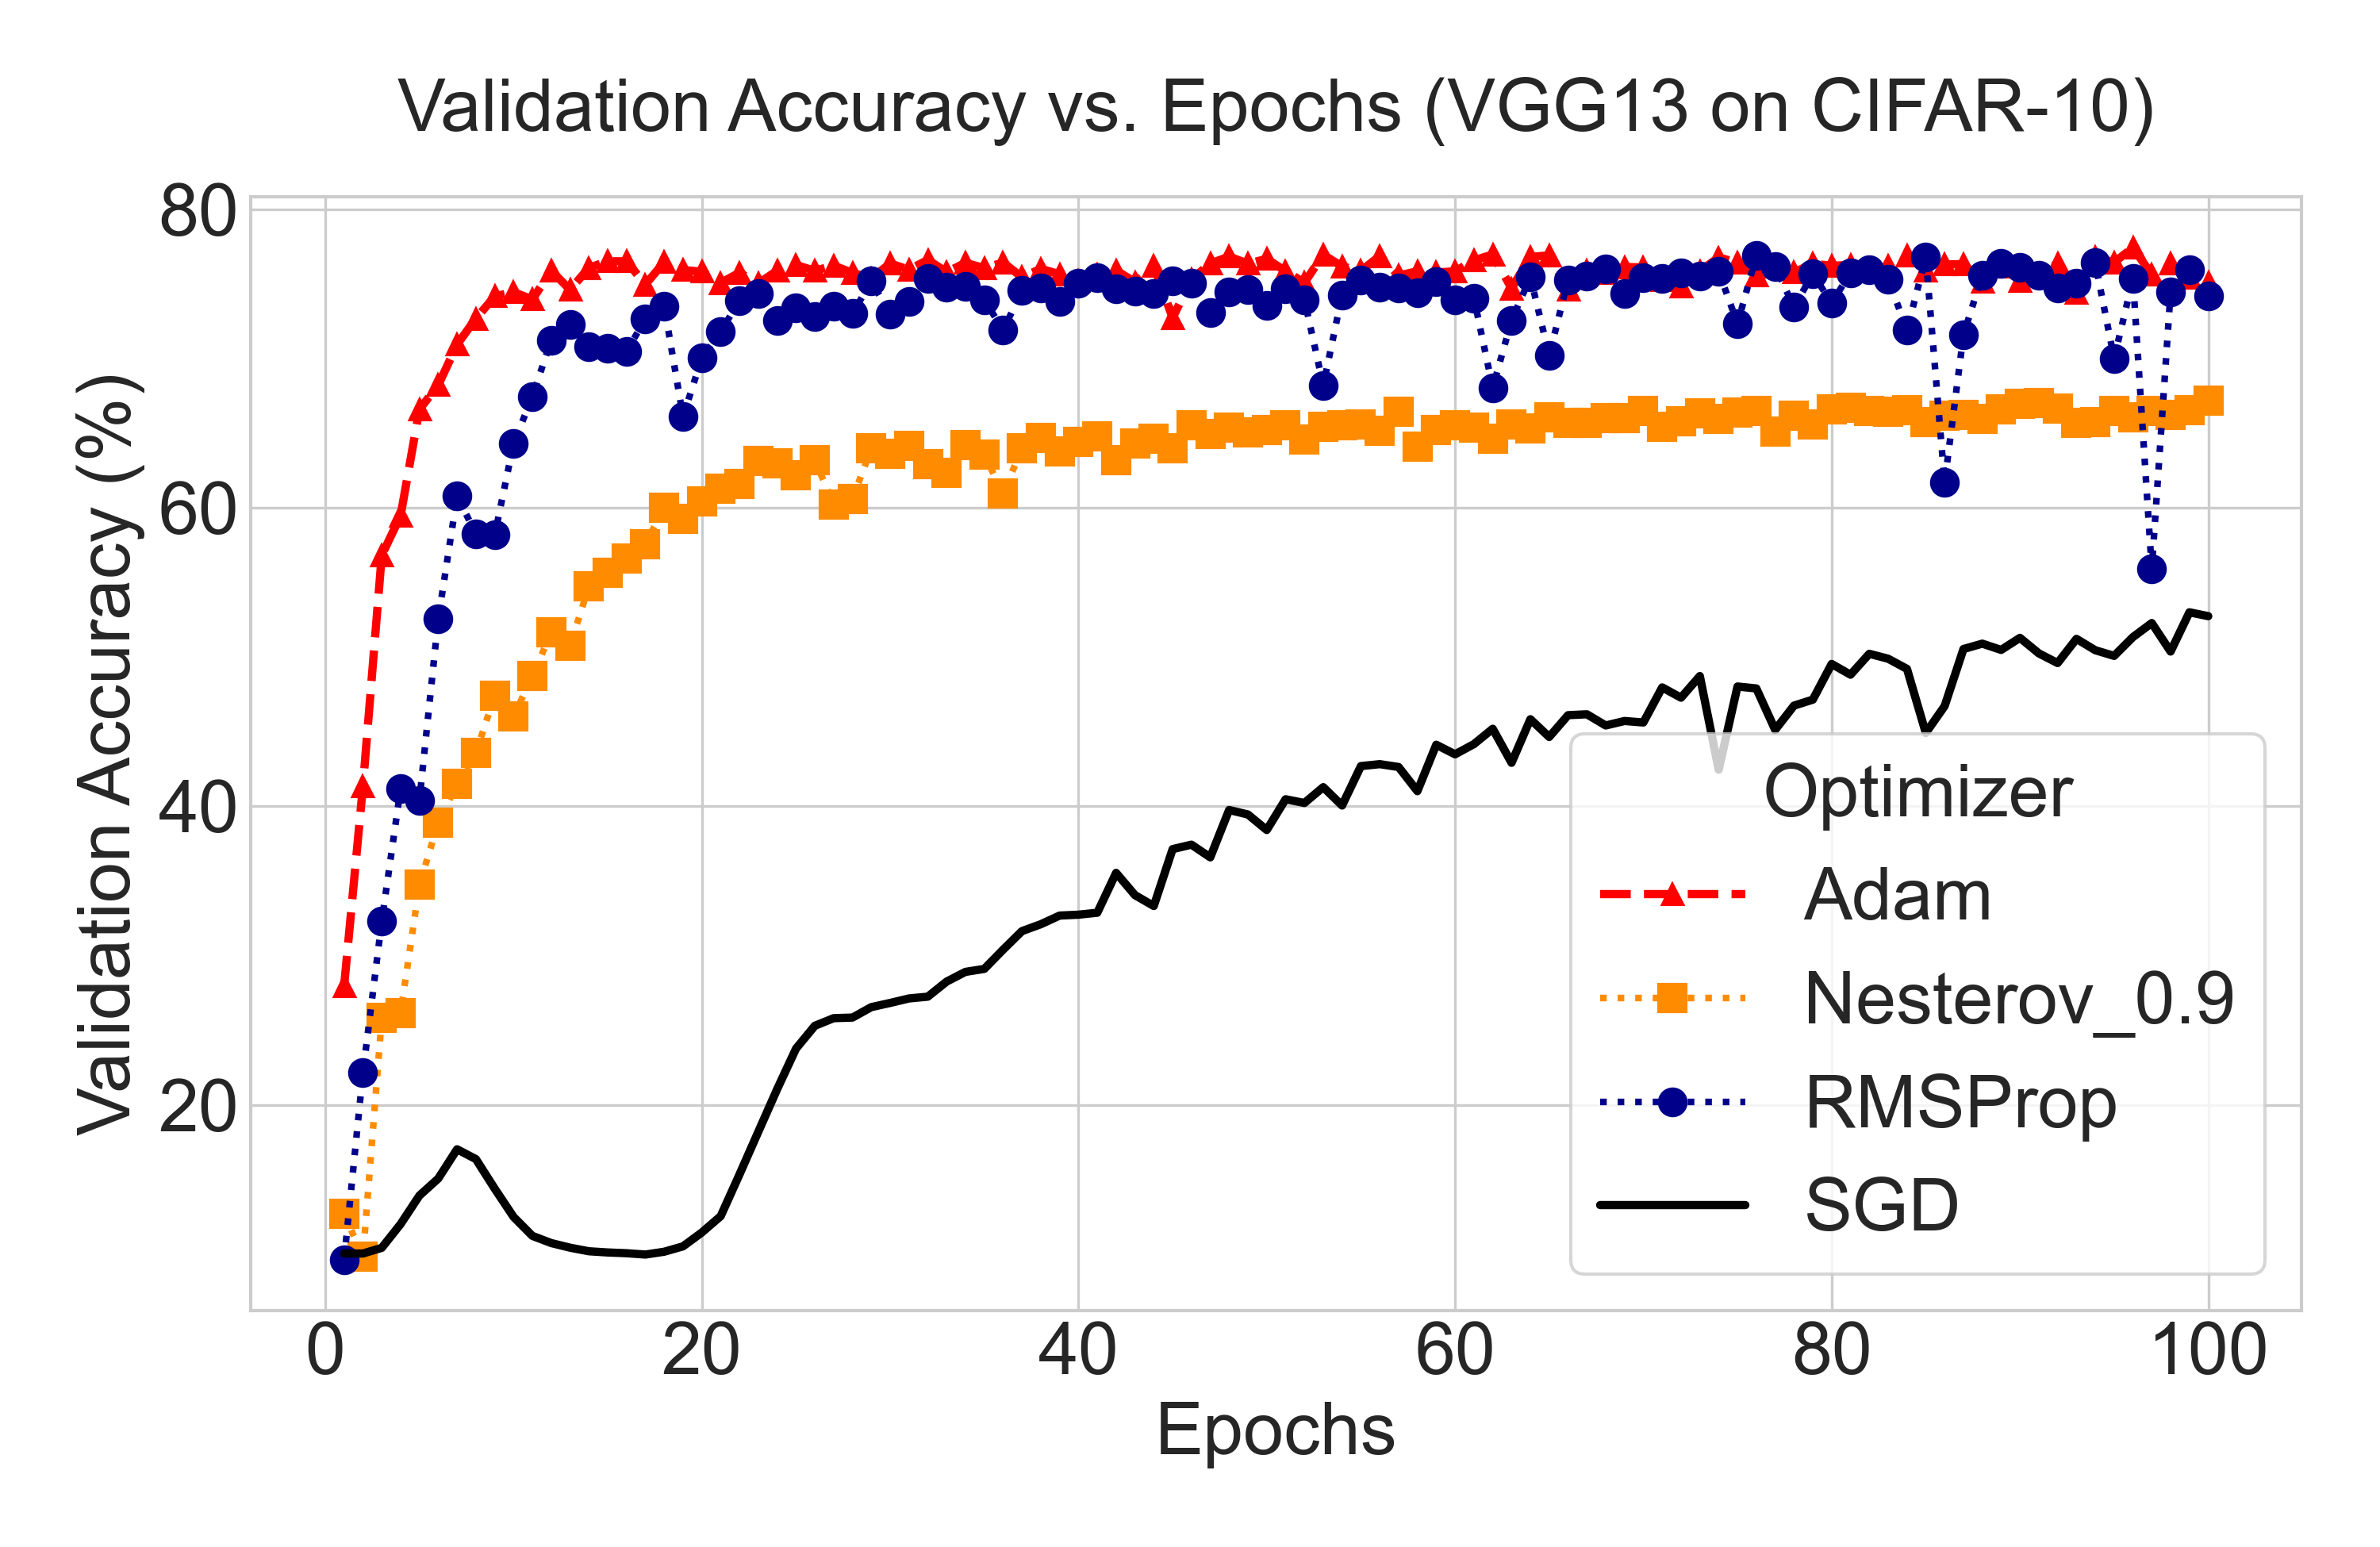
\includegraphics[width=0.48\textwidth]{Analysis_4_Joint_Impact3_cifar_vgg13_validation_accuracy.png}}
    \caption{Joint impact of exponential moving average and momentum: baseline methods (SGD, Nesterov, RMSProp) vs. method with joint impact (Adam, red line)}
    \label{fig:joint_impact_study}
\end{figure}

\begin{table}[H]
\centering
\caption{Final Test Accuracy (Joint Impact)}
\label{tab:joint_impact}
\begin{tabular}{|l|c|c|c|}
\hline
             & MLP on MNIST & CNN on CIFAR-10 & VGG13 on CIFAR-10 \\ \hline
Adam         & \textbf{98.32\%} & 70.15\%         & \textbf{74.61\%}    \\ \hline
RMSProp      & 98.29\%      & 68.65\%         & 73.61\%           \\ \hline
Nesterov\_0.9 & 97.62\%      & \textbf{72.91\%}  & 66.02\%           \\ \hline
SGD          & 91.82\%      & 50.64\%         & 52.68\%           \\ \hline
\end{tabular}
\end{table}

In Experiment 4, we compared RMSProp (which performed better in Experiment 2), Nesterov (which performed better in Experiment 3), and Adam (which combines the advantages of both).

\subsubsection{MLP on MNIST}

From the training loss and validation accuracy, we find the following:
In Figures a and b, Adam and RMSProp perform best but are highly overlapping. We compare their detailed plots for epochs 80-100:


\begin{figure}[H]
    \centering
    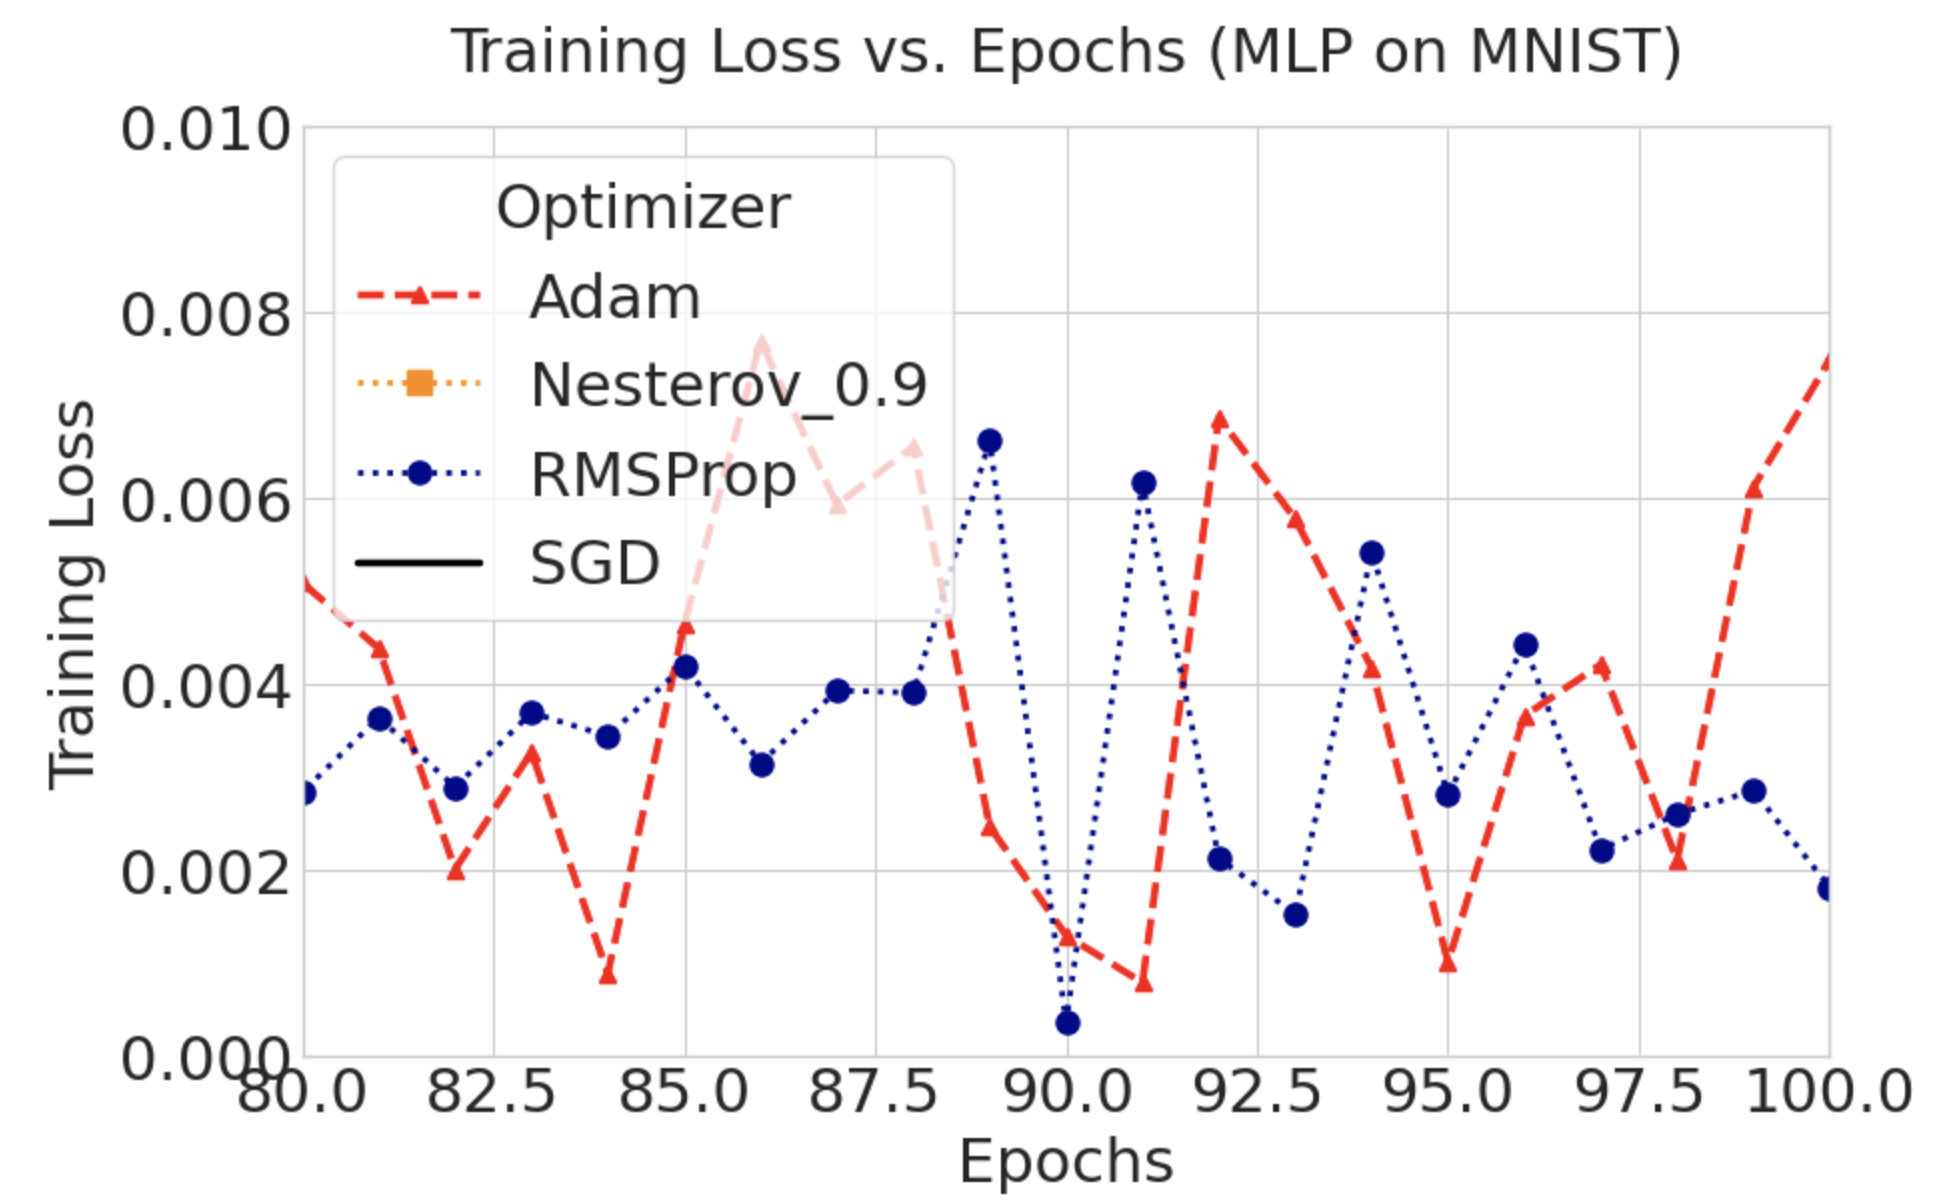
\includegraphics[width=0.45\textwidth]{1-1.png}
    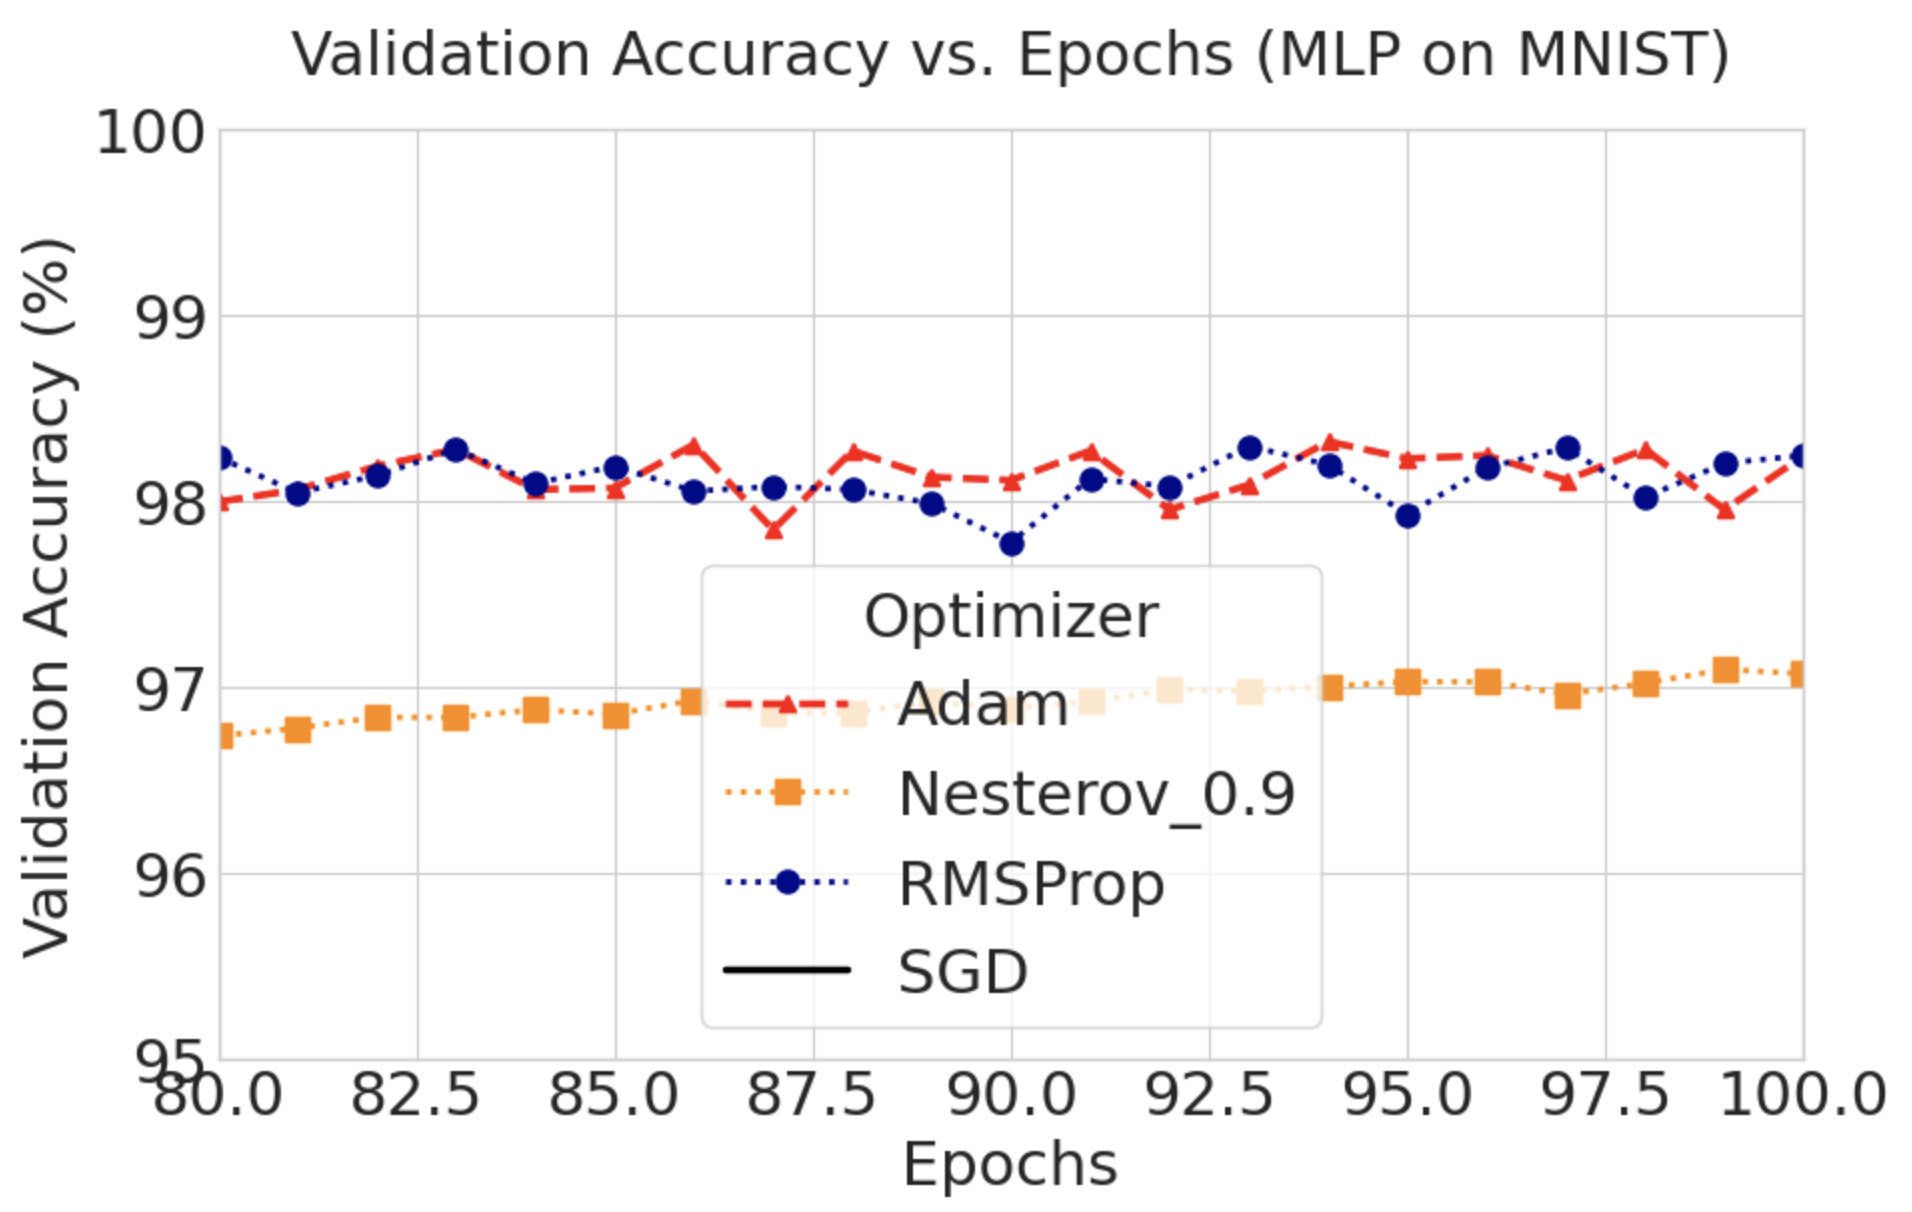
\includegraphics[width=0.45\textwidth]{1-2.png}
    \caption{Detailed plots for epochs 80-100, MLP on MNIST}
    \label{fig:detailed_mlp_on_mnist}
\end{figure}

From the figure above, we can find that during training epochs 80-100, the training loss of Adam and RMSProp fluctuated around the same level; their validation accuracy also fluctuated around the same level. We can also see that their performance on the final test set was very similar, \textbf{so on the MLP on MNIST task, Adam and RMSProp can be considered equally good. They both outperform Nesterov: Adam and RMSProp converge faster, have higher accuracy, and achieve better final test set accuracy and generalization capabilities.}


\subsubsection{CNN on CIFAR-10}

In Figures c and d, although Adam and RMSProp converge faster, Nesterov ultimately achieves superior performance. We compare their detailed plots for epochs 80-100:

\begin{figure}[H]
    \centering
    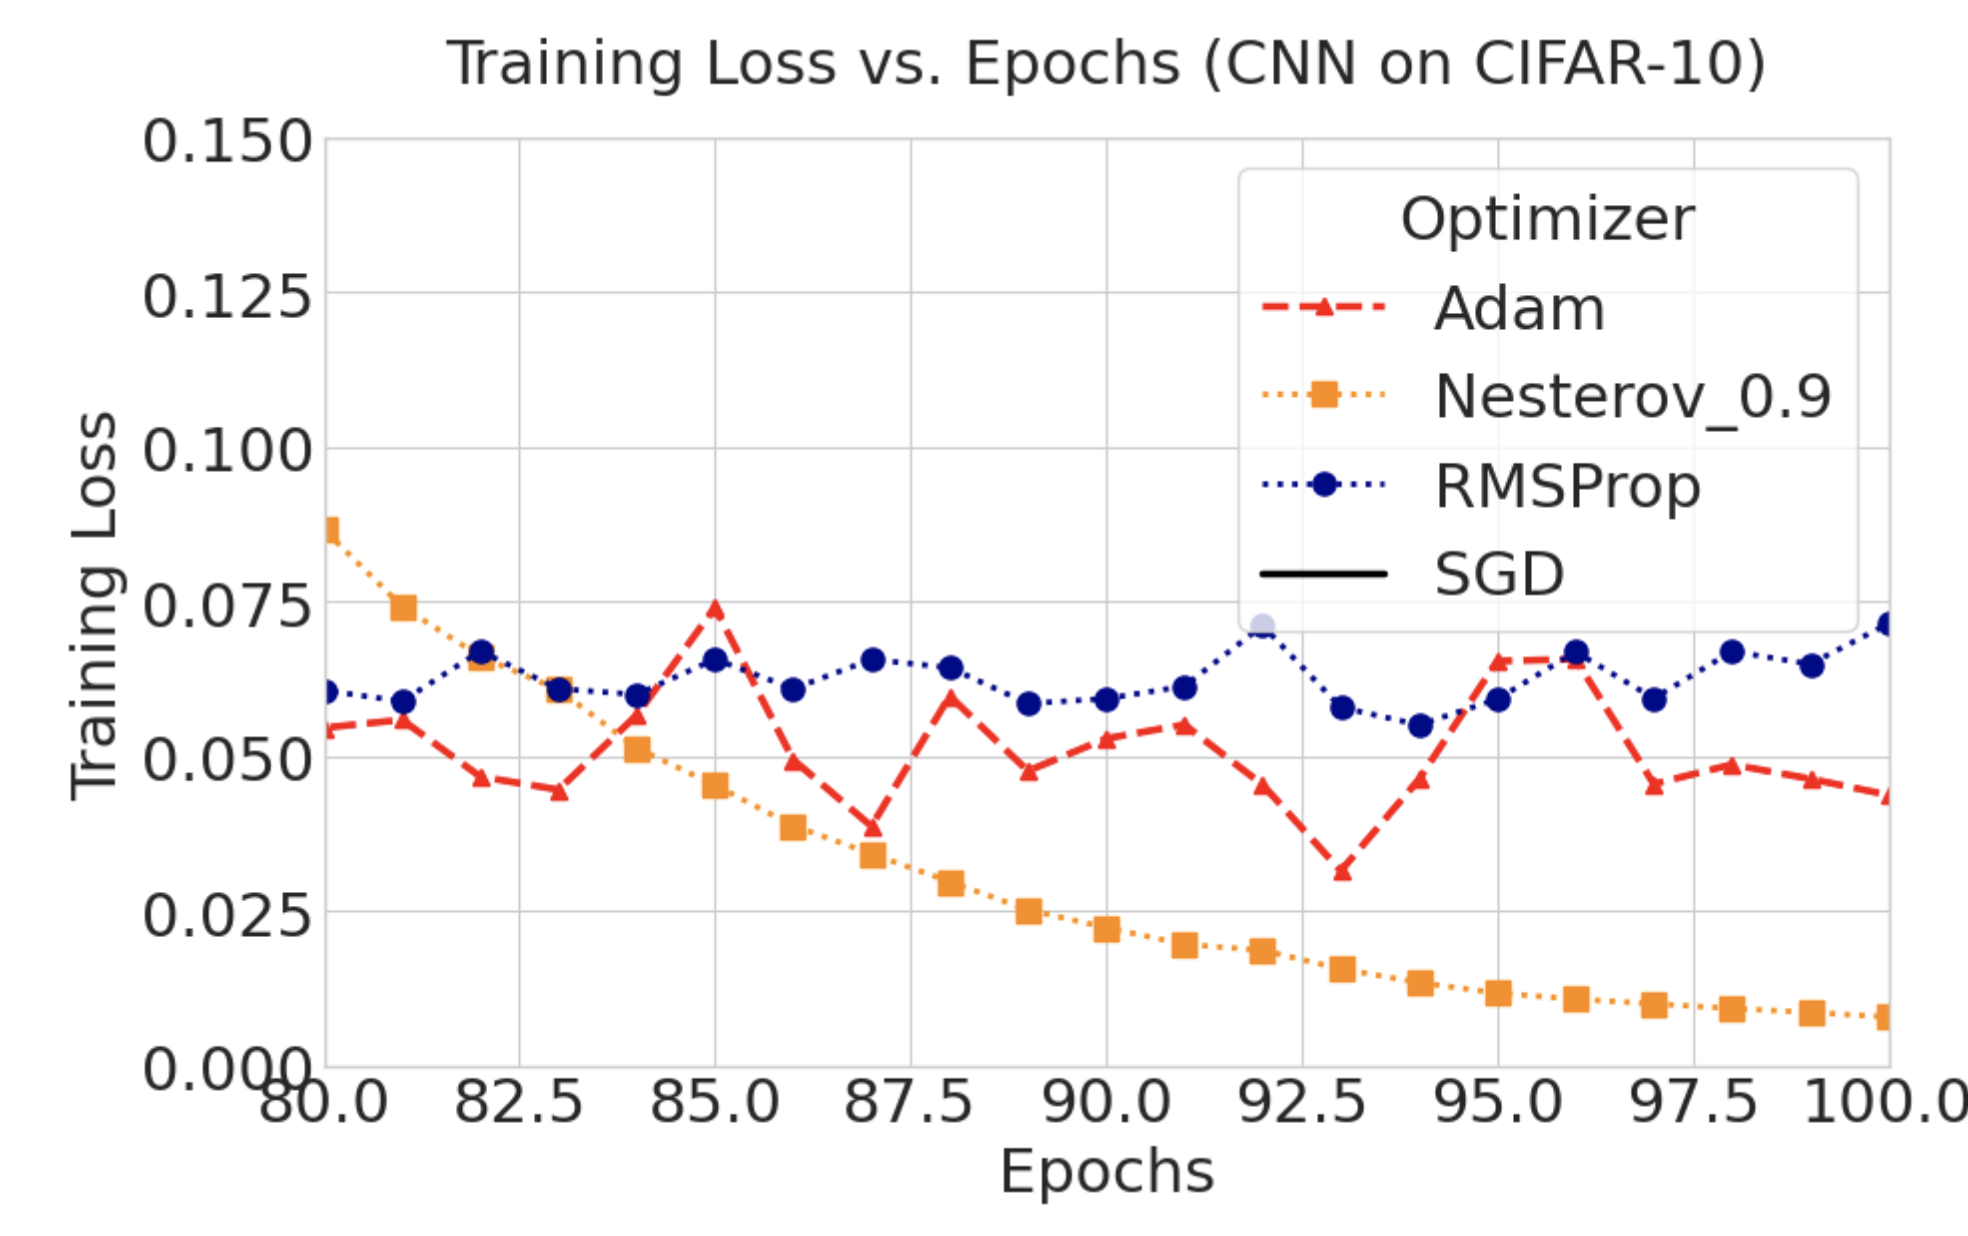
\includegraphics[width=0.45\textwidth]{2-1.png}
    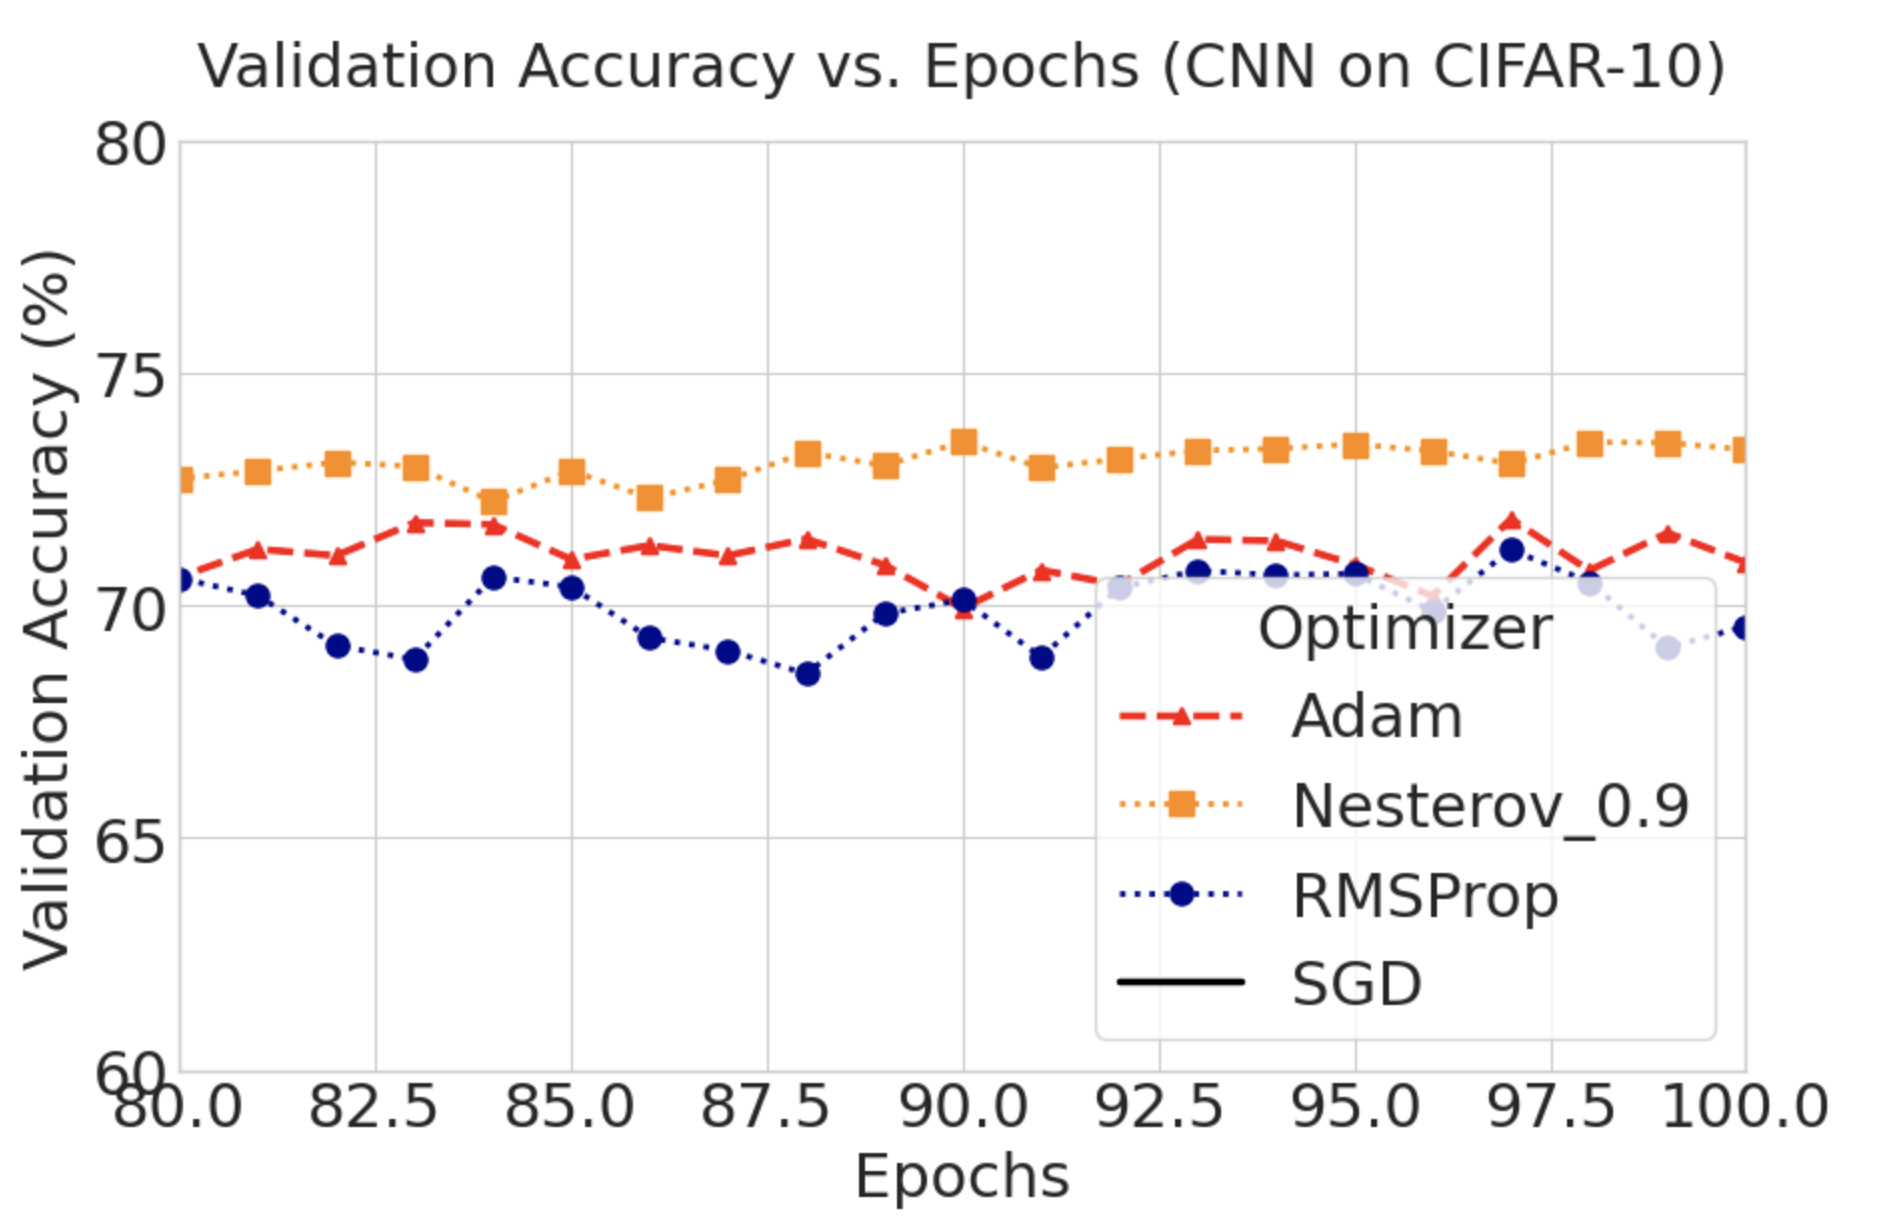
\includegraphics[width=0.45\textwidth]{2-2.png}
    \caption{Detailed plots for epochs 80-100, CNN on CIFAR-10}
    \label{fig:detailed_cnn_on_cifar10}
\end{figure}

The performance from epochs 80-100 shows that Nesterov outperforms Adam and RMSProp in terms of training loss and also achieves better final accuracy. While the performance of the three approaches is very similar from epoch 0-100, a zoomed-in analysis reveals that Nesterov has a better performance at final epochs.

\textbf{Although Nesterov's convergence rate is slower than Adam and RMSProp in the early stages of training, it ultimately achieves lower loss and higher accuracy. It also achieves higher accuracy in the final test, demonstrating Nesterov has better generalization ability on the CNN on CIFAR-10 task.}



\subsubsection{VGG13 on CIFAR-10}

In Figure e, the final loss performance of Adam and Nesterov is highly overlapping; in Figure f, the final accuracy performance of Adam and RMSProp is highly overlapping. We compare their detailed plots for epochs 80-100:

\begin{figure}[H]
    \centering
    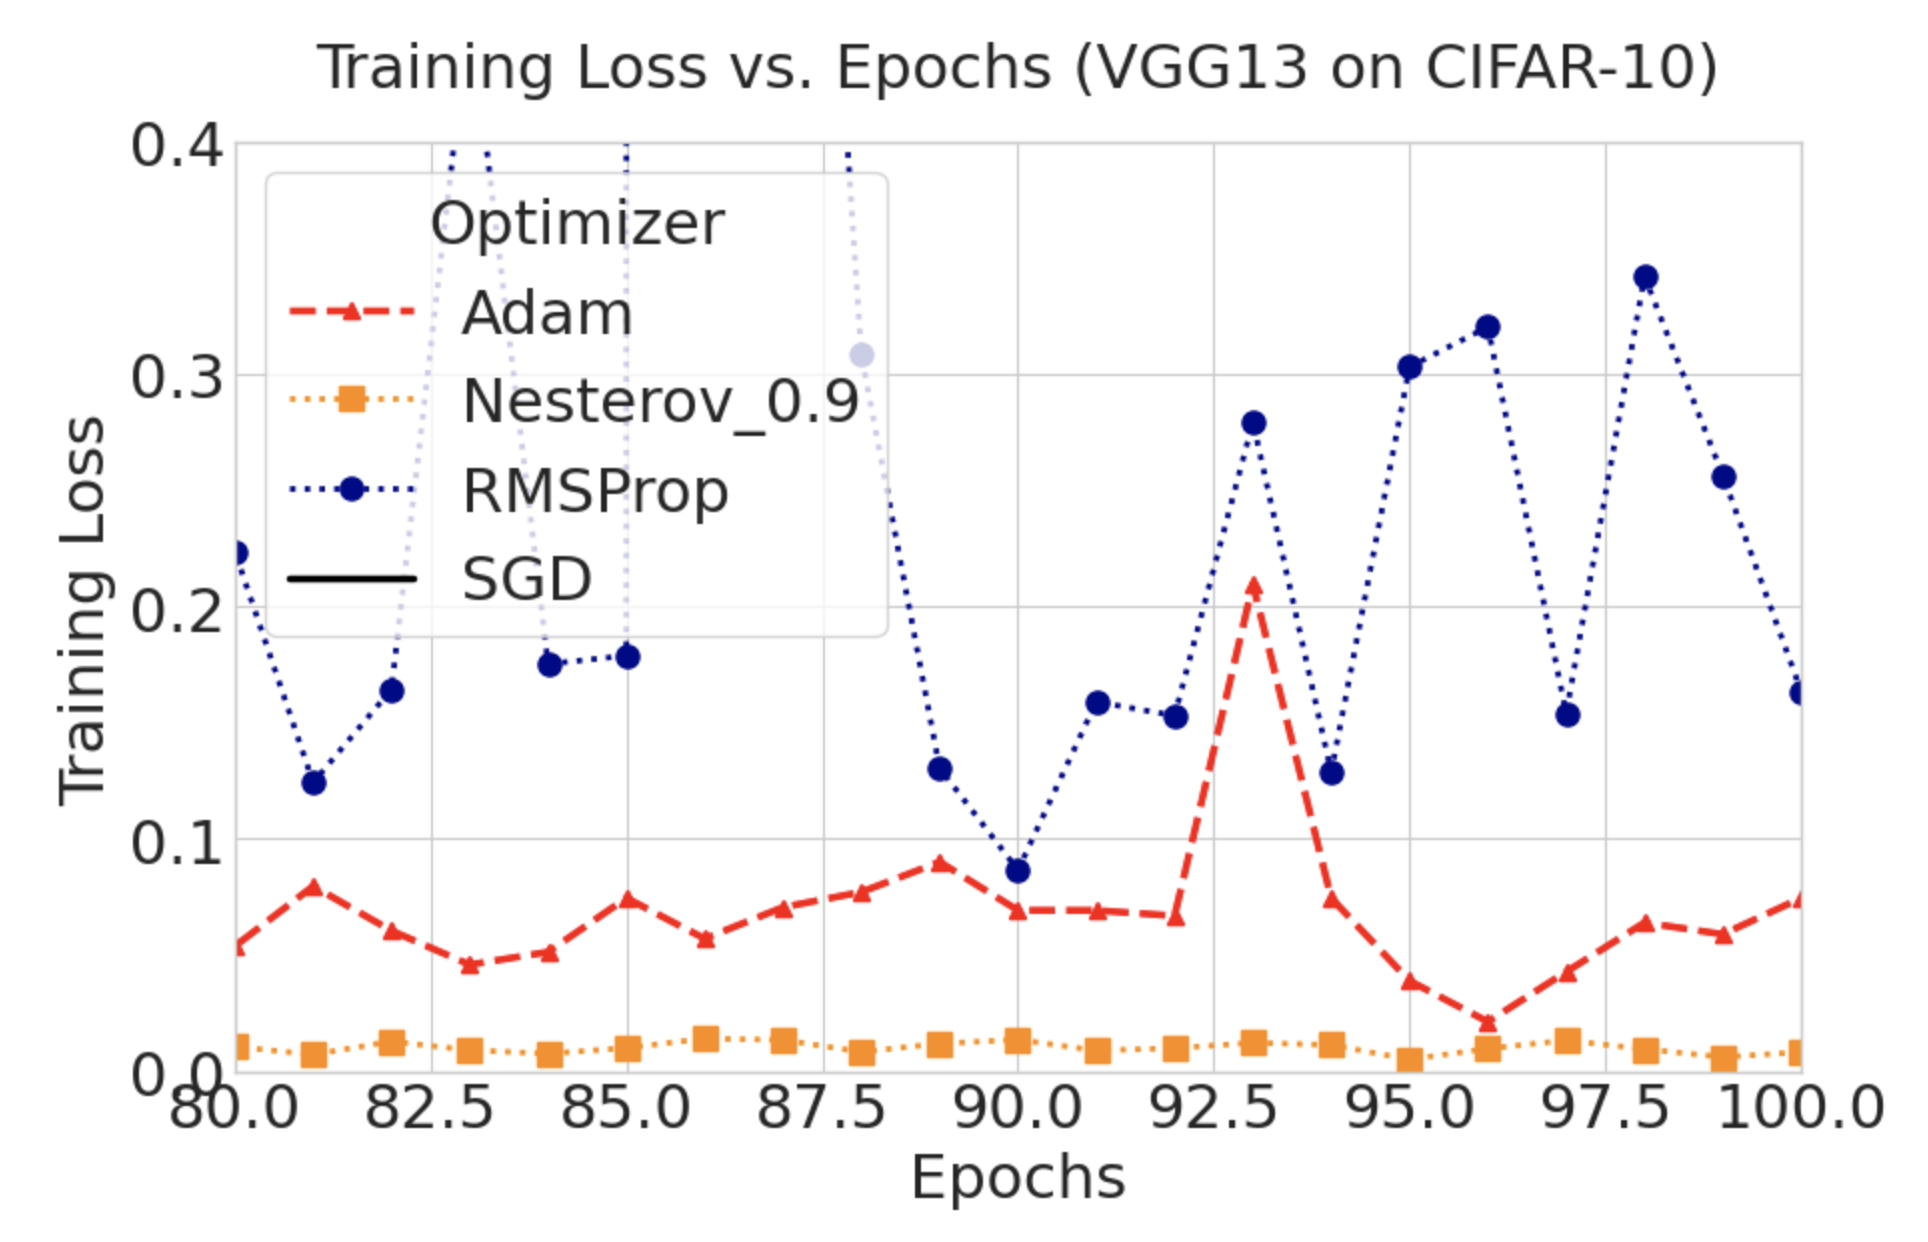
\includegraphics[width=0.45\textwidth]{3-1.png}
    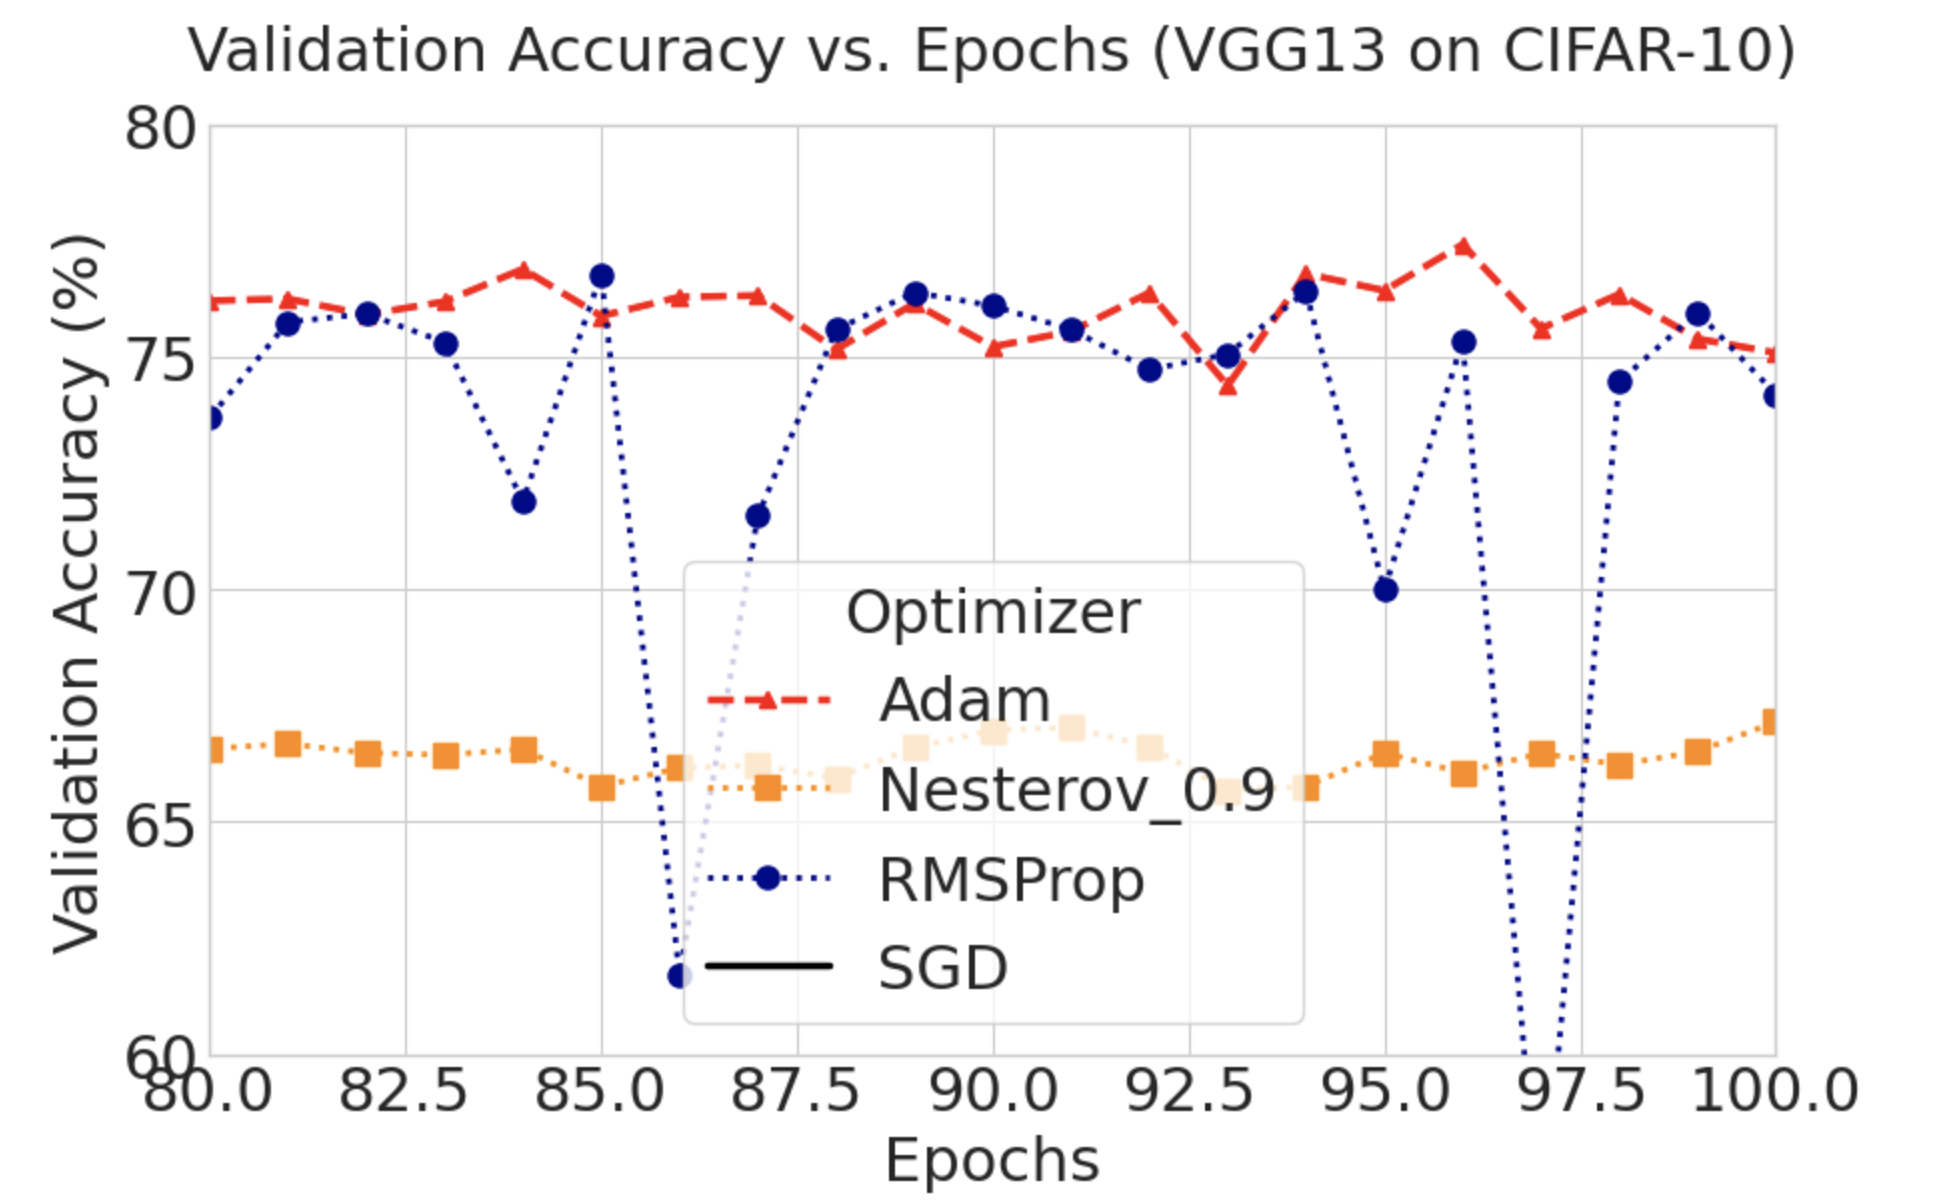
\includegraphics[width=0.45\textwidth]{3-2.png}
    \caption{Detailed plots for epochs 80-100, VGG13 on Cifar10}
    \label{fig:detailed_vgg13_on_cifar10}
\end{figure}

As can be seen from the performance at epochs 80-100, Nesterov's loss performs better, but Adam and RMSProp achieve higher accuracy.

In the first two experiments, the optimizer that converges to a lower loss also achieves better validation accuracy. However, Figure f shows a rather strange result. To rule out other possible influences, I further compared Nesterov's performance under different momentum settings: (See \ref{fig:nesterov_momentum_study}
)




\begin{table}[H]
\centering
\caption{Final Test Accuracy (Nesterov with different momentum)}
\label{tab:nesterov_study}
\begin{tabular}{|l|c|c|c|}
\hline
              & MLP on MNIST & CNN on CIFAR-10 & VGG13 on CIFAR-10 \\ \hline
Nesterov\_0.5  & 93.73\%      & 62.26\%         & 57.07\%           \\ \hline
Nesterov\_0.7  & 95.19\%      & 69.89\%         & 60.98\%           \\ \hline
Nesterov\_0.9  & 97.62\%      & 73.08\%         & 66.43\%           \\ \hline
Nesterov\_0.95 & 97.94\%      & 74.27\%         & 70.11\%           \\ \hline
Nesterov\_0.99 & \textbf{98.05\%} & \textbf{75.34\%}  & \textbf{78.17\%}    \\ \hline
\end{tabular}
\end{table}

From this result, we can see that when Nesterov's momentum is set to 0.99, Nesterov outperforms Adam and RMSProp on the final test set.

Therefore, in the VGG13 on CIFAR-10 experiment, \textbf{Nesterov converged more slowly than Adam and RMSProp, but ultimately converged to a lower loss level. When Nesterov's momentum was set to the commonly used 0.9, its validation and test accuracy were lower than Adam and RMSProp. However, when the momentum was set to 0.99, Nesterov performed even better on the test set. Therefore, Nesterov with a momentum of 0.99 performed best on the VGG13 on CIFAR-10 task.}

%%%%%%%%%%%%%%%%%%%%%%%%%%%%%%%%%%%
\subsection{Comprehensive Comparison and Discussion}

Let's see all six methods:


\begin{figure}[htbp]
    \centering
    % MLP row
    \subfloat[MLP Training Loss on MNIST]{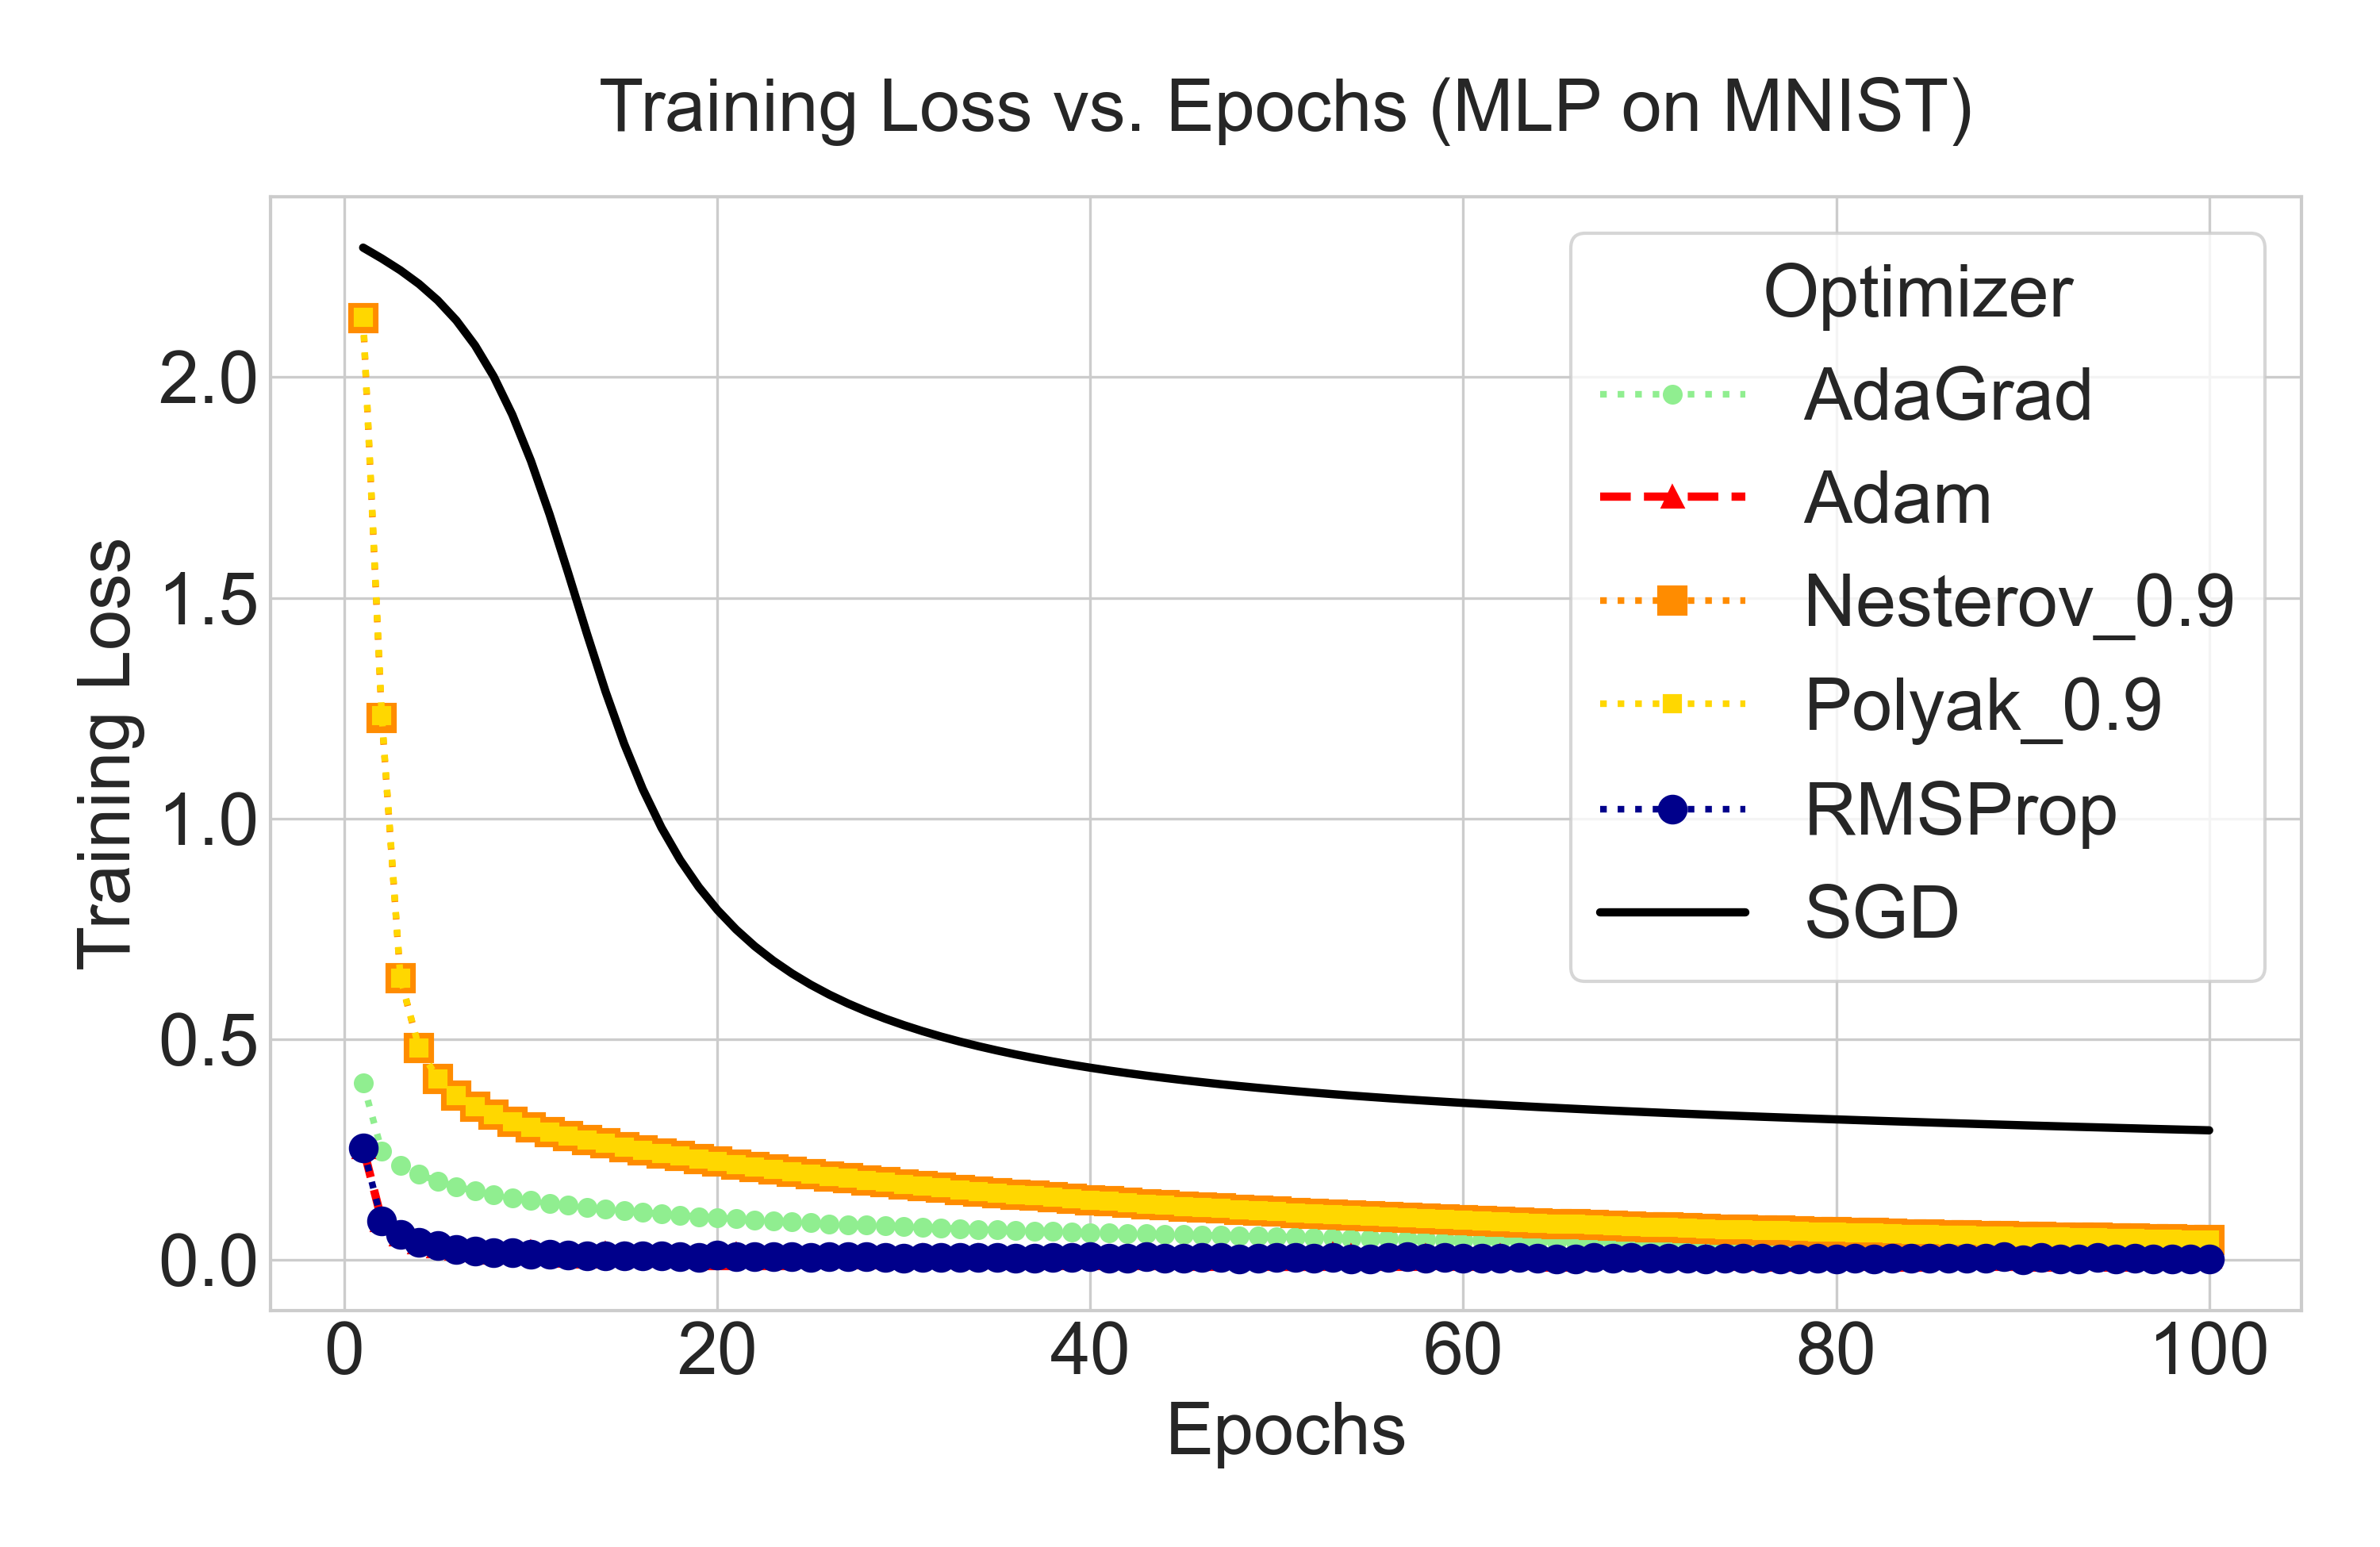
\includegraphics[width=0.48\textwidth]{Analysis_5_Comprehensive_Comparison1_mnist_mlp_training_loss.png}} \quad
    \subfloat[MLP Validation Accuracy on MNIST]{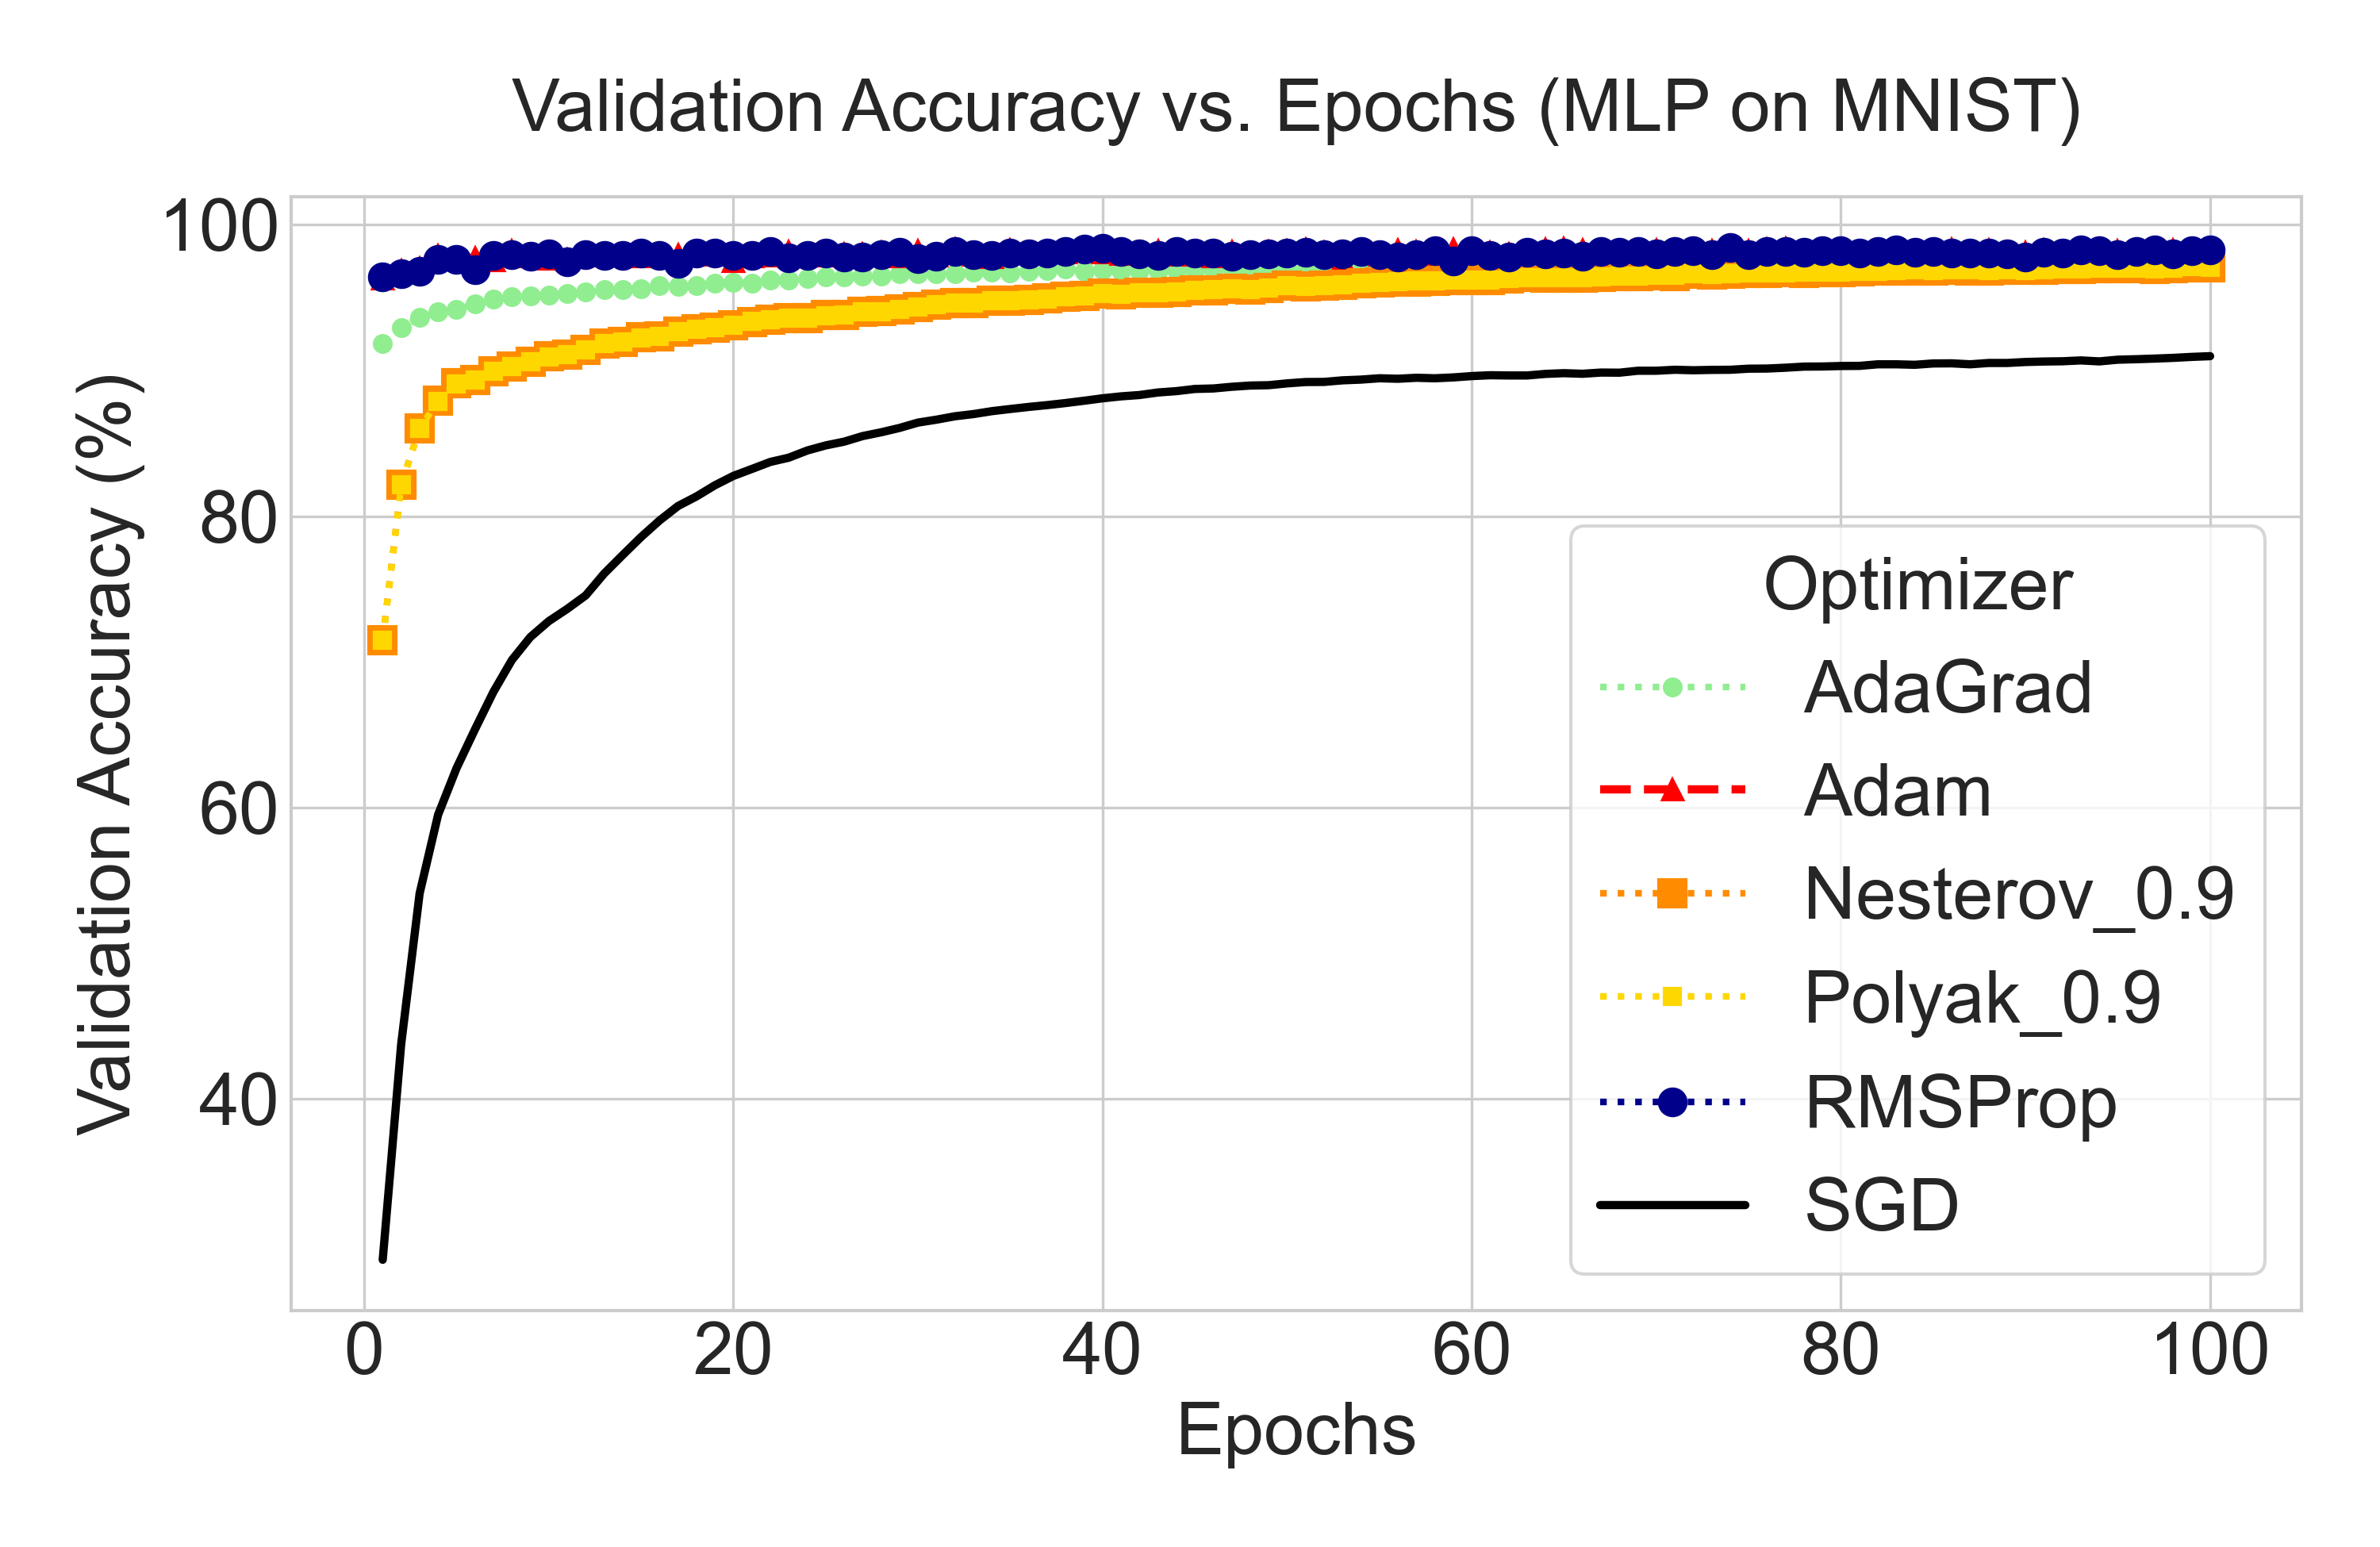
\includegraphics[width=0.48\textwidth]{Analysis_5_Comprehensive_Comparison1_mnist_mlp_validation_accuracy.png}} \\
    % CNN row
    \subfloat[CNN Training Loss on CIFAR-10]{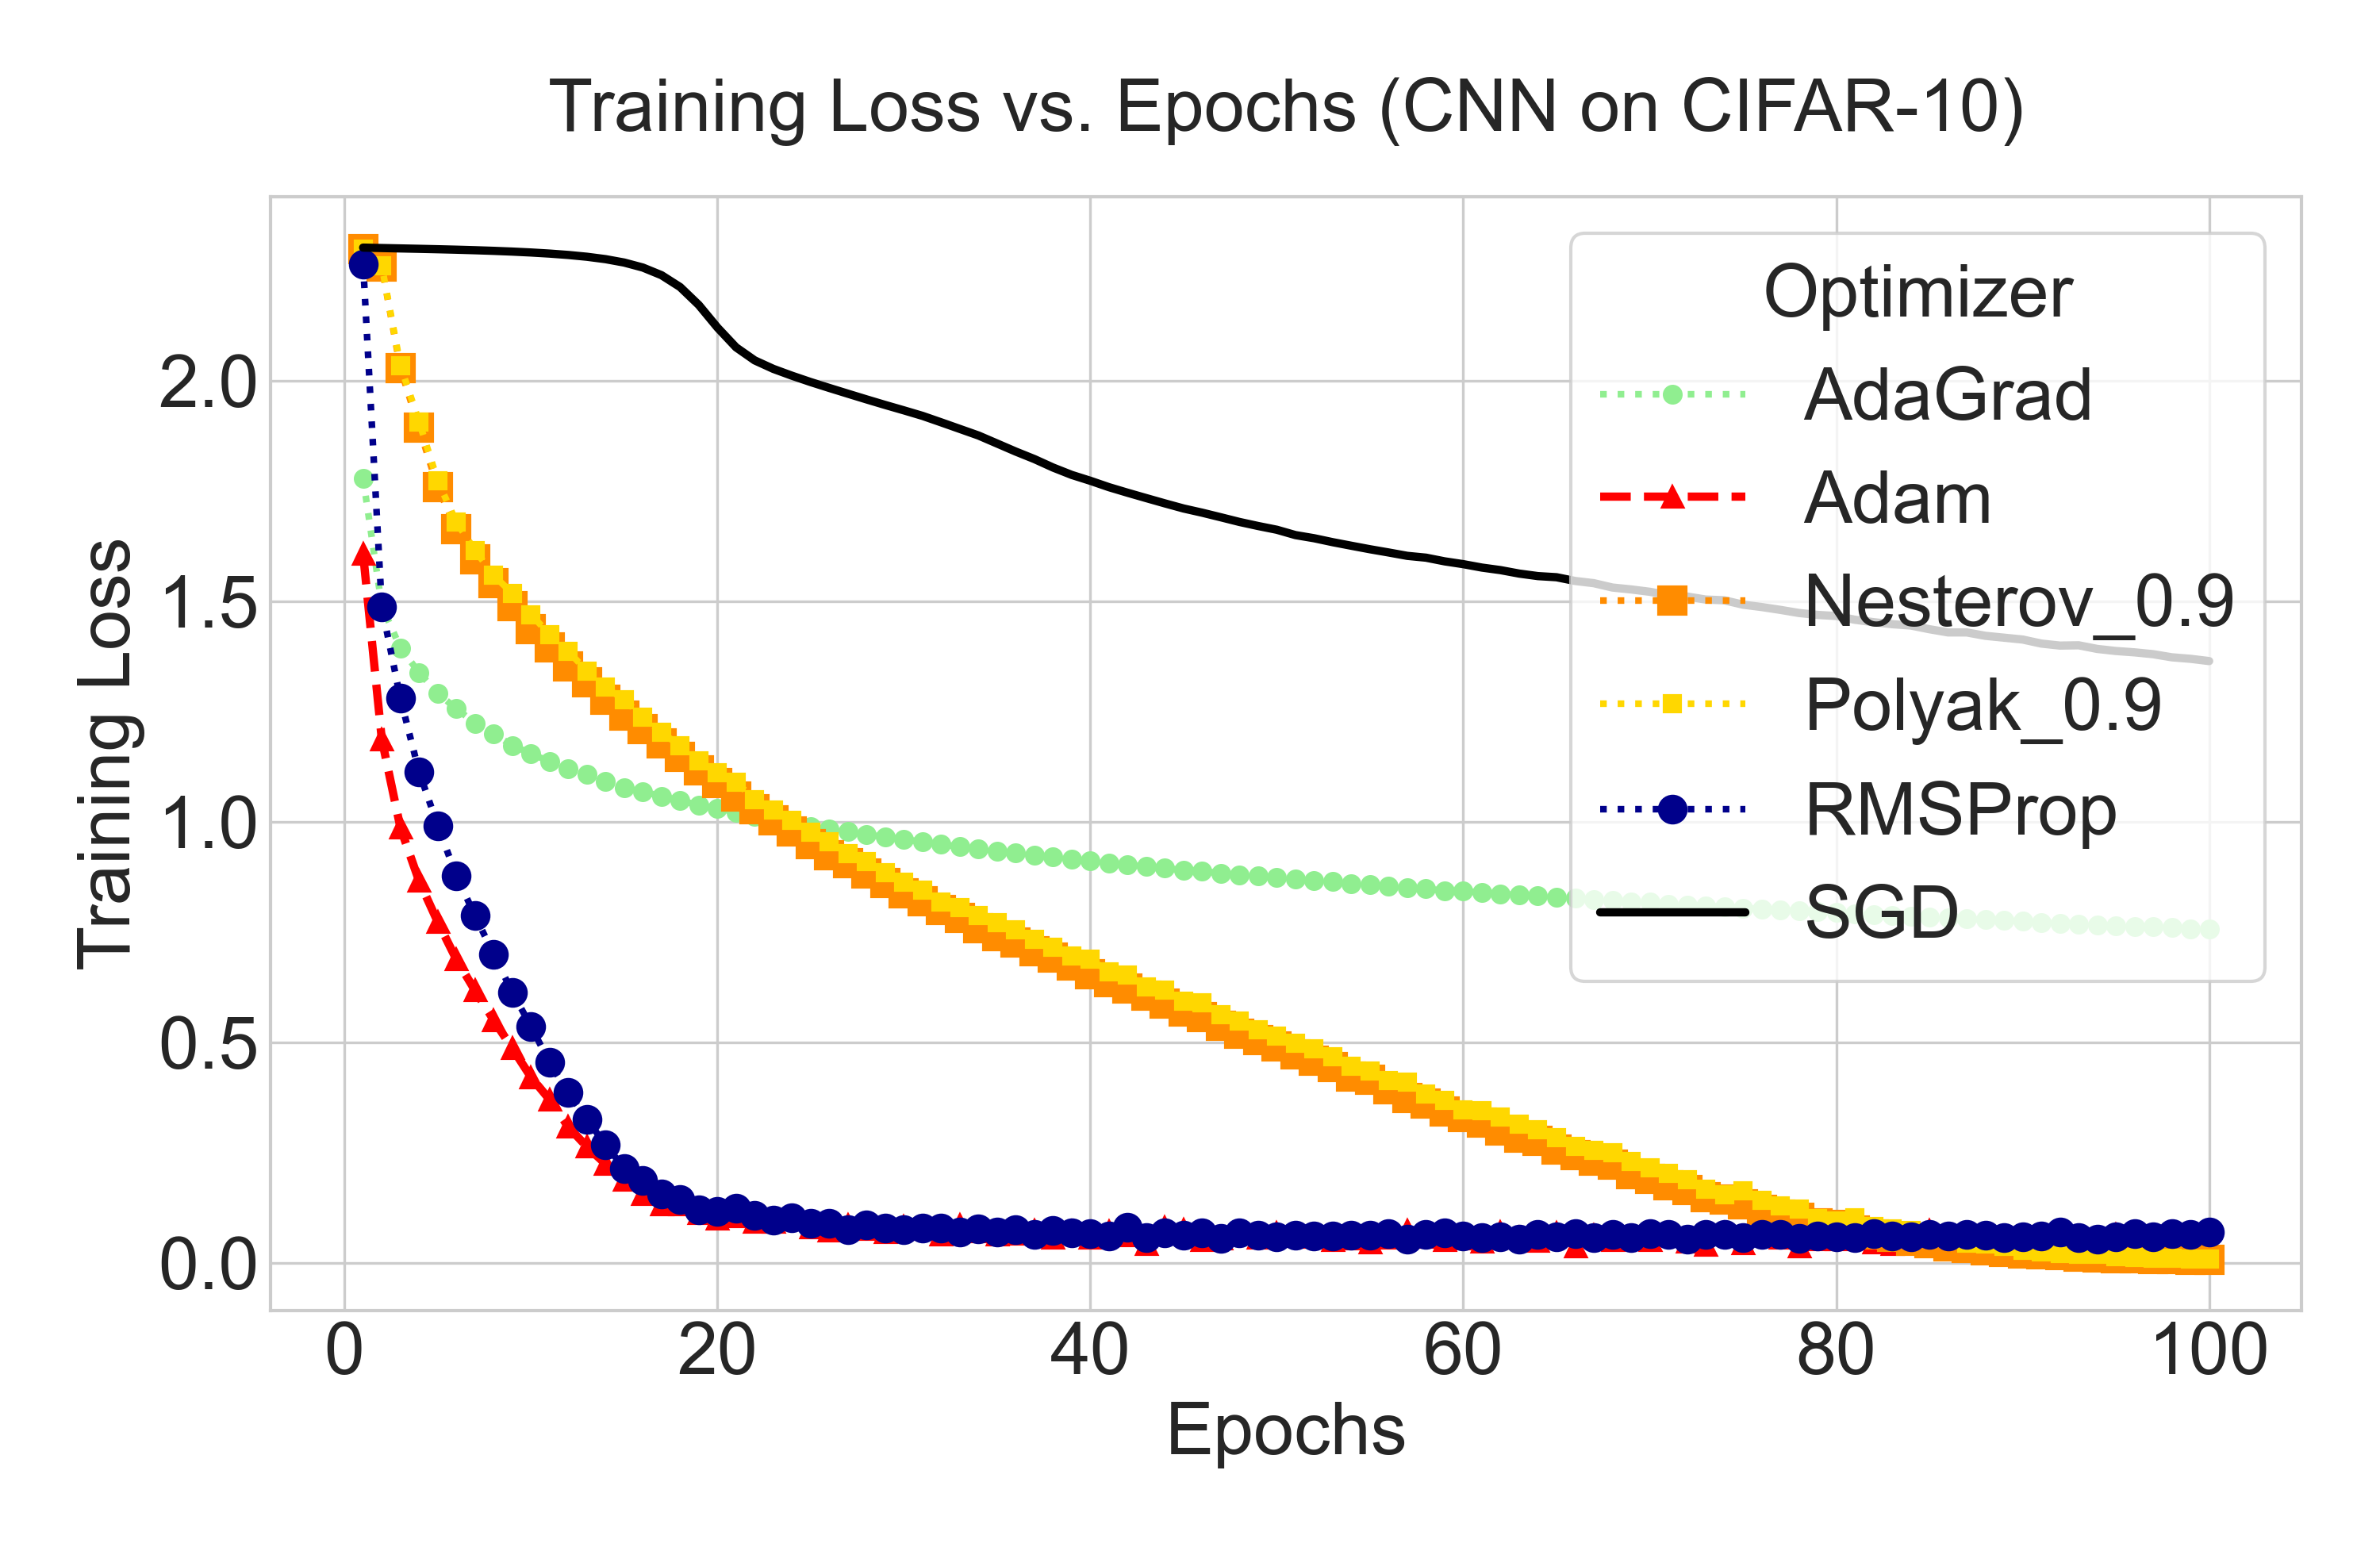
\includegraphics[width=0.48\textwidth]{Analysis_5_Comprehensive_Comparison2_cifar10_cnn_training_loss.png}} \quad
    \subfloat[CNN Validation Accuracy on CIFAR-10]{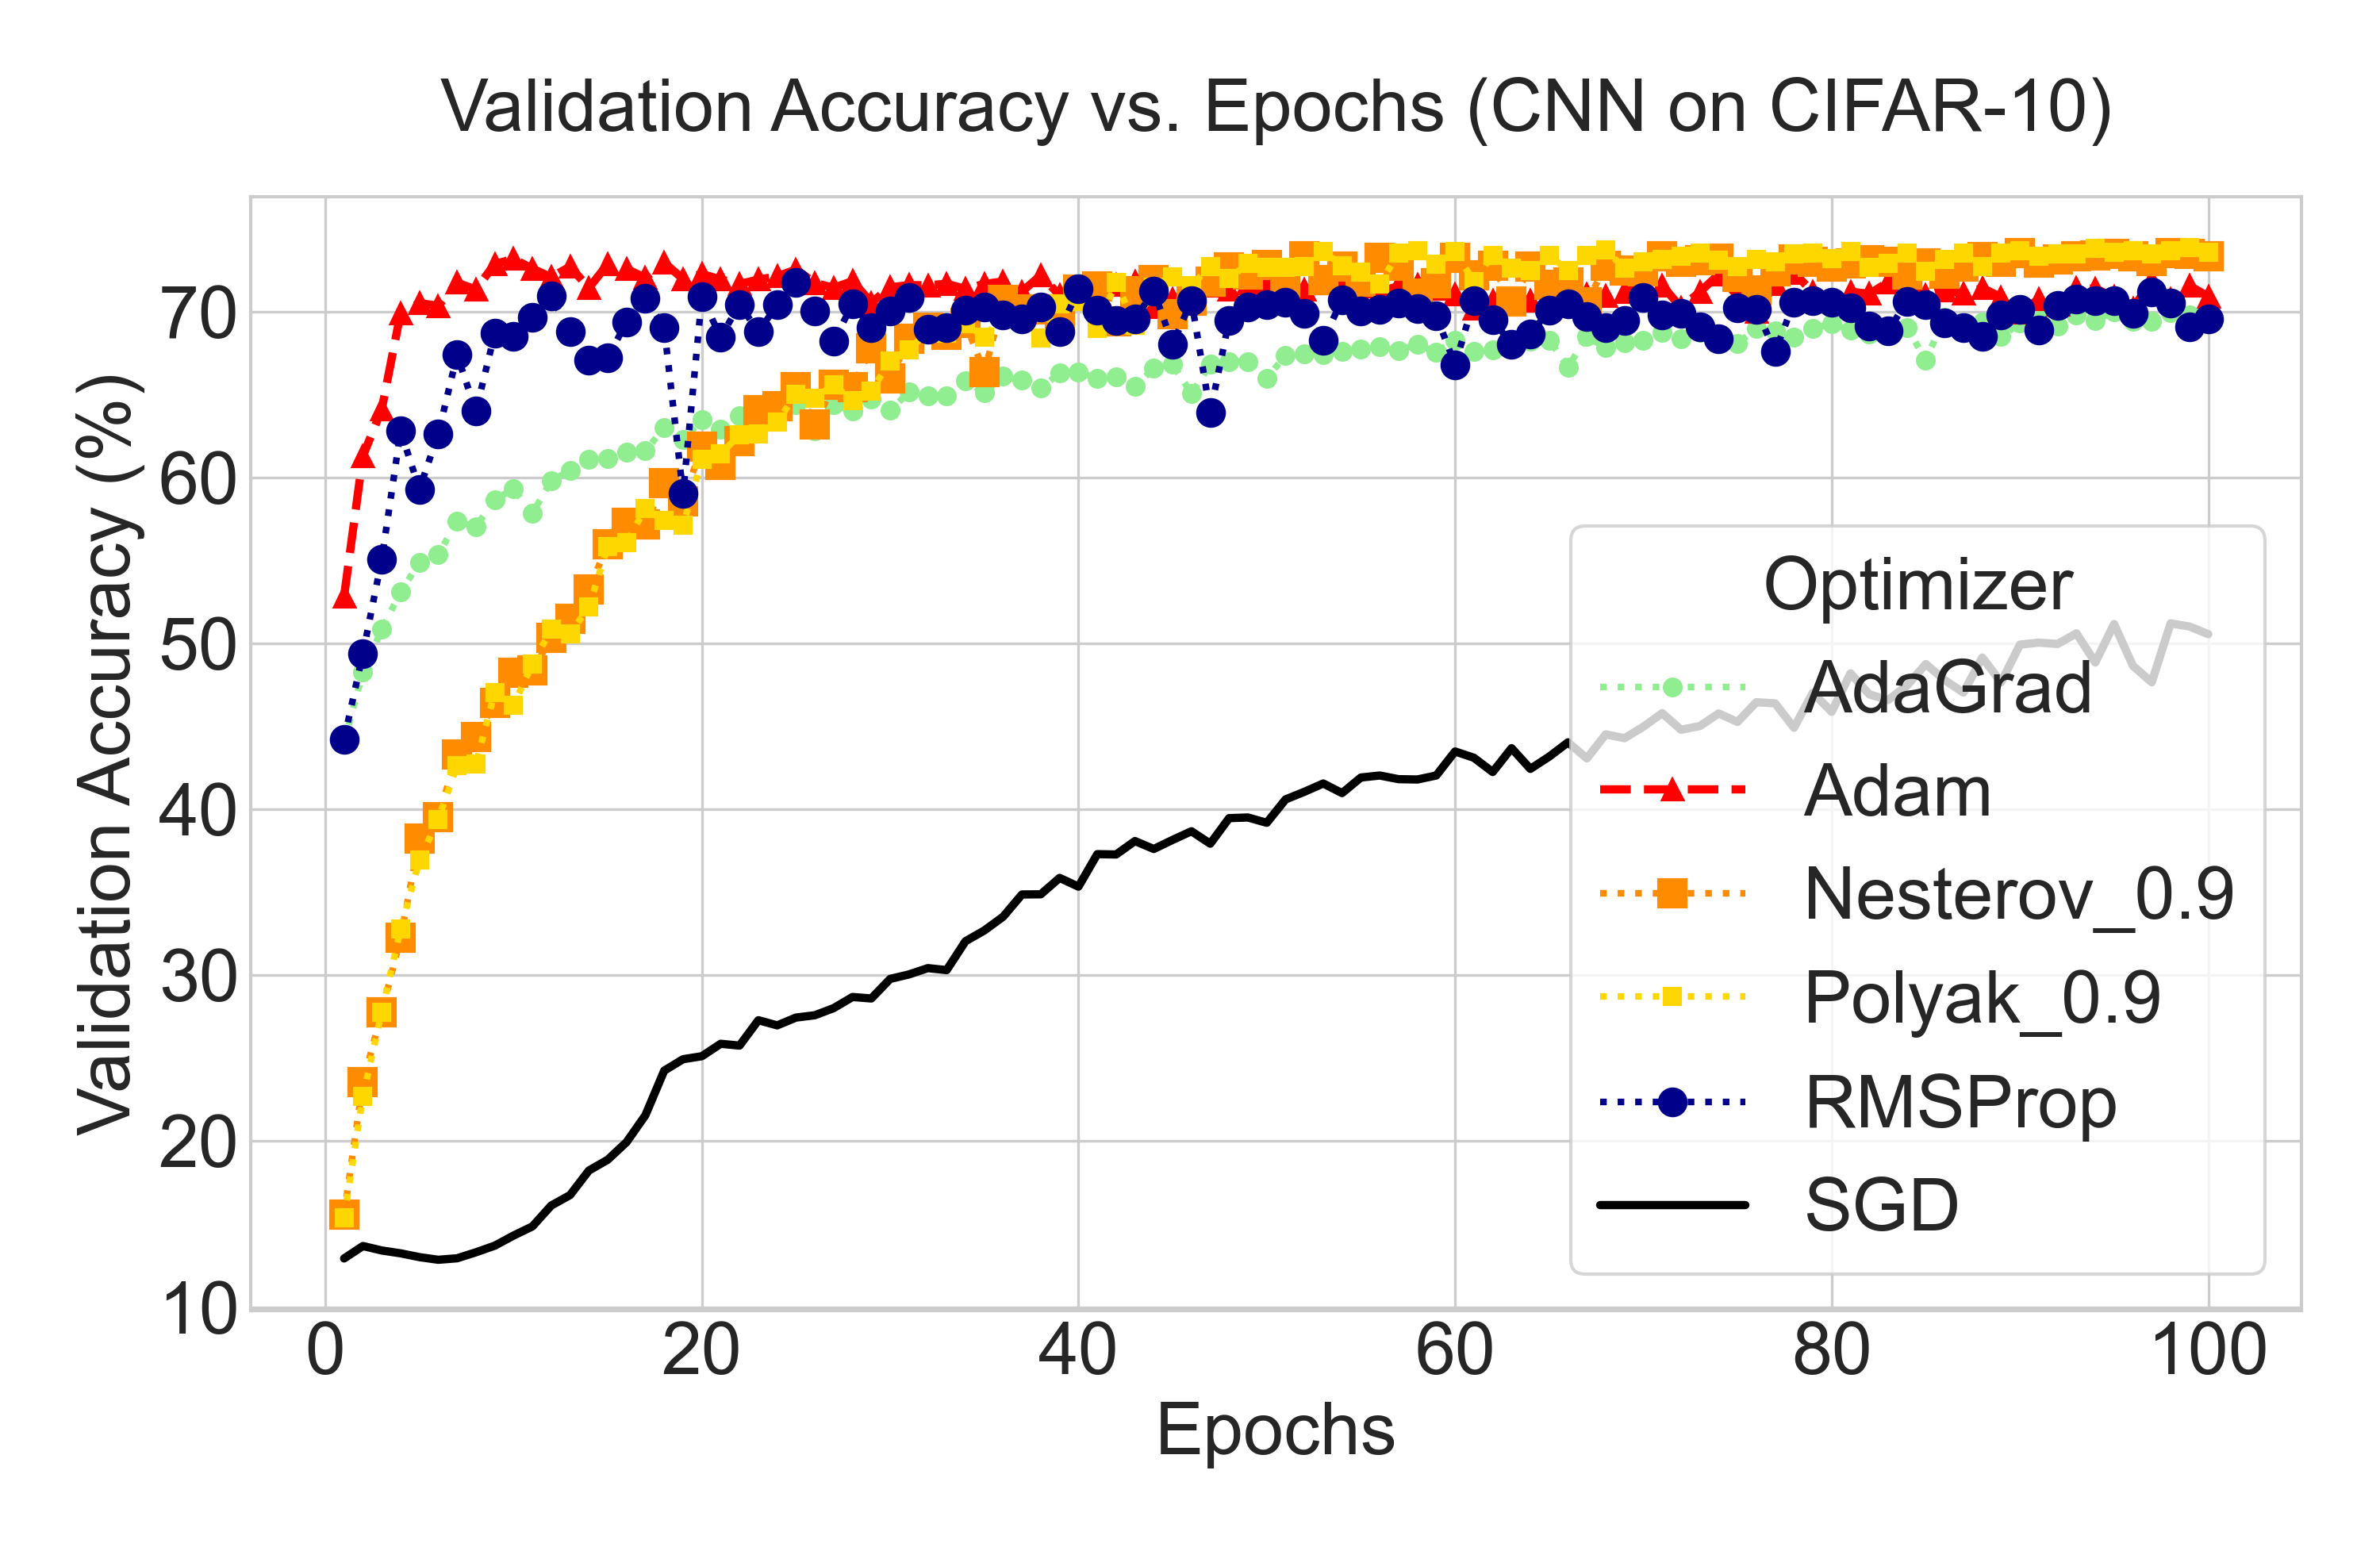
\includegraphics[width=0.48\textwidth]{Analysis_5_Comprehensive_Comparison2_cifar10_cnn_validation_accuracy.png}} \\
    % VGG13 row
    \subfloat[VGG13 Training Loss on CIFAR-10]{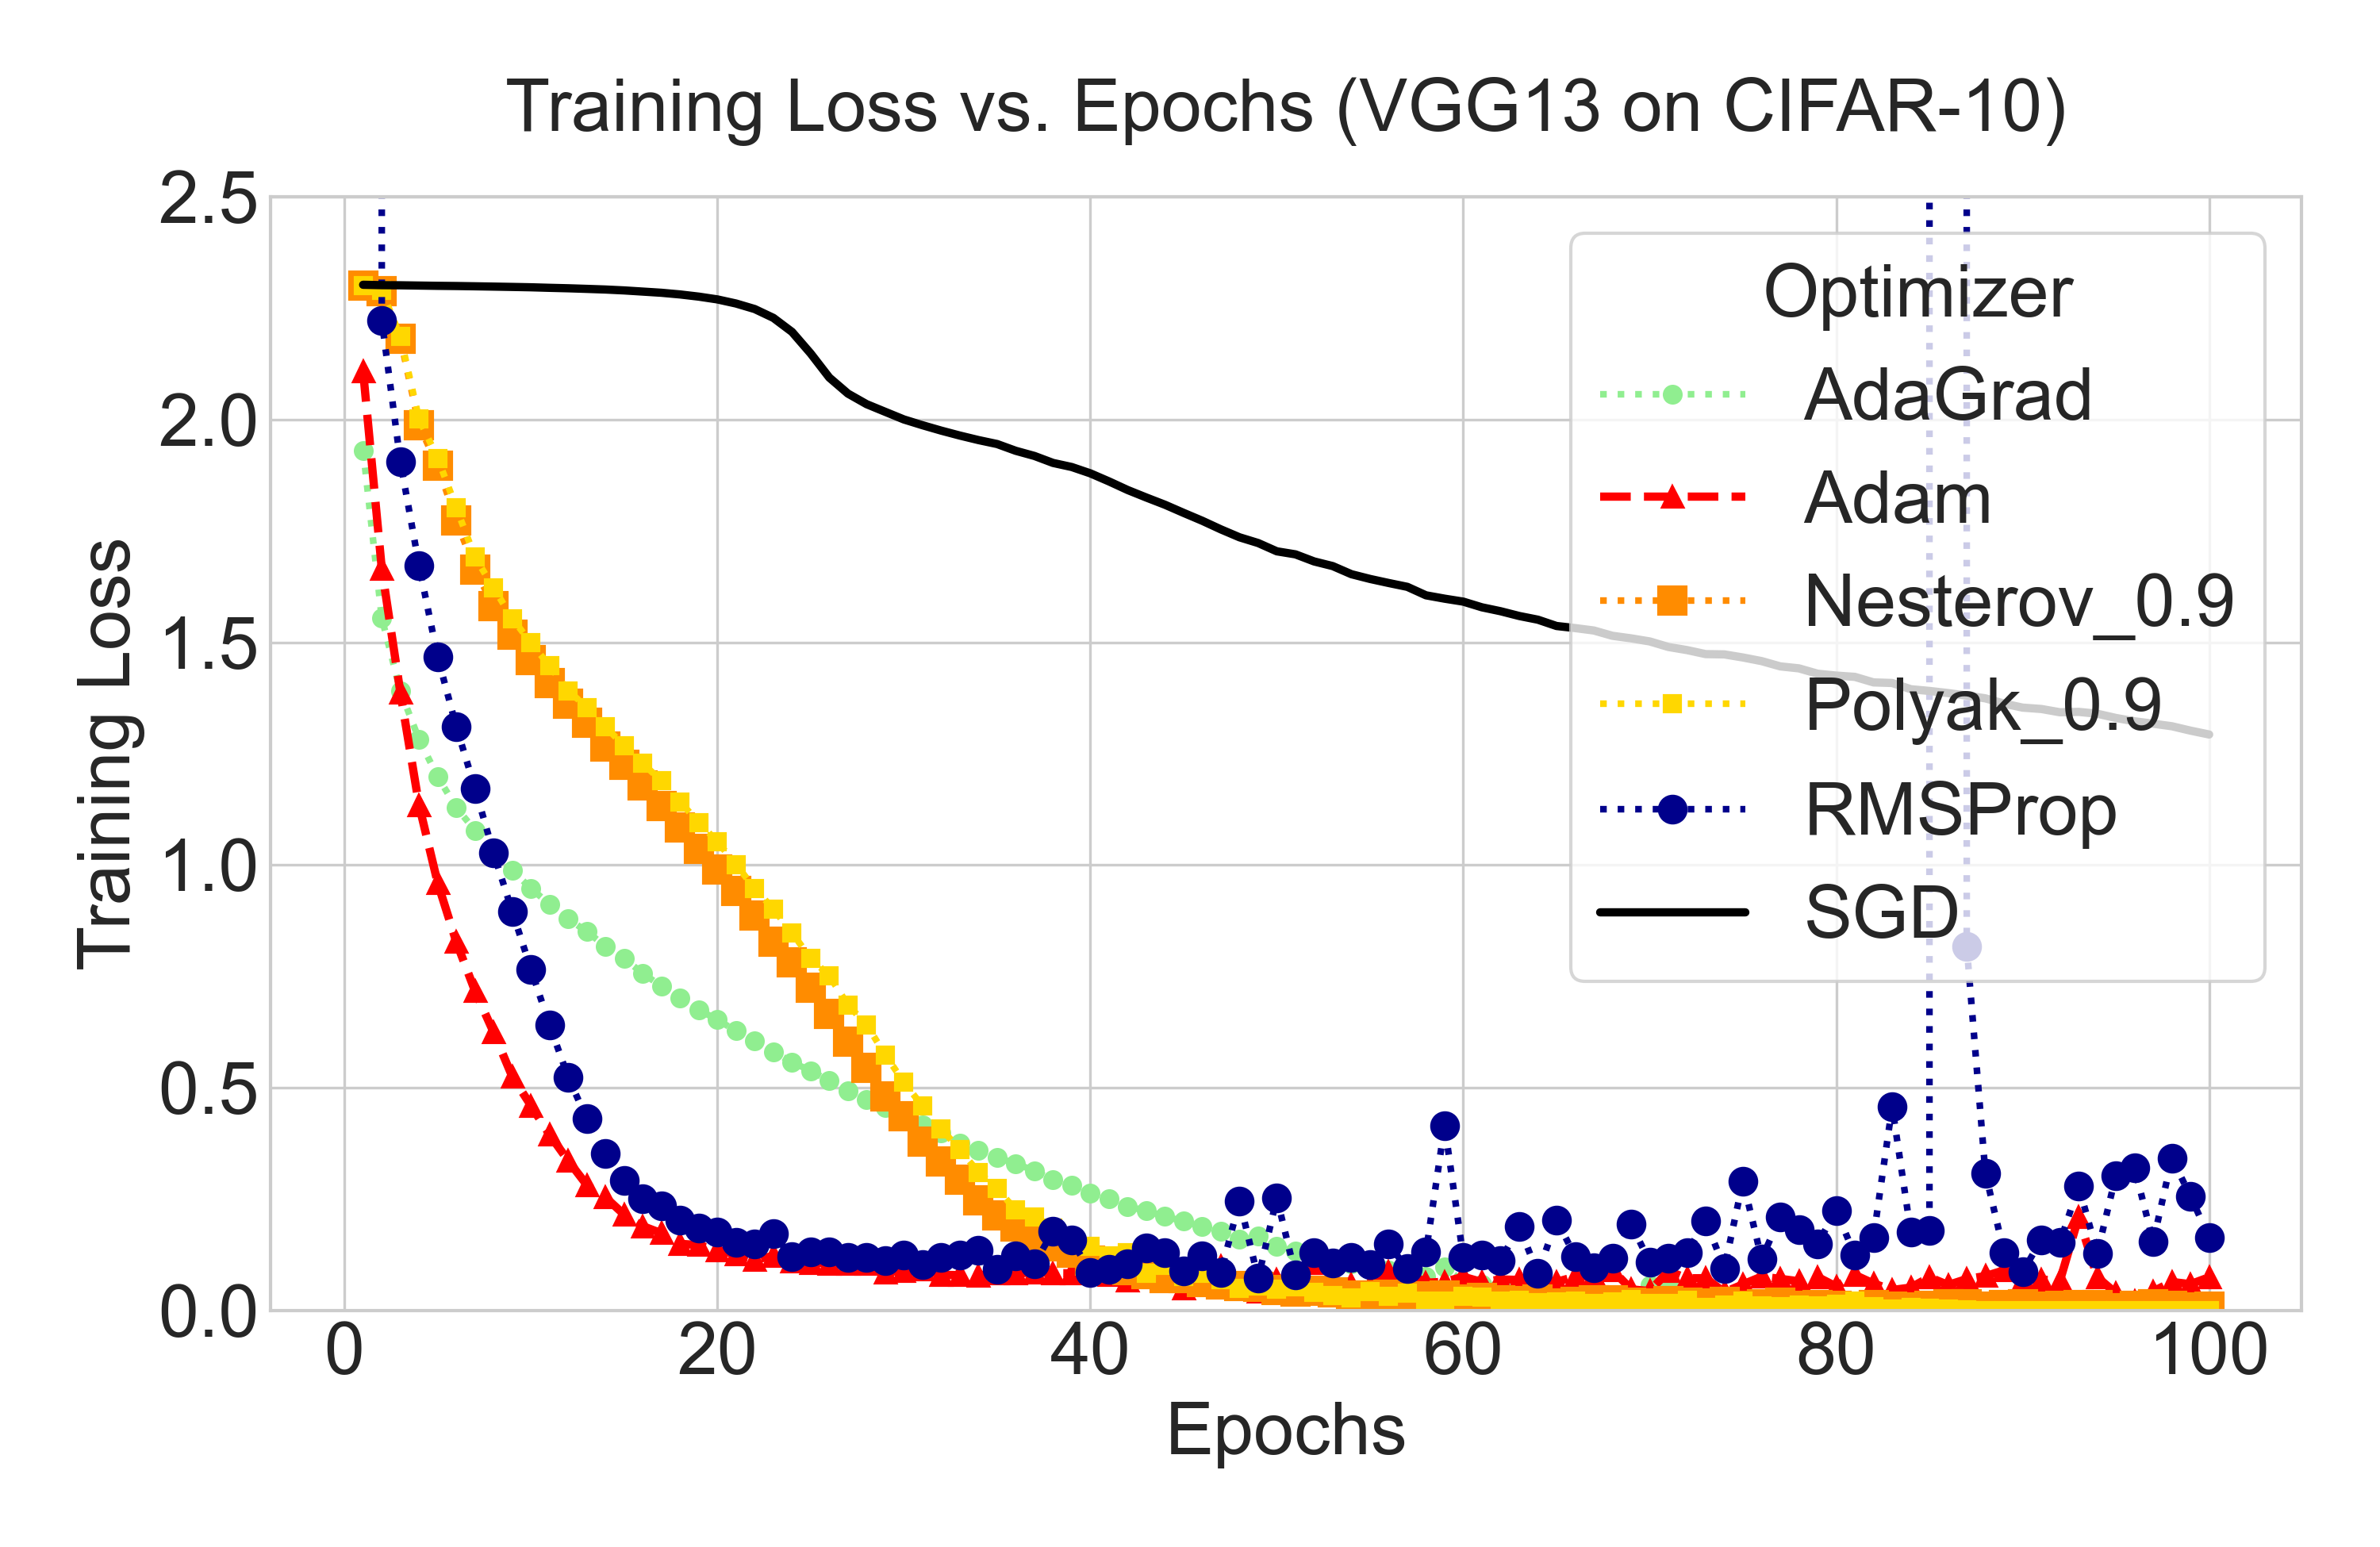
\includegraphics[width=0.48\textwidth]{Analysis_5_Comprehensive_Comparison3_cifar_vgg13_training_loss.png}} \quad
    \subfloat[VGG13 Validation Accuracy on CIFAR-10]{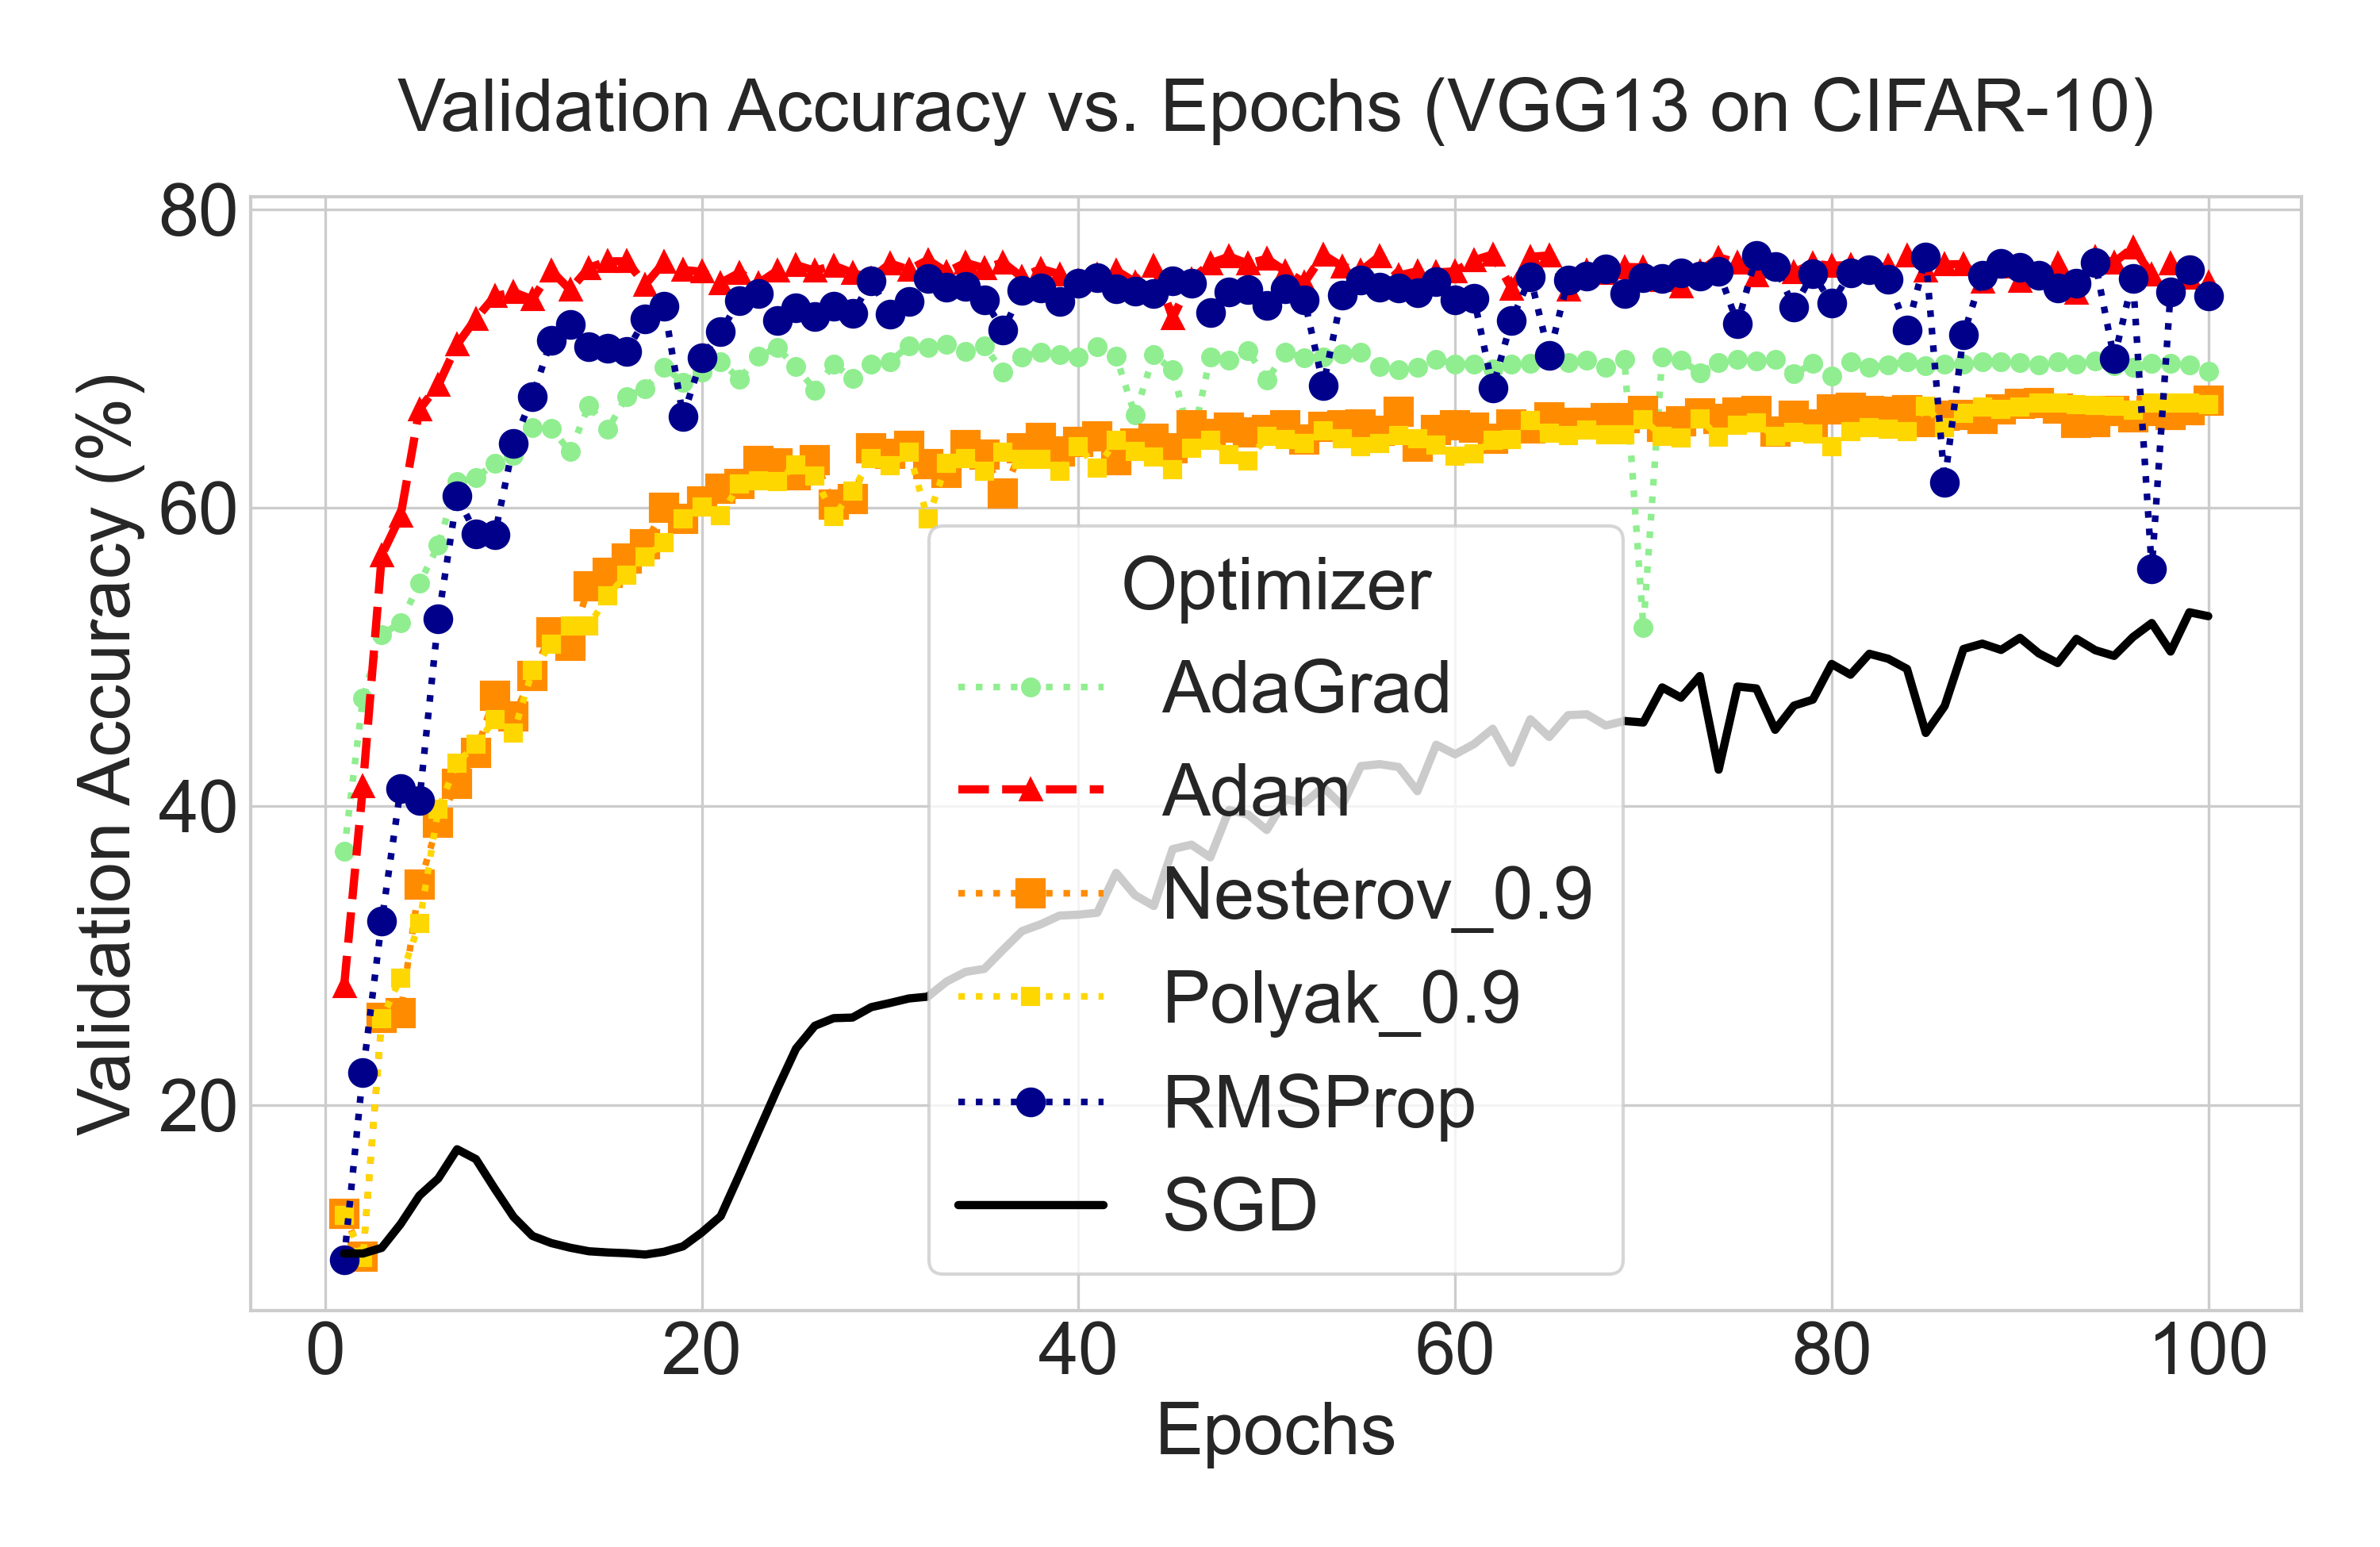
\includegraphics[width=0.48\textwidth]{Analysis_5_Comprehensive_Comparison3_cifar_vgg13_validation_accuracy.png}}
    \caption{Comprehensive performance comparison of all optimization algorithms: SGD (black), AdaGrad (green), RMSProp (blue), Nesterov (orange), and Adam (red)}
    \label{fig:comprehensive_comparison_final}
\end{figure}


\begin{table}[H]
\centering
\caption{Comprehensive Comparison: Final Test Accuracy of All Optimizers}
\label{tab:comprehensive_comparison}
\begin{tabular}{|l|c|c|c|}
\hline
             & MLP on MNIST & CNN on CIFAR-10 & VGG13 on CIFAR-10 \\ \hline
SGD          & 91.82\%      & 50.64\%         & 52.68\%           \\ \hline
AdaGrad      & 97.77\%      & 69.98\%         & 68.11\%           \\ \hline
RMSProp      & 98.29\%      & 68.65\%         & 73.61\%           \\ \hline
Adam         & \textbf{98.32\%} & 70.15\%         & \textbf{74.61\%}    \\ \hline
Polyak\_0.9   & 97.64\%      & \textbf{73.00\%}  & 65.75\%           \\ \hline
Nesterov\_0.9 & 97.62\%      & 72.91\%         & 66.02\%           \\ \hline
\end{tabular}
\end{table}

I also compared the test accuracy of Polyak under different momentum settings and found that, like Nesterov, it performed best when the momentum value was set to 0.99:

\begin{table}[H]
\centering
\caption{Final Test Accuracy (Polyak with different momentum)}
\label{tab:polyak_study}
\begin{tabular}{|l|c|c|c|}
\hline
             & MLP on MNIST & CNN on CIFAR-10 & VGG13 on CIFAR-10 \\ \hline
Polyak\_0.5   & 93.75\%      & 62.34\%         & 59.15\%           \\ \hline
Polyak\_0.7   & 95.19\%      & 69.44\%         & 60.12\%           \\ \hline
Polyak\_0.9   & 97.64\%      & 73.10\%         & 65.04\%           \\ \hline
Polyak\_0.95  & 97.94\%      & 74.02\%         & 68.32\%           \\ \hline
Polyak\_0.99  & \textbf{98.06\%} & \textbf{76.30\%}  & \textbf{74.83\%}    \\ \hline
\end{tabular}
\end{table}

Now, let's add Polyak and Nesterov optimal momentum selection to the comparison and make a comprehensive comparison of the six optimizers we learned:

\begin{table}[H]
\centering
\caption{Final Test Accuracy with Best Performance' Momentum Settings}
\label{tab:comprehensive_comparison}
\begin{tabular}{|l|c|c|c|}
\hline
             & MLP on MNIST & CNN on CIFAR-10 & VGG13 on CIFAR-10 \\ \hline
SGD          & 91.82\%      & 50.64\%         & 52.68\%           \\ \hline
AdaGrad      & 97.77\%      & 69.98\%         & 68.11\%           \\ \hline
RMSProp      & 98.29\%      & 68.65\%         & 73.61\%           \\ \hline
Adam         & \textbf{98.32\%} & 70.15\%         & 74.61\%    \\ \hline
Polyak\_0.99   & 98.06\%      & \textbf{76.30\%}  & 74.83\%           \\ \hline
Nesterov\_0.99 & 98.05\%      & 75.34\%         & \textbf{78.17\%}           \\ \hline
\end{tabular}
\end{table}

Now, we can conduct a comprehensive experimental summary:

\textbf{(1) Optimizers using adaptive gradient or momentum outperform baseline SGD.}

\textbf{(2) In the MLP on MNIST task, Adam and RMSProp perform best in training and have the best generalization ability. Adam has the best test accuracy, but RMSProp also performs close to Adam's level.}

\textbf{(3) In the CNN on CIFAR-10 task, Nesterov converges slower than Adam and RMSProp, but has a lower final loss.} When we set the momentum to 0.99, Nesterov performs best in test accuracy. In Appendix 1, I added Polyak for comparison and found that Polyak performs best when the momentum is set to 0.99. \textbf{Therefore, in this task, the momentum method performs best, and Polyak (0.99) has the highest test accuracy. }

\textbf{(4) In the VGG13 on CIFAR-10 task, Nesterov converges slower than Adam and RMSProp, but achieves lower final loss.} When we set Nesterov's momentum to 0.99, Nesterov achieves the best performance in terms of test accuracy. \textbf{Therefore, Nesterov is the best optimizer in this task.}

%%%%%%%%%%%%%%%%%%%%%%%%%%%%%%%%
\section{Conclusion}

Through the above experiments, we can see that \textbf{different optimizers have different performance in different tasks, and no single optimizer can achieve the best performance across all tasks.}

Furthermore, the momentum method exhibits distinct performance under different momentum settings, demonstrating that \textbf{the same optimizer can also perform differently under different hyperparameter settings.}

Thus, this experiment provides a valuable conclusion for deep learning training: when we are going to train a new deep learning task, \textbf{we should first explore different optimizers and explore different hyperparameter settings for the same optimizer to preliminarily identify the optimizer that is most suitable for the task.}

%%%%%%%%%%%%%%%%%%%%%%%%%%%%%%%%%%%
\clearpage
\section*{Appendix}
\subsection*{(a) Nesterov Momentum}
\begin{figure}[htbp]
    \centering
    % MLP row
    \subfloat[MLP Loss on MNIST]{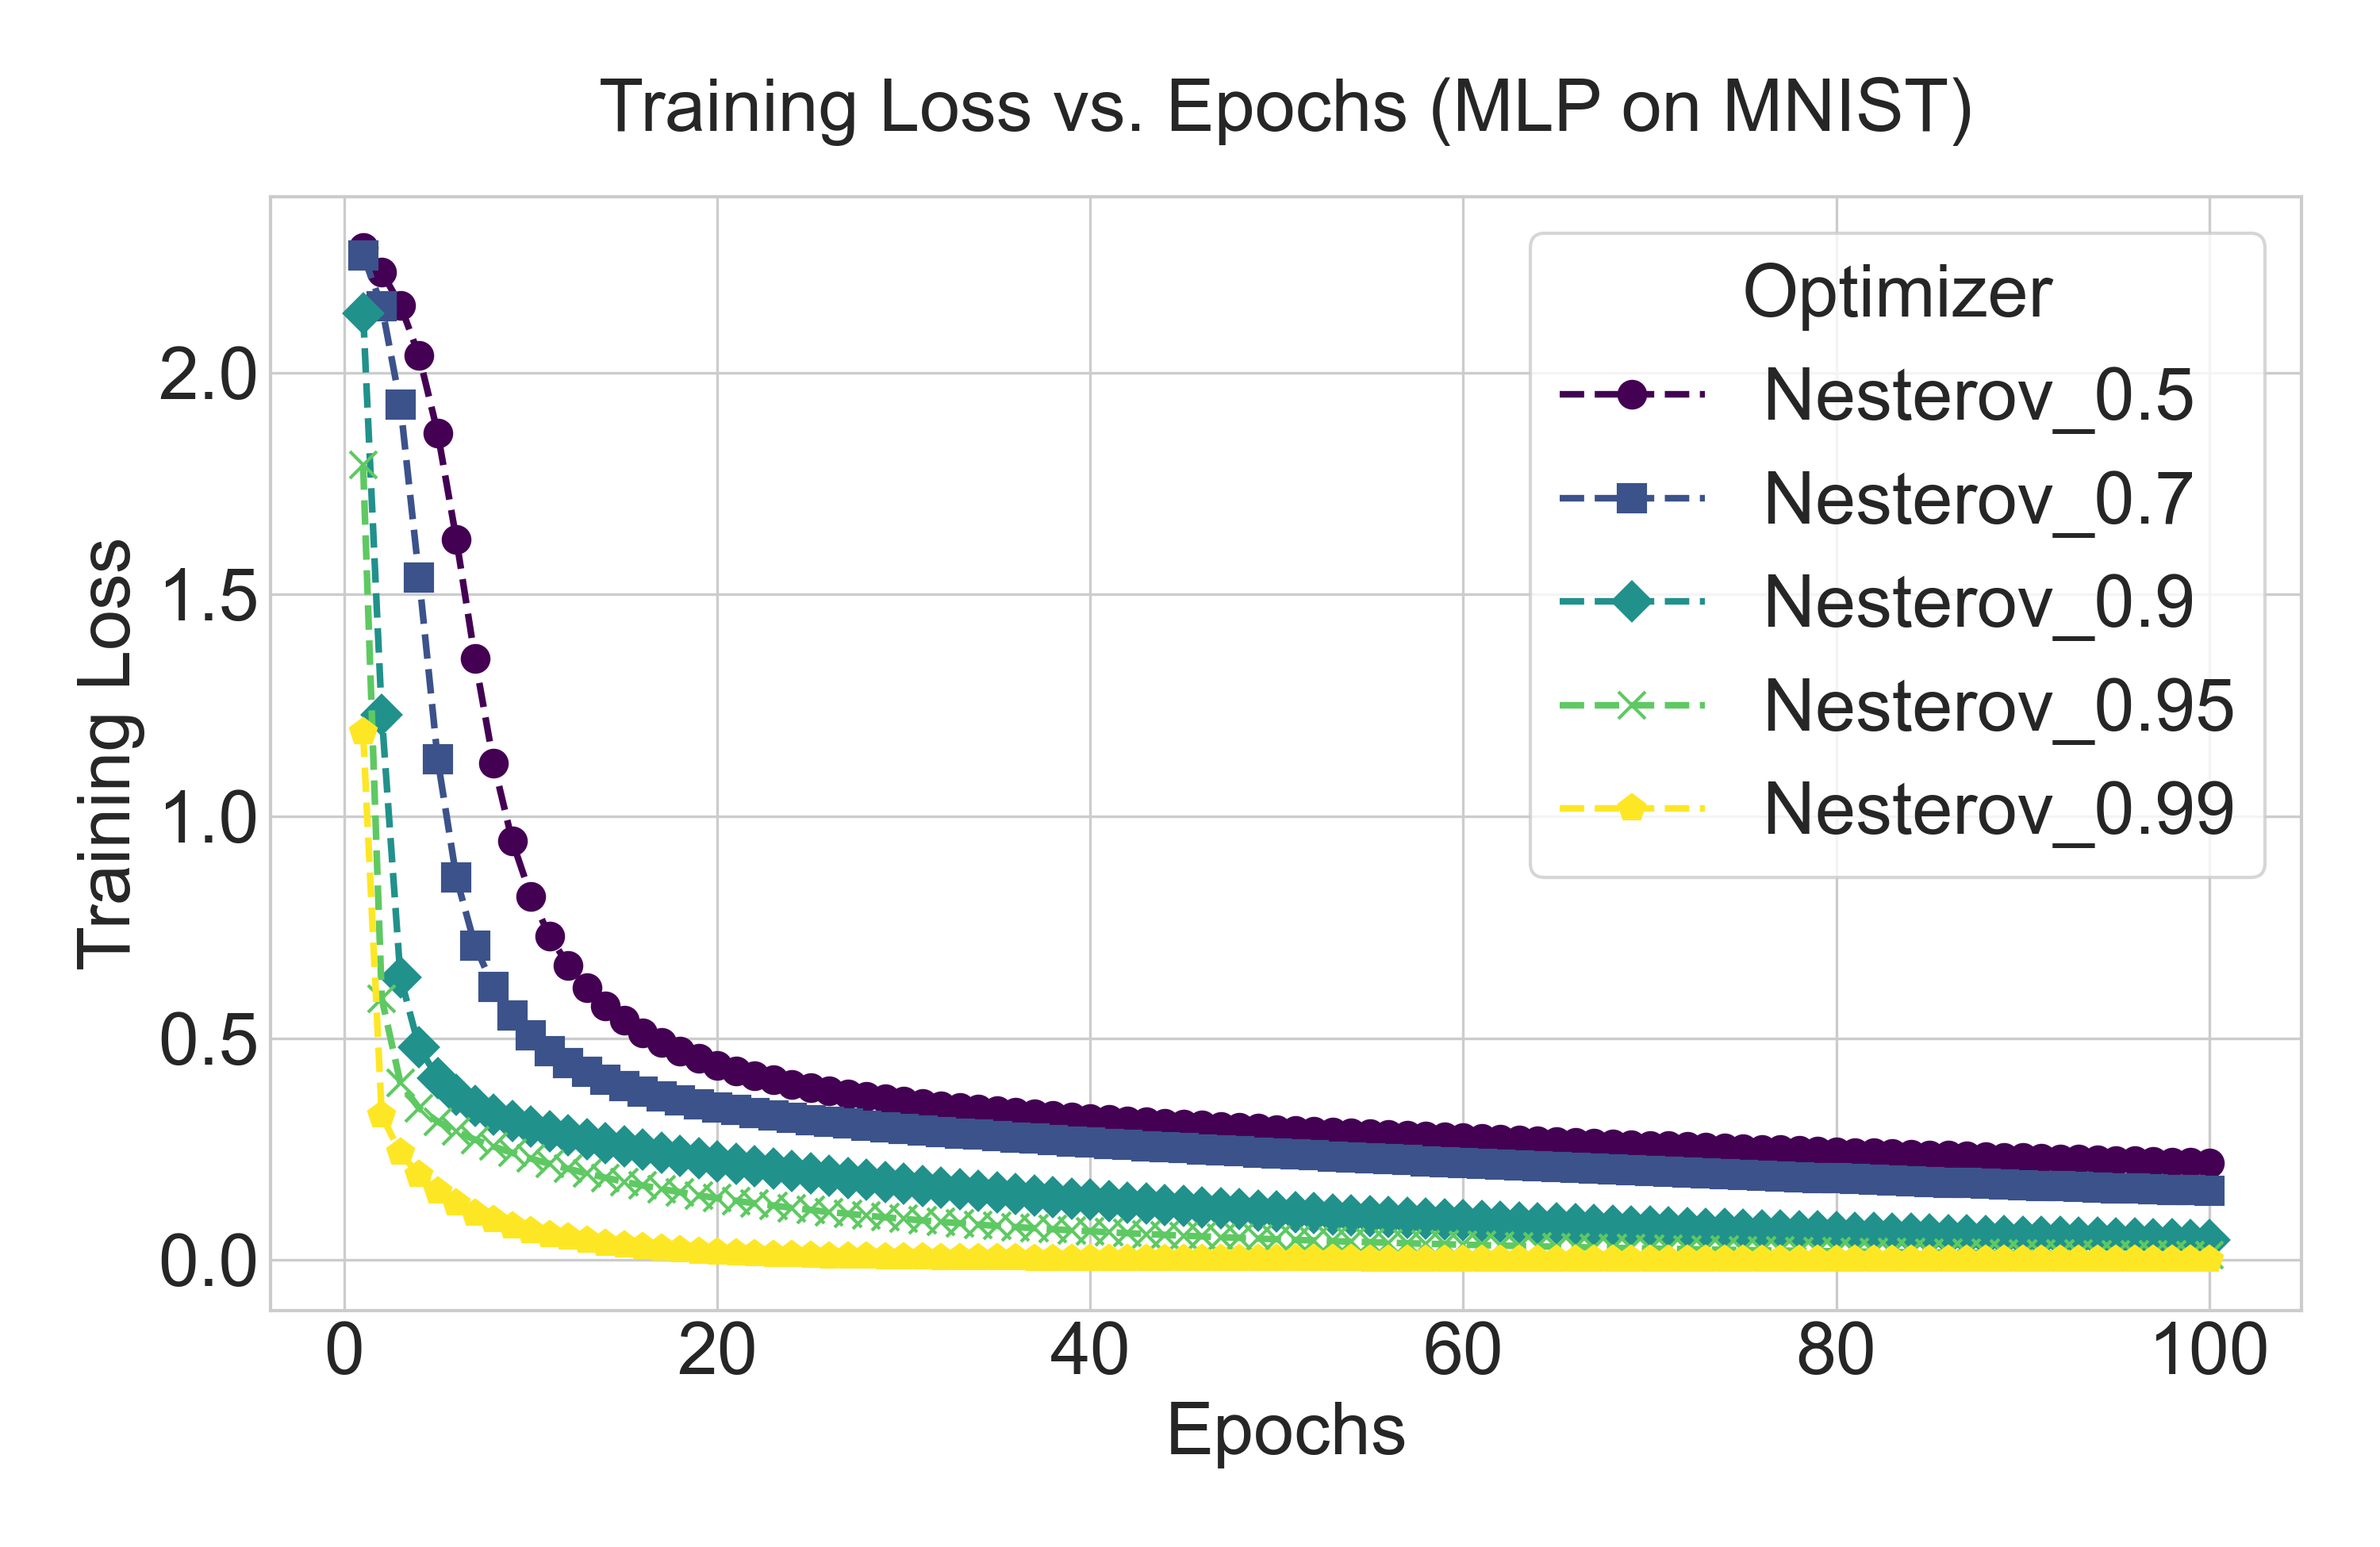
\includegraphics[width=0.48\textwidth]{Analysis_6_Nesterov_Momentum1_mnist_mlp_training_loss.png}} \quad
    \subfloat[MLP Accuracy on MNIST]{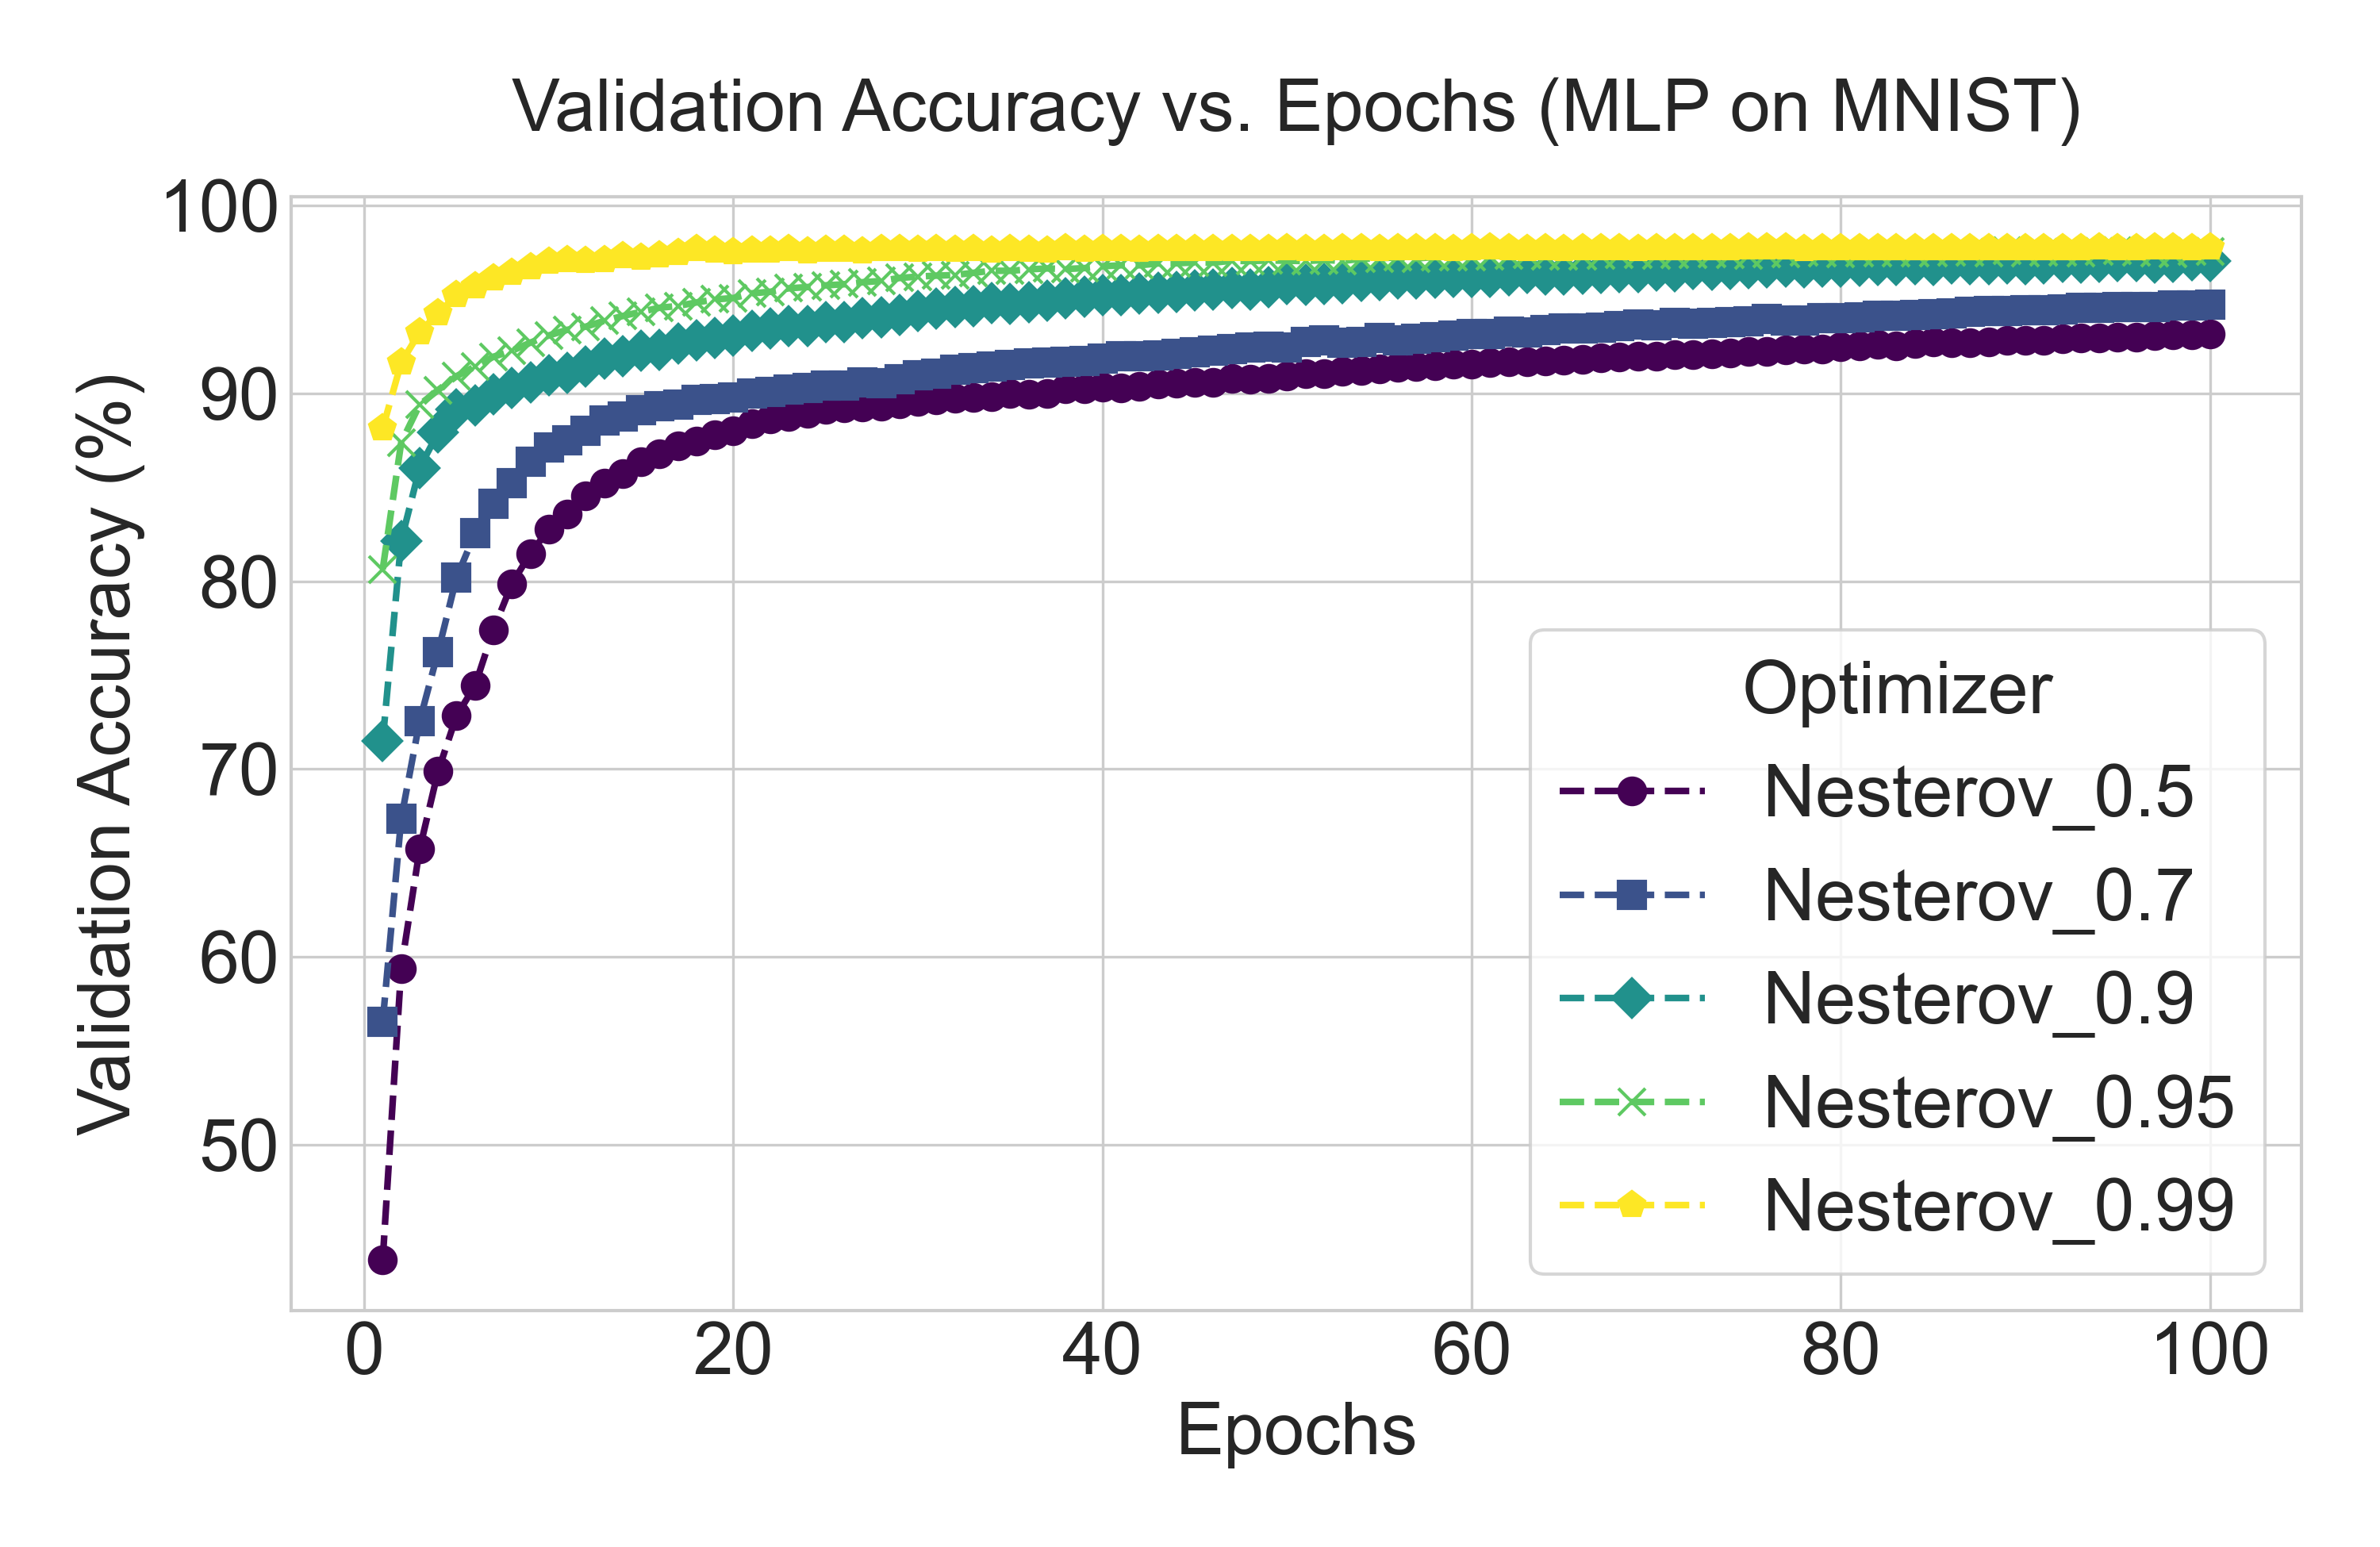
\includegraphics[width=0.48\textwidth]{Analysis_6_Nesterov_Momentum1_mnist_mlp_validation_accuracy.png}} \\
    % CNN row
    \subfloat[CNN Loss on CIFAR-10]{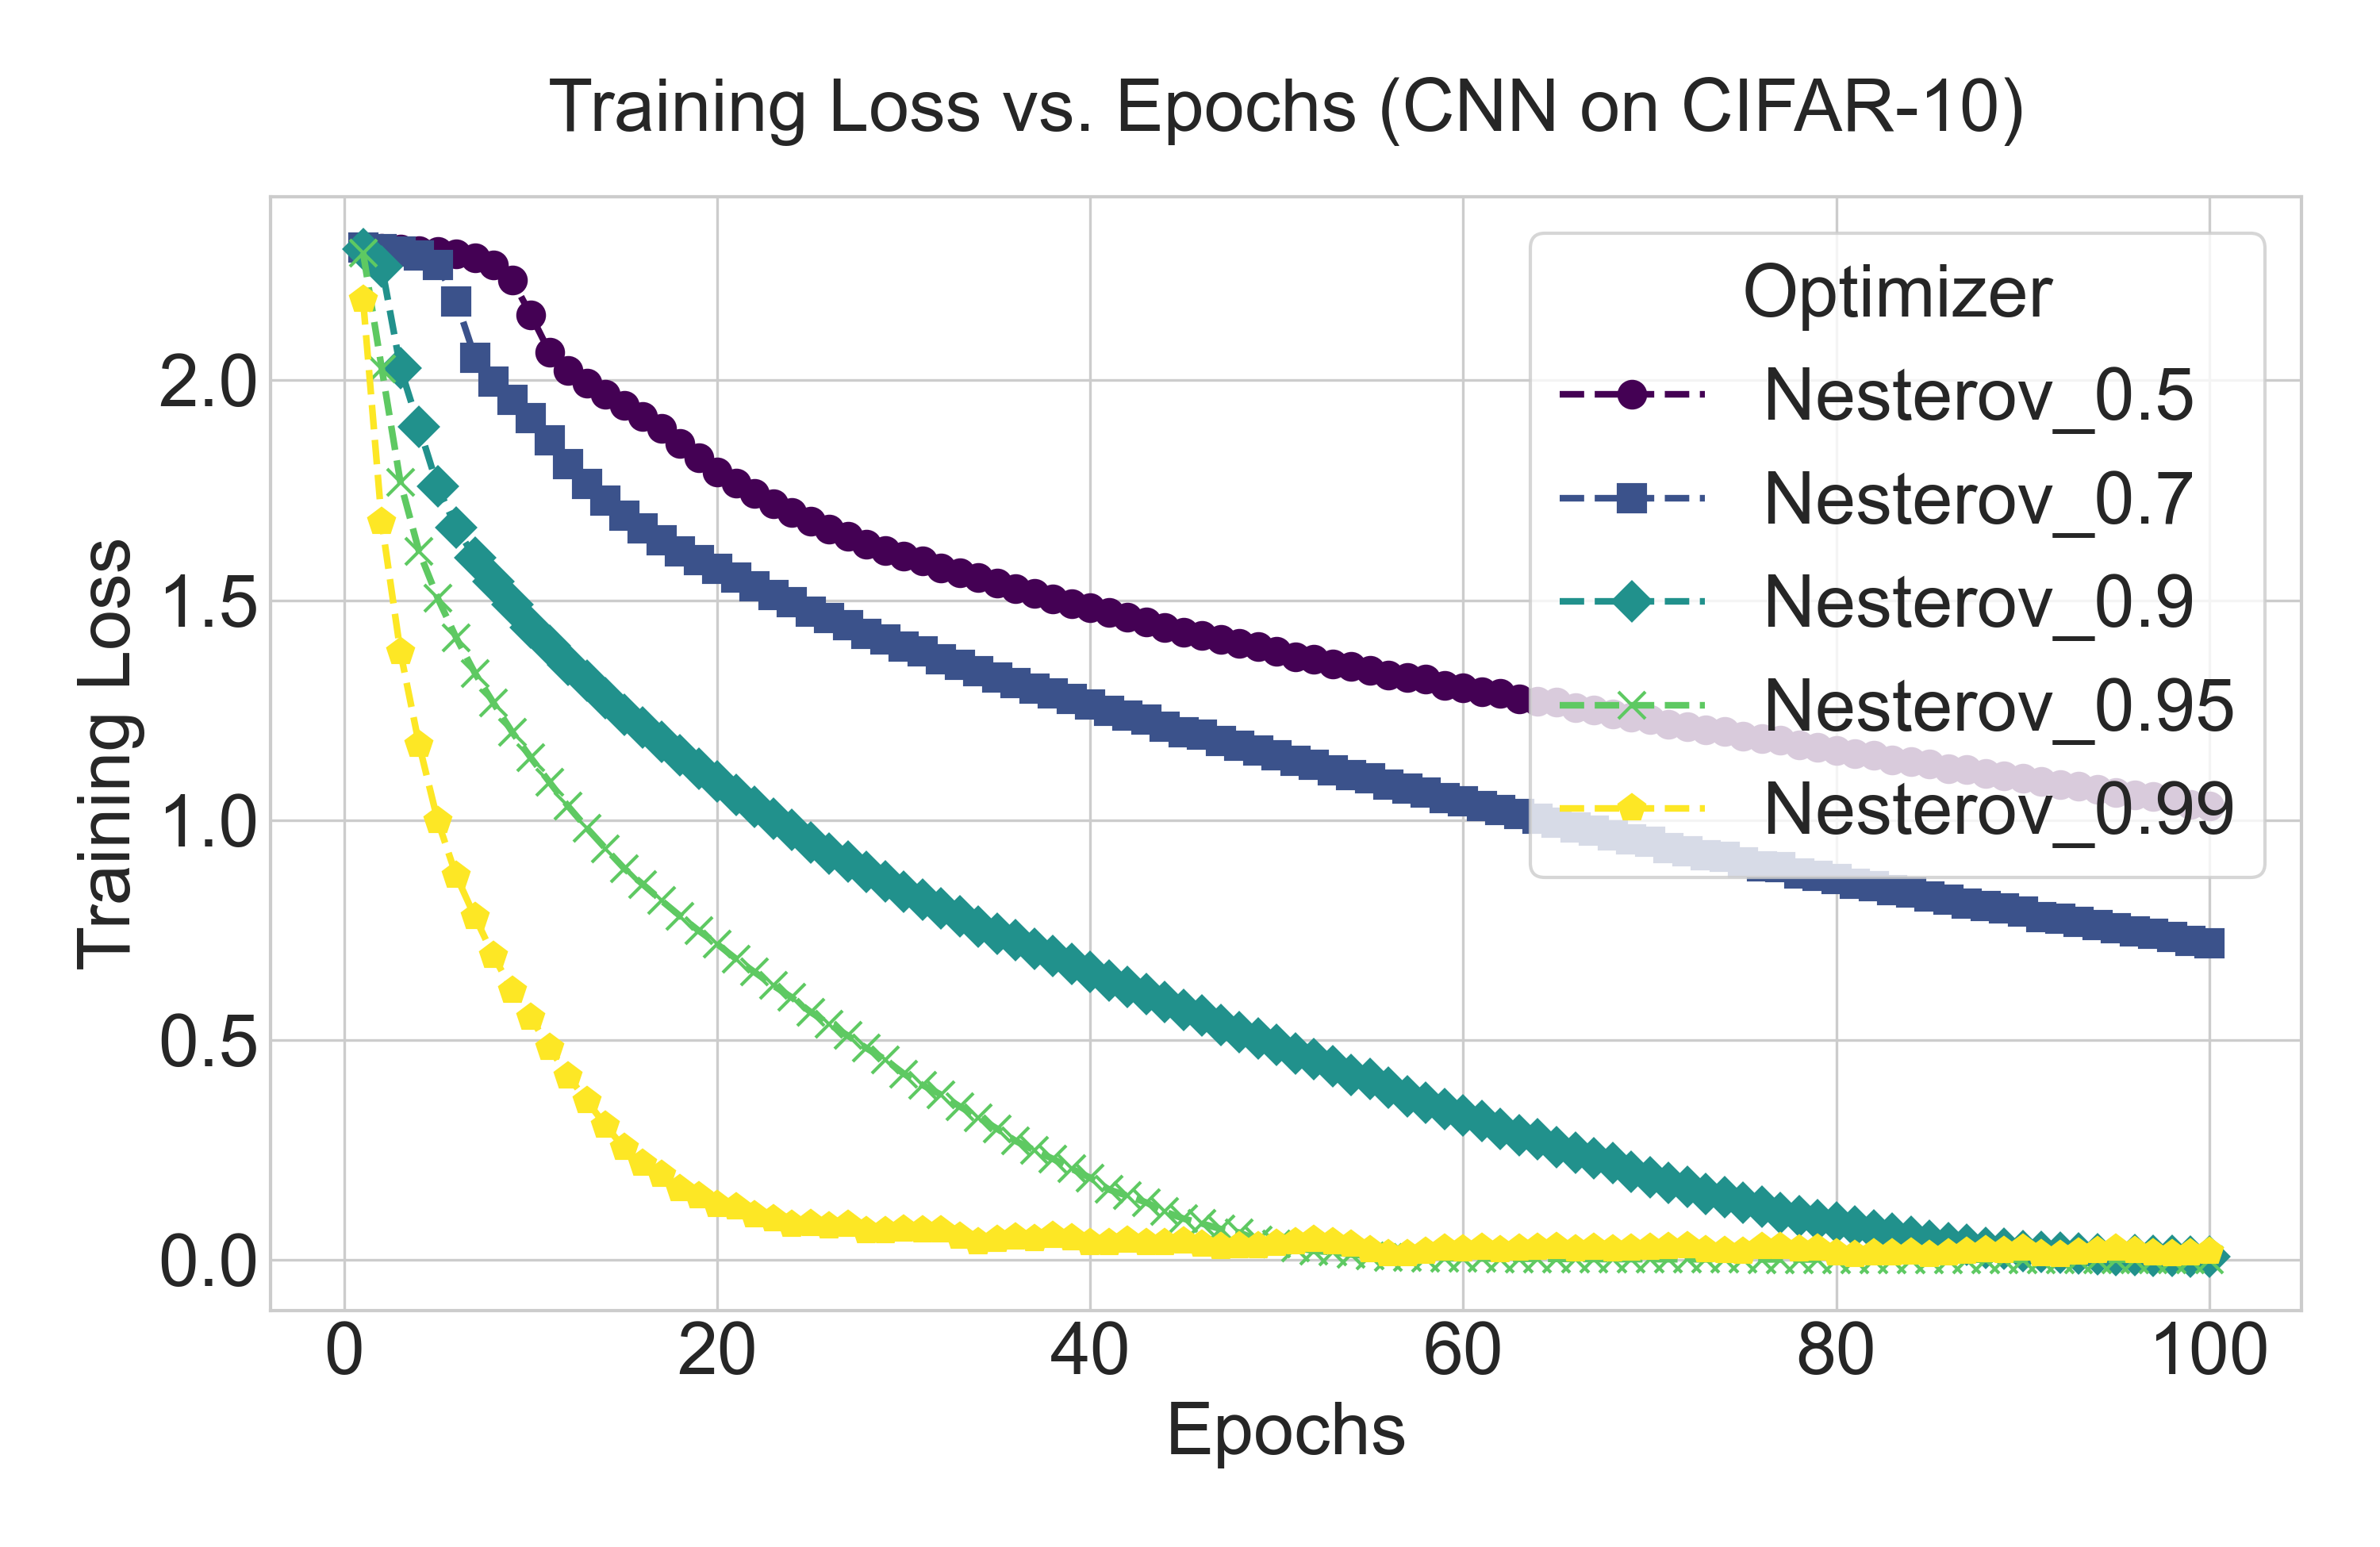
\includegraphics[width=0.48\textwidth]{Analysis_6_Nesterov_Momentum2_cifar10_cnn_training_loss.png}} \quad
    \subfloat[CNN Accuracy on CIFAR-10]{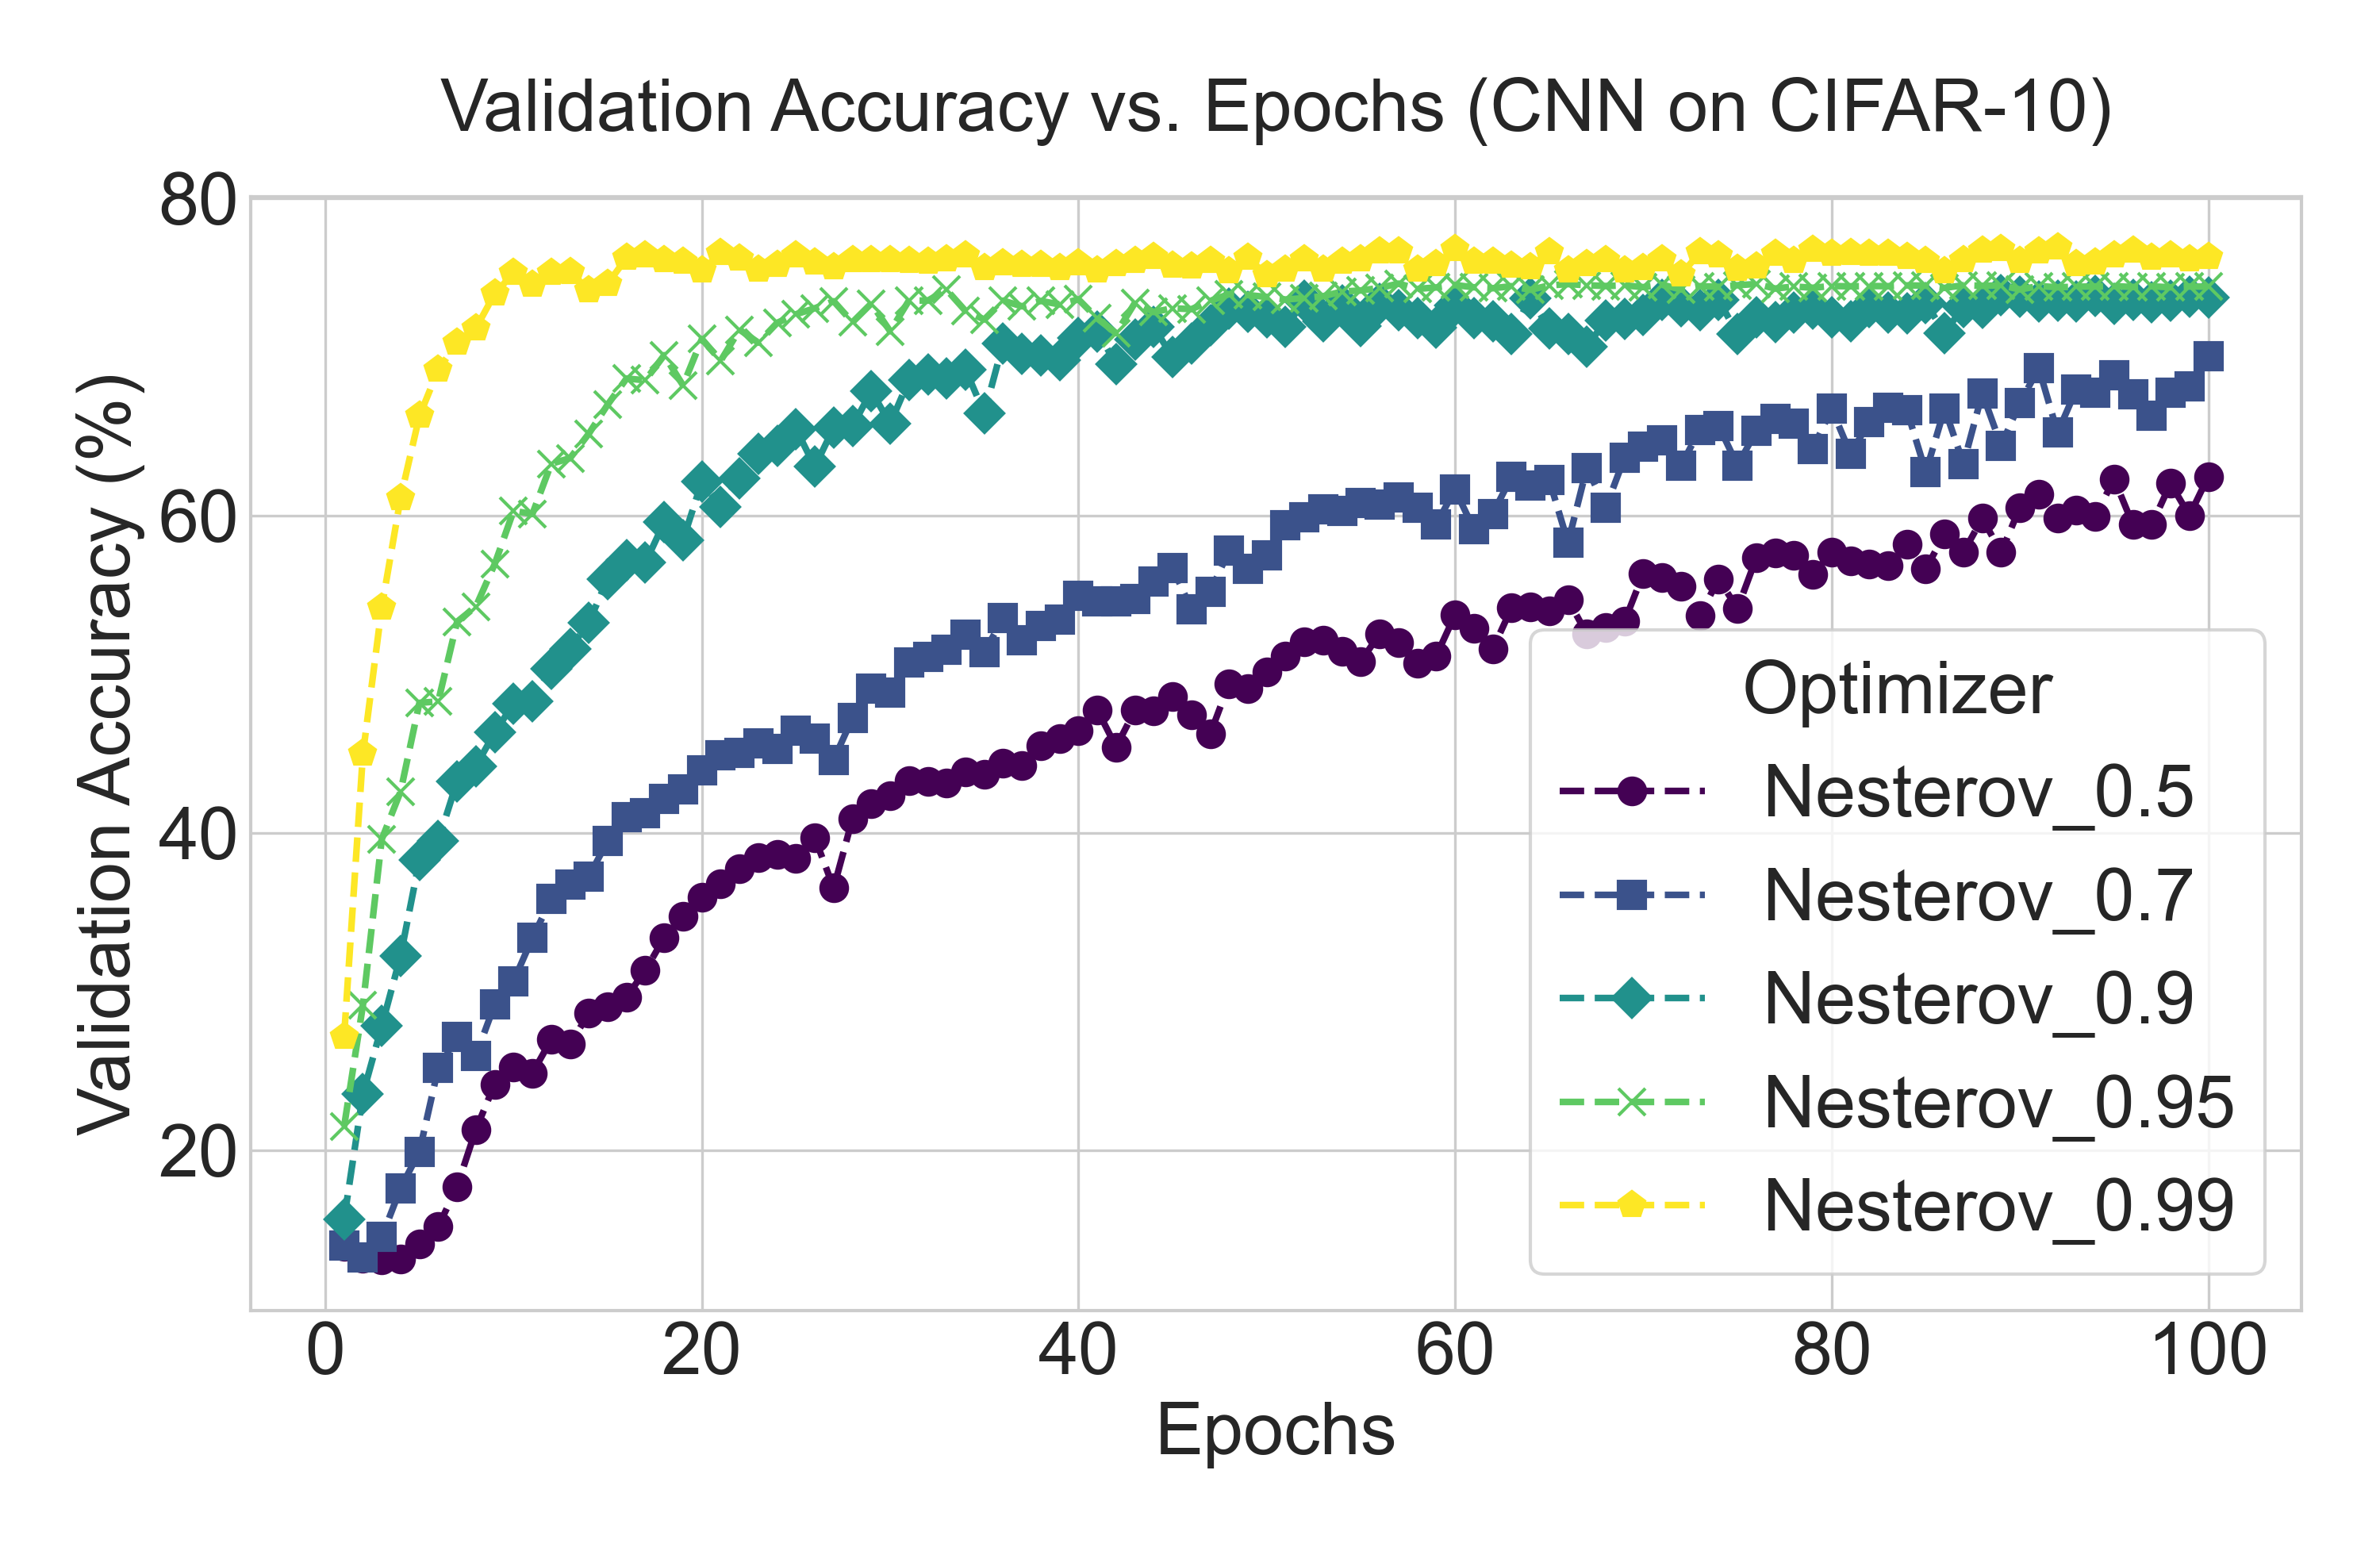
\includegraphics[width=0.48\textwidth]{Analysis_6_Nesterov_Momentum2_cifar10_cnn_validation_accuracy.png}} \\
    % VGG13 row
    \subfloat[VGG13 Loss on CIFAR-10]{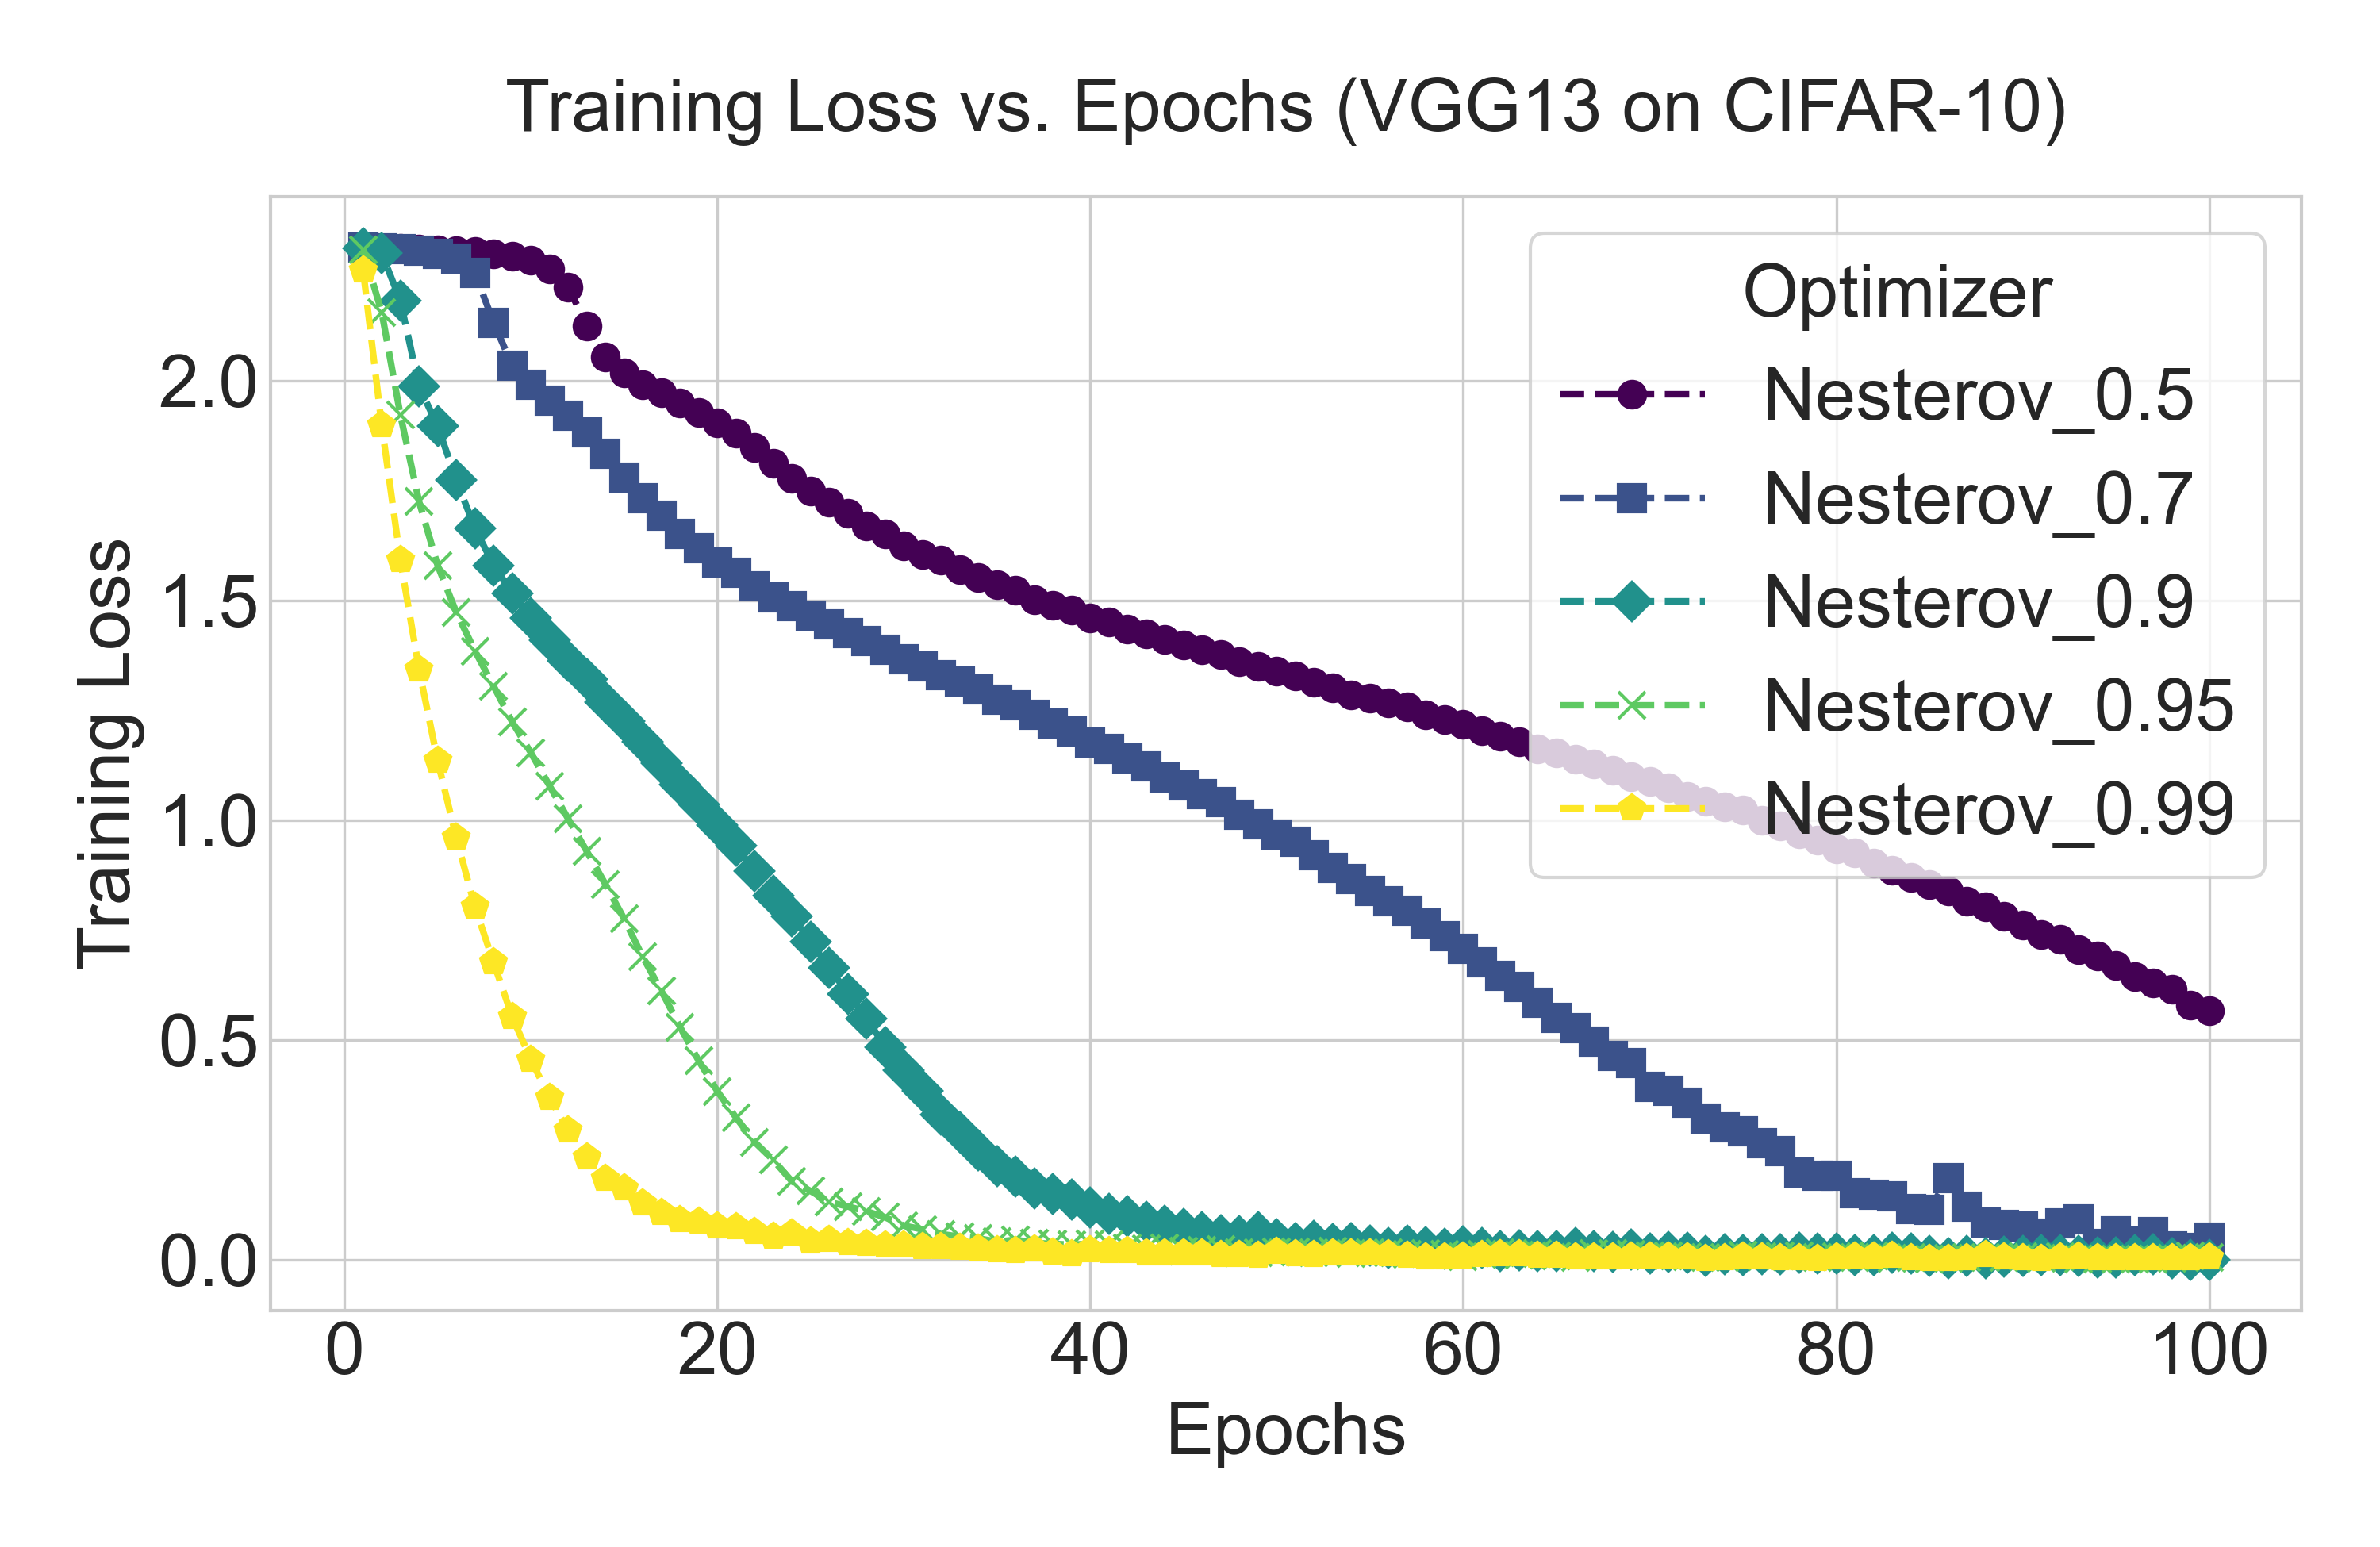
\includegraphics[width=0.48\textwidth]{Analysis_6_Nesterov_Momentum3_cifar_vgg13_training_loss.png}} \quad
    \subfloat[VGG13 Accuracy on CIFAR-10]{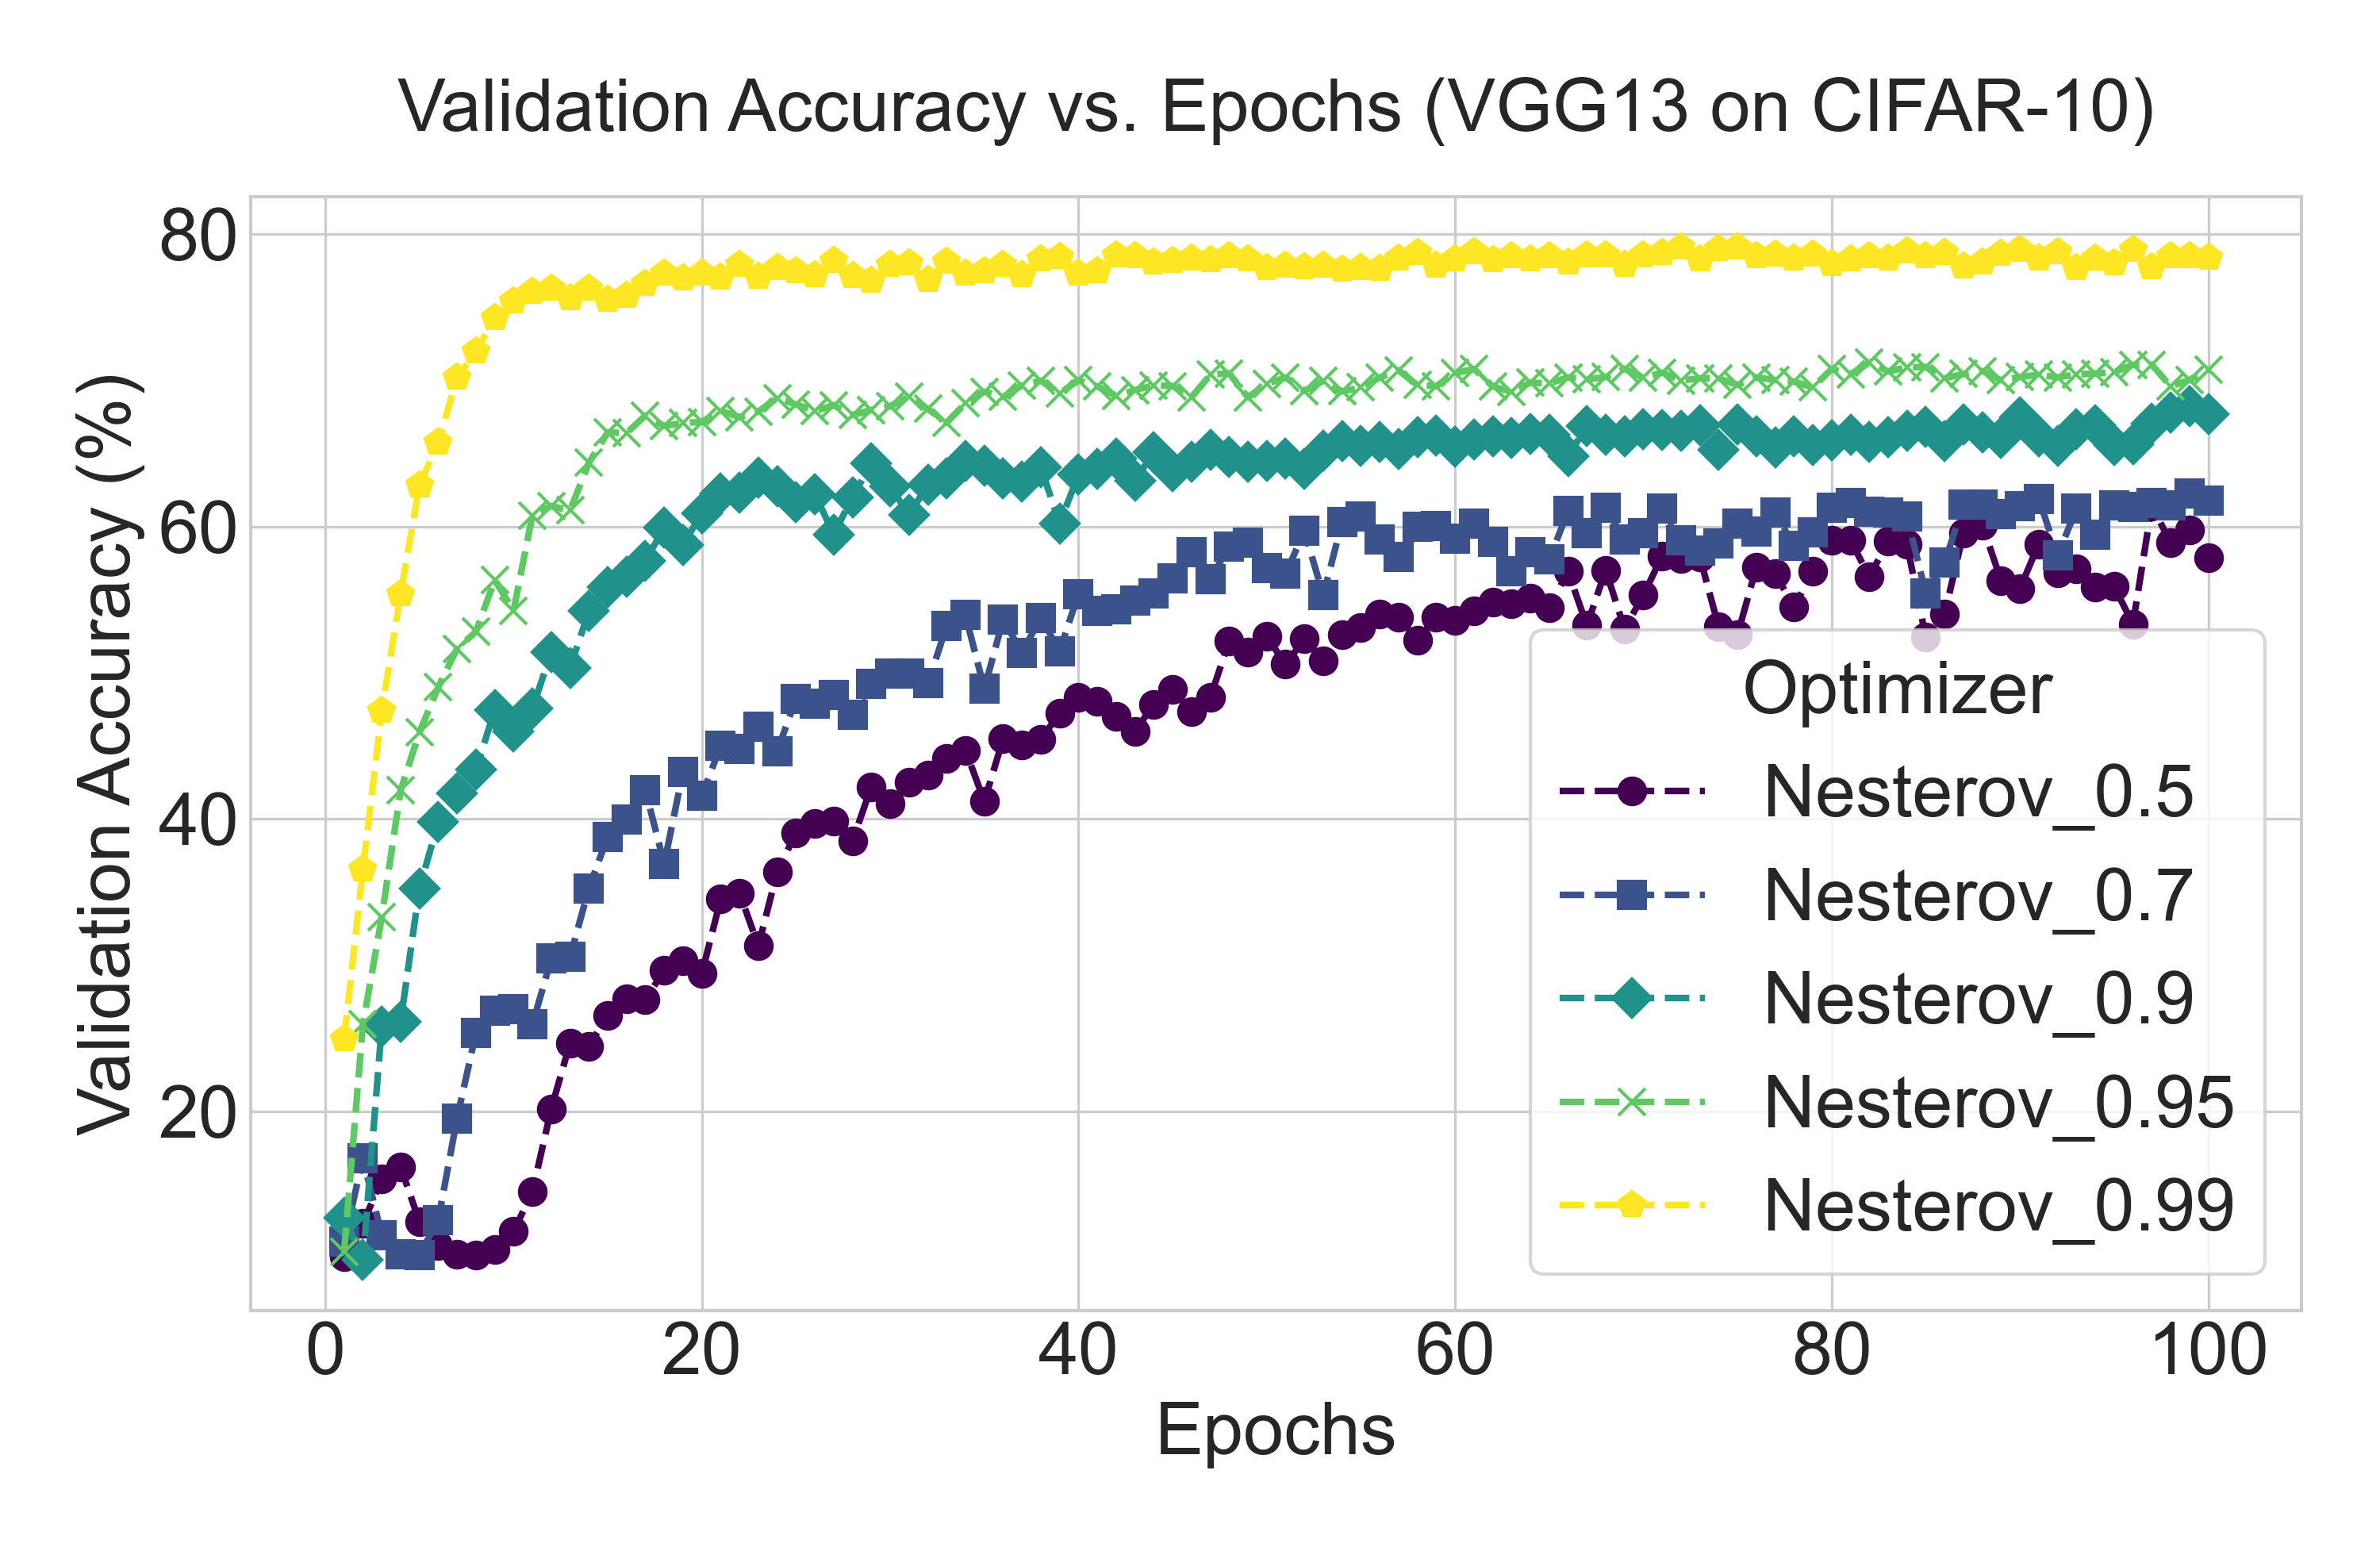
\includegraphics[width=0.48\textwidth]{Analysis_6_Nesterov_Momentum3_cifar_vgg13_validation_accuracy.png}}
    \caption{Impact of Nesterov momentum: baseline method (Polyak momentum, purple line) vs. Nesterov momentum (orange line)}
    \label{fig:nesterov_momentum_study}
\end{figure}

%-------------------------
\clearpage
\subsection*{(b) Polyak Momentum}

\begin{figure}[htbp]
    \centering
    % MLP row
    \subfloat[MLP Loss on MNIST]{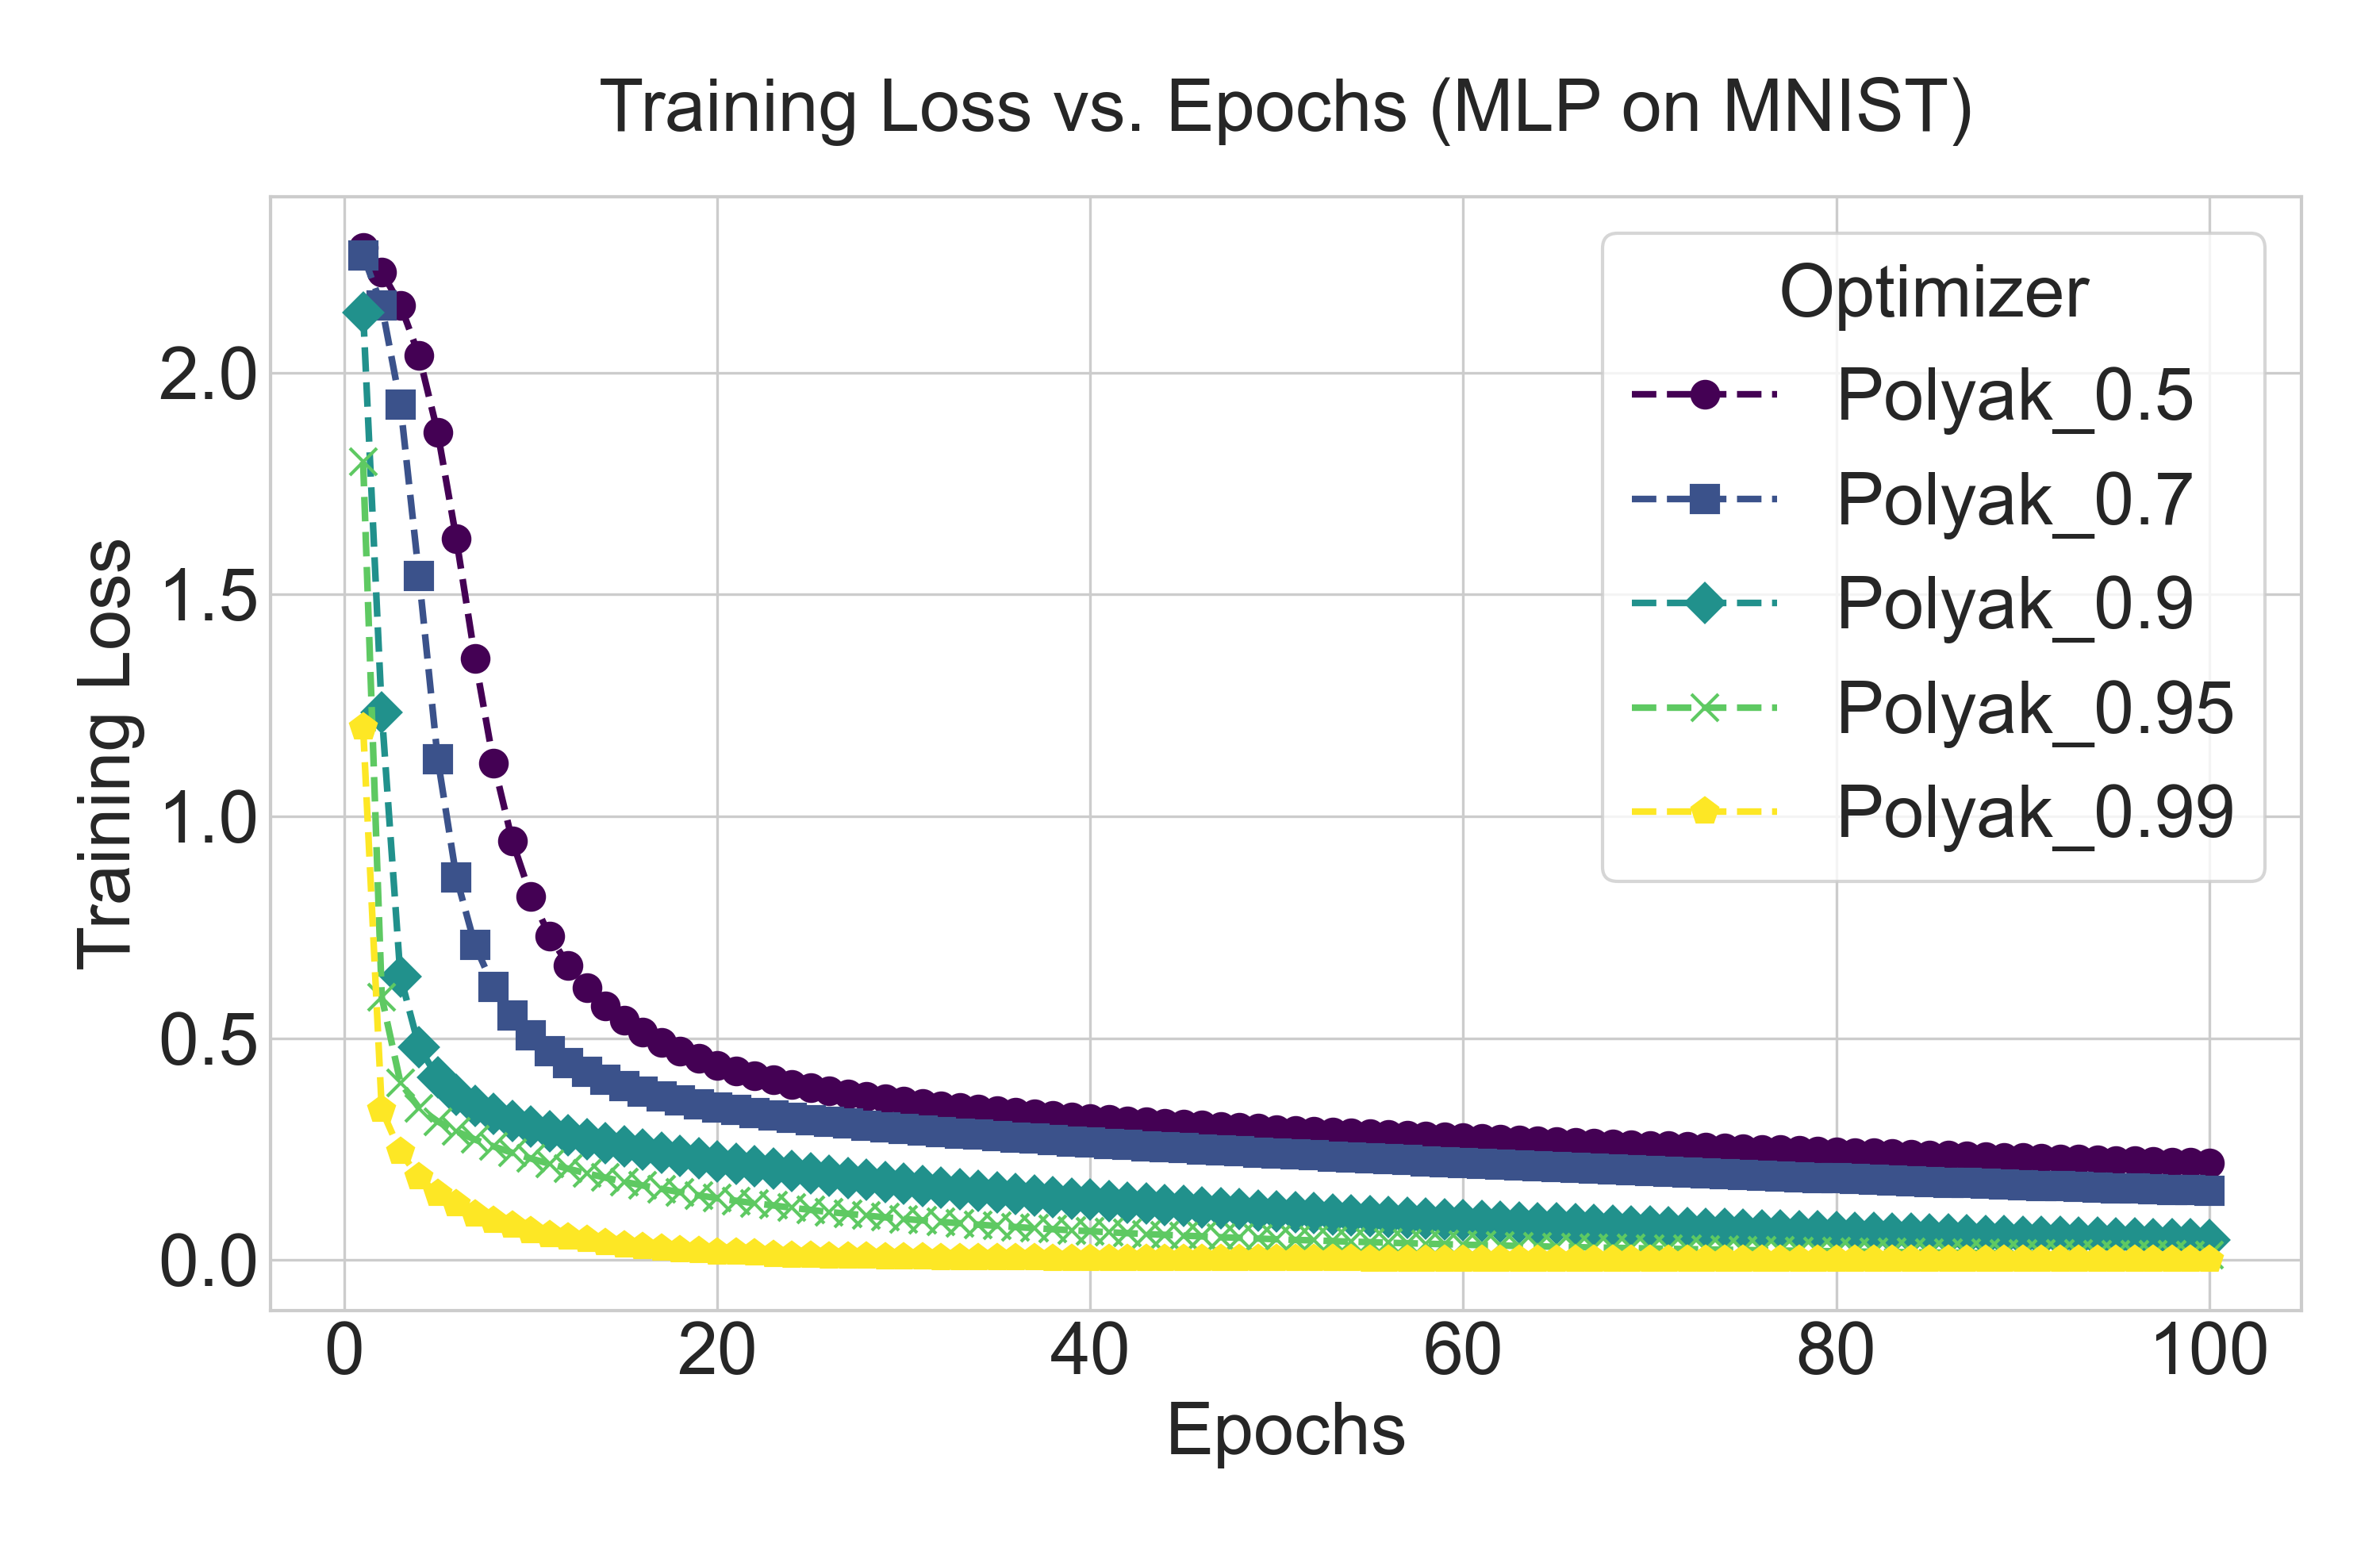
\includegraphics[width=0.48\textwidth]{Analysis_5_Polyak_Momentum1_mnist_mlp_training_loss.png}} \quad
    \subfloat[MLP Accuracy on MNIST]{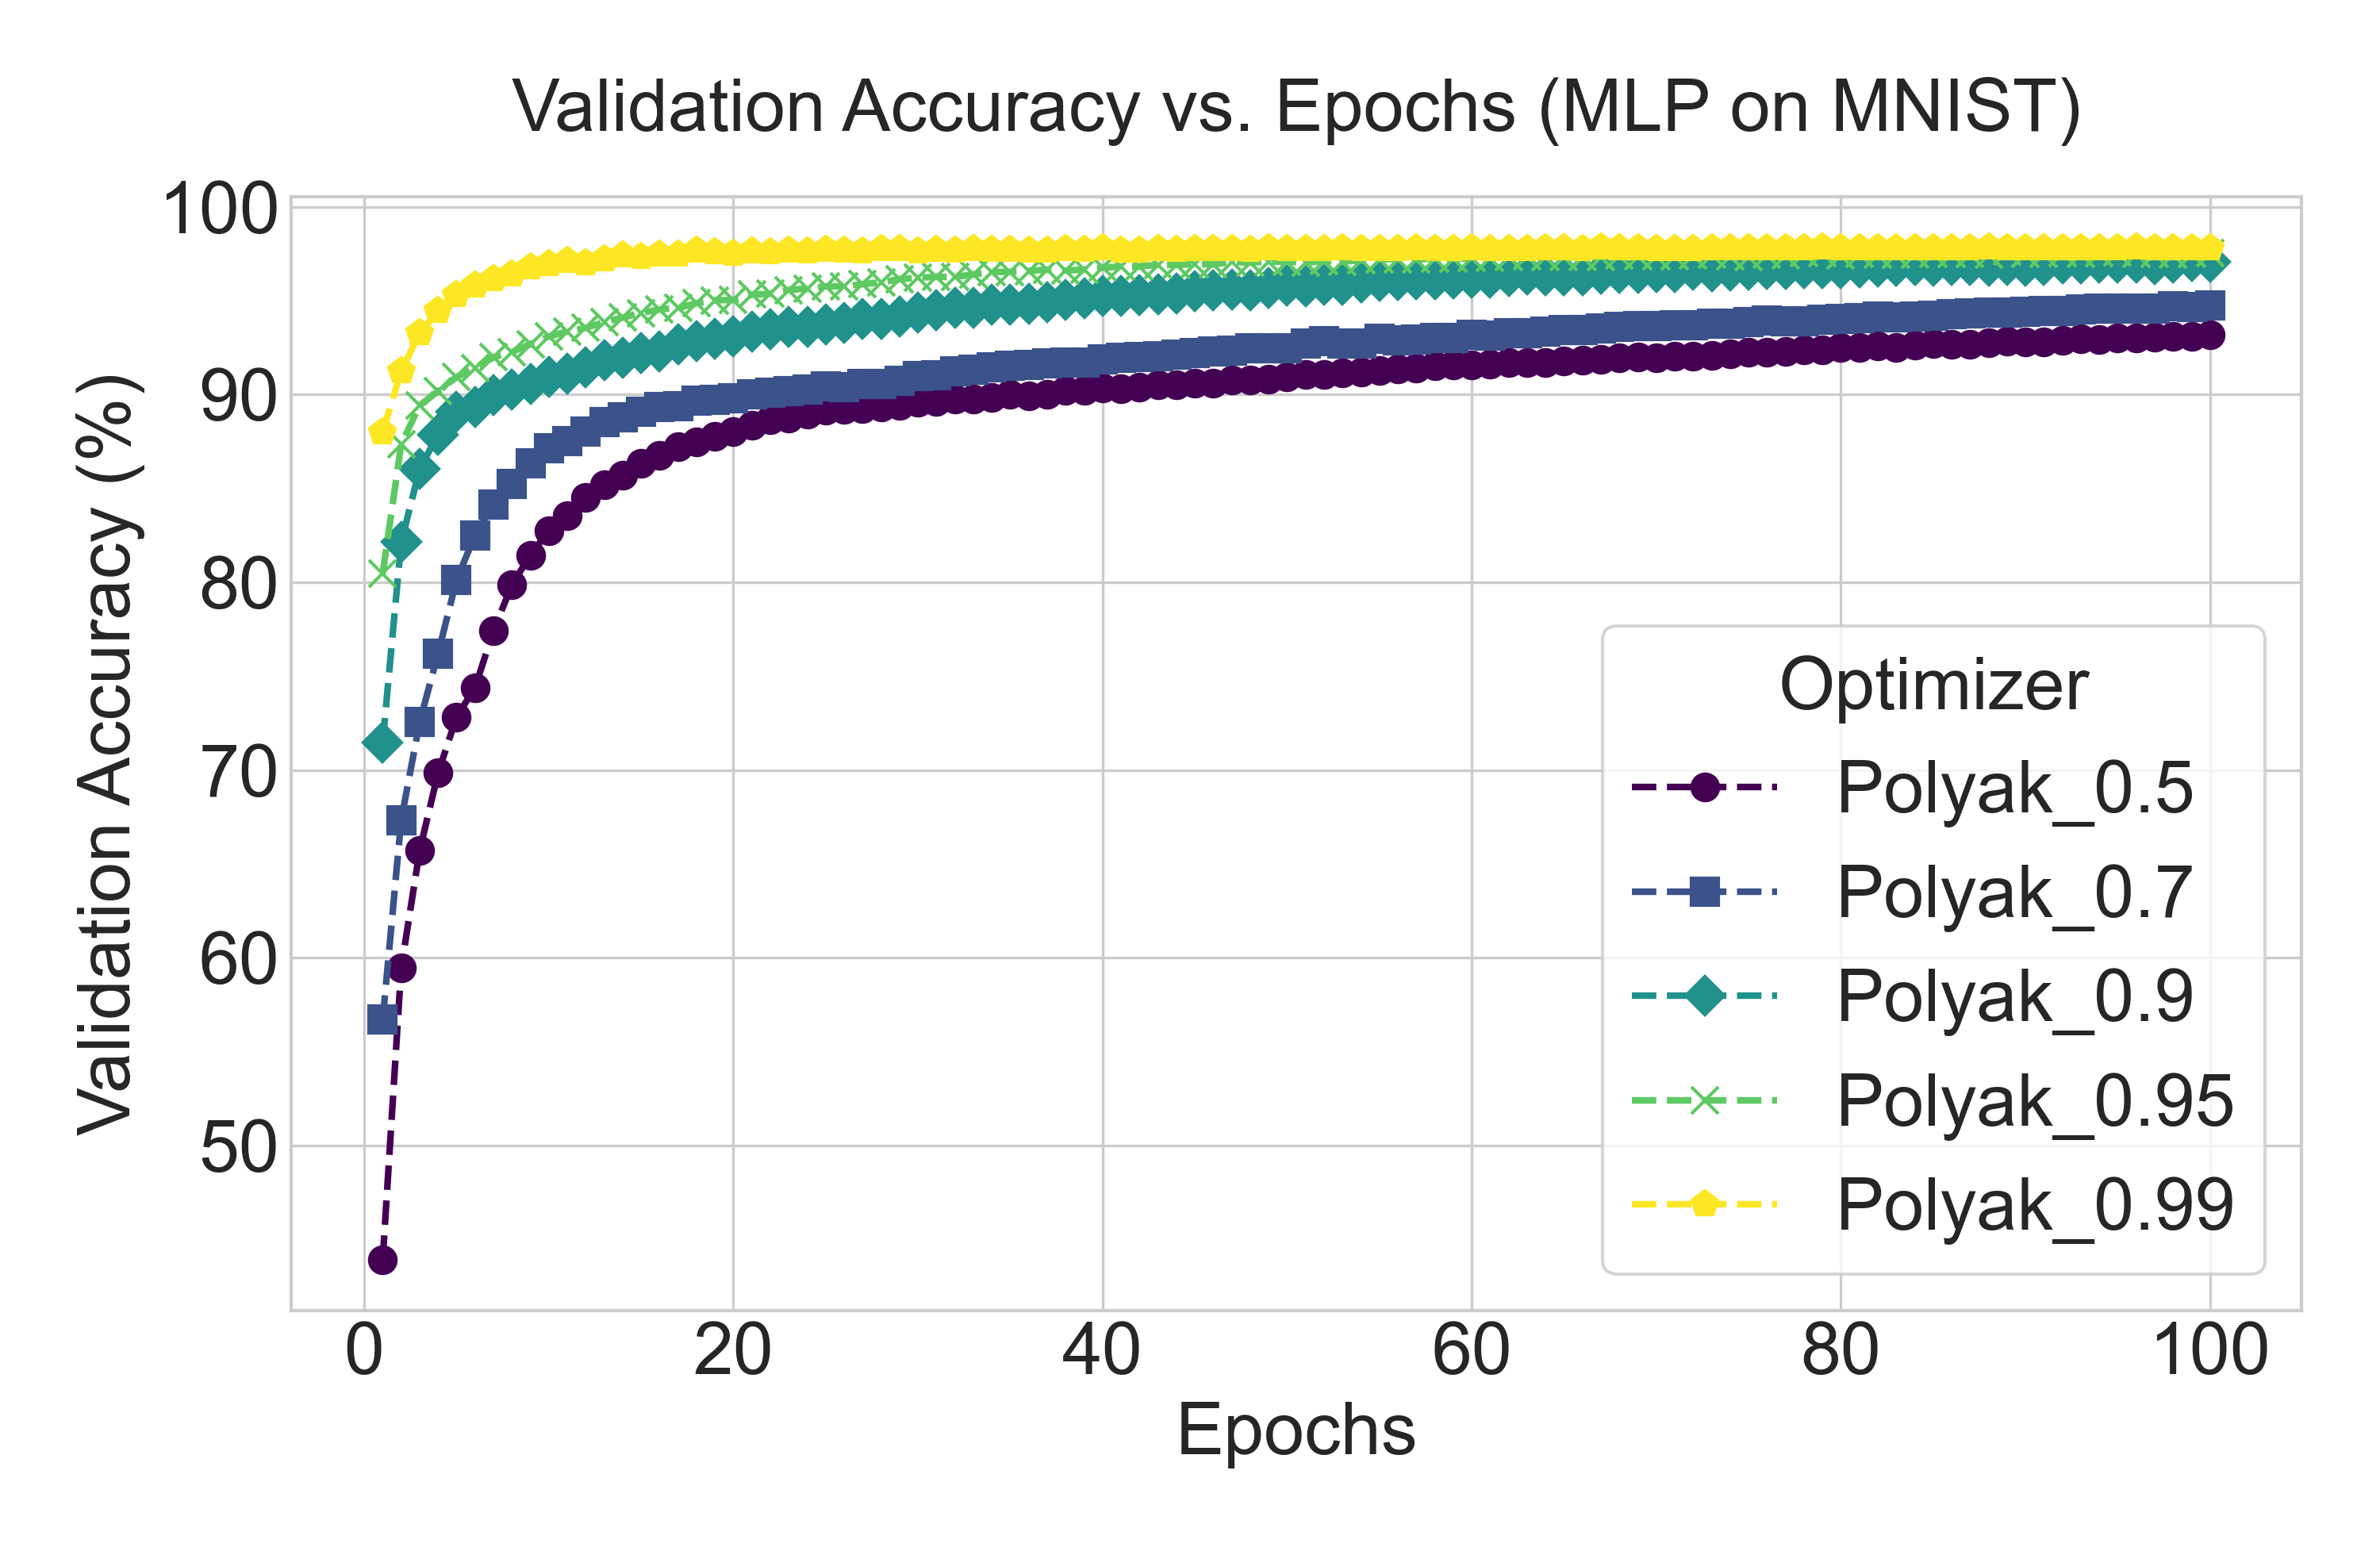
\includegraphics[width=0.48\textwidth]{Analysis_5_Polyak_Momentum1_mnist_mlp_validation_accuracy.png}} \\
    % CNN row
    \subfloat[CNN Loss on CIFAR-10]{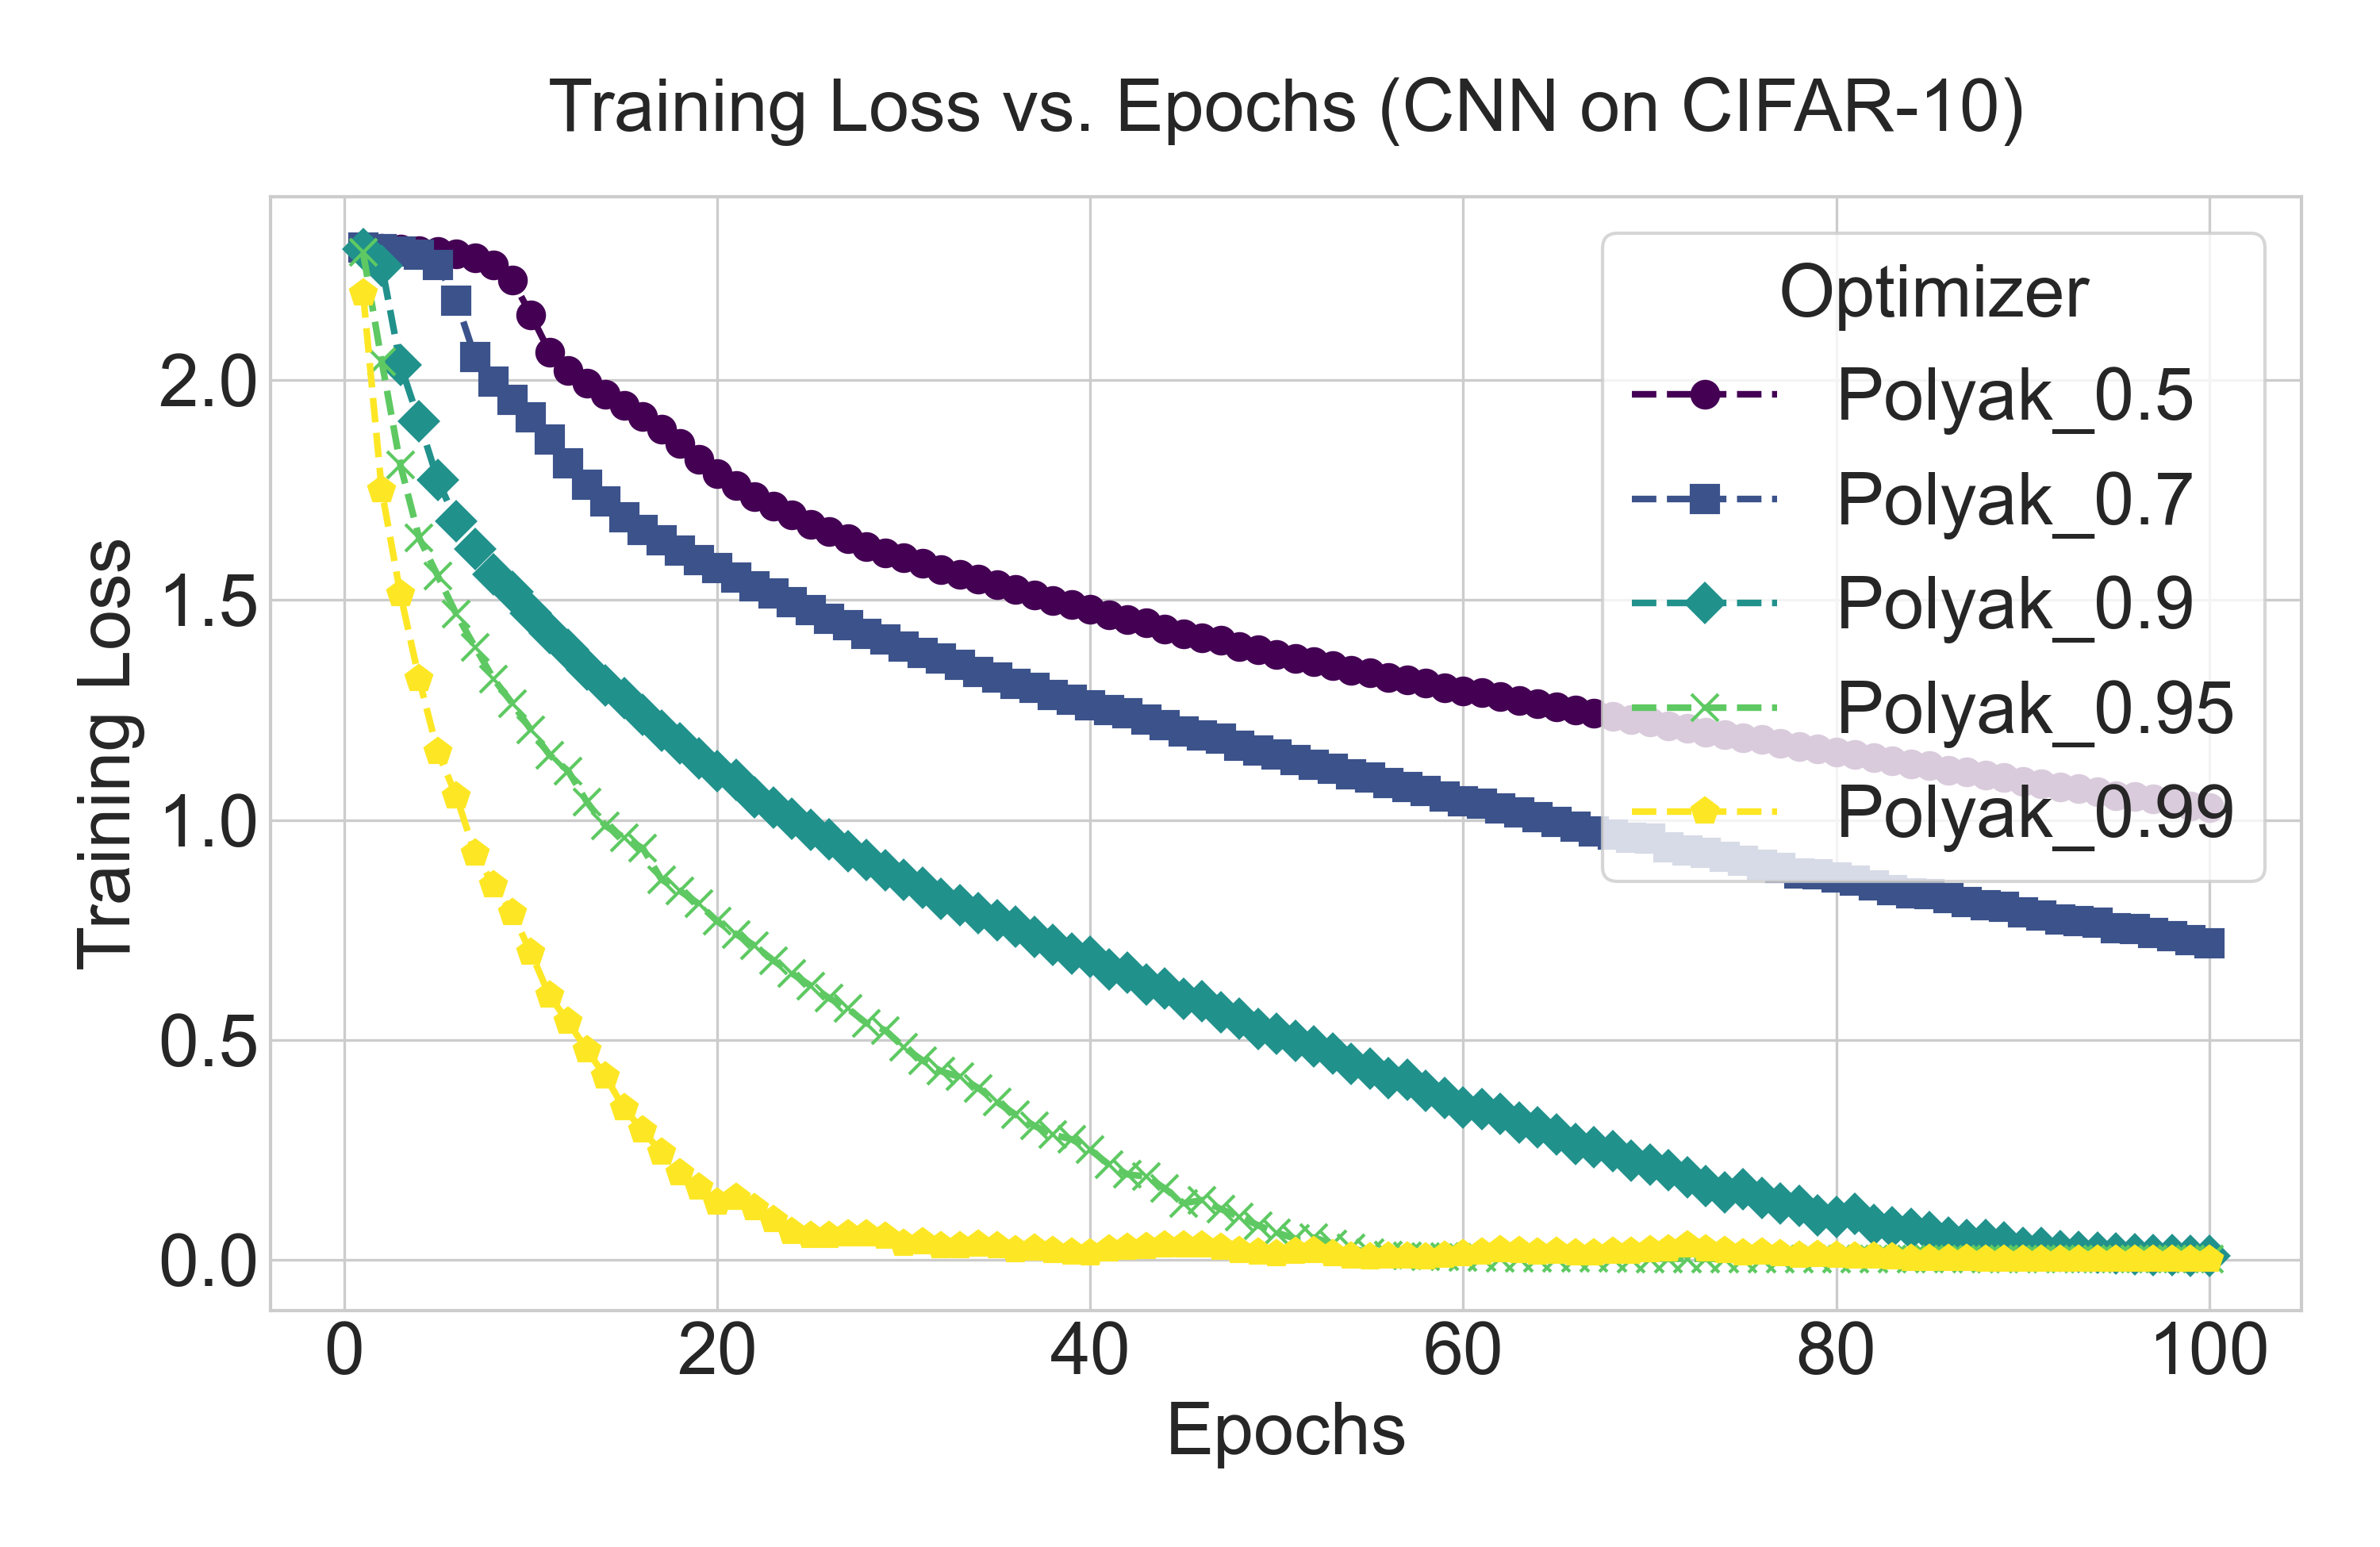
\includegraphics[width=0.48\textwidth]{Analysis_5_Polyak_Momentum2_cifar10_cnn_training_loss.png}} \quad
    \subfloat[CNN Accuracy on CIFAR-10]{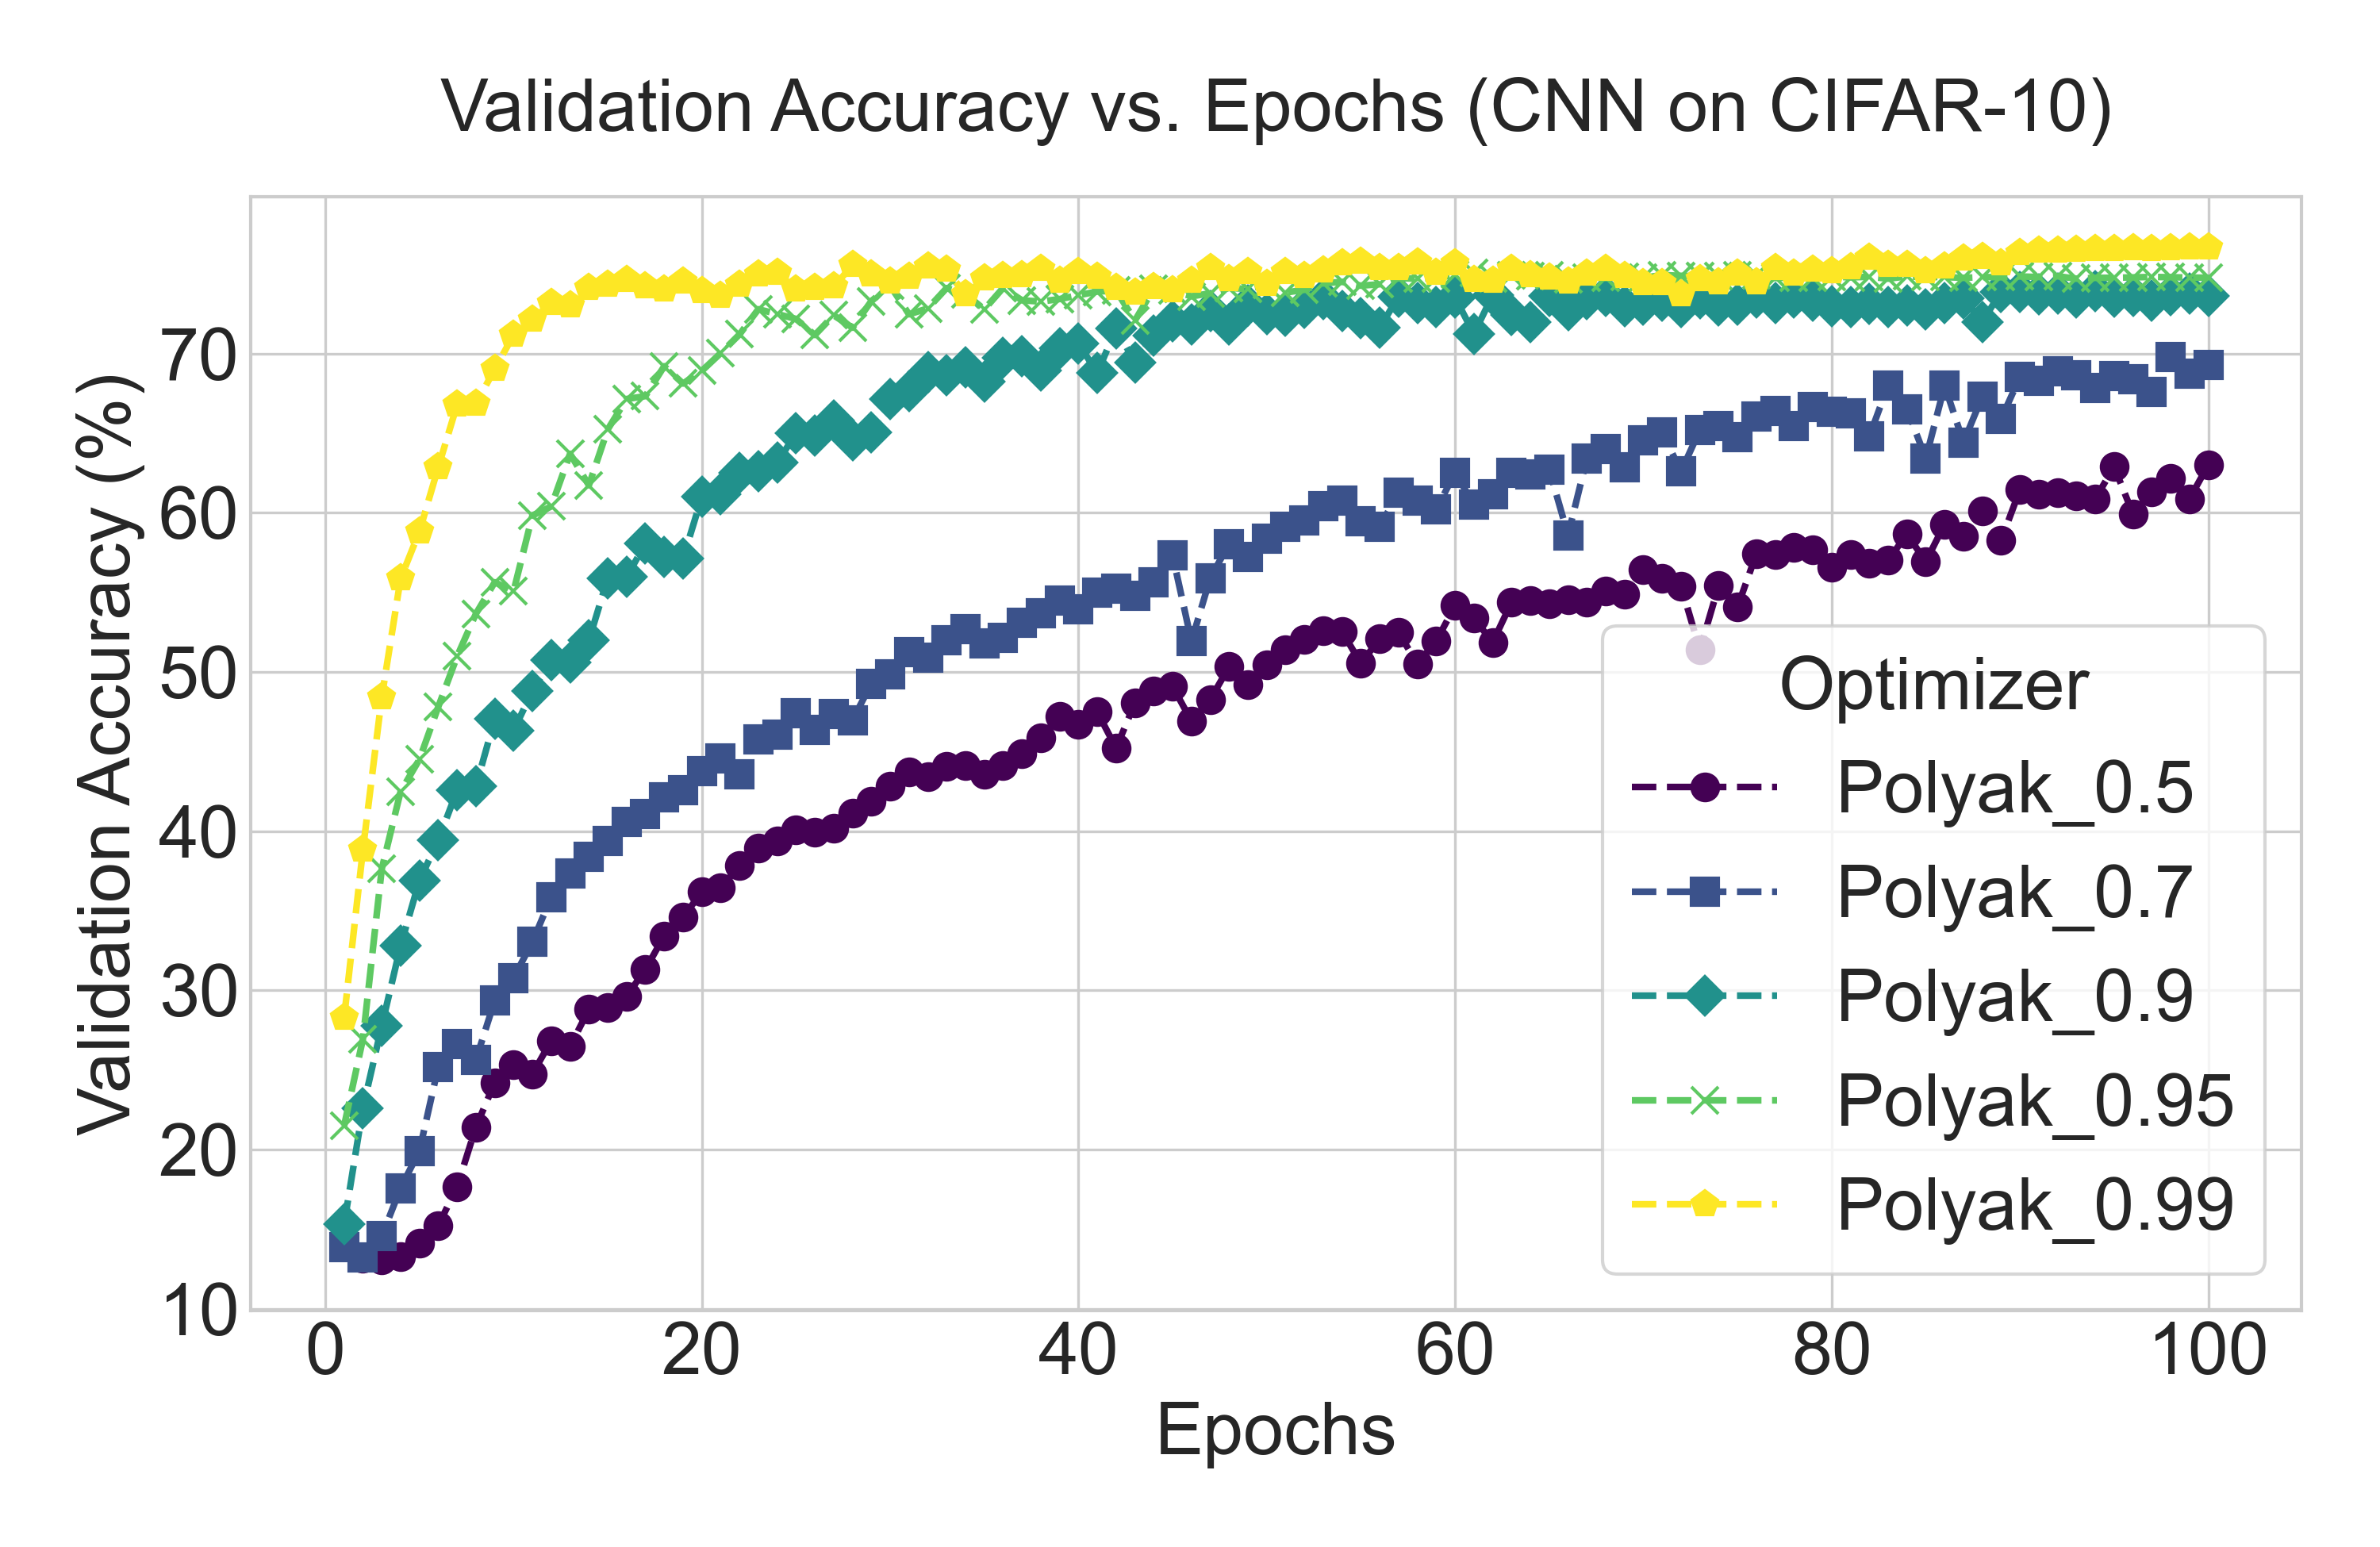
\includegraphics[width=0.48\textwidth]{Analysis_5_Polyak_Momentum2_cifar10_cnn_validation_accuracy.png}} \\
    % VGG13 row
    \subfloat[VGG13 Loss on CIFAR-10]{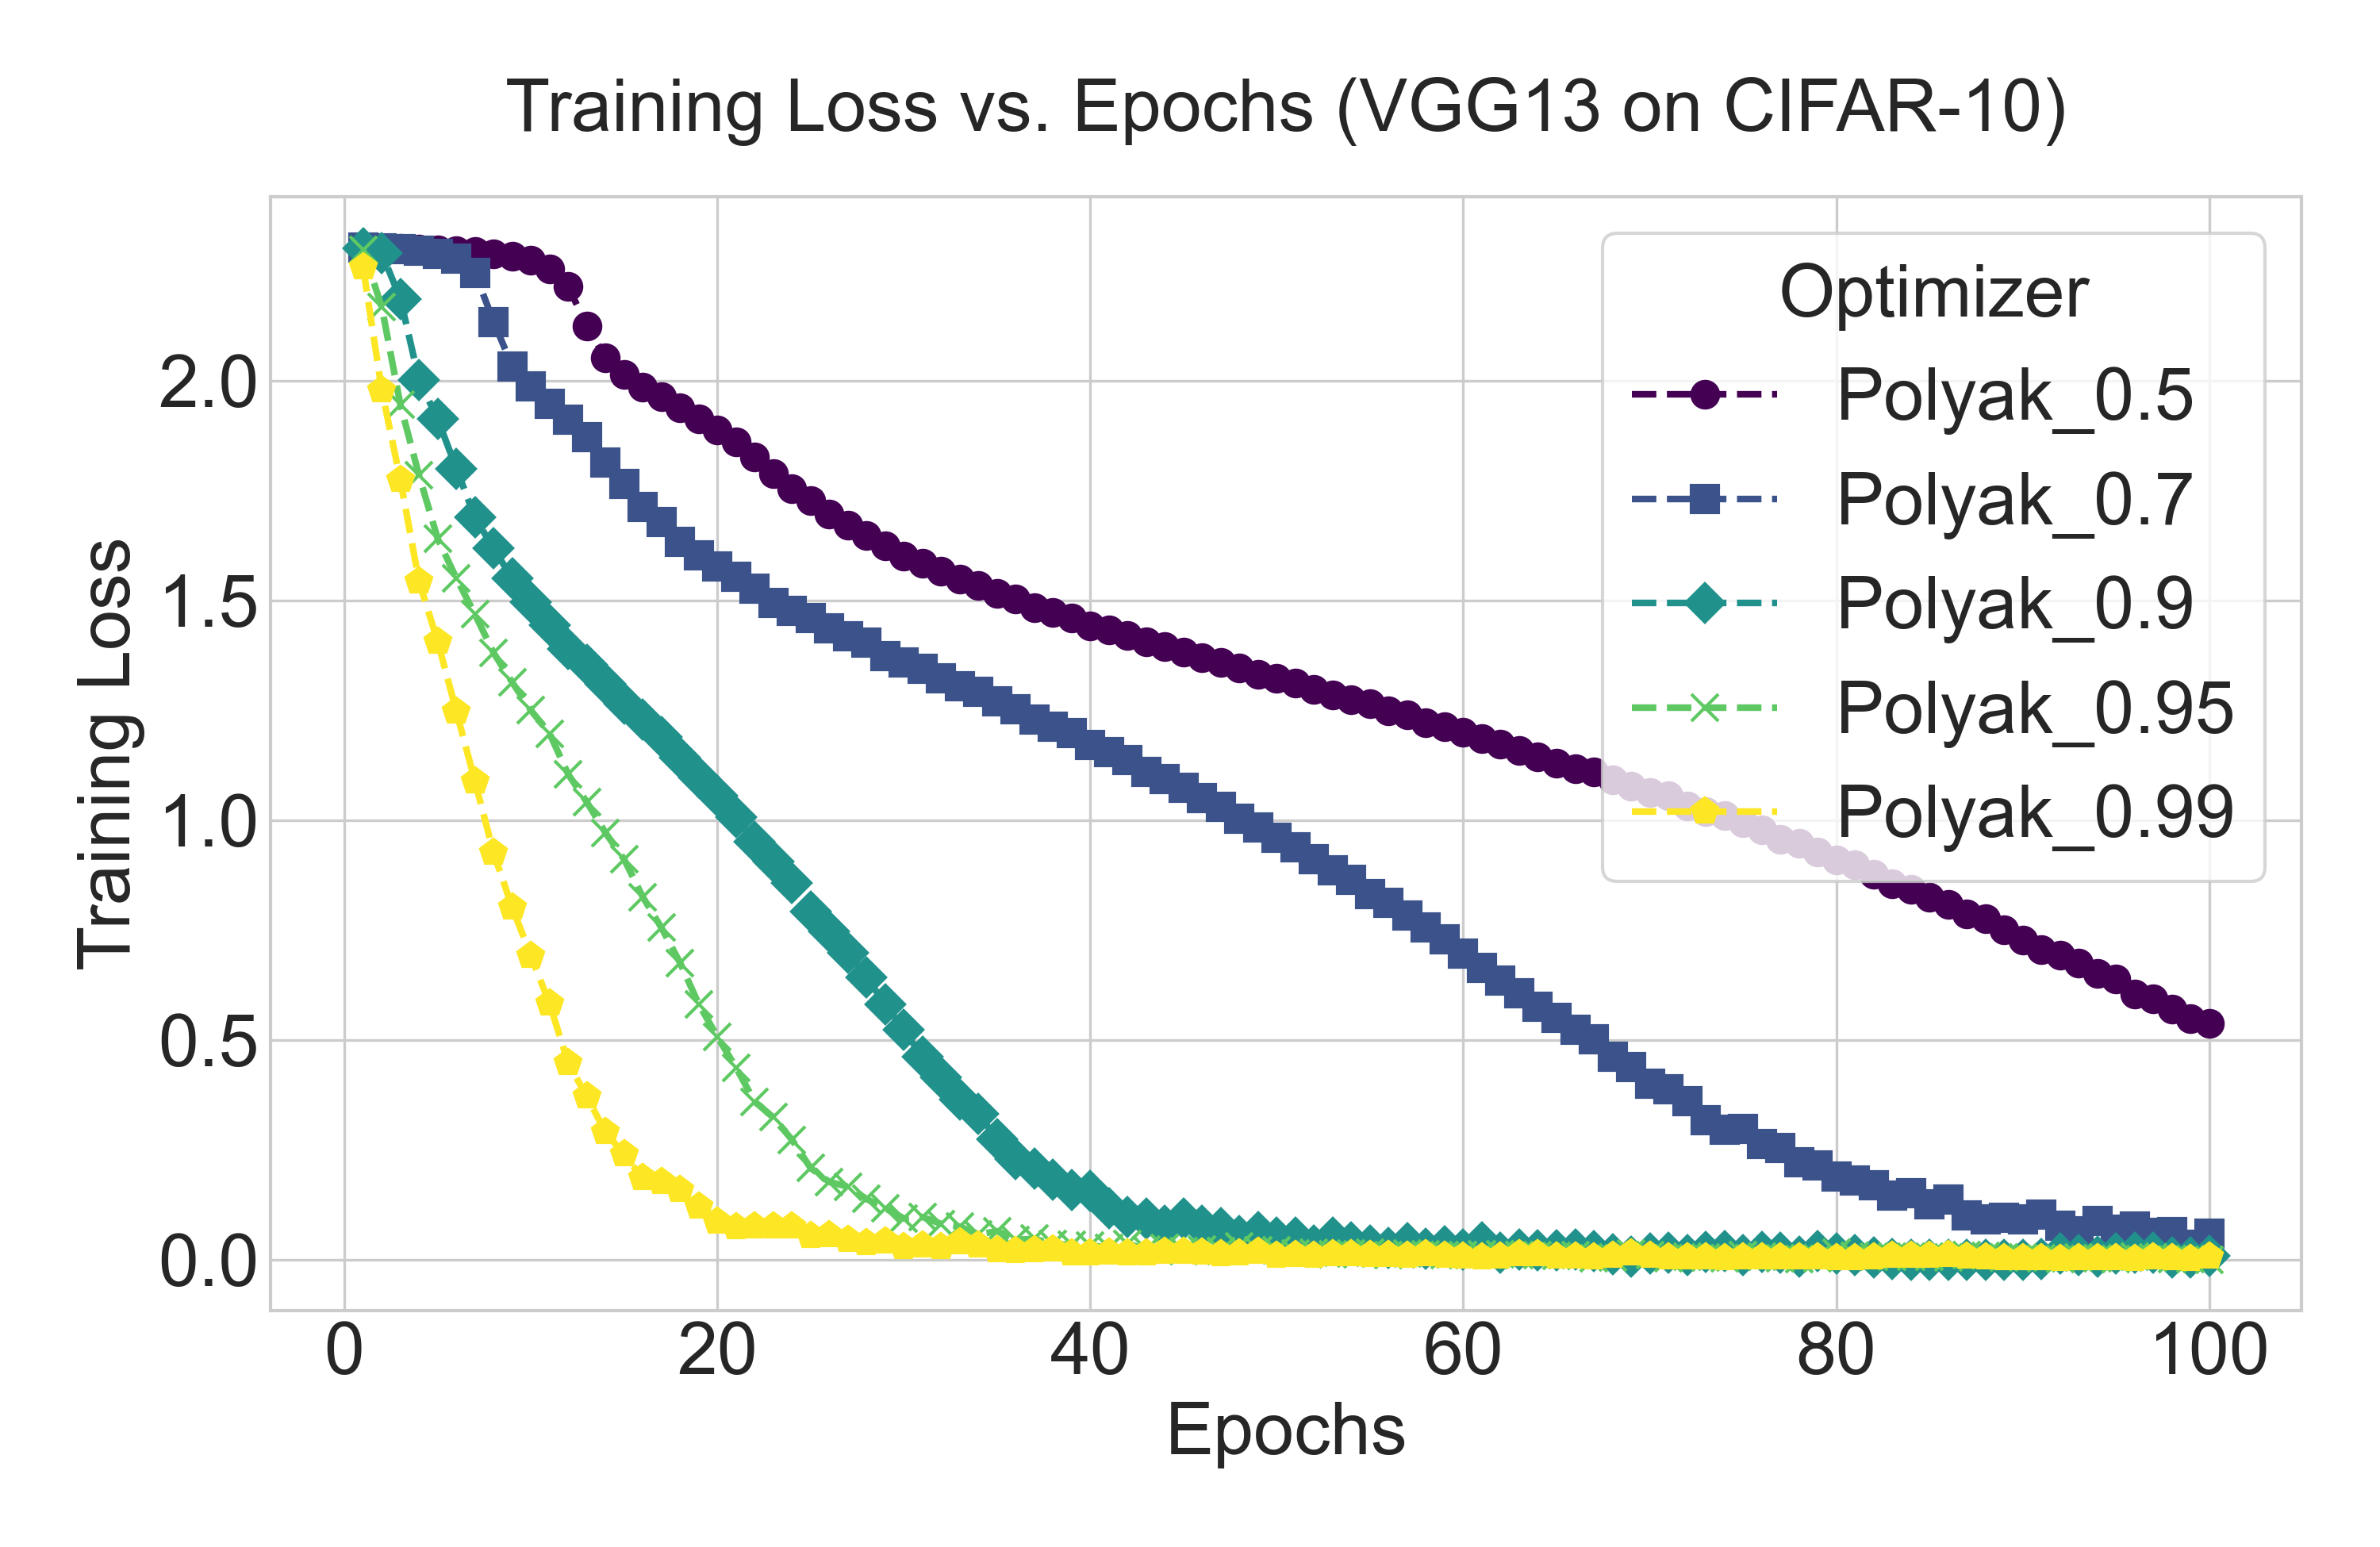
\includegraphics[width=0.48\textwidth]{Analysis_5_Polyak_Momentum3_cifar_vgg13_training_loss.png}} \quad
    \subfloat[VGG13 Accuracy on CIFAR-10]{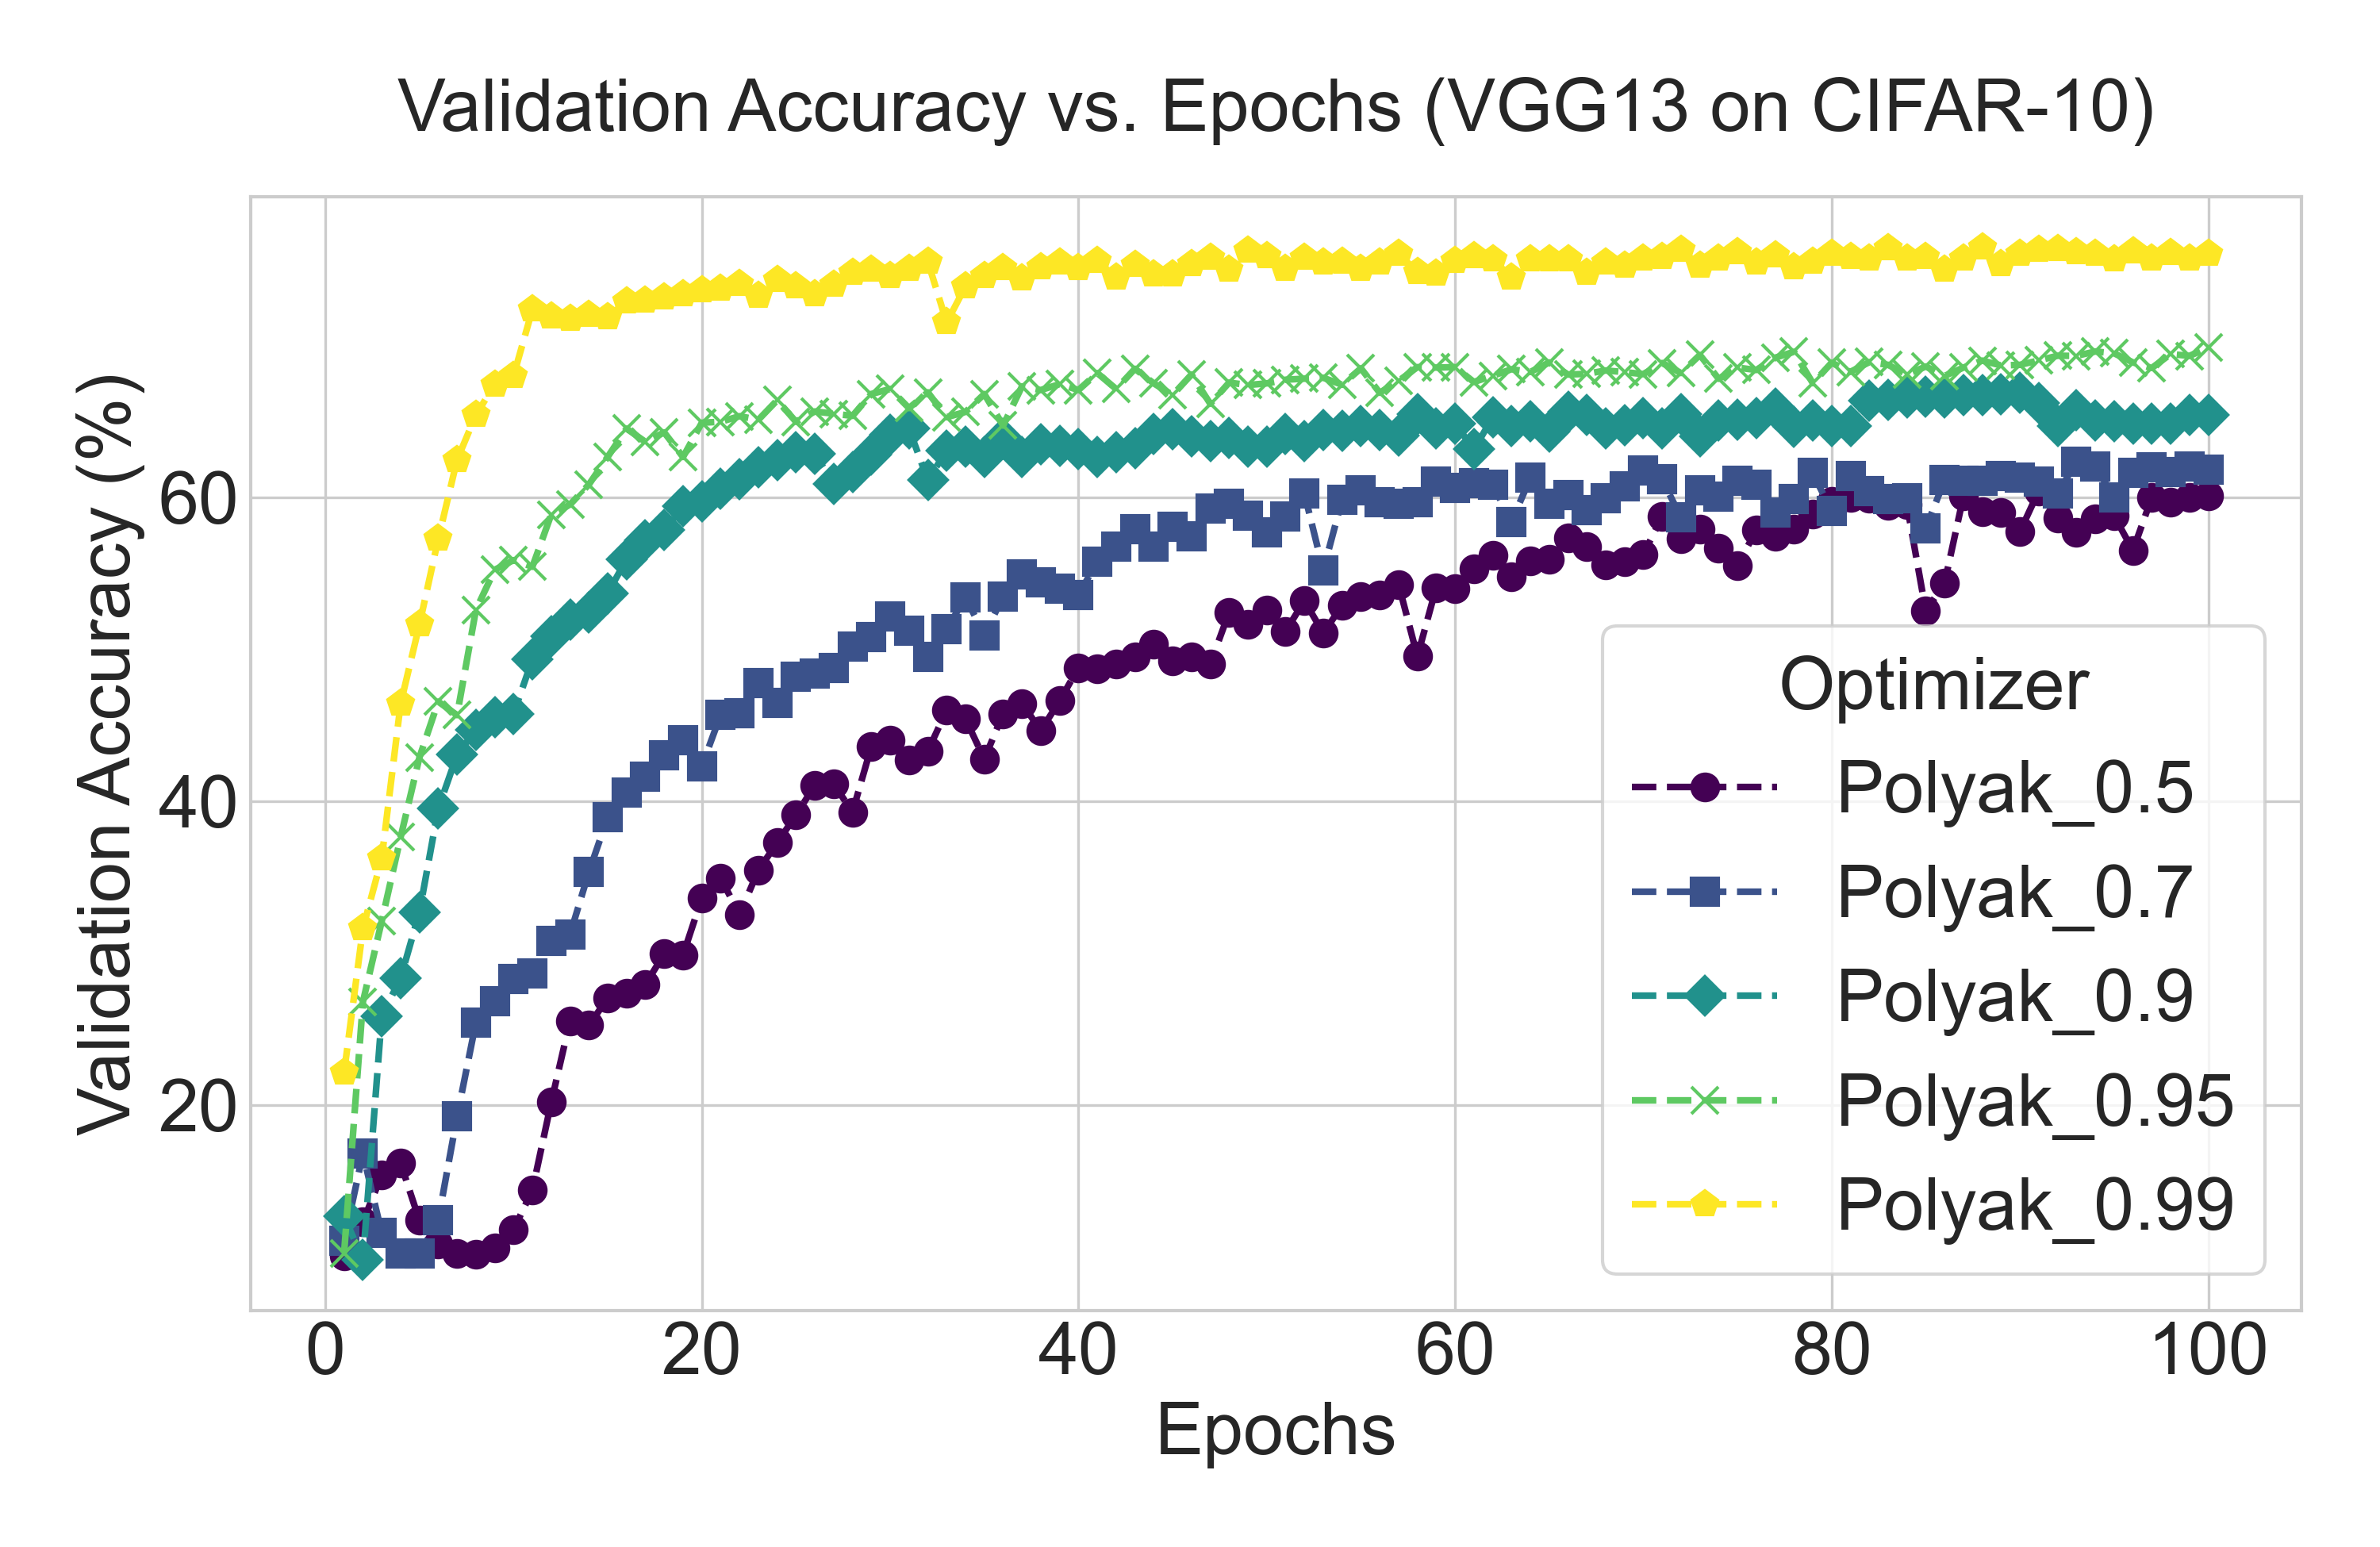
\includegraphics[width=0.48\textwidth]{Analysis_5_Polyak_Momentum3_cifar_vgg13_validation_accuracy.png}}
    \caption{Impact of Polyak momentum: baseline method (SGD, black line) vs. baseline method with Polyak momentum (purple line)}
    \label{fig:polyak_momentum_study}
\end{figure}


%%%%%%%%%%%%%%%%%%%%%%%%%%%%%%

\clearpage
\begin{thebibliography}{99}

\bibitem{adagrad}
Duchi, J., Hazan, E., & Singer, Y. (2011). 
Adaptive Subgradient Methods for Online Learning and Stochastic Optimization. 
\textit{Journal of Machine Learning Research}, 12, 2121–2159.

\bibitem{rmsprop}
Tieleman, T., & Hinton, G. (2012). 
Lecture 6.5—RMSProp: Divide the gradient by a running average of its recent magnitude. 
\textit{COURSERA: Neural Networks for Machine Learning}.

\bibitem{adam}
Kingma, D. P., & Ba, J. (2015). 
Adam: A Method for Stochastic Optimization. 
\textit{International Conference on Learning Representations (ICLR)}.

\bibitem{momentum}
Polyak, B. T. (1964). 
Some Methods of Speeding up the Convergence of Iteration Methods. 
\textit{USSR Computational Mathematics and Mathematical Physics}, 4(5), 1–17.

\bibitem{nesterov}
Nesterov, Y. (1983). 
A method for unconstrained convex minimization problem with the rate of convergence O(1/k\textsuperscript{2}). 
\textit{Soviet Mathematics Doklady}, 27(2), 372–376.

\end{thebibliography}



\end{document}